\documentclass[conference]{IEEEtran}
\usepackage[ruled,vlined]{algorithm2e}
\usepackage{amsmath}
\usepackage[english]{babel} %localisation
\usepackage{caption,subcaption} %supposedly incompatible with Springer and IOP, IEEETran and ACM SIG
\usepackage{cite} %nice citations, e.g. [1--5]
\usepackage{fixltx2e} %fix latex bugs
\usepackage{graphicx}
\PassOptionsToPackage{hyphens}{url}\usepackage{hyperref} %clickable URLS
\usepackage[htt]{hyphenat} %hyphenate \texttt
\usepackage{microtype} %makes text pretty; also condenses
\usepackage{multirow} %multiple rows in tables
\usepackage{siunitx,textcomp} %\SI{value}{unit}, \si{unit}; textcomp for microtype compatibility
%\usepackage [caption=false]{subfig} %if caption/subcaption not available
% \usepackage{tikz,pgfplots} %drawings and plots
\usepackage[siunitx]{circuitikz} %circuit figures
\usepackage[T1]{fontenc} %ensure proper hyphenation and treatment of math in sentences
\usepackage{booktabs}
\bibliographystyle{IEEEtran}

\usepackage{tikz}
\usepackage{verbatim}
\usepackage{listings}
\usepackage{pgfplots}
\begin{document}
\lstset{defaultdialect=[x86]{Assembler}}

% paper title
% can use linebreaks \\ within to get better formatting as desired
\title{Side Channel Analysis of an Embedded/Hardware Crypto Device}

% author names and affiliations
% use a multiple column layout for up to three different
% affiliations
\author{\IEEEauthorblockN{Sam Mitchell and Nathanael Weidler}
\IEEEauthorblockA{Deptartment of Electrical and Computer Engineering\\
Utah Stat University\\
Logan, Utah 84322\\
e-mail: samuel.alan.mitchell@gmail.com, NWeidler@gmail.com}
}

% make the title area
\maketitle


\begin{abstract}
%\boldmath
% Summarize project and results (executive summary).
%
This paper describes a side channel analysis attack on a microprocessor.  The microprocessor is running a Data Encryption Standard (DES) algorithm.  The goal of the attack is to recover the secret key from the device.  This is done by capturing the power usage of the device and using differential power analysis to analyze the data. 
 
\end{abstract}

\begin{IEEEkeywords}
Data Encryption Standard, Differential Power Analysis, Correlation Power Analysis, Security.
\end{IEEEkeywords}

\section{Introduction}
	Side channel analysis is one way to attack even the most computationally complex cryptographic devices.  Through side channel analysis, information (such as secret keys) can be obtained from devices without using more traditional or brute force attacks.  In order to carry out a side channel analysis attack, the attacker must have access to the device.  The attacker then obtains power information using an oscilloscope connected to a resistor put in series with the device's power input.

	In this paper a side channel analysis will be carried out on an Tiva-C  microprocessor to obtain the secret key from a Data Encryption Standard (DES) algorithm.  First, a typical DES implementation was written and loaded into the flash of the Tiva-C microprocessor.  Next, the side channel analysis was carried out.  After the power information, or traces, were obtained, a technique called differential power analysis (DPA) was used to analyze the data.  Another analysis using correlation power analysis was also carried out.  \cite{des} \cite{Messerges}


\subsection{Structure of paper}
	The organization is as follows: in Section \ref{sec::des_impl}, the development of the DES implementation is presented.  In Section \ref{sec::expr} the experimental test setup for the capturing of the traces is described. Section \ref{sec::analysis} contains the analysis of the data.  Conclusions are detailed in Section \ref{sec::conclusion}. 


\section{DES Implementation} \label{sec::des_impl}
	As a part of this work an implementation of DES was written for the Tiva-C microprocessor.  "The DES Algorith Illustrated" was a valuable resource during this process.  All of the explicit details of DES will be left to other work, however, a brief overview will be presented in order for the reader to grasp the complexity of the algorithm. \cite{des}

	DES is a 16 round encryption algorithm.  It works on 64-bit blocks of plaintext and outputs encrypted data of the same size.  The output of the algorithm is the cipher text.  The first step in DES is to divide the plaintext block in half, the left 32-bits and the right 32-bits.  The heart of DES is the 56-bit master key which is used to create 16 distinct 48-bit round keys, one for each round of the algorithm.  (The intent of this attack is to recover the key from the 16th round, from which all other keys can be easily obtained.)  To create each round key the 56-bit key is permuted and divided into two halves.  Then for each round each of those halves is shifted, recombined and permuted yielding the 48-bit round keys.

	One half of the plaintext (32-bits) is expanded and permuted to create a 48-bit word which is xored with the round key.  The result is divided into 8 6-bit parts which go through 8 distinct s-boxes.  An s-box is  method to substitute a 6-bit input with a 4-bit output.  These 4-bit outputs are put back together and permuted to create a 32-bit word which is xored with the other half of the plaintext.  This process is repeated 16 times until finally the two halves are put back together and permuted one last time to create the cipher text.  An illustration of one round is shown in figure \ref{fig:round}.

	\begin{figure}[h]
	\centering
	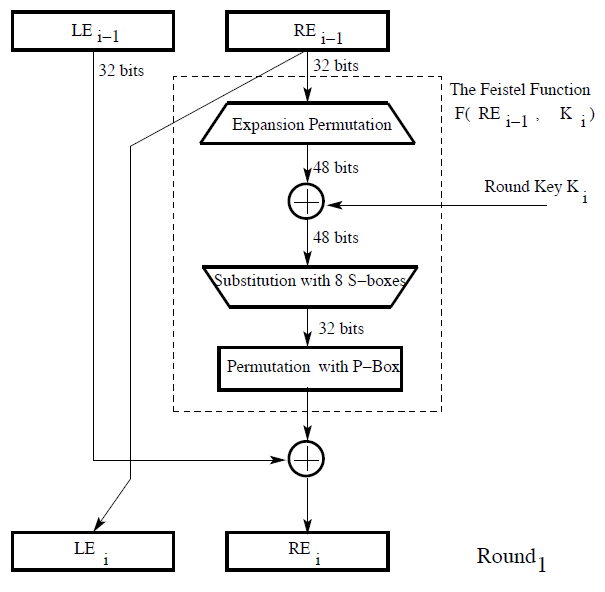
\includegraphics[width=0.7\linewidth]{./round}
	\caption{One round of DES.}
	\label{fig:round}
	\end{figure}

\subsection{DES Modifications}
	In order to facilitate the process by which traces are obtained, there was an addition to the traditional DES algorithm.  This slight modification in no way compromises the integrity of the algorithm or its outputs.  The change was to hold a general purpose input/output (GPIO) high during the algorithm except during a single instruction in which the output of the Feistel function is xored with the other half of the plaintext in round 16 and the result is written back to a register.  This allowed an oscilloscope to be triggered on the falling edge of the GPIO and frame this critical step which will be discussed later.  There were also two no-operations (nops) added before this register write and one after to allow the GPIO to settle and facilitate a cleaner capture.  The output of the assembly dump with comments added can be seen in figure \ref{fig:asm_snippet}.  Note that the register where the xor is written to (R0) is set to zero before the output of the xor is written there.
	
	\begin{figure}[h]
	\centering
	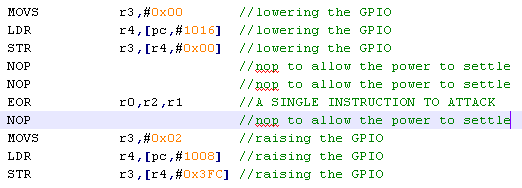
\includegraphics[width=0.7\linewidth]{./asm_snippet}
	\caption{The assembly showing the GPIO writes surrounding the xor and register write under attack.}
	\label{fig:asm_snippet}
	\end{figure}

	

\section{Experimental Setup} \label{sec::expr}
	This portion of the experiment was the most crucial to its success.  The goal is to obtain information about the power usage of the microprocessor during a critical step of the DES algorithm.  During a register write operation the power used will be different depending on the value of the word written.  It is believed that by analyzing this information, the secret key to the algorithm can be obtained.
	
	The oscilloscope used was a Techtronix DP0-2024 the sample rate was 1Gs per second and each trace contained about 270 samples.  The Tiva-C used a 17 MHz clock so there 38.5 samples per clock.
	
	The setup used involved the Tiva-C microprocessor powered by a bench top power supply through a breadboard.  The ground connection between the microprocessor and the power supply had a 1-$\Omega$ resistor added in series.  An Oscilloscope probe was placed on the resistor so that the voltage could be measured.  Then another oscilloscope probe was placed on the GPIO pin discussed in the previous section to act as the trigger.  The voltage data would be taken twenty times for each plain text value used in the DES algorithm and then averaged in an attempt to reduce noise.  91,840 captures with 4,592 unique plain text values would be obtained.  Each trace takes about two seconds to capture so the time to obtain all traces is 183,680 seconds or about 51 hours.  The voltage data acquired would be analyzed later to determine the secret key.  The test setup is illustrated in figure \ref{fig:bench}

	\begin{figure}[h]
	\centering
	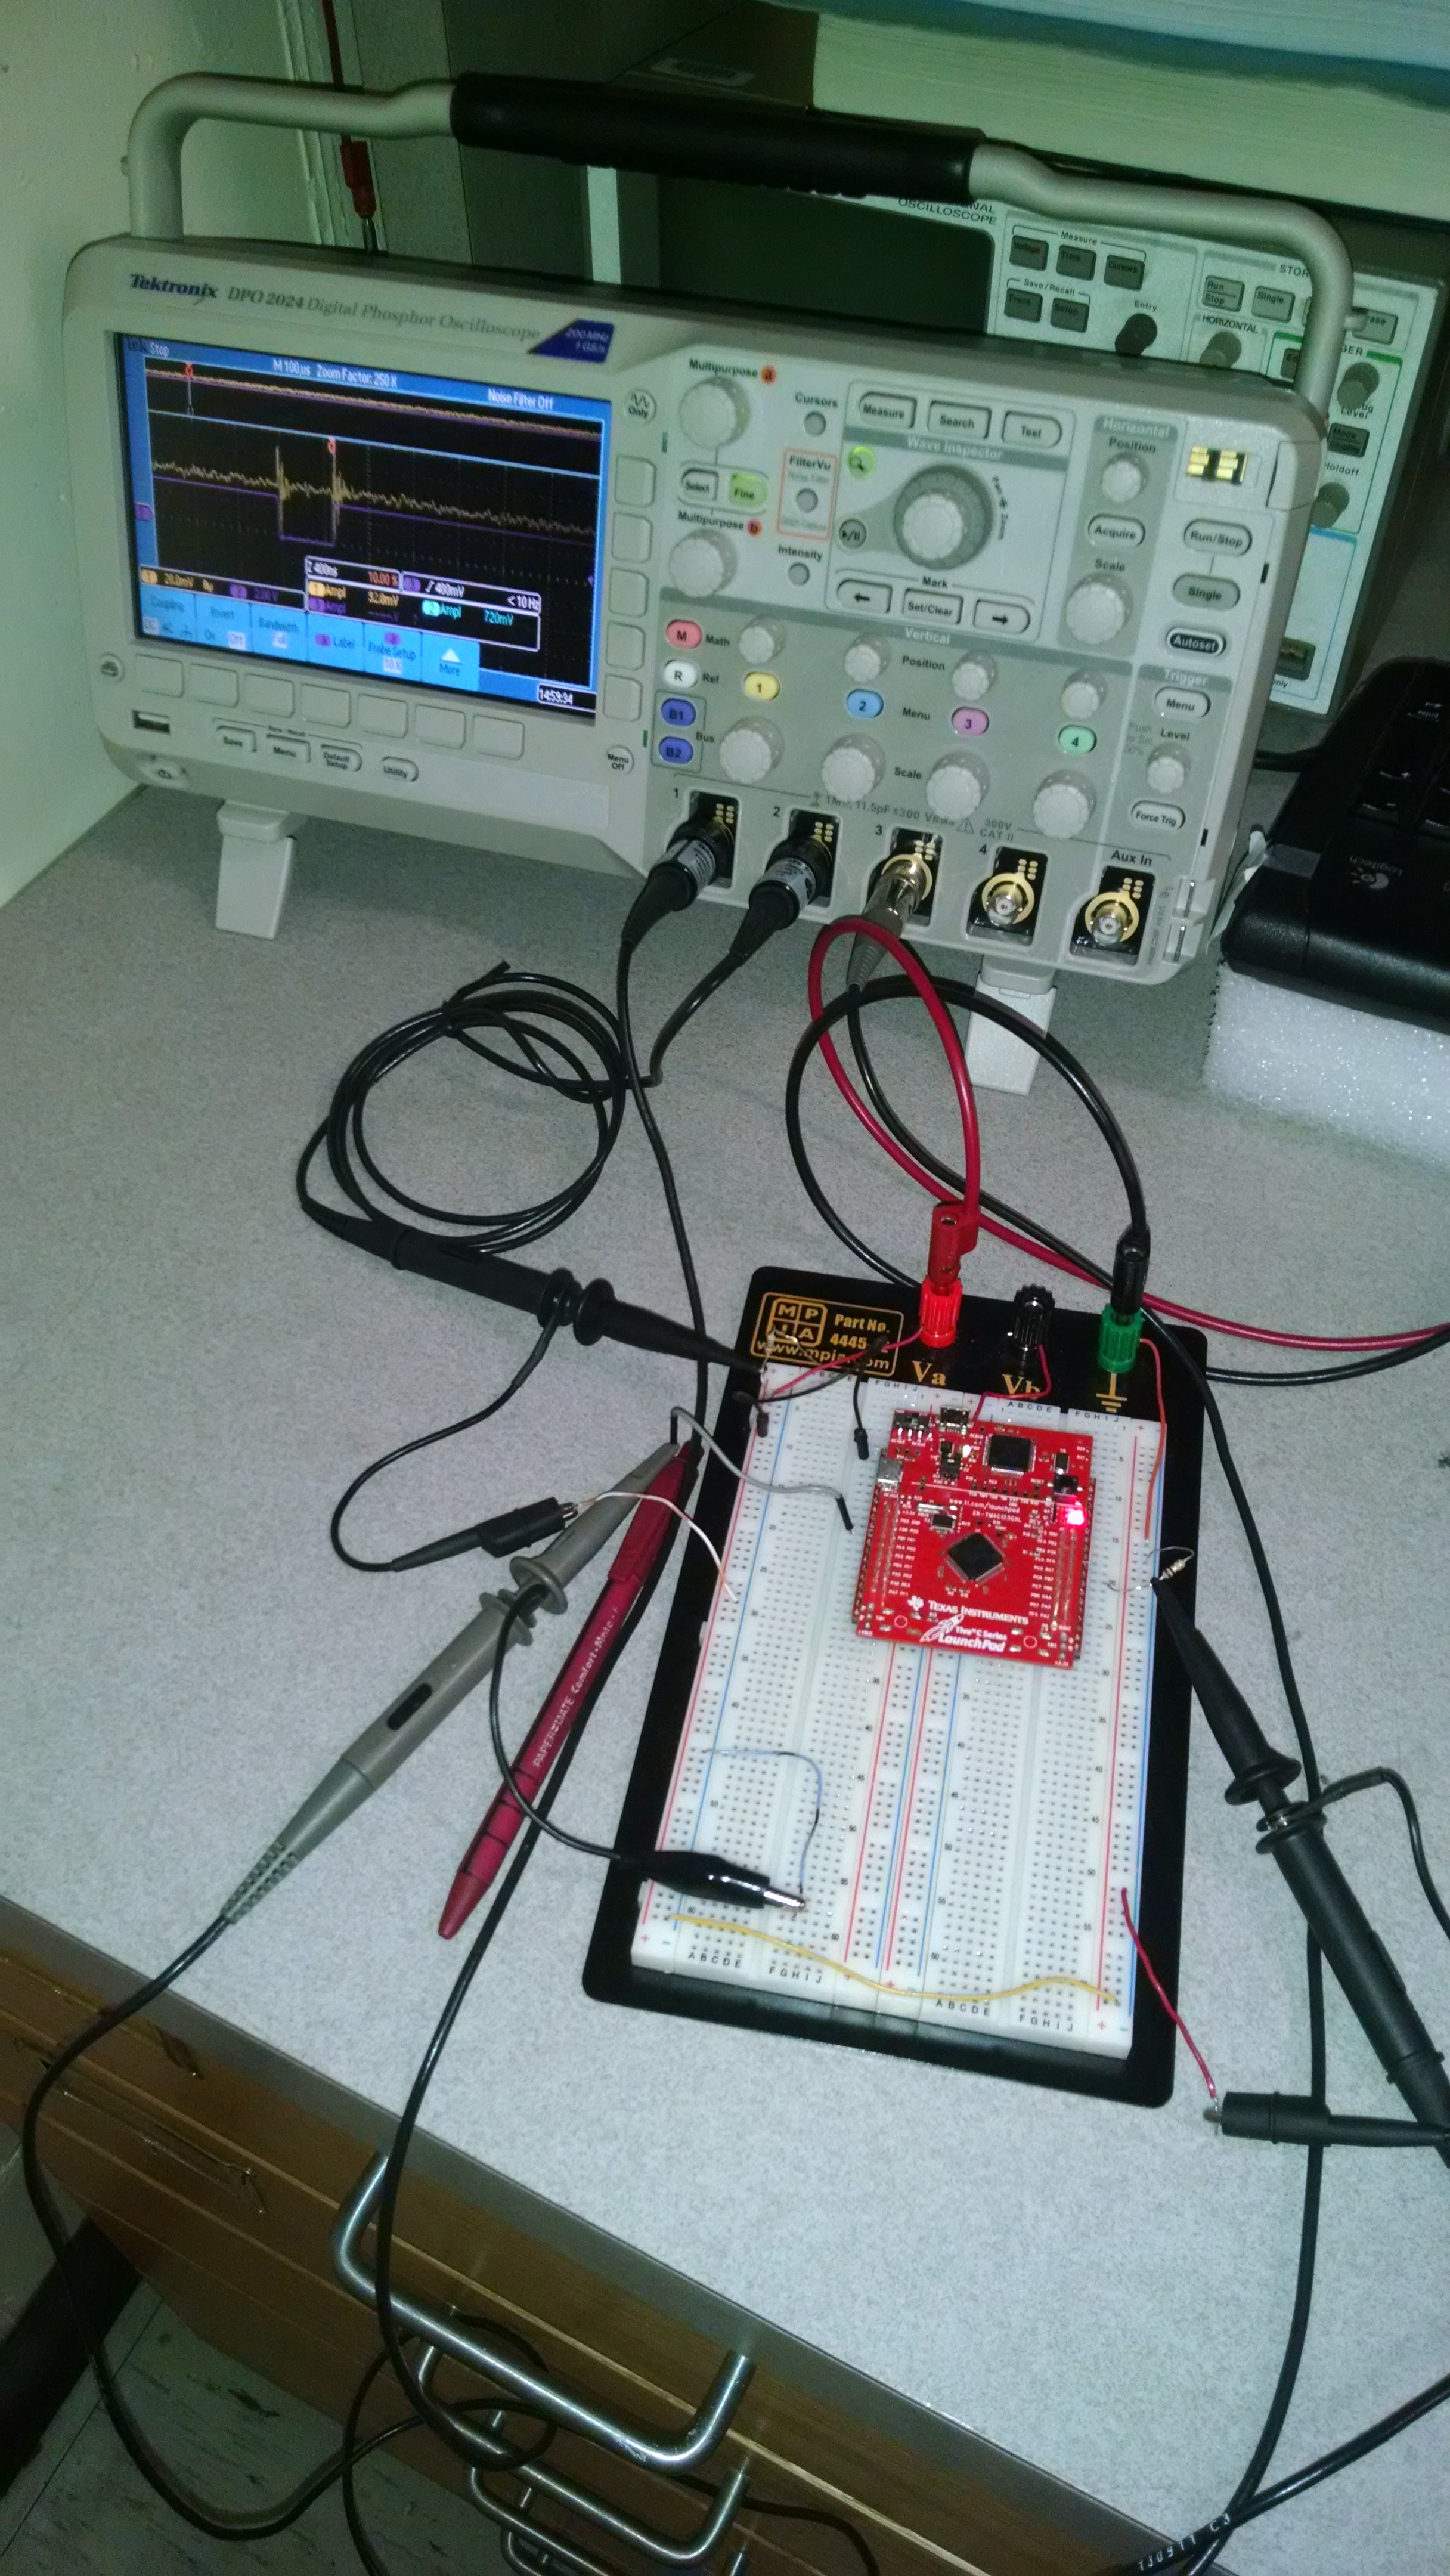
\includegraphics[width=0.7\linewidth]{./bench}
	\caption{Test setup showing the oscilloscope connected to the Tiva-C board.}
	\label{fig:bench}
	\end{figure}
	
	The test setup needed to be automated to facilitate the capturing of the traces.  In order for this to be done a matlab file was written to interface with the oscilloscope.  As trivial as this may sound it was not easy.  It took many hours of learning the oscilloscope and the commands to control it through matlab.  It also took time and patience to fine tune the DES implementation to create enough delay between each run of the algorithm to allow for the oscilloscope to transfer the data capture and re-arm itself.
	

\section{Analysis of the Data}\label{sec::analysis} 
\subsection{Differential Power Analysis}
	In order to analyze the data, differential power analysis (DPA) was employed.  Round 16 was chosen for this because given the cipher text, the input to the Feistel function and the output from the second xor (seen in the bottom right of figure \ref{fig:round}) can be determined.  Then the round key is guessed 6 bits at a time.  This greatly reduces the complexity of the key as there are only 64 possible combinations for a guess of 6 bits of the key.  Using knowledge of the Feistel function and the 6-bit key guess, the output of the Feistel function can be guessed at 4 bits at a time.  Remember, the s-boxes reduce the data from 48 bits to 32 bits.  This output is xored with the D value, and we already know the output of this xor.  So guessing one input and knowing the output determines the other input to the xor gate.  
	
	For each key guess 4-bits of the D word are deduced.  These 4-bit groups are divided into 3 sets where set 0 contains all guesses for which the four bits guessed are "0000," set 1 contains all guess where the 4 bits are "1111," and set 2 contains all other guessed values.  The average power for each sample point for sets 0 and 1 is calculated.  The two average powers are subtracted from each other.  The correct key guess will show large spikes where the calculation was actually made on the trace.  This is where the difference between the 2 sets of data is the greatest.  This process is repeated 8 times, once for each s-box until the correct key is determined.
	
\subsection{Correlation Power Analysis}
  Correlation Power Analysis (CPA) was also used on the data captured to see if more clear results could be obtained than what DPA provided.  In CPA the guessed at D word is sorted using the hamming distance of the change in the register value.  I our case the register was always set to 0 prior to the calculation, so in this case the Hamming distance is the same as the Hamming weight of the result.  Hamming weight is the number of 1s a data word contains.  The Hamming distance is the number bit changes from one word to the next so you count the number of 0s that changed to 1s and add that number to the number of 1s that changed to 0s.  The Hamming distance of anything from 0 is the Hamming weight of the data word.
  Each sample from every trace is entered into Pearson's sample correlation coefficient along with the Hamming weight of the guess.  The result should show a high correlation for the correct key guess.  The key guesses are the same 6-bit key guesses that were used in the DPA attack.

\subsection{Actual Key Values Analysed}
  This experiment is unique from an actual side channel analysis attack because we knew what the secret key was.  This meant that we could run the correct values through DPA and CPA as was done previously with guesses.  The results will be discussed in the next section.

\section{Conclusion}\label{sec::conclusion} 


% Summarize results and lessons learned.
	Both DPA and CPA have previously been shown to work at recovering secret keys from DES.  We were not able to reproduce such promising results.  We still believe that DPA and CPA should work to recover secret keys from DES but there were some potential flaws in our methods.
  One aspect to this project which could have been done better would have been to take more traces for a single plain text value.  We took 20 traces for each plain text, but we believe that if we had taken many more than this the noise would have averaged out more nicely and the results may have been better.  Perhaps we should have taken an order of magnitude more traces than what we did.  We believe that this was the main contributing factor to the side channel attacks not producing the expected results.
\bibliography{report}
% that's all folks

  \begin{figure}[h]
  % This file was created by matlab2tikz.
% Minimal pgfplots version: 1.3
%
%The latest updates can be retrieved from
%  http://www.mathworks.com/matlabcentral/fileexchange/22022-matlab2tikz
%where you can also make suggestions and rate matlab2tikz.
%
\definecolor{mycolor1}{rgb}{0.00000,0.75000,0.75000}%
\definecolor{mycolor2}{rgb}{0.75000,0.00000,0.75000}%
\definecolor{mycolor3}{rgb}{0.75000,0.75000,0.00000}%
%
\begin{tikzpicture}

\begin{axis}[%
width=4.822222in,
height=3.803333in,
at={(0.808889in,0.513333in)},
scale only axis,
separate axis lines,
every outer x axis line/.append style={black},
every x tick label/.append style={font=\color{black}},
xmin=0,
xmax=300,
xlabel={Time (Sample)},
every outer y axis line/.append style={black},
every y tick label/.append style={font=\color{black}},
ymin=-0.06,
ymax=0.06,
ylabel={Correlation coefficient},
title={CPA Attack. sbox 1 Key 60}
]
\addplot [color=blue,solid,forget plot]
  table[row sep=crcr]{%
1	0.0071642927051821\\
2	0.00823800161419562\\
3	0.00851185026142069\\
4	0.00975339194226313\\
5	0.00898433441926672\\
6	0.00631928732454859\\
7	0.00234014000585978\\
8	0.00175928597549637\\
9	0.00235730282690148\\
10	0.00335333131003443\\
11	0.00250465043415322\\
12	-0.00316103965423727\\
13	-0.00796909846051079\\
14	-0.00624749052998818\\
15	-0.00290335049989134\\
16	-0.00303647642881052\\
17	-0.00495777397026073\\
18	-0.0111419761129397\\
19	-0.00707808301783961\\
20	-0.00586715628580042\\
21	-0.00810035816953473\\
22	-0.00206931323277037\\
23	0.00223100309549707\\
24	0.00182476548238758\\
25	-0.000619402544366933\\
26	-0.00303788905965822\\
27	-0.00495866073973687\\
28	-0.00668468927861703\\
29	-0.0038424989773569\\
30	0.000655714727758218\\
31	0.00372856883696158\\
32	0.00323424291372684\\
33	0.00286931033810634\\
34	-0.000624434124169192\\
35	-0.00136347422159206\\
36	0.000747676205935821\\
37	0.00312261992364439\\
38	0.00219683309625941\\
39	0.00142436142970316\\
40	-0.000801879621378517\\
41	-0.00404223109399184\\
42	-0.00538481975082091\\
43	-0.00584244089425078\\
44	-0.00608906463398731\\
45	-0.00645376898832837\\
46	-0.00781310094413041\\
47	-0.011397698635143\\
48	-0.0163429921547954\\
49	-0.0190807597668261\\
50	-0.0205603018699155\\
51	-0.0199311162174008\\
52	-0.0116982109939233\\
53	-0.0048526378586434\\
54	-0.00123176421519794\\
55	-3.7468456776188e-05\\
56	-0.00269229041572839\\
57	-0.00545554612938253\\
58	-0.00388855010613452\\
59	0.000468755048120498\\
60	0.00436405527202178\\
61	0.00791583582388235\\
62	0.00719266478010392\\
63	0.00797892003092513\\
64	0.00868647774757552\\
65	0.00487902238868642\\
66	0.00776791241816503\\
67	0.00892895094009628\\
68	0.0094865359162294\\
69	0.00882803913424448\\
70	0.00833974892787191\\
71	0.00575667019358304\\
72	0.00272459956253976\\
73	-0.000215977666105271\\
74	-0.00131421499249859\\
75	-0.00262719013813163\\
76	-0.00206841590638223\\
77	-0.00424379310668877\\
78	-0.00559725945579634\\
79	-0.0050635210331703\\
80	-0.00424110944976987\\
81	0.000479935651774295\\
82	0.00378503590927323\\
83	0.00751457514388466\\
84	0.00622300306929064\\
85	0.00485160830667056\\
86	-2.63103482933913e-05\\
87	-0.0015499417460501\\
88	-0.00116886446379578\\
89	-0.0033373192320123\\
90	-0.00336768130026785\\
91	-0.00368843571432128\\
92	-0.0036599656770139\\
93	-0.00437888116092525\\
94	-0.00511826968209743\\
95	-0.00340030779566844\\
96	0.000192161513480936\\
97	-0.000812382997288947\\
98	-0.00186403260506426\\
99	-1.39234279046771e-06\\
100	-0.00151545540656137\\
101	-0.00117560845215566\\
102	0.000211030532255539\\
103	0.000209191010659364\\
104	0.000593646532450531\\
105	0.00605638013232833\\
106	0.00662347444003311\\
107	0.00811469646764876\\
108	0.00659132000189058\\
109	0.00443733489161988\\
110	0.00190970860452063\\
111	0.000936451694926619\\
112	-0.000409155909899822\\
113	-0.000479279303921271\\
114	0.000251182606060506\\
115	-0.00227385077439074\\
116	-0.00230561845645721\\
117	-0.00221689200485501\\
118	-0.00610589583129329\\
119	-0.0108457866601835\\
120	-0.0150428864105645\\
121	-0.01606515488144\\
122	-0.0159119742159936\\
123	-0.0140603753328423\\
124	-0.0181467243559562\\
125	-0.0173348609211415\\
126	-0.0160995474333485\\
127	-0.0125822677237165\\
128	-0.0110606929126225\\
129	-0.0113828584685067\\
130	-0.00992579381645373\\
131	-0.00944035327867381\\
132	-0.00936832427059649\\
133	-0.00630359378570392\\
134	-0.00253539030535765\\
135	-0.000677714069490746\\
136	0.000993004642435525\\
137	0.00479309124589737\\
138	0.00472006055968577\\
139	0.00511401971671127\\
140	0.00620898397983047\\
141	0.00288769333532856\\
142	0.00113280305148649\\
143	-0.00300287535258287\\
144	-0.00242221900926271\\
145	-0.00487476756441233\\
146	-0.00213592411181027\\
147	-0.00592856329560425\\
148	-0.00638000639493625\\
149	-0.00518647597832688\\
150	-0.00329844411262867\\
151	-0.00469969005796588\\
152	-0.00848068924470645\\
153	-0.00914664206563172\\
154	-0.0121306536244821\\
155	-0.0136342949972969\\
156	-0.0137470385499118\\
157	-0.0111744471589243\\
158	-0.00981837810238808\\
159	-0.0112120920233249\\
160	-0.0124737465230043\\
161	-0.00945167268925162\\
162	-0.00728237631390811\\
163	-0.00881890906886865\\
164	-0.00525427679097711\\
165	-0.00300712735553761\\
166	-0.0033268196358555\\
167	-0.00610330837737837\\
168	-0.00750506666806108\\
169	-0.00880603644329622\\
170	-0.00855232996015349\\
171	-0.00967708406223929\\
172	-0.0117544588623611\\
173	-0.0104682575445289\\
174	-0.00625619339777921\\
175	0.00145523154732568\\
176	0.00777941912301079\\
177	0.0085178237732707\\
178	0.00328372948907595\\
179	-0.000352059930464952\\
180	-0.001524448288565\\
181	-0.00392204365060214\\
182	-0.00352730086077768\\
183	-0.00124739891334282\\
184	0.00335540016864439\\
185	0.00151027636420142\\
186	-0.000814081629743965\\
187	0.00144210491605376\\
188	0.00597625801698691\\
189	0.00412576315621165\\
190	0.00392628055812437\\
191	0.00645385324913347\\
192	0.00627527429506374\\
193	0.00430203931780065\\
194	0.00302277424546133\\
195	0.00590295700686696\\
196	0.00894767573501765\\
197	0.00750084921177538\\
198	0.00549293903714462\\
199	0.00807420147777425\\
200	0.0075861357006196\\
201	0.00583327851307139\\
202	0.00585622950507873\\
203	0.0023627859003102\\
204	0.00170876866076364\\
205	0.00263925290228968\\
206	0.00041621843212702\\
207	0.00030540170734188\\
208	-0.0046262458506214\\
209	-0.0073247388858498\\
210	-0.00839184853451314\\
211	-0.00815613626187292\\
212	-0.00852101138716287\\
213	-0.00694376475725508\\
214	-0.00198695169369213\\
215	0.0012131557715529\\
216	0.00381748429992131\\
217	0.00640437523430049\\
218	0.00614867012701899\\
219	0.00767436028754151\\
220	0.01296224660687\\
221	0.0138018244710181\\
222	0.0172871862100402\\
223	0.0148821191203837\\
224	0.0127662492501776\\
225	0.00997314523855585\\
226	0.0104863915616543\\
227	0.0109512353084008\\
228	0.0116934789575744\\
229	0.013137358468437\\
230	0.0109294929775824\\
231	0.00948947555653021\\
232	0.0112750587114855\\
233	0.0133985520844322\\
234	0.0146374922601958\\
235	0.0136124431198085\\
236	0.00920858358705993\\
237	0.00715291483471399\\
238	0.00435175162914697\\
239	0.00228077813666127\\
240	0.00357523965409502\\
241	0.000590580451468124\\
242	-0.000774738310712454\\
243	0.00164726749392138\\
244	-0.00090307959884816\\
245	-0.00255988717679691\\
246	-0.000827384872865029\\
247	0.00391489987501687\\
248	0.00790252458336657\\
249	0.00517582794403494\\
250	0.00348974488841968\\
251	0.00303842924454522\\
252	0.00547471060596576\\
253	0.00452914946265383\\
254	0.00751955946487708\\
255	0.00760011326071871\\
256	0.00480869000444095\\
257	-0.00589911693841208\\
258	-0.00853461290692797\\
259	-0.00256671172895152\\
260	0.00717911798771801\\
261	0.00818388749000545\\
262	-0.00278929782169989\\
263	-0.005837851599881\\
264	-0.00478519114321792\\
265	0.00630202641190493\\
266	0.00778871464345635\\
267	0.00826553537516558\\
268	0.00745717881996993\\
269	-0.00335125441031602\\
270	-0.00517477580888924\\
};
\addplot [color=black!50!green,solid,forget plot]
  table[row sep=crcr]{%
1	-0.0043671043398804\\
2	-0.00222247970029718\\
3	0.00273500419520813\\
4	0.00432994428367264\\
5	0.00931366755153294\\
6	0.0067572906191539\\
7	0.0034653653525761\\
8	0.0101159952477438\\
9	0.0103062603583583\\
10	0.00781601538988507\\
11	0.00747843861904305\\
12	-2.04995144265191e-05\\
13	0.00223207116611657\\
14	0.00896016916530077\\
15	0.00650477735319655\\
16	0.0090485514597503\\
17	0.0113171170486634\\
18	0.00918801757455248\\
19	0.00219452348456227\\
20	0.00396556494107594\\
21	0.0137809298071028\\
22	0.0119894341035289\\
23	0.00343085118605572\\
24	-0.00395061569148631\\
25	-0.00859322699607739\\
26	-0.00515570714040971\\
27	-0.00145653976793586\\
28	0.00422007993403049\\
29	0.00981757450509911\\
30	0.00377948814948566\\
31	0.00335724628397617\\
32	0.00648525204852015\\
33	0.0108117066813167\\
34	0.0113958026719403\\
35	0.0105929845142085\\
36	0.0122261673761213\\
37	0.00974179171691838\\
38	0.00698657029195456\\
39	0.00511376779900008\\
40	0.00331640556924368\\
41	0.00402587123023976\\
42	0.00260919408054725\\
43	0.000924326690349322\\
44	-0.00337649872816698\\
45	-0.00725493281131088\\
46	-0.00155300440271344\\
47	0.00173439929204084\\
48	0.00892860339306589\\
49	0.0154236126384246\\
50	0.0149215165543663\\
51	0.0185698586555175\\
52	0.0161434288888338\\
53	0.00857558310662472\\
54	0.0044342212658199\\
55	0.00400544894555228\\
56	0.00579314736677747\\
57	0.00583754371144608\\
58	0.00244299949541585\\
59	-0.000977275083534528\\
60	-0.00420347660752387\\
61	-0.00131114404690785\\
62	-0.00347165163942136\\
63	-0.00125645462750701\\
64	0.00189382664685785\\
65	0.00829842710134904\\
66	0.0121195794738187\\
67	0.0120380778278145\\
68	0.0117602005524432\\
69	0.00847776977563133\\
70	0.00640035894357252\\
71	0.00767463821425433\\
72	0.0102864366809456\\
73	0.0118582233731299\\
74	0.0127036881124544\\
75	0.0135323802779826\\
76	0.0111185241894341\\
77	0.00914190430803086\\
78	0.00558941747509383\\
79	0.0062980735972168\\
80	0.00352514979127443\\
81	0.000112412629313517\\
82	-0.0049890342240702\\
83	-0.00442330884560572\\
84	-0.00664052195544301\\
85	-0.00521016179911557\\
86	-0.000686497961817786\\
87	0.00459356985247461\\
88	0.00782434759718988\\
89	0.0100723292593469\\
90	0.00932312001362166\\
91	0.00518863985293186\\
92	0.00239781206731291\\
93	0.00181626026623047\\
94	0.00221895668679797\\
95	0.00178214092583709\\
96	-0.000353440821431199\\
97	-0.00162496682036596\\
98	0.00156810559590201\\
99	-0.000506715612036494\\
100	-0.000751161128209318\\
101	-0.00218445838464818\\
102	-0.00276827773221086\\
103	-0.00142823348389451\\
104	-0.000500181338907733\\
105	0.00127205313432777\\
106	0.00392171644330684\\
107	0.00371373417275958\\
108	0.00618340761368233\\
109	0.0080834047776519\\
110	0.00840480902323006\\
111	0.00789355246937493\\
112	0.0084849880707184\\
113	0.0117492318113948\\
114	0.00993563838929912\\
115	0.0153125946511684\\
116	0.0119030920453945\\
117	0.0106845189588748\\
118	0.0110540177795778\\
119	0.0104802985232886\\
120	0.00810496006870568\\
121	0.0106333364626365\\
122	0.0137220059925138\\
123	0.0148108159340836\\
124	0.0183722646463493\\
125	0.0184587179703967\\
126	0.0177228610680925\\
127	0.0161795961793933\\
128	0.0155386252803851\\
129	0.0133692871921022\\
130	0.00920367523548599\\
131	0.00227687917291977\\
132	-0.000673916684008519\\
133	-0.00277771263361567\\
134	-0.00224359306312196\\
135	-0.00145703686738362\\
136	-0.00457307901378279\\
137	-0.00683284464697657\\
138	-0.00975452825593099\\
139	-0.00892908254519684\\
140	-0.00590956034648586\\
141	-0.00467454636981026\\
142	-0.0027913174318508\\
143	-0.000736934663612563\\
144	-0.000521671029022046\\
145	0.0010714879484409\\
146	-0.000866734975798643\\
147	0.00114554211761755\\
148	-0.00472273749533247\\
149	-0.00389383998316968\\
150	-0.00064082164154131\\
151	0.00362544412999853\\
152	0.00904938033482482\\
153	0.0119917224545815\\
154	0.0131535176617645\\
155	0.0161130973716154\\
156	0.0158409349548333\\
157	0.0147531920607117\\
158	0.0140609511626791\\
159	0.0110585474533469\\
160	0.0118432640463403\\
161	0.00906530579004923\\
162	0.00388469323406883\\
163	0.00950398427832985\\
164	0.011210085536625\\
165	0.0119025961170318\\
166	0.013099666135207\\
167	0.0130375752171453\\
168	0.0131557853492465\\
169	0.013013008006423\\
170	0.0123732645998548\\
171	0.013654044883022\\
172	0.013917340627169\\
173	0.0138934973169565\\
174	0.0102411950098052\\
175	0.00606565501023991\\
176	0.00355649595214979\\
177	0.00416157712121371\\
178	0.00208506022169149\\
179	-0.00134635862188669\\
180	1.58551468977914e-05\\
181	-0.00233976804147667\\
182	-0.00467609930946381\\
183	-0.00585374054908655\\
184	-0.00675844329258017\\
185	-0.00470595762624047\\
186	-0.00464573826247764\\
187	-0.00563337928392984\\
188	-0.00666672618125195\\
189	-0.00722928219488545\\
190	-0.00824616587951608\\
191	-0.010174633745829\\
192	-0.0105314129556808\\
193	-0.00779544312187827\\
194	-0.00326064058484659\\
195	0.00117178766859721\\
196	0.00465631837685196\\
197	0.00531492246715188\\
198	0.00700538227248968\\
199	0.0049006596637597\\
200	0.00365488421378485\\
201	0.00553348538579397\\
202	0.010298073262056\\
203	0.0131819438399981\\
204	0.0152694883230485\\
205	0.0170559634705028\\
206	0.016234802472671\\
207	0.0180269114989398\\
208	0.0169216854741307\\
209	0.0181897441028367\\
210	0.0185791249071684\\
211	0.0187710495569786\\
212	0.0186093486904524\\
213	0.0176566977907194\\
214	0.0164060149556585\\
215	0.0125109045547498\\
216	0.00978326458822481\\
217	0.00748767152862969\\
218	0.00501228048709931\\
219	0.0024950342076763\\
220	0.000324857451814218\\
221	0.00200357291040873\\
222	0.00227874477254872\\
223	0.00434104151272892\\
224	0.0105200238142436\\
225	0.0140816656081873\\
226	0.0153890117644659\\
227	0.0167635454167548\\
228	0.015006710736721\\
229	0.0129083366176522\\
230	0.0116877286173054\\
231	0.0113508207648363\\
232	0.00884892415147847\\
233	0.0101477667337767\\
234	0.0123458648219561\\
235	0.013139051882848\\
236	0.0174474428427005\\
237	0.0170460278952076\\
238	0.0155441176599017\\
239	0.0133362860503227\\
240	0.013822691081112\\
241	0.0084308424717037\\
242	0.0024756401617634\\
243	0.00416032344075249\\
244	0.00659262728064975\\
245	0.00898468516151306\\
246	0.00969735946024103\\
247	0.013062239892794\\
248	0.00812826345523426\\
249	0.00696945274575818\\
250	0.00837433195539488\\
251	0.00426757826417186\\
252	0.00512158762511234\\
253	0.00530006566429868\\
254	0.0042169429433576\\
255	0.00845426181765253\\
256	0.00680262064432653\\
257	0.0109285466919135\\
258	0.00840434414146966\\
259	0.00222407955666588\\
260	-0.00501379433350216\\
261	-0.00194123371506259\\
262	0.0100629081271856\\
263	0.00860934327209188\\
264	0.00630566199351253\\
265	-0.00792264113615451\\
266	-0.0070614869261079\\
267	-0.00604940154600608\\
268	0.00169696731265892\\
269	0.00994355723282172\\
270	0.00707796649389725\\
};
\addplot [color=red,solid,forget plot]
  table[row sep=crcr]{%
1	-0.0247609539928959\\
2	-0.0215542353804128\\
3	-0.0205913996051899\\
4	-0.0207345496737225\\
5	-0.0205863142910779\\
6	-0.0205250055159155\\
7	-0.0220251364312423\\
8	-0.0308840956774567\\
9	0.000113300757944517\\
10	0.00436272808618463\\
11	-0.0150527724375817\\
12	-0.0217421571591836\\
13	-0.0284390552111535\\
14	-0.00391416814319086\\
15	0.00636072410716683\\
16	0.00674992841688767\\
17	-0.00146441261727157\\
18	-0.020932462211718\\
19	-0.0177956808352929\\
20	-0.0196458713201586\\
21	-0.0249786403477992\\
22	-0.0235766269538224\\
23	-0.0171078078445414\\
24	-0.02422173576826\\
25	-0.0323073173029716\\
26	-0.0272087448457657\\
27	-0.0196404941258212\\
28	-0.0143760039305551\\
29	-0.0107867576233688\\
30	-0.00699482839838469\\
31	-0.00953610072627832\\
32	-0.0143255139497505\\
33	-0.0180545521973678\\
34	-0.0174204218591591\\
35	-0.0172756582313983\\
36	-0.0215374464752468\\
37	-0.0246111623561417\\
38	-0.024017086853576\\
39	-0.0266442166194433\\
40	-0.0329185532866946\\
41	-0.0340534018937977\\
42	-0.0246770330549708\\
43	-0.0217036185866499\\
44	-0.0237503129837188\\
45	-0.0186953624711573\\
46	-0.0126334533972747\\
47	-0.00946655885969155\\
48	-0.00880341306214322\\
49	-0.00677719743963134\\
50	-0.000401932209695576\\
51	0.00100456447041741\\
52	-0.0043336309627861\\
53	-0.0115618912461747\\
54	-0.0171879001523591\\
55	-0.0192154884506553\\
56	-0.0202414405167296\\
57	-0.0171737687085221\\
58	-0.016667945918283\\
59	-0.0226402647125201\\
60	-0.0264524767277354\\
61	-0.0273769877912602\\
62	-0.0322330484509975\\
63	-0.0355551759878789\\
64	-0.0366161402957\\
65	-0.0285191708856478\\
66	-0.0242336028587921\\
67	-0.0231528272995074\\
68	-0.0221646858022083\\
69	-0.0198569672173405\\
70	-0.0198382880016762\\
71	-0.0168409345254392\\
72	-0.012652162808987\\
73	-0.00983064776241066\\
74	-0.0099907841269879\\
75	-0.0075237770631499\\
76	-0.00819431149905648\\
77	-0.00986604735927061\\
78	-0.00925270397488274\\
79	-0.01333862746364\\
80	-0.014375443930224\\
81	-0.014215080053622\\
82	-0.0174260400649515\\
83	-0.0163707165694215\\
84	-0.0166545832974571\\
85	-0.0175546653962878\\
86	-0.0195054829888947\\
87	-0.0182336772052814\\
88	-0.0194369590652928\\
89	-0.0189627032288693\\
90	-0.0196086377743622\\
91	-0.0233091832912726\\
92	-0.0222680679155633\\
93	-0.0256155389461362\\
94	-0.0312609665753574\\
95	-0.0329003917503687\\
96	-0.0373359989253926\\
97	-0.0349648842596826\\
98	-0.0324263709679014\\
99	-0.0288363555319364\\
100	-0.0251218836381708\\
101	-0.0265411654500413\\
102	-0.0269496471344693\\
103	-0.0250505094615706\\
104	-0.0230806050390287\\
105	-0.0180630597218611\\
106	-0.0184221199406707\\
107	-0.0191826934875679\\
108	-0.0169838554225551\\
109	-0.0181682224777157\\
110	-0.0192297058359751\\
111	-0.0223605452731051\\
112	-0.0225448890668857\\
113	-0.0189771791040492\\
114	-0.0173083868557096\\
115	-0.0155959746874298\\
116	-0.0168364976188108\\
117	-0.0142884824174422\\
118	-0.0121631174826187\\
119	-0.00968638484997341\\
120	-0.0106936580172072\\
121	-0.00694833051777979\\
122	-0.00624833811705003\\
123	-0.00789790739810898\\
124	-0.0111008745958526\\
125	-0.0166747208422295\\
126	-0.0200903462990577\\
127	-0.0230019618527789\\
128	-0.0221262981717552\\
129	-0.0244501202127732\\
130	-0.0260233923034583\\
131	-0.0251788226727794\\
132	-0.0264633681399779\\
133	-0.0274452762054395\\
134	-0.0294602786077245\\
135	-0.0259218693269282\\
136	-0.0202944206138023\\
137	-0.0179544001553457\\
138	-0.0171204164470202\\
139	-0.0208901654055952\\
140	-0.0256212469021887\\
141	-0.0270824576817882\\
142	-0.0247266256921868\\
143	-0.0225699495582656\\
144	-0.0200235398379593\\
145	-0.0218715817991968\\
146	-0.021758779442887\\
147	-0.0178570434235984\\
148	-0.0148758578506735\\
149	-0.0133554514139816\\
150	-0.0124336400725053\\
151	-0.0103407937280401\\
152	-0.011117846432002\\
153	-0.00842976575373904\\
154	-0.00983343802599666\\
155	-0.0128802689730203\\
156	-0.0131954923729252\\
157	-0.0139988566678607\\
158	-0.0147588012553768\\
159	-0.0135206493316032\\
160	-0.0136730882315339\\
161	-0.0157829368181238\\
162	-0.0162011621989347\\
163	-0.0166355487315658\\
164	-0.0160615488286915\\
165	-0.0203461390005055\\
166	-0.0211127314969429\\
167	-0.018059700838862\\
168	-0.0162997794211648\\
169	-0.0153821654596859\\
170	-0.0107488644276\\
171	-0.00929004667165896\\
172	-0.0117889301819776\\
173	-0.0117648898745079\\
174	-0.0140024014503539\\
175	-0.0159759731065832\\
176	-0.0165255467049968\\
177	-0.0188644887425033\\
178	-0.0134812010771076\\
179	-0.0129041395439497\\
180	-0.0103113621864592\\
181	-0.0128401574551932\\
182	-0.0151512160308452\\
183	-0.0207434181422481\\
184	-0.0256536127273713\\
185	-0.0240043940023469\\
186	-0.0224679171465899\\
187	-0.0215891864822045\\
188	-0.0233453100574989\\
189	-0.027512678752806\\
190	-0.029571313445012\\
191	-0.031338276035854\\
192	-0.0301413793536825\\
193	-0.0297837972783676\\
194	-0.0262101356383854\\
195	-0.0253815559612782\\
196	-0.0241444939589638\\
197	-0.0267023369391641\\
198	-0.0290261787845648\\
199	-0.0303208606858203\\
200	-0.0310739661519005\\
201	-0.0325225038738918\\
202	-0.0315936363420487\\
203	-0.0273979029137814\\
204	-0.0281544793058386\\
205	-0.0259229517315284\\
206	-0.0221821707879225\\
207	-0.0209335321225044\\
208	-0.0151156836155859\\
209	-0.00963037232059796\\
210	-0.00623612588200362\\
211	-0.0049180029864504\\
212	-0.00211460525459205\\
213	-0.0045994092719448\\
214	-0.00660773074282358\\
215	-0.00872026583976488\\
216	-0.00933464802432762\\
217	-0.00978390776351549\\
218	-0.00929653789367951\\
219	-0.0124147855566159\\
220	-0.0162036608380023\\
221	-0.0194805160665853\\
222	-0.0245784749811685\\
223	-0.0262810063246588\\
224	-0.0264258190207375\\
225	-0.0266662509910161\\
226	-0.0247082460633363\\
227	-0.0245834193263142\\
228	-0.0260327783647544\\
229	-0.0241605827578184\\
230	-0.0230539912317631\\
231	-0.0211680712820624\\
232	-0.0187920318175604\\
233	-0.0181835595723145\\
234	-0.0159339096944683\\
235	-0.0151335463056259\\
236	-0.0185318168633468\\
237	-0.0201862840098863\\
238	-0.0259425607733275\\
239	-0.0232332482302592\\
240	-0.0229517443163218\\
241	-0.0220078201831973\\
242	-0.021143092428563\\
243	-0.0212482964834296\\
244	-0.0213674980079857\\
245	-0.0173763452061018\\
246	-0.0179539048173283\\
247	-0.0187037301978792\\
248	-0.0215540297871292\\
249	-0.0224567034553726\\
250	-0.0219087541179006\\
251	-0.0194586527576106\\
252	-0.0175899813271602\\
253	-0.0168238334451105\\
254	-0.016816509157304\\
255	-0.0142139771333622\\
256	-0.0151128600285356\\
257	0.00149686232512272\\
258	0.00931693848522574\\
259	-0.0119466877639155\\
260	-0.0230600899060349\\
261	-0.0235028781753169\\
262	-0.00124898979820328\\
263	0.00826310819768216\\
264	-0.000591346668478846\\
265	-0.0214496158963821\\
266	-0.0175967224751138\\
267	-0.0118093629559676\\
268	-0.00104305935250461\\
269	0.0097025364187411\\
270	0.00347588540016931\\
};
\addplot [color=mycolor1,solid,forget plot]
  table[row sep=crcr]{%
1	0.019963575260652\\
2	0.0191844916492281\\
3	0.0123201989649023\\
4	0.011013979064193\\
5	0.0104841048262392\\
6	0.0116194329039059\\
7	0.00904852417652369\\
8	0.0104677961510253\\
9	0.000258414544714978\\
10	0.00146295535822719\\
11	0.0160735902126203\\
12	0.0111294765798444\\
13	0.0119298632716939\\
14	0.000988014268492809\\
15	-0.00349035436342164\\
16	-0.00631595802303125\\
17	-0.00559215674687969\\
18	0.000128642683242605\\
19	0.00404044464061577\\
20	0.00201640589507665\\
21	-0.00181286629228998\\
22	0.00427793139550843\\
23	0.0123126796246693\\
24	0.0206850263602078\\
25	0.0251583210876108\\
26	0.0191044973784282\\
27	0.0142333773696481\\
28	0.0106274154347352\\
29	0.00808669985897876\\
30	0.00482789565353702\\
31	0.00481133890514559\\
32	0.00363761349449816\\
33	-1.28815149200882e-06\\
34	-0.00156215694635288\\
35	0.000490302981230789\\
36	0.00562060117801058\\
37	0.0101627192873107\\
38	0.00866722861678507\\
39	0.00838173238609376\\
40	0.00879611097598339\\
41	0.00934600670995477\\
42	0.0053804199034541\\
43	0.00887258929015807\\
44	0.0145794379589083\\
45	0.0161822680861239\\
46	0.0126149513340345\\
47	0.0103630176037954\\
48	0.00537861333781653\\
49	-0.00102855787797416\\
50	-0.00534860763450278\\
51	-0.007163675676374\\
52	-0.00278110361459573\\
53	0.00560901507990355\\
54	0.0104338380221718\\
55	0.0134591307360417\\
56	0.0118515658883758\\
57	0.00470680720248557\\
58	0.00587628694375773\\
59	0.00825876225374521\\
60	0.0128316731563914\\
61	0.0121804901892974\\
62	0.0151238368369161\\
63	0.0162770335094365\\
64	0.0153039722933572\\
65	0.00895907988971844\\
66	0.00943709942361486\\
67	0.0095712845771603\\
68	0.0162323356059887\\
69	0.0161077938324148\\
70	0.0159696893105167\\
71	0.0142025435615596\\
72	0.00856847967926979\\
73	0.00605755732935983\\
74	0.00379865890617473\\
75	0.00709088600601279\\
76	0.00839819489843068\\
77	0.00865939452306999\\
78	0.0104365118913779\\
79	0.0104719449813286\\
80	0.0118491383985408\\
81	0.00767095589401686\\
82	0.013758228488369\\
83	0.0173884143214699\\
84	0.018822190886359\\
85	0.0175624954021514\\
86	0.0132670918949754\\
87	0.0105305976129587\\
88	0.00133624207039893\\
89	-0.00152634306504162\\
90	-0.00447875301872251\\
91	-0.00262004495611355\\
92	0.000435597524080613\\
93	0.00160978207166083\\
94	0.00110714875501745\\
95	0.00255559620220112\\
96	0.00615030106666559\\
97	0.0087356931634792\\
98	0.0114050023770685\\
99	0.0136418607233904\\
100	0.0168697984051556\\
101	0.0169653102181981\\
102	0.019150240731007\\
103	0.017151081684573\\
104	0.0158107631641233\\
105	0.0126552598310259\\
106	0.0123894812677603\\
107	0.0115919908512954\\
108	0.0102873985773311\\
109	0.0101937615763886\\
110	0.011033792022894\\
111	0.00931401441127256\\
112	0.00686256651123172\\
113	0.00767254780603994\\
114	0.00698724833426861\\
115	0.00571740321158546\\
116	0.00375164209396361\\
117	0.00287290643210251\\
118	0.00505954020863366\\
119	0.0072441409815535\\
120	0.00793410814905652\\
121	0.00525789092471167\\
122	0.00565467524942033\\
123	0.00504790736263707\\
124	0.00411804636314492\\
125	0.00352498980394776\\
126	0.00350267373687497\\
127	0.00334395085554179\\
128	0.0030524159443556\\
129	0.00474304103693354\\
130	0.00931799370169989\\
131	0.0113321315199818\\
132	0.0148828067389889\\
133	0.0156594969111449\\
134	0.0164744490925319\\
135	0.0160071661446914\\
136	0.0176697630771619\\
137	0.0165224531082017\\
138	0.0161410957510053\\
139	0.0158404637373001\\
140	0.0136063007654207\\
141	0.00696315135593571\\
142	0.00467071710890639\\
143	0.00248128727467798\\
144	-0.000839149999227832\\
145	-0.00112191490227014\\
146	-0.00231233567754962\\
147	-0.00319871949173797\\
148	0.000165278339002682\\
149	-0.000253702028838715\\
150	-0.00215096060180415\\
151	-0.00549979153166347\\
152	-0.00316831713483564\\
153	-0.00149041443143301\\
154	0.00424520425289402\\
155	0.0091540281851912\\
156	0.0114290750408535\\
157	0.0140368055413903\\
158	0.0134946380725377\\
159	0.00934613865906431\\
160	0.0040634976093243\\
161	0.00138231253128924\\
162	0.00190894759139144\\
163	0.000663358953655367\\
164	-0.000786503399193638\\
165	0.00173837431059634\\
166	0.0020786888395065\\
167	0.00295901274961581\\
168	0.00192276021552038\\
169	0.00086830775578916\\
170	0.00140922427861071\\
171	0.00192788288258495\\
172	0.00262652029678255\\
173	-0.00126764106025558\\
174	-0.00224635536144567\\
175	0.00152465360143907\\
176	0.00102934124795162\\
177	0.000780308912078656\\
178	0.00154565934324865\\
179	0.0038158263931455\\
180	0.00358297646605724\\
181	0.00621321276162429\\
182	0.00812292438835648\\
183	0.00981034326509626\\
184	0.00999127723144353\\
185	0.00832790999663174\\
186	0.00687016424439498\\
187	0.00530980082710461\\
188	0.00716002764117037\\
189	0.00796431169272391\\
190	0.0100244384333221\\
191	0.0120537768767002\\
192	0.0106957519540158\\
193	0.0126663431458741\\
194	0.0118814254873843\\
195	0.00985879584868104\\
196	0.0134169711586713\\
197	0.0118806211434786\\
198	0.0144803251311278\\
199	0.0131979778792013\\
200	0.0165062652391941\\
201	0.0168132586671723\\
202	0.0156088142069656\\
203	0.011005588028713\\
204	0.00896159534748735\\
205	0.00660091740094121\\
206	0.00349707232081911\\
207	0.00586367761182092\\
208	0.00450381064977148\\
209	0.00161222211878829\\
210	-0.00565621723706142\\
211	-0.00621468789645337\\
212	-0.00782846386239008\\
213	-0.0116977788780467\\
214	-0.0131748768701384\\
215	-0.0123642463079999\\
216	-0.00718820207367055\\
217	-0.000499168432732183\\
218	0.00310453649484038\\
219	0.00481382633991312\\
220	0.00724333991633595\\
221	0.0101697868547107\\
222	0.0135509656424878\\
223	0.0134577397394895\\
224	0.0054173923441265\\
225	0.0016308033106756\\
226	-0.000930256011440093\\
227	-0.00397280907581657\\
228	-0.00440598542224464\\
229	-0.00405803605052207\\
230	-0.00331000385915491\\
231	-0.00262178449641476\\
232	-0.00118540973506365\\
233	0.00313480208959261\\
234	0.00246968538854997\\
235	0.0021124985691254\\
236	0.00327192849085597\\
237	0.00148230686634432\\
238	0.00377928767898196\\
239	0.00179508301643182\\
240	-0.000371012535230075\\
241	0.00254383600041265\\
242	0.00517500215422481\\
243	0.00919124850460892\\
244	0.00783936739445596\\
245	0.00671615465788066\\
246	0.00692926280098703\\
247	0.00416273637941597\\
248	0.00560222371564477\\
249	0.0064944698948232\\
250	0.0072877655777788\\
251	0.00646345847642502\\
252	0.00555153931971123\\
253	0.000541138965217339\\
254	0.00390446655780991\\
255	0.00341128088684663\\
256	0.00563163592643212\\
257	0.00325209632595285\\
258	0.00181807865365996\\
259	0.0101862089655724\\
260	0.0067979728476152\\
261	0.00579423554925314\\
262	0.000410689886488648\\
263	0.000743733130815406\\
264	0.00773119694335649\\
265	0.0107039277033629\\
266	0.00494796959433139\\
267	0.00556576665360563\\
268	0.0108603936024866\\
269	0.00810001073888051\\
270	0.00844700780550601\\
};
\addplot [color=mycolor2,solid,forget plot]
  table[row sep=crcr]{%
1	-0.00887074127608743\\
2	-0.00847456623742436\\
3	-0.00779129853413397\\
4	-0.00829838823027617\\
5	-0.00713396443878427\\
6	-0.00852015778013991\\
7	-0.0081869805073089\\
8	-0.010199770440547\\
9	0.000411555168027805\\
10	0.00195992649882584\\
11	-0.00516756157309784\\
12	-0.00731791717672666\\
13	-0.00686683887795346\\
14	0.00157987058331977\\
15	0.00508752903280797\\
16	0.00641296326107147\\
17	0.00530453119272353\\
18	-0.000476587524791427\\
19	-0.0020877269272717\\
20	-0.000940273098397442\\
21	0.00203470228696373\\
22	-0.00238833738139287\\
23	-0.00666215340216612\\
24	-0.0108322926499402\\
25	-0.00899938037574416\\
26	-0.00431381996603059\\
27	0.00260729680035656\\
28	0.00942776559932386\\
29	0.00500045155628847\\
30	-0.00515224461316613\\
31	-0.00898632768833402\\
32	-0.00948711342448363\\
33	-0.00785919638037432\\
34	-0.00602944557455498\\
35	-0.0060202568806086\\
36	-0.00848956525662599\\
37	-0.0112826245622813\\
38	-0.00765695535427308\\
39	-0.00465442118974579\\
40	0.00262515245584753\\
41	0.00358925948923329\\
42	0.00814291374828047\\
43	0.00831002063895388\\
44	0.00538884876278017\\
45	0.00571425602356186\\
46	0.00635808615339523\\
47	0.00798044102455288\\
48	0.0112667013820863\\
49	0.0132935878850515\\
50	0.0165299255517366\\
51	0.0112036063747142\\
52	0.000733947599806063\\
53	-0.00980587086987884\\
54	-0.0142647661501944\\
55	-0.0161067143092684\\
56	-0.0117475992278689\\
57	-0.00591128391557618\\
58	-0.000741541679146412\\
59	-0.00499547705416822\\
60	-0.00651275076913366\\
61	-0.0122785639380433\\
62	-0.0144901187764876\\
63	-0.0155102213807662\\
64	-0.0156647582315402\\
65	-0.0067410963448498\\
66	-0.00451046639273668\\
67	-0.00809206550002485\\
68	-0.0120922851624035\\
69	-0.0136311332366853\\
70	-0.013229838919566\\
71	-0.00843752651495916\\
72	-0.0062143532544534\\
73	-0.00493022180012125\\
74	-0.00542441523940627\\
75	-0.00771771882967326\\
76	-0.0120860296607809\\
77	-0.0113627163086636\\
78	-0.00953526278215238\\
79	-0.0102327438914949\\
80	-0.00983771224896158\\
81	-0.0081359455527953\\
82	-0.0134104129946272\\
83	-0.0177655473383748\\
84	-0.0177121857898733\\
85	-0.0169768512763002\\
86	-0.0127356139954879\\
87	-0.011068342171631\\
88	-0.00892290751390501\\
89	-0.00876175602206268\\
90	-0.00968312832670492\\
91	-0.0119038263798313\\
92	-0.0125224048996325\\
93	-0.0115880031292214\\
94	-0.0100323303623212\\
95	-0.0049521772061541\\
96	-0.00156649404158311\\
97	-0.000666836223733013\\
98	-0.00122027894230122\\
99	-0.00307773099829281\\
100	-0.00910651931798525\\
101	-0.0120982266769391\\
102	-0.0127623853642175\\
103	-0.0149190740770497\\
104	-0.0153179835143574\\
105	-0.0200744128541802\\
106	-0.0195754887542555\\
107	-0.0169798132108122\\
108	-0.0133731894117128\\
109	-0.0103329848955826\\
110	-0.00967576321458978\\
111	-0.0063338126948665\\
112	-0.00293573802851082\\
113	-0.00296663512168745\\
114	-0.00631670668499003\\
115	-0.00626124478104069\\
116	-0.00716217470962888\\
117	-0.0100199781834152\\
118	-0.0113872722435604\\
119	-0.01027818772768\\
120	-0.00657234839616724\\
121	-0.00739698955419934\\
122	-0.00400428818125938\\
123	-0.00485014221288181\\
124	-0.000909698793496391\\
125	0.000983913474242192\\
126	-0.0015698619346144\\
127	-0.00644747885667842\\
128	-0.00489329358869704\\
129	-0.00392559077094919\\
130	-0.000528020350230633\\
131	0.00156952484303675\\
132	-0.0025122672705273\\
133	-0.00539593508985709\\
134	-0.00955631049987451\\
135	-0.00828133056014784\\
136	-0.00806901618056908\\
137	-0.0105671213953958\\
138	-0.0116772014382102\\
139	-0.0134042246484681\\
140	-0.00886274018851377\\
141	-0.00407983558664732\\
142	-0.00212444413147587\\
143	0.0020964252901181\\
144	0.00524586412296068\\
145	0.00995921533335003\\
146	0.0087798638940042\\
147	0.00947459235235201\\
148	0.00800258925412404\\
149	0.00485258512182974\\
150	0.00280132231906608\\
151	0.00425127892164765\\
152	0.00282384870949188\\
153	-0.00100431226569442\\
154	-0.00200510475869055\\
155	-0.00407149537345082\\
156	-0.0020667503425355\\
157	-0.00449886336124481\\
158	-0.00532645812816114\\
159	-0.007620970320442\\
160	-0.0115087628011932\\
161	-0.0115895325233025\\
162	-0.00898907223374943\\
163	-0.00910146300180051\\
164	-0.0102848454924445\\
165	-0.0130278283680376\\
166	-0.0137335184834453\\
167	-0.0140825784475237\\
168	-0.0125993080328127\\
169	-0.0149758248645233\\
170	-0.0147030517341443\\
171	-0.0142445485892958\\
172	-0.0121924176587579\\
173	-0.00817447322312753\\
174	-0.00615242001523674\\
175	-0.00774903232082188\\
176	-0.00886141518792474\\
177	-0.012418795647829\\
178	-0.0136356216199928\\
179	-0.00941031913805273\\
180	-0.00868871198093012\\
181	-0.0116089299459563\\
182	-0.0136153344072216\\
183	-0.0157241431558035\\
184	-0.0148425389756351\\
185	-0.012808717348157\\
186	-0.00954490258703491\\
187	-0.00727084936090006\\
188	-0.00688670919726352\\
189	-0.00715386032851058\\
190	-0.00432917993820199\\
191	-0.00603854242049091\\
192	-0.00574685504416306\\
193	-0.00746712378890996\\
194	-0.00924872127069205\\
195	-0.0111193501452909\\
196	-0.0110620061076856\\
197	-0.00875989919850135\\
198	-0.00870923007051021\\
199	-0.00801655962939264\\
200	-0.00812854216507193\\
201	-0.0055153777690454\\
202	-0.0061242247292375\\
203	-0.00274948485185263\\
204	-0.00144199218017552\\
205	-0.00105457536328019\\
206	-0.000796884444991505\\
207	-0.00304263318732164\\
208	-0.000208923080464372\\
209	-0.00272080555955307\\
210	-0.00284284187018359\\
211	-0.00734615109407795\\
212	-0.0106466665377069\\
213	-0.014093048586252\\
214	-0.0175115117825663\\
215	-0.0192618241040198\\
216	-0.0198302039258035\\
217	-0.019367037968733\\
218	-0.0171721115348059\\
219	-0.0121033263232456\\
220	-0.00694781909653482\\
221	-0.00368214259814388\\
222	-0.00426997871008791\\
223	-0.00485206773485406\\
224	-0.00597597906844581\\
225	-0.00359470764906157\\
226	-0.00499822114090656\\
227	-0.00763213605681133\\
228	-0.0090540220002459\\
229	-0.00876527541042445\\
230	-0.00713587277719321\\
231	-0.00820875297091663\\
232	-0.00912648387523143\\
233	-0.00719318805025374\\
234	-0.0073266424404\\
235	-0.00499287347725886\\
236	-0.00430025639421425\\
237	-0.00321488920375251\\
238	0.00334116230437402\\
239	0.00708217969438078\\
240	0.0099412272566121\\
241	0.00939018911530672\\
242	0.00690345102702123\\
243	0.00424665313283363\\
244	-0.00129106335148302\\
245	-0.00618180171270316\\
246	-0.0101882516815346\\
247	-0.00997996980535827\\
248	-0.0125070149338804\\
249	-0.0117068758960275\\
250	-0.0103062010517739\\
251	-0.0060481833270073\\
252	-0.00761569479814556\\
253	-0.00369458722344732\\
254	0.000495870556139605\\
255	0.00133909363106676\\
256	0.00163196530109448\\
257	0.010547950503959\\
258	0.0101438261212777\\
259	0.0030415941847052\\
260	-0.00359666779873788\\
261	-0.000138366896669584\\
262	0.0126722779572918\\
263	0.00872156310206087\\
264	0.00653999064843278\\
265	-0.00317637439222529\\
266	-0.00429610498207807\\
267	-0.00371532192919599\\
268	0.000396504368314291\\
269	0.000825538184682692\\
270	-0.000868477321807003\\
};
\addplot [color=mycolor3,solid,forget plot]
  table[row sep=crcr]{%
1	0.00924565820300456\\
2	0.00417246704439393\\
3	0.0018532035968297\\
4	0.00108083316881995\\
5	0.000544597085444111\\
6	0.00481965042842346\\
7	0.00960990458927586\\
8	0.0137040666495887\\
9	-0.00492337452471811\\
10	-0.0100501968342866\\
11	-0.00636582356893299\\
12	0.00999163525674473\\
13	0.0149532672023783\\
14	-0.00358837751352974\\
15	-0.00930628387496096\\
16	-0.0137306500544386\\
17	-0.0141823304523778\\
18	0.00152876566121736\\
19	0.00960474527813154\\
20	0.00982944987078725\\
21	0.00368674470262124\\
22	-0.00227237434044849\\
23	0.000171331766902783\\
24	0.00660260444819508\\
25	0.0127940022884744\\
26	0.00975588889703131\\
27	0.00421715352545012\\
28	-0.00414718209539648\\
29	-0.0047270275258617\\
30	-0.000410187275646902\\
31	9.00185814645301e-06\\
32	-0.000943378563897181\\
33	-0.00277356820041725\\
34	-0.00392610430141827\\
35	-0.00123123215888448\\
36	-0.00221537167975023\\
37	-0.00199899211766499\\
38	-0.000545080890480866\\
39	0.000396840881836027\\
40	-0.00218634533423215\\
41	0.000641070221678365\\
42	8.01749299020371e-05\\
43	0.00117543288030743\\
44	0.0058210060026983\\
45	0.00537613682618674\\
46	0.00417755324944705\\
47	0.00293645562976124\\
48	0.0051486319573226\\
49	0.0029399778647316\\
50	0.000993042060295683\\
51	-0.00146563318014025\\
52	0.000283282453662662\\
53	0.00793785789815276\\
54	0.0145278438777819\\
55	0.017489177313985\\
56	0.0156102626468726\\
57	0.0113361748947571\\
58	0.0103610524880933\\
59	0.0136832970356232\\
60	0.0130383578029973\\
61	0.00723272859221152\\
62	0.00636083232076088\\
63	0.00558688297782515\\
64	0.00123616426011127\\
65	-0.00249527844197732\\
66	-0.00677167994005881\\
67	-0.00429038416515629\\
68	-0.00128682560258728\\
69	0.00301002704519953\\
70	0.00576082968330345\\
71	0.00389638153300603\\
72	0.00183727626290513\\
73	0.00472641379912533\\
74	0.0116190193704626\\
75	0.0128253139912209\\
76	0.0175971132339166\\
77	0.0217094875600365\\
78	0.0237810832501061\\
79	0.0262711278822306\\
80	0.0262197117200916\\
81	0.0204959502889811\\
82	0.0224168501847496\\
83	0.0239273672910491\\
84	0.0263683274763761\\
85	0.0258738668833277\\
86	0.0226582135997442\\
87	0.0173811409647228\\
88	0.0141087057934501\\
89	0.00796482509878502\\
90	0.00659749732811342\\
91	0.00854405641101091\\
92	0.0149554261038112\\
93	0.0174601927950442\\
94	0.0185243317923552\\
95	0.015285836594362\\
96	0.0140262970649345\\
97	0.0122592915497315\\
98	0.0117611486063162\\
99	0.00882175357053921\\
100	0.00848168095978289\\
101	0.00727009422361126\\
102	0.00794782418022035\\
103	0.00632174216865003\\
104	0.00591055559017557\\
105	0.00361170227940346\\
106	0.00141206079197017\\
107	0.00347265124110256\\
108	0.0026348183230586\\
109	0.00513117727185345\\
110	0.00680146711312642\\
111	0.00887331516291294\\
112	0.0112965396969366\\
113	0.0082872609166348\\
114	0.00665623867241868\\
115	0.00258610695878588\\
116	0.00232423178429591\\
117	0.000904153904321934\\
118	0.00126311289878048\\
119	0.00243171977199757\\
120	0.00522318327909263\\
121	0.00749939876352388\\
122	0.00954246137602745\\
123	0.0136827434565914\\
124	0.0158815158960677\\
125	0.0196312944160731\\
126	0.0195689018970331\\
127	0.0213136557485716\\
128	0.0189498930834987\\
129	0.0168370172303179\\
130	0.0133698048151818\\
131	0.0130809025899091\\
132	0.015958581074812\\
133	0.0184165556673114\\
134	0.019528412987917\\
135	0.0167812300541195\\
136	0.0155461121820415\\
137	0.0148283821482848\\
138	0.0173818165289109\\
139	0.0155636168047577\\
140	0.0132947230332839\\
141	0.0120209458170156\\
142	0.0114284181521082\\
143	0.0123995907154185\\
144	0.0128110470706508\\
145	0.0140674682508082\\
146	0.0172498782262324\\
147	0.0190808904951682\\
148	0.0176911060471029\\
149	0.0153482429856979\\
150	0.0107502345072158\\
151	0.00735225062578412\\
152	0.00247864210824545\\
153	0.000427446261290958\\
154	0.00138923318601659\\
155	-0.00209236774318104\\
156	-0.00648817094170795\\
157	-0.00658585241511006\\
158	-0.00249073798082017\\
159	0.00213783100114346\\
160	0.0061058824132835\\
161	0.00990808507677835\\
162	0.0151544390317241\\
163	0.0154674266531174\\
164	0.0130711008989191\\
165	0.0120151068471634\\
166	0.0126609469852972\\
167	0.00970919895081005\\
168	0.0098843148558964\\
169	0.00999455314486858\\
170	0.00500573434085174\\
171	0.00610448812019424\\
172	0.00707129360663332\\
173	0.00985126739507393\\
174	0.0117620303374756\\
175	0.0101901812326079\\
176	0.00917176280066169\\
177	0.0118506138463718\\
178	0.0146489085894087\\
179	0.017854818318641\\
180	0.0193803655366462\\
181	0.0205455131882891\\
182	0.0250621962206691\\
183	0.0253790229982234\\
184	0.0246172997562232\\
185	0.0196890358997843\\
186	0.017757787109914\\
187	0.0182941881772806\\
188	0.0193844433735627\\
189	0.0171719850053214\\
190	0.0167758107248561\\
191	0.0173731025004283\\
192	0.0178185222349531\\
193	0.0211174123111698\\
194	0.0207371280431061\\
195	0.0206124457327692\\
196	0.0199466478544489\\
197	0.0200846760860972\\
198	0.0204687081050572\\
199	0.0225756187397657\\
200	0.0237101490376509\\
201	0.0185942217997181\\
202	0.0139337238976997\\
203	0.0059501720045869\\
204	0.00413947943891233\\
205	-0.00162008638283829\\
206	-0.000424805241615646\\
207	-0.00112391706896219\\
208	-0.000939721283792214\\
209	0.00151828145091272\\
210	0.000558258092104669\\
211	0.00166632863272562\\
212	0.00422292072119969\\
213	0.00518982344646318\\
214	0.00952600212237441\\
215	0.0122203293092438\\
216	0.013848995524785\\
217	0.013496471737944\\
218	0.0126830669372255\\
219	0.013116512529003\\
220	0.0100789528202388\\
221	0.0106395228892181\\
222	0.00945549450801899\\
223	0.0118597922298046\\
224	0.0103717122294059\\
225	0.0102945805798986\\
226	0.0131119158746014\\
227	0.0151202565415096\\
228	0.0166738327699433\\
229	0.0167811532594381\\
230	0.0171464014330748\\
231	0.0190683226181989\\
232	0.0207798054886838\\
233	0.0192518771144209\\
234	0.0180677901858066\\
235	0.0149795011869903\\
236	0.00964559631145307\\
237	0.00843005631344254\\
238	0.00597063768417884\\
239	0.0032493635953135\\
240	-0.000192016001769585\\
241	0.0021612655899629\\
242	0.0103834588161615\\
243	0.0117919391018671\\
244	0.012670658012169\\
245	0.0136577584119694\\
246	0.0135324230068356\\
247	0.01279444595247\\
248	0.0153424371493747\\
249	0.0191467249143615\\
250	0.0194314854565862\\
251	0.0188909763287231\\
252	0.0142216257759841\\
253	0.0094378739205044\\
254	0.00505092915340907\\
255	0.00146257187825379\\
256	0.00834137200234067\\
257	0.0148279844209001\\
258	0.0135484037988852\\
259	0.00701233093057016\\
260	-0.00841830813859109\\
261	-0.00564754885767646\\
262	0.0124035831597667\\
263	0.0128892825074987\\
264	0.0113587764451145\\
265	-0.00774474886854592\\
266	-0.00868271409726654\\
267	-0.00885498022905272\\
268	-0.00712670704545348\\
269	0.00428248940656009\\
270	0.00871533039971947\\
};
\addplot [color=darkgray,solid,forget plot]
  table[row sep=crcr]{%
1	0.00864589066525033\\
2	0.00606156928719445\\
3	0.00591305261113639\\
4	0.00494635450444396\\
5	0.00286622626391136\\
6	0.00536335210108422\\
7	0.00684306584410753\\
8	-0.0014584460319164\\
9	-0.0100540147583055\\
10	-0.00881354987286566\\
11	-0.00104955449915178\\
12	0.00636859975850766\\
13	0.000654934306546647\\
14	-0.0115315938005705\\
15	-0.0094268558248113\\
16	-0.0100095562944221\\
17	-0.0124862438386248\\
18	-0.00931133544181092\\
19	-0.00220608522772715\\
20	-0.00278254388572778\\
21	-0.0101308343555658\\
22	-0.0110394906506847\\
23	-0.00286830551167155\\
24	0.00518968199258522\\
25	0.0124483032660607\\
26	0.0111870473737693\\
27	0.00563955427352438\\
28	0.00190046861435305\\
29	0.00190257077866357\\
30	0.00561071984504389\\
31	0.00726985429901313\\
32	0.00709969859182666\\
33	0.00935506883693796\\
34	0.00877444589311113\\
35	0.00950563670518961\\
36	0.00946844037487355\\
37	0.0111368678082021\\
38	0.00833311628450397\\
39	0.00961632863924239\\
40	0.00988856692588313\\
41	0.0121557271763943\\
42	0.010055462592628\\
43	0.00704213899959939\\
44	0.0121899765845503\\
45	0.00691922885074055\\
46	0.0035164869507031\\
47	0.00186014813556549\\
48	0.00627448931364866\\
49	0.00808653335710113\\
50	0.00566281348335829\\
51	0.00625216398190666\\
52	0.00747747386880207\\
53	0.00878605825492789\\
54	0.0115095046548314\\
55	0.0118860409269097\\
56	0.0102248369839803\\
57	0.00912197673157238\\
58	0.00878544394365117\\
59	0.0131624596404086\\
60	0.0147264254219935\\
61	0.0139837934817981\\
62	0.0135705285738069\\
63	0.0106953423296304\\
64	0.00879922515847622\\
65	0.00404094184776758\\
66	0.00174113093214487\\
67	0.00375178970846012\\
68	0.00142367622885864\\
69	0.00527127806946305\\
70	0.00534449579087159\\
71	0.000171126522167278\\
72	-0.00213577685237421\\
73	-0.00262426745678298\\
74	-0.000109043606691181\\
75	0.00121028017580774\\
76	0.00184531634975654\\
77	0.00190020690497842\\
78	0.0010206276005742\\
79	0.00222952540791392\\
80	0.00191622835899503\\
81	0.00435594144620133\\
82	0.00745417885884229\\
83	0.0125806288206915\\
84	0.0130185443256204\\
85	0.00818430176578981\\
86	0.00733095682173993\\
87	0.00359489361806355\\
88	0.00125856471099896\\
89	0.00379811589633945\\
90	0.0074393589362107\\
91	0.0129406088606958\\
92	0.0121969848491376\\
93	0.00841807735969113\\
94	0.0100529188969969\\
95	0.00959351967569897\\
96	0.00693434188451213\\
97	0.00688906329196221\\
98	0.00296487342049497\\
99	0.00279761391451485\\
100	0.00325163916701808\\
101	0.00440710011914916\\
102	0.00583387680178948\\
103	0.00887406350281116\\
104	0.00947160466710609\\
105	0.0110902343424429\\
106	0.00961985950510476\\
107	0.00646273981033703\\
108	0.0045199724594355\\
109	0.0021569292828609\\
110	0.00541638553212055\\
111	0.00630672430365245\\
112	0.00865926684757943\\
113	0.00842686823279376\\
114	0.00968504686186316\\
115	0.0092381631587235\\
116	0.00976447759910978\\
117	0.0105233657163634\\
118	0.00704471332986407\\
119	0.00475266493378071\\
120	0.00327371707856917\\
121	0.00390800379305897\\
122	0.00202786789145441\\
123	0.00300044590519153\\
124	0.00563141316216942\\
125	0.00453761615066064\\
126	0.00859978848153256\\
127	0.009337097482761\\
128	0.00837504241287451\\
129	0.0077328120412598\\
130	0.00637359086571127\\
131	0.00538121262261855\\
132	0.00593228273332071\\
133	0.0071939692413338\\
134	0.00781898210360553\\
135	0.00627179851835213\\
136	0.0046223031106825\\
137	0.00881520564891214\\
138	0.0114438891234517\\
139	0.0155655973124304\\
140	0.0161772987655257\\
141	0.0133420479163096\\
142	0.0117600366043248\\
143	0.0108357023587808\\
144	0.0106691344540075\\
145	0.00725255272162096\\
146	0.00610052284242249\\
147	0.00350465796726637\\
148	0.00015764098566699\\
149	-0.000443483661887391\\
150	-0.000810050065543322\\
151	-0.00474053048241314\\
152	-0.00370553935786608\\
153	-0.00402009064730406\\
154	-0.00452947928630066\\
155	-0.00235782061734094\\
156	-0.00339669085694088\\
157	-0.00349051016672269\\
158	-0.00273493543621364\\
159	-0.00112546322121291\\
160	0.000663236630294867\\
161	0.00295457032379905\\
162	0.008644398313836\\
163	0.00844169005190364\\
164	0.0075474888613738\\
165	0.00935173876050562\\
166	0.00798687526891573\\
167	0.00380149883150398\\
168	0.00191646183516656\\
169	0.00349202010251626\\
170	0.00652374289883509\\
171	0.0140120815286942\\
172	0.016545396744823\\
173	0.0189580889265746\\
174	0.0194937309959639\\
175	0.0228163933946447\\
176	0.0248514802299314\\
177	0.0289933255019546\\
178	0.0283697710577727\\
179	0.0223210844250333\\
180	0.0155131897038635\\
181	0.015514877806107\\
182	0.017832057222526\\
183	0.0174679101897068\\
184	0.0162864886384805\\
185	0.011361739324669\\
186	0.010754140337995\\
187	0.0081801878075742\\
188	0.00464173054121152\\
189	0.00619066471881057\\
190	0.00278008418742308\\
191	0.00406298131937478\\
192	0.00462399063184715\\
193	0.00307459820727006\\
194	0.00353612549324313\\
195	0.00447593904062555\\
196	0.00515713146416089\\
197	0.00842593044755541\\
198	0.010096749859808\\
199	0.0111719790035187\\
200	0.0113099084828451\\
201	0.00928628279396158\\
202	0.0113632317746982\\
203	0.0108718698827241\\
204	0.00976946158396683\\
205	0.00930465474093091\\
206	0.00846170288500693\\
207	0.00730098576538471\\
208	0.00270073693043935\\
209	0.00146488182529065\\
210	0.00381514409242258\\
211	0.00658940791501564\\
212	0.00751651800707\\
213	0.00876336595682582\\
214	0.00908214021607717\\
215	0.0097862000806841\\
216	0.00659086825835201\\
217	0.00533835698607175\\
218	0.00307687136656781\\
219	0.00579373437809407\\
220	0.00519140272838694\\
221	0.00213784585250285\\
222	0.00385733857310387\\
223	0.00623974743323197\\
224	0.00705741096944715\\
225	0.00662974081672094\\
226	0.00629220494826949\\
227	0.00647925644300362\\
228	0.00640858766075831\\
229	0.00667383071244395\\
230	0.0059440206546949\\
231	0.00920535677652838\\
232	0.00921374399156599\\
233	0.0142071136981959\\
234	0.0153188366598965\\
235	0.014227698719133\\
236	0.0119631388398412\\
237	0.00794236570033209\\
238	0.00365910462709685\\
239	-0.000682340499231369\\
240	-0.00508696087418797\\
241	-0.00132829698277231\\
242	-0.000393307669480497\\
243	-0.00100749338816295\\
244	0.000592600064383804\\
245	0.00152443440019073\\
246	0.00399525727705899\\
247	0.00927642220594865\\
248	0.00996274609766476\\
249	0.00995644688512963\\
250	0.012208461495439\\
251	0.0112557470232329\\
252	0.00930694869312618\\
253	0.00784357830637624\\
254	0.00164936375395096\\
255	-0.00633803422951513\\
256	-0.00499935064849265\\
257	-0.00601819952298218\\
258	-0.0054074411431427\\
259	0.00313126924353573\\
260	0.00611027560070717\\
261	0.00334333355048687\\
262	-0.00836082947280875\\
263	-0.00545731119842859\\
264	-0.00513568103860137\\
265	0.00251255976671157\\
266	0.00276962957193346\\
267	-5.94889117280546e-05\\
268	-0.00723132793141255\\
269	-0.0070940166845974\\
270	-0.00209817772432659\\
};
\addplot [color=blue,solid,forget plot]
  table[row sep=crcr]{%
1	-0.0157491182388547\\
2	-0.0127848676159162\\
3	-0.0101476940733586\\
4	-0.00872109665315447\\
5	-0.00903622264317303\\
6	-0.00304623108329803\\
7	-0.00465077821600597\\
8	-0.0146232084637883\\
9	-0.00617131374882111\\
10	-0.000300196849043719\\
11	-0.0062619197816419\\
12	-0.0127198809266024\\
13	-0.0245594311707117\\
14	-0.00587710822756426\\
15	0.00758736874504546\\
16	0.0158129542884552\\
17	0.0232776771564145\\
18	0.00795584296076171\\
19	-0.00447187651735088\\
20	-0.00861669909715478\\
21	-0.00355832274859248\\
22	0.011090077658124\\
23	0.0137788247183261\\
24	0.0130263261278015\\
25	-0.000642982410876885\\
26	-0.0191736169624071\\
27	-0.0262135063502187\\
28	-0.0302721470080053\\
29	-0.0113384897337921\\
30	0.00461110272447977\\
31	0.00717664651274774\\
32	0.0071411424440826\\
33	-0.0023498948893347\\
34	-0.0130973962118634\\
35	-0.0199083191133521\\
36	-0.0187563506258083\\
37	-0.00308605432079573\\
38	0.00729191009344463\\
39	0.00849447816383713\\
40	0.00657718014269435\\
41	-0.00760116366371676\\
42	-0.0160508073866259\\
43	-0.0179180234806228\\
44	-0.0137665760171462\\
45	-0.00194981572259516\\
46	0.00912681717550501\\
47	0.0106586073524203\\
48	-7.66742779320729e-05\\
49	-0.00900919564071027\\
50	-0.0200105258804327\\
51	-0.0176917501460635\\
52	-0.00897870617195272\\
53	0.00241096497710611\\
54	0.00573231508800958\\
55	0.0011079195071815\\
56	-0.00824023577571019\\
57	-0.0168825745269563\\
58	-0.0241513213414679\\
59	-0.0262897383665977\\
60	-0.0142762041515285\\
61	-0.00143890714136085\\
62	0.00550643294796999\\
63	0.00700826595840461\\
64	-0.00221848945914793\\
65	-0.0118537974319072\\
66	-0.0201714777090792\\
67	-0.0167739199594601\\
68	-0.00997184774912853\\
69	-0.00632783058881919\\
70	-0.00475517330975238\\
71	-0.00701263685474538\\
72	-0.0121105662621024\\
73	-0.0194908397429456\\
74	-0.022554549772909\\
75	-0.0191548166716713\\
76	-0.0116799192014433\\
77	-0.0064878044000199\\
78	-0.0087964852552442\\
79	-0.0143576977414837\\
80	-0.0242009295022766\\
81	-0.0260731677736972\\
82	-0.0293277365485558\\
83	-0.0264432330118685\\
84	-0.0205828283175864\\
85	-0.0146278070238148\\
86	-0.0115258795700437\\
87	-0.0128986011327367\\
88	-0.0136894658636586\\
89	-0.0138379630863941\\
90	-0.0140749349458591\\
91	-0.0101710893273191\\
92	-0.00705401079251458\\
93	-0.00486642941931561\\
94	-0.00248161741200534\\
95	-0.00731943974459268\\
96	-0.0116086198471338\\
97	-0.011729663143893\\
98	-0.00948966791584358\\
99	-0.00676225317088635\\
100	-0.00362560531316306\\
101	-0.00247242864788377\\
102	-0.00506960037211102\\
103	-0.00766485128113959\\
104	-0.00820002524378031\\
105	-0.0108706267147794\\
106	-0.0100853755347889\\
107	-0.00870890395651495\\
108	-0.00854501880139288\\
109	-0.00883576758408218\\
110	-0.0131681687509066\\
111	-0.0129749532147044\\
112	-0.0121712312339519\\
113	-0.0101281755576935\\
114	-0.0104129534528621\\
115	-0.00690547007375639\\
116	-0.0056965074011303\\
117	-0.00674217328411717\\
118	-0.00684016229575724\\
119	-0.00841668686566493\\
120	-0.00775745388589542\\
121	-0.00712170665332758\\
122	-0.00711920780389296\\
123	-0.0098432694810522\\
124	-0.0102375125765906\\
125	-0.0119900545885692\\
126	-0.0148999071766158\\
127	-0.0179519441491164\\
128	-0.0204836228352523\\
129	-0.0187104232601618\\
130	-0.0172447907325448\\
131	-0.0161572853599603\\
132	-0.0138174343743295\\
133	-0.0161440350218212\\
134	-0.0161167918267365\\
135	-0.0154254609781259\\
136	-0.0141159962694789\\
137	-0.0116431957500846\\
138	-0.0114716812238946\\
139	-0.0108227175038441\\
140	-0.00861624275613777\\
141	-0.00458252894002178\\
142	-0.00452739237007348\\
143	-0.00647063672007135\\
144	-0.00562141034431665\\
145	-0.00474391468258778\\
146	-0.0064348431272407\\
147	-0.00700625099705528\\
148	-0.00938770648666299\\
149	-0.011214715252761\\
150	-0.00890764079600219\\
151	-0.0097169740596284\\
152	-0.00857779526892788\\
153	-0.0123270709192504\\
154	-0.0145698153703608\\
155	-0.0112656056390162\\
156	-0.00749398439611231\\
157	-0.0072562508589513\\
158	-0.00912754652270584\\
159	-0.00849723699312206\\
160	-0.00798107214835547\\
161	-0.0110559483352593\\
162	-0.0129551631155434\\
163	-0.0127423293025496\\
164	-0.0149559749495606\\
165	-0.0174883834791968\\
166	-0.017626736774135\\
167	-0.0176710436615991\\
168	-0.0181991548143129\\
169	-0.0156352084826636\\
170	-0.0113301661545761\\
171	-0.0136125586061584\\
172	-0.0143187460798096\\
173	-0.0133499664826672\\
174	-0.0162098465168929\\
175	-0.0218970361394172\\
176	-0.0270274494620771\\
177	-0.0257563304013789\\
178	-0.026844419594075\\
179	-0.0234422226866589\\
180	-0.020072427151527\\
181	-0.025773232582766\\
182	-0.0241554550004295\\
183	-0.0216844854272831\\
184	-0.0194546577160027\\
185	-0.0174375961504038\\
186	-0.0162342357243453\\
187	-0.0147357974258534\\
188	-0.0171349233571172\\
189	-0.0161729196419782\\
190	-0.0159892871913924\\
191	-0.015641229705107\\
192	-0.0158804322889196\\
193	-0.0166312341825089\\
194	-0.0194546799384421\\
195	-0.0180084772457552\\
196	-0.0206580686465431\\
197	-0.0195475257027032\\
198	-0.0212927642375072\\
199	-0.0222178411087665\\
200	-0.0217064186655432\\
201	-0.0201744392894788\\
202	-0.0215232697020607\\
203	-0.0210877072438688\\
204	-0.020566058770139\\
205	-0.0165264290445531\\
206	-0.0151595693444748\\
207	-0.0154442856013362\\
208	-0.0148258564571542\\
209	-0.0167343648263604\\
210	-0.013482286037547\\
211	-0.0122401989148857\\
212	-0.0116766182770906\\
213	-0.0093842379038908\\
214	-0.0101444873923274\\
215	-0.0104546645877043\\
216	-0.00995878300901426\\
217	-0.0113504265451327\\
218	-0.0133128654998648\\
219	-0.0138170422808152\\
220	-0.0163086091162504\\
221	-0.0165572118541498\\
222	-0.0215809953691711\\
223	-0.0226311299791111\\
224	-0.0226506013913843\\
225	-0.0229402952427931\\
226	-0.0217569569567757\\
227	-0.0185007636449877\\
228	-0.0131498293302483\\
229	-0.0132120978397294\\
230	-0.00921169698301087\\
231	-0.010684757502611\\
232	-0.0105595592585713\\
233	-0.017734723073396\\
234	-0.0226546025250986\\
235	-0.0216385983729404\\
236	-0.01688762983192\\
237	-0.0149635527958943\\
238	-0.00815036770577796\\
239	-0.00820532936982348\\
240	-0.00701500612691732\\
241	-0.00906482683536312\\
242	-0.0102331123786458\\
243	-0.00936681694762867\\
244	-0.010669643119056\\
245	-0.0098280767478199\\
246	-0.0130144940547537\\
247	-0.0160447124936149\\
248	-0.0185649324677464\\
249	-0.0242083227978564\\
250	-0.0274825464253624\\
251	-0.0267176727965807\\
252	-0.0254338482150036\\
253	-0.0223238759231127\\
254	-0.0184755901191453\\
255	-0.0148944234798774\\
256	-0.0174274890948047\\
257	-0.0191652219150093\\
258	-0.0200549881539523\\
259	-0.0292293389718498\\
260	-0.000772940617692555\\
261	0.00800836475060396\\
262	0.006998147065865\\
263	-0.00105520357805171\\
264	-0.00221996359356729\\
265	-0.00512150969393555\\
266	-0.00573397853993445\\
267	-0.0084346280933308\\
268	-0.0104511590863894\\
269	0.0032307356899834\\
270	0.00388321981231322\\
};
\addplot [color=black!50!green,solid,forget plot]
  table[row sep=crcr]{%
1	0.00665231325673058\\
2	0.00661010316560609\\
3	0.00270536237094031\\
4	0.000884171233019475\\
5	0.0044782809836199\\
6	0.0188695466871526\\
7	0.0245288187900145\\
8	0.0228211432608056\\
9	-0.0126065866083906\\
10	-0.0123841084369419\\
11	0.0265852673583821\\
12	0.029260158759758\\
13	0.0238404655015055\\
14	-0.0165368543853856\\
15	-0.0204623147606592\\
16	-0.0170833494205721\\
17	-0.00725068943354152\\
18	0.0252086266132117\\
19	0.0269129383613793\\
20	0.0245192817730281\\
21	0.0164055754514234\\
22	-0.00848638384930051\\
23	-0.0159239182705664\\
24	-0.00862415382600158\\
25	0.010420463364278\\
26	0.0165140584939474\\
27	0.0131180139314297\\
28	-0.00398399253755335\\
29	-0.0254268548045258\\
30	-0.0244910762180664\\
31	-0.0175001999071169\\
32	-0.00696694836234109\\
33	0.0119565369097712\\
34	0.019048622111476\\
35	0.0130553841421516\\
36	0.000139629858618216\\
37	-0.0111252042024758\\
38	-0.0150978545085372\\
39	-0.0151773505855286\\
40	-0.00683633578866073\\
41	0.0122329367246629\\
42	0.0168034086117161\\
43	0.0118967740079116\\
44	-0.000394584539769826\\
45	-0.0115361987078899\\
46	-0.0113276333028053\\
47	-0.00658692764364627\\
48	0.00438191560975225\\
49	0.0190835644477783\\
50	0.0224105554348589\\
51	0.0147508843762213\\
52	0.00461820139825789\\
53	0.00138688586684936\\
54	0.00116396331754051\\
55	0.00632557793471832\\
56	0.015366690016228\\
57	0.0184706093471497\\
58	0.0115972398454655\\
59	0.00144336251635725\\
60	-0.0122532106491741\\
61	-0.0171275258905316\\
62	-0.00967428728058148\\
63	-0.00251966953650803\\
64	0.00610721427940825\\
65	0.00743447366318711\\
66	0.0031232461980099\\
67	-0.00297548845479057\\
68	-0.00517300614530793\\
69	-0.0041741852045785\\
70	-0.000563231759661239\\
71	0.00621032127462197\\
72	0.0131334064220472\\
73	0.0144410151851164\\
74	0.0101189538517501\\
75	0.000913116791599259\\
76	-0.00289742243826853\\
77	-0.00189547779201135\\
78	0.000612558657527485\\
79	0.00467423112589545\\
80	0.00851861920520045\\
81	0.00451790706933544\\
82	0.000786126068617148\\
83	-0.00301461514963835\\
84	-0.00380736626587531\\
85	0.00286475830577011\\
86	0.0106327551225737\\
87	0.0170442477357556\\
88	0.0168559484268363\\
89	0.0112235118238617\\
90	0.00068163632216577\\
91	-0.000590969095442548\\
92	-0.00209674879177339\\
93	-0.00157725757149565\\
94	-0.0035556435423415\\
95	0.000688645368982948\\
96	-0.0020067783783176\\
97	-0.00358712159419879\\
98	-0.00401157662903695\\
99	-0.00847753038863249\\
100	-0.00603120683513624\\
101	-0.00317748914563524\\
102	0.00272417700437796\\
103	0.00727510571720666\\
104	0.00846106913401013\\
105	0.00642265495438268\\
106	0.00474225943635032\\
107	0.00540818445090157\\
108	0.00337991211721233\\
109	0.00686840548028445\\
110	0.0105501098985391\\
111	0.0104482410838585\\
112	0.00995172376442374\\
113	0.00671408650525207\\
114	0.00521691465020223\\
115	0.00288385478124275\\
116	0.00280332193030143\\
117	0.00418164981455449\\
118	0.00786966566237701\\
119	0.00771932868944054\\
120	0.00762441657202153\\
121	0.00654804748797827\\
122	0.0053383174971552\\
123	0.00498607486660939\\
124	0.00519410004875401\\
125	0.00369943300116525\\
126	0.00367328627487398\\
127	0.00348148859032466\\
128	0.00179754029799245\\
129	0.0017016253115802\\
130	0.00152015464332672\\
131	8.33343837864778e-05\\
132	0.00032509186638936\\
133	0.00231295030192838\\
134	0.00314329700434454\\
135	0.00496216750571055\\
136	0.00620594596284641\\
137	0.00723613861231233\\
138	0.0103261643638537\\
139	0.010833630023814\\
140	0.00929444502586392\\
141	0.00905767199972007\\
142	0.00905350627716201\\
143	0.00741814119382536\\
144	0.00704568190743659\\
145	0.00713124132956915\\
146	0.00820904276283238\\
147	0.0109810222900752\\
148	0.0119060313246129\\
149	0.0162382608738826\\
150	0.0182057379586715\\
151	0.017348033477084\\
152	0.0195616864477937\\
153	0.0190343299756034\\
154	0.0240971952539414\\
155	0.0236115508894853\\
156	0.0228997756935865\\
157	0.0227487646096776\\
158	0.0187864641076728\\
159	0.0184101433338732\\
160	0.0170951373074632\\
161	0.0128343645389257\\
162	0.0114464718492288\\
163	0.0129580686143206\\
164	0.0120439825887837\\
165	0.0125093742717464\\
166	0.0135546529290026\\
167	0.0165754002519374\\
168	0.0196506700064298\\
169	0.0206081866711702\\
170	0.0220644431977142\\
171	0.0242525815805079\\
172	0.023498863105941\\
173	0.0215936096656286\\
174	0.016355702668961\\
175	0.0139654051564219\\
176	0.0119897887106849\\
177	0.00911864386962744\\
178	0.00809476700829317\\
179	0.00699770374069704\\
180	0.00807653046633572\\
181	0.00789027087530899\\
182	0.00924618791481256\\
183	0.00571369985617729\\
184	0.00362350925373766\\
185	0.00525064313529083\\
186	0.00829773761166681\\
187	0.00835512210727256\\
188	0.00765286769355788\\
189	0.00529160371165465\\
190	0.0057384769160044\\
191	0.0064147333199433\\
192	0.0090164560156145\\
193	0.0108545396108158\\
194	0.0121102893227854\\
195	0.00929315721843886\\
196	0.00661702367181146\\
197	0.00537347171636356\\
198	0.00404720956996969\\
199	0.00489876450796958\\
200	0.0109919660647127\\
201	0.0116645503168723\\
202	0.012967623427856\\
203	0.0118079518574737\\
204	0.0108594565906425\\
205	0.0089167715912786\\
206	0.0131293418783547\\
207	0.0157699597296609\\
208	0.0176851772716248\\
209	0.0187284108154209\\
210	0.0165104508583261\\
211	0.0149539458972382\\
212	0.0122843035547721\\
213	0.0103064375663988\\
214	0.00452792264733972\\
215	0.0009771977581582\\
216	-0.00241373405915324\\
217	-0.00116114292018483\\
218	-0.00323885358536714\\
219	-0.0049566136600543\\
220	-0.00421604003977306\\
221	-0.00240959164963253\\
222	-0.00300890664110466\\
223	0.00115628374528293\\
224	-0.000906255291894289\\
225	-0.000584820064101452\\
226	0.000795744311266114\\
227	0.00374829161858179\\
228	0.00553062217332102\\
229	0.00364636334717114\\
230	0.000755691701991555\\
231	0.000550606474160584\\
232	-0.00118984591160638\\
233	-0.00224856195890872\\
234	-0.000771058243760241\\
235	-0.00184821586710534\\
236	0.000780694145843673\\
237	0.00111403711651959\\
238	0.00458780747002098\\
239	0.00329212164907964\\
240	-0.0046771312475329\\
241	-0.0057580281576176\\
242	-0.0037348698057335\\
243	-0.002864153983796\\
244	9.94702576577223e-06\\
245	0.0032191869813727\\
246	0.00587734786333905\\
247	0.00386004525649167\\
248	0.0067475087446663\\
249	0.00744518991409808\\
250	0.00785361096941366\\
251	0.00944408330470283\\
252	0.00861383366351969\\
253	0.00609663673814284\\
254	0.00494249463697823\\
255	0.00728007409554627\\
256	0.00553046483833353\\
257	0.00658744798296622\\
258	0.00681204997948564\\
259	0.0106598216697805\\
260	0.00588966252146988\\
261	0.00685323287188556\\
262	0.00905010823698008\\
263	0.00480124919994023\\
264	0.00844503565783182\\
265	0.009119236585755\\
266	0.00377538532143051\\
267	0.000839546316437942\\
268	0.00430972139595552\\
269	0.0056866256155534\\
270	0.00516274330001249\\
};
\addplot [color=red,solid,forget plot]
  table[row sep=crcr]{%
1	-0.00266376868599675\\
2	0.00407224697080072\\
3	0.00702680811745747\\
4	0.00655119164865315\\
5	0.000334274134461544\\
6	-0.0198749867141269\\
7	-0.0258554568227213\\
8	-0.0258228093905167\\
9	0.0165258073203388\\
10	0.0215974700096918\\
11	-0.00531862196835699\\
12	-0.0272961513074912\\
13	-0.0278281096010638\\
14	0.0181671700970455\\
15	0.0272204981065476\\
16	0.0257011263915641\\
17	0.0167348800768171\\
18	-0.0252406893045403\\
19	-0.0318086504522241\\
20	-0.0334370996579102\\
21	-0.0348014946512752\\
22	-0.00788702587636943\\
23	0.00771506359397875\\
24	0.00289150783506945\\
25	-0.0153573487252353\\
26	-0.0242649852461236\\
27	-0.0209341270436699\\
28	-0.00983977943988417\\
29	0.0110154122509484\\
30	0.015909510973184\\
31	0.0105780830522023\\
32	0.0020240084355569\\
33	-0.0161931621982824\\
34	-0.0251992913782636\\
35	-0.0201222604059516\\
36	-0.0120199824529113\\
37	0.000557177135049753\\
38	0.00548801339141297\\
39	0.00801306054159055\\
40	0.000364387993674953\\
41	-0.0147136843834547\\
42	-0.0185398740109877\\
43	-0.0157390384016016\\
44	-0.00940047126341079\\
45	0.00558878827265558\\
46	0.00549155090449759\\
47	0.00186725373332003\\
48	-0.00619903890891244\\
49	-0.0178665752551395\\
50	-0.017160044641375\\
51	-0.0168194528785243\\
52	-0.00971807227288707\\
53	-0.00672676652309657\\
54	-0.0105552067605673\\
55	-0.0164301000787124\\
56	-0.0244443586203097\\
57	-0.0332674274888376\\
58	-0.0302548699621446\\
59	-0.0246016823353303\\
60	-0.0141159921623552\\
61	-0.00544791996519798\\
62	-0.00334153107339877\\
63	-0.00820620128413053\\
64	-0.0164893688745148\\
65	-0.0195524077655772\\
66	-0.0157083050493554\\
67	-0.0107913404466317\\
68	-0.00677782009103558\\
69	-0.0089931847169174\\
70	-0.0125921904223819\\
71	-0.0218487386661195\\
72	-0.02863786361933\\
73	-0.0322805552649275\\
74	-0.0313412003560386\\
75	-0.0246141127029888\\
76	-0.0206917773665164\\
77	-0.0203290384741495\\
78	-0.0192237851578025\\
79	-0.0217144467772713\\
80	-0.0231656174370703\\
81	-0.0196998532089179\\
82	-0.0157940208393776\\
83	-0.0117670070490798\\
84	-0.00803958083322277\\
85	-0.0117831211964119\\
86	-0.0132863295715906\\
87	-0.0165829949965247\\
88	-0.0159677965405776\\
89	-0.0127814923122473\\
90	-0.0105029508555851\\
91	-0.0086915021759184\\
92	-0.00999681050236158\\
93	-0.0115112713922139\\
94	-0.00948327235308974\\
95	-0.00668297946052855\\
96	-0.00406345245225359\\
97	-0.00396522190646109\\
98	-0.00641883574884386\\
99	-0.00461130115908468\\
100	-0.00807781733843865\\
101	-0.0123645187623332\\
102	-0.0140688340321825\\
103	-0.0164730558087606\\
104	-0.0141319213984642\\
105	-0.0119836329409355\\
106	-0.013382086212626\\
107	-0.0121826879607576\\
108	-0.012869540586149\\
109	-0.0150071679421993\\
110	-0.0179589166324791\\
111	-0.0189966760705756\\
112	-0.0185937737914811\\
113	-0.019637960809377\\
114	-0.0186790223971871\\
115	-0.0175963022044009\\
116	-0.0148791160694197\\
117	-0.0155768879166617\\
118	-0.0126403442081128\\
119	-0.0104518941908515\\
120	-0.00944246430628104\\
121	-0.0086835614996462\\
122	-0.00702860370385642\\
123	-0.00798402891758543\\
124	-0.0116784627519885\\
125	-0.0165406702560445\\
126	-0.0174935328848043\\
127	-0.0196489744158679\\
128	-0.0197073947136592\\
129	-0.0161277411445317\\
130	-0.014243536338112\\
131	-0.00943383061460925\\
132	-0.0134729795056269\\
133	-0.0187455278945103\\
134	-0.0230642662146221\\
135	-0.021747949736147\\
136	-0.0180529621655736\\
137	-0.0170769632125221\\
138	-0.0155238012175997\\
139	-0.0118624418130224\\
140	-0.0128048318896815\\
141	-0.00915937857288168\\
142	-0.00627374831792556\\
143	-0.00404422321643004\\
144	-0.00625260256258794\\
145	-0.00961411296012788\\
146	-0.00709752898958048\\
147	-0.0104422818284639\\
148	-0.00841685962512093\\
149	-0.00910544993197655\\
150	-0.00784787382099094\\
151	-0.00793945588465562\\
152	-0.00928336280679587\\
153	-0.0101727227631096\\
154	-0.0106207868204378\\
155	-0.0129078721275692\\
156	-0.0116118201182137\\
157	-0.0132401040962856\\
158	-0.0147981351827413\\
159	-0.0161845435400356\\
160	-0.0179599397248246\\
161	-0.0208511425884389\\
162	-0.0178085310324272\\
163	-0.0198321989213358\\
164	-0.0212335881237101\\
165	-0.0236869103024756\\
166	-0.0220022872313681\\
167	-0.0173307890063199\\
168	-0.0131075018747021\\
169	-0.00926025619185509\\
170	-0.00482798103833734\\
171	-0.00439589233648437\\
172	-0.00574680772482266\\
173	-0.00726475845668447\\
174	-0.00563075030912075\\
175	-0.00557071290278732\\
176	-0.00534012710919598\\
177	-0.00561400166263072\\
178	-0.00637042796261299\\
179	-0.00755792546722526\\
180	-0.01126153113504\\
181	-0.00956447616344459\\
182	-0.0140217368672214\\
183	-0.0142316961057449\\
184	-0.0122700010546989\\
185	-0.0098432232326213\\
186	-0.00562532714609104\\
187	-0.00585349360388411\\
188	-0.010524727903288\\
189	-0.0100694777651947\\
190	-0.0102489737011209\\
191	-0.0110385823631106\\
192	-0.0152165425741488\\
193	-0.0198115677737299\\
194	-0.0204441395824349\\
195	-0.0221040300278094\\
196	-0.022052968368833\\
197	-0.0219925246537434\\
198	-0.0187985763813274\\
199	-0.0171854329549597\\
200	-0.0162934613044247\\
201	-0.010276563047007\\
202	-0.00834150443422792\\
203	-0.00483066334919592\\
204	-0.00416700763917844\\
205	-0.00295001017287537\\
206	-0.00587981935057414\\
207	-0.00809985678204918\\
208	-0.0106539990519364\\
209	-0.00997227894027887\\
210	-0.00917409069885907\\
211	-0.00987879921702644\\
212	-0.00734360189238042\\
213	-0.00907863975661061\\
214	-0.00861240254057989\\
215	-0.00755045897056587\\
216	-0.00701764317321885\\
217	-0.00748431698637588\\
218	-0.00972565803985273\\
219	-0.0126029224464725\\
220	-0.0117923376749893\\
221	-0.0123571808523705\\
222	-0.0122007942602478\\
223	-0.00975228639977288\\
224	-0.0113707392869329\\
225	-0.0147533634259195\\
226	-0.0147457291826305\\
227	-0.016807522061447\\
228	-0.0162389900511059\\
229	-0.0170149656918318\\
230	-0.0117125351315756\\
231	-0.0147766502214674\\
232	-0.0157826437883116\\
233	-0.0156908719174809\\
234	-0.0171879465633375\\
235	-0.017424597904549\\
236	-0.0164893702436643\\
237	-0.0156577463745428\\
238	-0.0130297810722475\\
239	-0.00765438141830555\\
240	-0.000948505791788301\\
241	0.00384005452821012\\
242	-0.00131118179392864\\
243	-0.00853780113128695\\
244	-0.0102369978856831\\
245	-0.00837522821726726\\
246	-0.00868726271096136\\
247	-0.00394274726484029\\
248	0.000188318805973674\\
249	-0.00148685638723905\\
250	-0.00234360445196888\\
251	-0.00376151601322076\\
252	-0.00326008381076644\\
253	-0.00573795148750189\\
254	-0.00711503331847016\\
255	-0.0121324947412128\\
256	-0.0145070287483304\\
257	-0.0120818128516981\\
258	-0.00462443853486334\\
259	-0.00184347939602092\\
260	-0.00473052385225414\\
261	-0.00996374613201271\\
262	-0.0089404015761231\\
263	-0.000766776028463608\\
264	-0.000493493797067865\\
265	-0.00590976378012222\\
266	-0.00519323867931743\\
267	-0.00168672594152601\\
268	-0.00293163517140387\\
269	-0.00219925457523078\\
270	-0.00384600308325941\\
};
\addplot [color=mycolor1,solid,forget plot]
  table[row sep=crcr]{%
1	0.000561090928756294\\
2	0.00050483770846042\\
3	0.00330201949205106\\
4	0.00345078489072513\\
5	0.00412948264600294\\
6	-0.00356995594552022\\
7	-0.00849658307849836\\
8	-0.00711714537756397\\
9	0.0116355296339584\\
10	0.0148729325244941\\
11	0.0114305040295575\\
12	-0.0064410477985967\\
13	-0.00556583543927659\\
14	0.013073415975164\\
15	0.0142783575612775\\
16	0.0167401017303208\\
17	0.0200530326190888\\
18	0.00307849322568426\\
19	-0.00794923860418974\\
20	-0.0100191941775773\\
21	-0.00310666172766323\\
22	0.00809170846453585\\
23	0.0118856929269354\\
24	0.00958539562014554\\
25	-0.00130420026417048\\
26	-0.00766845188688201\\
27	-0.00919076705460357\\
28	-0.00463690573019786\\
29	0.00775026677246121\\
30	0.00955717948982237\\
31	0.00940766037804846\\
32	0.0118136435623359\\
33	0.00593027286983633\\
34	-0.00396629380559267\\
35	-0.00929218529873096\\
36	-0.00840143443516263\\
37	-0.00283703110716601\\
38	0.00365136305641919\\
39	0.0062496397253515\\
40	0.00312908126392334\\
41	-0.00364261907346417\\
42	-0.00616879785648883\\
43	-0.00703779999032728\\
44	-0.00610930748212096\\
45	0.00024836753968843\\
46	0.0012331294570002\\
47	0.00346989992968662\\
48	-0.000291640244531202\\
49	-0.00993871905157239\\
50	-0.0175255742183935\\
51	-0.0178878161709472\\
52	-0.0127021584362137\\
53	-0.00673357981807218\\
54	-0.00501026015124093\\
55	-0.00846744634272589\\
56	-0.0127132827325294\\
57	-0.0142898510410382\\
58	-0.0132543173267773\\
59	-0.0101376664595298\\
60	-0.000539719357666953\\
61	0.00541637434938555\\
62	0.00989822550261009\\
63	0.00926916150351709\\
64	0.00732976907791831\\
65	0.00536755781951437\\
66	0.00534229507902236\\
67	0.00997153836690066\\
68	0.00894700514691678\\
69	0.00728619086999718\\
70	0.00593177646906388\\
71	0.000150775488034761\\
72	-0.00553924693737014\\
73	-0.00710146783568185\\
74	-0.00662238616882099\\
75	-0.00414426944597083\\
76	0.0015740924675351\\
77	0.00174334308039023\\
78	-0.00137911709850718\\
79	-0.00358654659908839\\
80	-0.00183936272720154\\
81	-0.00170833395460174\\
82	-0.00527966708801017\\
83	-0.00783787314527585\\
84	-0.00873187078026776\\
85	-0.0107773656152355\\
86	-0.010526706480849\\
87	-0.0117079927814213\\
88	-0.0120272294210563\\
89	-0.0103538269831568\\
90	-0.00691588011750168\\
91	-0.00468846996897634\\
92	-0.0047155297481561\\
93	-0.00246797610819266\\
94	0.00495528984307637\\
95	0.00670619851423681\\
96	0.0117802538855158\\
97	0.0107663427897079\\
98	0.00613352915264669\\
99	0.00340656006961142\\
100	0.00288108931333858\\
101	0.00124994901544026\\
102	-0.00107372607635284\\
103	-0.00333433371079549\\
104	-0.001486013180236\\
105	-0.0035251344631043\\
106	-0.00268404760235094\\
107	-0.000598009928317878\\
108	-0.00134143908167441\\
109	-0.00212916538984893\\
110	-0.00469292734643141\\
111	-0.00746119519813563\\
112	-0.0124152337506975\\
113	-0.0141719428513362\\
114	-0.0151037994524329\\
115	-0.0139197789233506\\
116	-0.00799031422679595\\
117	-0.00608470980841891\\
118	-0.00273568858470537\\
119	-0.00296802007786428\\
120	-0.00523808433620431\\
121	-0.0070536294407662\\
122	-0.00928621136073824\\
123	-0.00820679152995223\\
124	-0.00597036751260206\\
125	-0.00062835133602892\\
126	0.000679205930180273\\
127	0.000735195111365697\\
128	-0.00227607120690379\\
129	-0.000197161471660181\\
130	-0.00543142610886572\\
131	-0.00551563443208906\\
132	-0.00404263829817268\\
133	-0.00470538761311812\\
134	-0.00592168560036434\\
135	-0.00715540520391785\\
136	-0.0102405328687584\\
137	-0.0105008803361079\\
138	-0.00953434135873234\\
139	-0.00551505458408161\\
140	-0.00385332769851557\\
141	-0.00268969999534574\\
142	-0.00366721532130942\\
143	-0.0080005041666126\\
144	-0.0108426224318373\\
145	-0.0104381518787641\\
146	-0.00883792071069594\\
147	-0.0118691054489987\\
148	-0.0101624008006659\\
149	-0.00768664226649056\\
150	-0.00187325925406011\\
151	0.000133687924090044\\
152	6.87761915986682e-05\\
153	0.00067992844819621\\
154	-0.000891922158460089\\
155	-0.00126122771750208\\
156	-0.00507254995914661\\
157	-0.00476795068880655\\
158	-0.00461563870266555\\
159	-0.00429127827681581\\
160	-0.00487651999388353\\
161	-0.00628709198153453\\
162	-0.011129174088416\\
163	-0.01200804344791\\
164	-0.0138130703043009\\
165	-0.0123369319330097\\
166	-0.00827411952390505\\
167	-0.00785986459645412\\
168	-0.00531427824144263\\
169	-0.00343017598437063\\
170	-0.00232546166293469\\
171	-0.00693585462384556\\
172	-0.00742408494269236\\
173	-0.00692328941405538\\
174	-0.00661096928906006\\
175	-0.00662602535466183\\
176	-0.00737351520532989\\
177	-0.00634822128935941\\
178	-0.00774430731693844\\
179	-0.00607693511978404\\
180	-0.00822918988053631\\
181	-0.00904913730767463\\
182	-0.0120860555935065\\
183	-0.00886969353902483\\
184	-0.00561958765071521\\
185	-0.00623886167478474\\
186	-0.0060282146375753\\
187	-0.00434244338878021\\
188	-0.00497133653373319\\
189	-0.00573971726272455\\
190	-0.00613490541188922\\
191	-0.00404236205276062\\
192	-0.00565676493690356\\
193	-0.00508232622479357\\
194	-0.00622105523780057\\
195	-0.00643224887789637\\
196	-0.00877532550473743\\
197	-0.00872410644938791\\
198	-0.00570981934552735\\
199	-0.00559228494456025\\
200	-0.00485752262957266\\
201	-0.00381253589985762\\
202	-0.00799242947241355\\
203	-0.0107580122956027\\
204	-0.010279619508404\\
205	-0.00933735052687028\\
206	-0.0122568357188944\\
207	-0.011741777622268\\
208	-0.0125094822843512\\
209	-0.0122498429105698\\
210	-0.0117504411692982\\
211	-0.0100222831769479\\
212	-0.00870176080063487\\
213	-0.00564169402298225\\
214	-0.00471724901844179\\
215	-0.00342912117700959\\
216	0.000398559694768372\\
217	-1.45353070159003e-06\\
218	-0.00151218942587995\\
219	-0.00202327506570697\\
220	-0.000795638840476\\
221	-0.00170066559176785\\
222	-0.00507649718261927\\
223	-0.00470178554068045\\
224	-0.00470408414408464\\
225	-0.00850249545648894\\
226	-0.00834983949708037\\
227	-0.00636787712035993\\
228	-0.00502959753383459\\
229	-0.00499110996857132\\
230	-0.00362309292852865\\
231	-0.00313578947035578\\
232	-0.00297351029591196\\
233	-0.00481938595453532\\
234	-0.00521359880907214\\
235	-0.0065212752926179\\
236	-0.00659183113720184\\
237	-0.00864542442224775\\
238	-0.00552165768084883\\
239	-0.00156169044424603\\
240	0.00555933428914413\\
241	0.00613262645888556\\
242	0.00949042369255108\\
243	0.0110806517637104\\
244	0.0113250799726633\\
245	0.0109234104157657\\
246	0.0075010508810433\\
247	0.00312088355247301\\
248	0.0056607433970679\\
249	0.00603537711404892\\
250	0.00271585340747373\\
251	0.000826478310639372\\
252	0.0017567366425553\\
253	-0.000926898363886493\\
254	-0.00295545685690229\\
255	-0.00452118809796314\\
256	-0.00702812871902183\\
257	-0.0146446997877061\\
258	-0.0121837229759165\\
259	0.00701266604995199\\
260	0.0133044547746381\\
261	0.004893663170639\\
262	-0.0144219491367625\\
263	-0.011778017573121\\
264	-0.00117272901648233\\
265	0.0132087891795475\\
266	0.00857665846186009\\
267	0.00536620107792179\\
268	-0.00583845881340353\\
269	-0.0115553160999256\\
270	-0.00926014708117513\\
};
\addplot [color=mycolor2,solid,forget plot]
  table[row sep=crcr]{%
1	-0.00702999389891973\\
2	-0.00888132590973475\\
3	-0.0132281908363083\\
4	-0.0149820319729311\\
5	-0.0101435359271977\\
6	-0.00773225723207186\\
7	-0.00703576552736306\\
8	-0.00641108096361627\\
9	0.00575201836194902\\
10	0.00886900475346952\\
11	0.0117567628267795\\
12	0.000415230961059306\\
13	-0.00296395128306036\\
14	-0.00492529055150645\\
15	-0.00393948275736858\\
16	-0.00402097285807755\\
17	-0.0109233293807819\\
18	-0.00968063202273272\\
19	-0.0037516987715769\\
20	0.0011424021813117\\
21	-0.00103169471080307\\
22	-0.0159542203629443\\
23	-0.022666934958848\\
24	-0.0273730137602782\\
25	-0.0168155006152477\\
26	-4.58008120643053e-05\\
27	0.0105356813122151\\
28	0.0116637661581407\\
29	-0.0092256709174764\\
30	-0.0210070280942213\\
31	-0.0207170707524599\\
32	-0.0167981643621151\\
33	-0.00478547031508081\\
34	0.00533997480673526\\
35	0.00647224469402501\\
36	-0.00333572686343533\\
37	-0.0176097557449241\\
38	-0.0219112502665967\\
39	-0.0224848211590281\\
40	-0.0154960292079468\\
41	0.0016944845544746\\
42	0.0126490197633064\\
43	0.0110265359941484\\
44	-0.00182057561401465\\
45	-0.0171574495897712\\
46	-0.0192204083708156\\
47	-0.0160607506348247\\
48	-0.00330906188997771\\
49	0.0174891886587288\\
50	0.0289115831204344\\
51	0.0279357388507189\\
52	0.012236239100129\\
53	-0.00663022489182318\\
54	-0.0123399304553103\\
55	-0.00949292971781508\\
56	0.00295667840055809\\
57	0.0200089724768416\\
58	0.0243391183659442\\
59	0.0195083219597545\\
60	0.00607452914567574\\
61	-0.00861334050203497\\
62	-0.0141795188932185\\
63	-0.013332541712522\\
64	0.00256169877576021\\
65	0.0133649780945905\\
66	0.0159969091256336\\
67	0.00588810859694033\\
68	-0.0106639000502291\\
69	-0.0154785917957293\\
70	-0.015426716499822\\
71	-0.00788962577164922\\
72	0.00445797079131075\\
73	0.012507124514642\\
74	0.0106716117122783\\
75	0.00324064786589476\\
76	-0.005459303939206\\
77	-0.00894321818296828\\
78	-0.0107116328766499\\
79	-0.00631846904793656\\
80	0.000928447238597812\\
81	0.00253472808028426\\
82	-0.00447790333094621\\
83	-0.0153099867680956\\
84	-0.0238452467526852\\
85	-0.025362129706937\\
86	-0.0215598014904787\\
87	-0.0145964157095841\\
88	-0.00828937308002439\\
89	-0.0050367477314494\\
90	-0.00714856495440019\\
91	-0.0104799844132732\\
92	-0.015942221226541\\
93	-0.0195420986330258\\
94	-0.022004497781058\\
95	-0.0178533286307655\\
96	-0.0154304945062031\\
97	-0.0136246214166139\\
98	-0.0144075242794406\\
99	-0.0175359785644651\\
100	-0.0201560861251452\\
101	-0.0168252120479796\\
102	-0.012704263939148\\
103	-0.00457317122398555\\
104	-0.00306302580742571\\
105	-0.00453387125596025\\
106	-0.00557437867963317\\
107	-0.0061130774146432\\
108	-0.00707348686965446\\
109	-0.00224967734808556\\
110	0.00362888567578299\\
111	0.00816987343041068\\
112	0.0117614197863341\\
113	0.0125716132596718\\
114	0.0108826442353153\\
115	0.00807035032346777\\
116	0.00430808277755123\\
117	0.00367968229531106\\
118	-0.00184978600873893\\
119	-0.00338834651870637\\
120	-0.00688912207683385\\
121	-0.00943137006235008\\
122	-0.0104014349465955\\
123	-0.0121261518905642\\
124	-0.0103781802211174\\
125	-0.00944505056156119\\
126	-0.00786019300820359\\
127	-0.00562687131199859\\
128	-0.00363848926838568\\
129	-0.00391802275001539\\
130	-0.00230340840004506\\
131	-0.00410740964438404\\
132	-0.00625287419294336\\
133	-0.00365107023642232\\
134	-0.0031440792319374\\
135	-0.00288970077389484\\
136	-0.0021482863824365\\
137	0.00499410294172859\\
138	0.00692036815736652\\
139	0.00533512253143066\\
140	0.00765393826601304\\
141	0.0109235689870954\\
142	0.00970176320578272\\
143	0.00900757330010933\\
144	0.00934985182288441\\
145	0.00890076370018113\\
146	0.00619331002501958\\
147	0.00421990339445776\\
148	-0.000501042050011551\\
149	-0.00167915210057945\\
150	-0.000424886663037374\\
151	0.00193840911079862\\
152	0.000539047059632386\\
153	0.00145617045132468\\
154	-0.000208473116357083\\
155	-0.00124818507772187\\
156	-0.00192142357465939\\
157	-0.00306252501467196\\
158	-0.00376011036153558\\
159	-0.00435955715454803\\
160	-0.00555900088295862\\
161	-0.00232820558082035\\
162	0.00233506398026968\\
163	0.00240379967033191\\
164	0.00422824938738376\\
165	0.00490952763536259\\
166	0.00371228960000415\\
167	0.00175840368678147\\
168	0.00185198126934239\\
169	-0.00154410647662009\\
170	-0.00375907736877859\\
171	-0.00459631622235882\\
172	-0.00495870275766711\\
173	-0.00613475044680053\\
174	-0.00849034344337832\\
175	-0.00616812083760849\\
176	-0.00386061577903648\\
177	-0.00536195733864548\\
178	-0.00812023873104937\\
179	-0.0134804642940006\\
180	-0.013930644154215\\
181	-0.0112520107094869\\
182	-0.0104878420229115\\
183	-0.011730689869699\\
184	-0.0104371569218938\\
185	-0.00592452901488724\\
186	0.000100760395121663\\
187	0.00389556573454369\\
188	0.00835373519431325\\
189	0.00898195967244531\\
190	0.00970942809145663\\
191	0.00803323399618477\\
192	0.00841304081883944\\
193	0.00390929999593205\\
194	6.97830556837674e-05\\
195	-0.00272031978506944\\
196	-0.00524265603021892\\
197	-0.00270523128828844\\
198	-0.000482380980790912\\
199	0.00226969309985495\\
200	0.00341051062878196\\
201	-0.00158857260299892\\
202	-0.000242298643500432\\
203	-0.00056907189858683\\
204	-0.00264446055613186\\
205	-0.00409094836244687\\
206	-0.00444923428404373\\
207	-0.00116570956789643\\
208	-0.0021343800942383\\
209	-0.00414517381049363\\
210	-0.00330138762718168\\
211	-0.00462215064229369\\
212	-0.00545439646119121\\
213	-0.0025376318393278\\
214	-0.00617791925755143\\
215	-0.00694831577947051\\
216	-0.011292033000089\\
217	-0.0110658349630716\\
218	-0.0103071806753712\\
219	-0.0111082913871348\\
220	-0.00801405010495433\\
221	-0.00467868853668461\\
222	-0.00140608939305106\\
223	-0.00229305797824707\\
224	-0.00134666589781453\\
225	-0.000344078124623087\\
226	-0.00192680228115773\\
227	-0.000197210540298303\\
228	0.00103442872325571\\
229	-0.00130128634880784\\
230	-0.00308309269300898\\
231	-0.00275682329647911\\
232	-0.00740179243568155\\
233	-0.00268443197622593\\
234	0.000304543564966923\\
235	0.00293484804251419\\
236	0.00185714362156468\\
237	0.00135923744900027\\
238	1.49576837517988e-05\\
239	-0.00326118960705912\\
240	-0.00875598438758482\\
241	-0.0122833097235573\\
242	-0.0133803268974438\\
243	-0.0155645234655278\\
244	-0.0130361497570104\\
245	-0.011991884337453\\
246	-0.0121042839250191\\
247	-0.0120397888920902\\
248	-0.0127155927376644\\
249	-0.0114318813794555\\
250	-0.0101727705074091\\
251	-0.00667631309762965\\
252	-0.0076477737478269\\
253	-0.00505672546250027\\
254	-0.00526545873171093\\
255	-0.00327135064710945\\
256	-0.00461478831471181\\
257	-0.00718799251908782\\
258	-0.00506707953817189\\
259	0.00169201615425373\\
260	0.00540685187928331\\
261	-0.00255889272234863\\
262	-0.0215266531659236\\
263	-0.0164354634996635\\
264	-0.0191209177762906\\
265	0.00785910464243859\\
266	0.0107879222149233\\
267	0.0068245417858576\\
268	-0.0125311477872561\\
269	-0.0273176845006528\\
270	-0.0246103531953204\\
};
\addplot [color=mycolor3,solid,forget plot]
  table[row sep=crcr]{%
1	-0.0182887137308066\\
2	-0.0189751081121557\\
3	-0.0212609001402536\\
4	-0.0210626462130171\\
5	-0.0261005629551975\\
6	-0.0301685319587404\\
7	-0.0296324467974204\\
8	-0.0309054518924876\\
9	0.00485459092790837\\
10	0.00774954369177697\\
11	-0.0187156629893531\\
12	-0.0208280783146896\\
13	-0.0174857535063414\\
14	0.0116196322645073\\
15	0.0143739990020277\\
16	0.0151161805282908\\
17	0.0126806524491363\\
18	-0.00395696319115191\\
19	-0.0120291790302198\\
20	-0.0093095204191628\\
21	0.00440993778838245\\
22	0.0114528182185697\\
23	0.00807701932093306\\
24	-0.00354155193818742\\
25	-0.0129488241187128\\
26	-0.00602592792158606\\
27	0.00238891505423343\\
28	0.0169079144977039\\
29	0.0171919361529598\\
30	0.0111876082213036\\
31	0.00803922597116578\\
32	0.00769152451912133\\
33	0.00622367083767683\\
34	0.00642206493378146\\
35	0.00789043939070512\\
36	0.00727202479081862\\
37	0.000772872396060031\\
38	-0.00363728285238588\\
39	-0.00710018411377355\\
40	-0.011152203680585\\
41	-0.00929883843513668\\
42	-0.00619781447123303\\
43	-0.00589176522711079\\
44	-0.00953940361152037\\
45	-0.0166715857699459\\
46	-0.0147346034650885\\
47	-0.0146213752962772\\
48	-0.0150680079798379\\
49	-0.0104309845985607\\
50	-0.000302228076258758\\
51	0.00941894924016847\\
52	0.00677450883273084\\
53	-0.0019593112226092\\
54	-0.00510125606399797\\
55	-0.00512078234529291\\
56	0.000627983528952803\\
57	0.00733720340855618\\
58	0.00917159008339287\\
59	0.00575580942826397\\
60	0.00101070820807053\\
61	-0.000305568725344452\\
62	-0.00334513966756628\\
63	-0.000867280158195831\\
64	0.00396137060253381\\
65	0.00760461883553743\\
66	0.00732719388172016\\
67	0.00200422620243956\\
68	-0.00525664007319885\\
69	-0.00912505074498424\\
70	-0.0116914166866232\\
71	-0.0119054286780928\\
72	-0.011228743554134\\
73	-0.00720060118160492\\
74	-0.00358071447589809\\
75	-0.000294566371543678\\
76	6.8788743210492e-05\\
77	-0.000189343888003442\\
78	-0.00220412943877675\\
79	-0.00202190242911703\\
80	0.00138033495177008\\
81	0.00101609638952636\\
82	-0.00135933630098407\\
83	-0.00569319979538151\\
84	-0.00875732687152445\\
85	-0.00947952408747044\\
86	-0.00766362235644917\\
87	-0.000613935971064981\\
88	0.00298856615450353\\
89	0.00880732162607681\\
90	0.0119014141449011\\
91	0.0109828532606915\\
92	0.0117431348673616\\
93	0.010274521597731\\
94	0.0117611448498131\\
95	0.0109422056923947\\
96	0.0129237914351645\\
97	0.0120189261196813\\
98	0.00906266467903142\\
99	0.00506960918006556\\
100	0.00428540024741725\\
101	0.00494763803967342\\
102	0.00330012767828671\\
103	0.00704688024868031\\
104	0.0100781119832236\\
105	0.00883626661953697\\
106	0.00980714313291106\\
107	0.00215877058613112\\
108	4.74690839547965e-05\\
109	-0.000494976927172402\\
110	-0.00319825252135896\\
111	-0.00390541350480336\\
112	-0.00766160934538219\\
113	-0.00550204549085149\\
114	-0.00497993866129579\\
115	-0.00424206607663393\\
116	-0.00477589067724997\\
117	-0.00541518793698906\\
118	-0.00452691245407539\\
119	-0.00293300032058614\\
120	-0.00329482721626222\\
121	-0.00212819905884258\\
122	-0.000998150582577119\\
123	0.000396289659891751\\
124	0.00149104878686714\\
125	0.00392805417772436\\
126	0.00558654580898821\\
127	0.00550341874314711\\
128	0.00881356971008368\\
129	0.00442376121436976\\
130	0.00238526041822064\\
131	0.000469014187881388\\
132	0.00156994806710221\\
133	0.0021204487380454\\
134	0.00327141965728986\\
135	0.0011155937093721\\
136	0.000791879722396651\\
137	-0.00257218468773031\\
138	-0.00277633357012387\\
139	-0.000362908052517791\\
140	-0.000405303430196811\\
141	-0.00246697277810794\\
142	-0.00684312576399066\\
143	-0.00667735264052941\\
144	-0.00760627747671754\\
145	-0.00956163221190984\\
146	-0.0115348310883888\\
147	-0.0113292698149471\\
148	-0.0102095087936828\\
149	-0.0119662557852072\\
150	-0.0126136330361781\\
151	-0.0139649442311489\\
152	-0.0117818569616344\\
153	-0.0103284233417795\\
154	-0.0114120779199399\\
155	-0.00918518316139045\\
156	-0.00955835538059797\\
157	-0.0077247938872834\\
158	-0.00794319540323933\\
159	-0.00390959538824042\\
160	0.000659582902361628\\
161	0.00363250081545028\\
162	-0.000489193395390939\\
163	-0.00224389329209356\\
164	-0.00487104854269225\\
165	-0.00390795363570628\\
166	-0.00412101539337216\\
167	-0.00378166035077109\\
168	-0.00660551738720085\\
169	-0.00461694299569277\\
170	-0.0033265263244844\\
171	-0.00349855073469419\\
172	-0.00355444816626324\\
173	-0.0046935672769348\\
174	-0.00488167084657108\\
175	-0.00885658235103474\\
176	-0.0093618927935886\\
177	-0.00346849541052772\\
178	-0.000128112050574724\\
179	-0.000313893883173837\\
180	0.0022277211847858\\
181	0.00311181224088364\\
182	0.00876967384854932\\
183	0.0158642594799797\\
184	0.015121776676447\\
185	0.0121123953992378\\
186	0.00887050979422391\\
187	0.0060388498118391\\
188	0.000627438730373468\\
189	-0.00293074060234711\\
190	-0.0067010678370186\\
191	-0.00507425611176621\\
192	-0.00721856166665234\\
193	-0.00435257982997777\\
194	-0.0041972891994251\\
195	-0.00554492157177132\\
196	-0.00500833679801693\\
197	-0.00395514053265813\\
198	-0.000394063456458399\\
199	-0.00173638274929766\\
200	-0.00346326436124951\\
201	-0.0056829708598128\\
202	-0.00988403545006933\\
203	-0.0113019132866423\\
204	-0.0102514832143939\\
205	-0.0111130028928602\\
206	-0.0116584846525166\\
207	-0.0118143734097222\\
208	-0.0118062388444774\\
209	-0.0129667514063467\\
210	-0.0112238466571214\\
211	-0.0102922154375274\\
212	-0.010944742692132\\
213	-0.0100738107808554\\
214	-0.00816670759331207\\
215	-0.00633567800171049\\
216	-0.000461195270610397\\
217	-0.00357333058534212\\
218	-0.00147528537609579\\
219	-0.00117008450102122\\
220	-0.00349499740692757\\
221	-0.00548431063020183\\
222	-0.00485289811706402\\
223	-0.00498690850726374\\
224	-0.00470337002397148\\
225	-0.00663514145559686\\
226	-0.00930587934053665\\
227	-0.0118074059344219\\
228	-0.0105702299468417\\
229	-0.0107253076704522\\
230	-0.0095551915598923\\
231	-0.00711415726030392\\
232	-0.0089634496399056\\
233	-0.011107458471338\\
234	-0.0158918547001189\\
235	-0.0159213456301661\\
236	-0.0150946969602065\\
237	-0.0154157247260688\\
238	-0.0196045579484058\\
239	-0.0218425182508203\\
240	-0.0213665375618041\\
241	-0.0197120081595602\\
242	-0.0188710848028391\\
243	-0.0175808505046367\\
244	-0.0136362392616991\\
245	-0.0151399772699279\\
246	-0.0157632080628191\\
247	-0.0171939414889272\\
248	-0.018528817840362\\
249	-0.0180528524521087\\
250	-0.0180429582425476\\
251	-0.0193272304195532\\
252	-0.0176592323360988\\
253	-0.0151483692787246\\
254	-0.0154186381908532\\
255	-0.0178711934077108\\
256	-0.0170525611362824\\
257	-0.00803167998440375\\
258	-0.00251937855385986\\
259	-0.010493758805461\\
260	-0.0144315379366344\\
261	-0.0203046356970983\\
262	-0.0231447982718185\\
263	-0.00919770599434978\\
264	-0.0108978458285038\\
265	-0.00584813177417384\\
266	-0.00348585574477565\\
267	-0.00513433061135148\\
268	-0.0107884005426701\\
269	-0.00550636544844333\\
270	-0.00310116706370713\\
};
\addplot [color=darkgray,solid,forget plot]
  table[row sep=crcr]{%
1	0.0172107250943052\\
2	0.0158626285141671\\
3	0.0172823952655763\\
4	0.0185608345763893\\
5	0.0181710787140592\\
6	0.0175045334300066\\
7	0.0109164414622326\\
8	0.0118522781604317\\
9	0.00407403621440388\\
10	0.00438047961451757\\
11	0.0170482927268936\\
12	0.00695119598634751\\
13	0.0065232346139848\\
14	0.00302504853191456\\
15	0.00125384201641069\\
16	0.0033747930655096\\
17	0.00938161033066791\\
18	0.0106188163912311\\
19	0.00450274196963807\\
20	0.00150213414667183\\
21	0.00737543141841249\\
22	0.0139515898582079\\
23	0.0144883992257454\\
24	0.016645141400333\\
25	0.0128435040386362\\
26	0.00378604848352933\\
27	-0.00370043818202222\\
28	-0.00460273652959919\\
29	0.0094916289127537\\
30	0.0150379994146968\\
31	0.0184855758167094\\
32	0.0216187657806562\\
33	0.0204437870041672\\
34	0.0101017094918591\\
35	0.00451869139009157\\
36	0.00905369535986981\\
37	0.017347586928042\\
38	0.0166987605116569\\
39	0.0155942749574126\\
40	0.0156506251790362\\
41	0.00860870309511236\\
42	0.00115722416002192\\
43	0.00331741664404231\\
44	0.01267418342748\\
45	0.0189109929910144\\
46	0.0220711874879612\\
47	0.0252198243535126\\
48	0.0218750575487985\\
49	0.0154029209944224\\
50	0.0081550104127353\\
51	0.00845332717803881\\
52	0.0161400761556909\\
53	0.0200160303439244\\
54	0.0197950243547364\\
55	0.0163587314080248\\
56	0.0120855349703281\\
57	0.00695240100532648\\
58	3.34694606669477e-05\\
59	0.00149570912331756\\
60	0.00990714712146512\\
61	0.0172908689592572\\
62	0.0192994353488404\\
63	0.0201109956332621\\
64	0.0206400493956152\\
65	0.0133143194569393\\
66	0.0136728545949289\\
67	0.0194837749168346\\
68	0.0209188619310979\\
69	0.0225433527110842\\
70	0.0240653963724121\\
71	0.0240166053488789\\
72	0.0217020534173096\\
73	0.0176009490390884\\
74	0.0158514305517463\\
75	0.0186208944008743\\
76	0.0207077078967891\\
77	0.0201307722957308\\
78	0.0227151432190352\\
79	0.0198738512444841\\
80	0.0155679744585952\\
81	0.0152717547805031\\
82	0.0173575190265141\\
83	0.0197462227803371\\
84	0.0198843476146022\\
85	0.0189398472850285\\
86	0.0140574443005722\\
87	0.00969499655476851\\
88	0.00635486791165412\\
89	0.00775287560298795\\
90	0.0101918785024024\\
91	0.0139762411889642\\
92	0.0136072081601004\\
93	0.0155713977673067\\
94	0.0136530370644386\\
95	0.00975813827084142\\
96	0.00831003614731245\\
97	0.0101150178640132\\
98	0.011314001683039\\
99	0.0183648295926765\\
100	0.0247294858423636\\
101	0.0264989703107775\\
102	0.0233623843551422\\
103	0.0184451204019284\\
104	0.014567661236532\\
105	0.0170606987347915\\
106	0.0179863240887254\\
107	0.0179106449167052\\
108	0.0202451215406363\\
109	0.014363772341659\\
110	0.0164136246316137\\
111	0.0139701911812913\\
112	0.0099548543271395\\
113	0.0102801970941114\\
114	0.0157585811458541\\
115	0.0193883022668631\\
116	0.0220852019554442\\
117	0.026564627528243\\
118	0.0217154171573032\\
119	0.0168044315954757\\
120	0.0127778642803456\\
121	0.0121079014512932\\
122	0.0136978326286356\\
123	0.0138024251126558\\
124	0.0131551681597823\\
125	0.0119206794772221\\
126	0.0118229031078514\\
127	0.0111271887836178\\
128	0.0105808425162826\\
129	0.0112559143714677\\
130	0.0152442403871293\\
131	0.0181848308716898\\
132	0.0199028156674344\\
133	0.022589253727435\\
134	0.0243576457678145\\
135	0.0236180293279382\\
136	0.0220949129411229\\
137	0.0228386730217739\\
138	0.0236925234895246\\
139	0.0233902090574976\\
140	0.0219069931747505\\
141	0.018706539709672\\
142	0.0155203276250483\\
143	0.0119884363993085\\
144	0.010529659702668\\
145	0.00891883047692941\\
146	0.00609295937110292\\
147	0.00488585010990854\\
148	0.00569913156230171\\
149	0.00800516385926296\\
150	0.00907283323582481\\
151	0.0117935425013729\\
152	0.0135649211572725\\
153	0.014852462004931\\
154	0.0123194137073597\\
155	0.0133086002174425\\
156	0.0166806498265905\\
157	0.0178180157972909\\
158	0.0183275409202045\\
159	0.018260120713104\\
160	0.0182027074255953\\
161	0.0176365219127575\\
162	0.018910386191972\\
163	0.0196013963179653\\
164	0.0200603708223741\\
165	0.0218510098061935\\
166	0.0182227695559924\\
167	0.014024411783331\\
168	0.00868754886992379\\
169	0.00323299427936622\\
170	0.00406847725234312\\
171	0.00576600257976192\\
172	0.00576456349366265\\
173	0.003278544489788\\
174	0.00443548379723456\\
175	0.0057867636052629\\
176	0.00916292067532531\\
177	0.00762187668968391\\
178	0.00745006445508468\\
179	0.00784762613557766\\
180	0.0116077358409425\\
181	0.0113372659284816\\
182	0.0112842367684795\\
183	0.0113523176150382\\
184	0.00932981037299301\\
185	0.0106968914091691\\
186	0.00871001894224252\\
187	0.00940911504918896\\
188	0.0120035952304567\\
189	0.0175575731117418\\
190	0.0167198241903969\\
191	0.016295315999575\\
192	0.0187811988246976\\
193	0.0175722507383694\\
194	0.0151492099444068\\
195	0.0181249279962682\\
196	0.0194588905032887\\
197	0.0173682010080509\\
198	0.0120814684206546\\
199	0.00773008413019066\\
200	0.0041882137518449\\
201	0.00443283426361018\\
202	0.00441044026917995\\
203	0.00675442080887162\\
204	0.00634553998690186\\
205	0.00843996786164743\\
206	0.00958839085900977\\
207	0.00939471059532583\\
208	0.00873999379778137\\
209	0.00557596057621038\\
210	0.00667489103404367\\
211	0.010873464448686\\
212	0.0110853219436786\\
213	0.0165208621228519\\
214	0.0156241804406982\\
215	0.015173016043542\\
216	0.0130421397830083\\
217	0.0142068439226487\\
218	0.0172530579315772\\
219	0.0174022574531997\\
220	0.0188942473546504\\
221	0.0141832053761653\\
222	0.0136499802978981\\
223	0.0113606620172452\\
224	0.0139040911786508\\
225	0.0136642358731979\\
226	0.0100886654916433\\
227	0.00889074621261396\\
228	0.00561406830853807\\
229	0.0115127079184981\\
230	0.0100906360969791\\
231	0.0113742418677364\\
232	0.0143496731266373\\
233	0.0115353906300426\\
234	0.0112757864311395\\
235	0.013388953500314\\
236	0.0120177905798752\\
237	0.00954735360304584\\
238	0.00816582910608631\\
239	0.0120096808288816\\
240	0.0134820726332247\\
241	0.0127727031115149\\
242	0.0167521053065043\\
243	0.0198413599616478\\
244	0.0205108269310823\\
245	0.0195042617461954\\
246	0.0203302384425044\\
247	0.0160488083823925\\
248	0.0102868621846641\\
249	0.0103916486611059\\
250	0.0104710544593678\\
251	0.0121273199527803\\
252	0.0116588469297984\\
253	0.0136005216647558\\
254	0.0125601989714669\\
255	0.0140277966485916\\
256	0.0151743199421279\\
257	0.00883344946636526\\
258	0.00446667919371413\\
259	0.0143066754232385\\
260	0.0115595811546865\\
261	0.0143364211736247\\
262	0.0129296080875994\\
263	0.00310941012004759\\
264	0.00396728516436266\\
265	0.00454204509348782\\
266	0.00493052117875232\\
267	0.00645164989705413\\
268	0.0137881386152008\\
269	0.00850910819556582\\
270	0.00751062381805085\\
};
\addplot [color=blue,solid,forget plot]
  table[row sep=crcr]{%
1	0.0332566006627431\\
2	0.0313330835148024\\
3	0.0338058238815023\\
4	0.0329462108632453\\
5	0.0401831186474892\\
6	0.0467588089745808\\
7	0.040703520979987\\
8	0.0441138714852735\\
9	-0.00671851440838473\\
10	-0.0116857207085596\\
11	0.0223394250771003\\
12	0.0303299724242537\\
13	0.0336139778984707\\
14	-0.00293620826009378\\
15	-0.0120746176399732\\
16	-0.0118364344513727\\
17	0.000204772218980898\\
18	0.0320262327844858\\
19	0.0287102287111949\\
20	0.0253704575735471\\
21	0.0292407658201302\\
22	0.0323095359805274\\
23	0.0286838480593242\\
24	0.0431028091695048\\
25	0.0484045546869137\\
26	0.0303204965524329\\
27	0.0129613335269999\\
28	-0.000517119547440113\\
29	0.0112001121229\\
30	0.0147944945731069\\
31	0.0196972002746329\\
32	0.0214885322542761\\
33	0.0213997026269586\\
34	0.0162752965073248\\
35	0.0151101285646194\\
36	0.0260383152094245\\
37	0.0390718996805596\\
38	0.0387640197702964\\
39	0.0407514693142681\\
40	0.0433079289198107\\
41	0.033571457689262\\
42	0.0163874766133818\\
43	0.014469523203562\\
44	0.0266247410551353\\
45	0.0345671131452398\\
46	0.0367822723496817\\
47	0.0360726974906306\\
48	0.0329096592605836\\
49	0.0210245019409953\\
50	0.00758970907049085\\
51	0.00207051906469748\\
52	0.0169408068792802\\
53	0.0323304475214031\\
54	0.0382618622441142\\
55	0.0390937688185967\\
56	0.0328839926914776\\
57	0.0186591812469549\\
58	0.0103076866173836\\
59	0.0187945884307514\\
60	0.0306072529552925\\
61	0.0372939690702183\\
62	0.0413739735226889\\
63	0.0433833120183329\\
64	0.0373313704442242\\
65	0.022073042730233\\
66	0.0159402117983719\\
67	0.021627420251238\\
68	0.0335294054280247\\
69	0.0362222069171398\\
70	0.0399294631807275\\
71	0.0379049570400903\\
72	0.0331272805058813\\
73	0.0250899606681959\\
74	0.0230113511855678\\
75	0.0228793788404508\\
76	0.0266620577093\\
77	0.0317017277849589\\
78	0.0384312751585387\\
79	0.042398533138802\\
80	0.0329091522893772\\
81	0.0244952290284284\\
82	0.0296040590975376\\
83	0.0343445188373984\\
84	0.0425530217733114\\
85	0.0479010911804789\\
86	0.0477780035736829\\
87	0.0414793890339882\\
88	0.0341880290715715\\
89	0.0279877498839748\\
90	0.0248109873386618\\
91	0.0267091830367434\\
92	0.0298847546287379\\
93	0.0335443733973001\\
94	0.03033929602709\\
95	0.0242927611775178\\
96	0.0187375274739906\\
97	0.0140161249865495\\
98	0.0234507302533288\\
99	0.0304800120451159\\
100	0.0345062147507991\\
101	0.0361178311086024\\
102	0.0365188151317923\\
103	0.0292806044258915\\
104	0.0257584734434559\\
105	0.0237395314846696\\
106	0.0272228644839214\\
107	0.0327707738045889\\
108	0.0359602763129382\\
109	0.0366543127766322\\
110	0.0399421923494116\\
111	0.0406513183022448\\
112	0.0415215049554429\\
113	0.0383955742202734\\
114	0.0385497229658791\\
115	0.0409701388434632\\
116	0.0354175226729971\\
117	0.0323481812450198\\
118	0.0298032750244589\\
119	0.0266082076237892\\
120	0.0297938639896669\\
121	0.030619273864968\\
122	0.0352415898532493\\
123	0.0370956347823852\\
124	0.0382343366732687\\
125	0.0381602705190377\\
126	0.0358873702584112\\
127	0.0358625999024073\\
128	0.0324523171937833\\
129	0.0329881331970246\\
130	0.0390212264239494\\
131	0.0409573970707574\\
132	0.0430150278008956\\
133	0.0434476661328568\\
134	0.0408107371488981\\
135	0.0386762921969675\\
136	0.0350006453253968\\
137	0.0308037197905898\\
138	0.0307216786641851\\
139	0.0299480586693319\\
140	0.0295146458570134\\
141	0.0311381212668835\\
142	0.0309522197485887\\
143	0.0298619830532471\\
144	0.0277321228136926\\
145	0.0311224149189258\\
146	0.0303177975231544\\
147	0.0342746772367945\\
148	0.031112966301778\\
149	0.0301595344543854\\
150	0.0264655728783558\\
151	0.0264165173115906\\
152	0.0259969175470363\\
153	0.0258288662591639\\
154	0.0287507417057722\\
155	0.0304239767816187\\
156	0.0357811845687197\\
157	0.0372921213287443\\
158	0.0419805475287595\\
159	0.0384986962635001\\
160	0.0389236151735797\\
161	0.0404553631709902\\
162	0.0443224209775038\\
163	0.0449917899496809\\
164	0.0450830822662395\\
165	0.0445288792760318\\
166	0.0442777109593936\\
167	0.0420980430871304\\
168	0.0380956820769408\\
169	0.0338465873241586\\
170	0.0257391817906906\\
171	0.0273871680772686\\
172	0.0271613991835774\\
173	0.0259341897203818\\
174	0.0268710499182066\\
175	0.0279344963061442\\
176	0.0261287270350085\\
177	0.0225588838086498\\
178	0.0198077492419194\\
179	0.0203286077358059\\
180	0.023739406750214\\
181	0.0247886168741656\\
182	0.0249926420451062\\
183	0.0232629462510643\\
184	0.0217176179298305\\
185	0.0236605037288833\\
186	0.0225975306840514\\
187	0.0235190233514123\\
188	0.028164455963572\\
189	0.0340694864602731\\
190	0.038367583912558\\
191	0.0387693757789479\\
192	0.0383335723738537\\
193	0.0389156998104202\\
194	0.0362733675392573\\
195	0.0364187371569841\\
196	0.0364823841702449\\
197	0.0315507161096075\\
198	0.0285330436446023\\
199	0.0283474897029639\\
200	0.0298762479804894\\
201	0.0312623164153783\\
202	0.0335283647007185\\
203	0.0341185035933161\\
204	0.0342205707347958\\
205	0.0335931755658547\\
206	0.0328621166757444\\
207	0.0298910982742988\\
208	0.0299116245932274\\
209	0.0287078380365191\\
210	0.0253259128465469\\
211	0.0258781237667759\\
212	0.0258186803253304\\
213	0.0259264334288813\\
214	0.0277632570382965\\
215	0.028454939729647\\
216	0.028170219289655\\
217	0.0349065852001965\\
218	0.0353901625407308\\
219	0.0321805265206544\\
220	0.0311941351622009\\
221	0.0308079319808979\\
222	0.0311178236782827\\
223	0.0296824620760651\\
224	0.0309720047445257\\
225	0.0355732137909335\\
226	0.0356896938770102\\
227	0.0378282081895286\\
228	0.0404037461472627\\
229	0.0418007061574293\\
230	0.0411092034338299\\
231	0.036660748542561\\
232	0.0359849360094202\\
233	0.0311075000189687\\
234	0.0303310123203803\\
235	0.0325303393629746\\
236	0.036177546822588\\
237	0.0394472936382176\\
238	0.043100662313701\\
239	0.0423510219368595\\
240	0.0414948884948275\\
241	0.038045172368904\\
242	0.0361730656865748\\
243	0.0360994872445362\\
244	0.0341911975845453\\
245	0.0318989244489714\\
246	0.0345388253089666\\
247	0.0332821342461743\\
248	0.0259761748075593\\
249	0.0253051552456227\\
250	0.0254497140108312\\
251	0.0256653191673424\\
252	0.0227703728991136\\
253	0.0248889199694015\\
254	0.0268550183573366\\
255	0.0307351190707104\\
256	0.033211075690458\\
257	0.0202987434634005\\
258	0.00501459390767574\\
259	0.00926213936561866\\
260	0.0146597297915972\\
261	0.0298753175255667\\
262	0.0384857213601025\\
263	0.0165363270588919\\
264	0.0169537781050142\\
265	0.00480036898007902\\
266	0.00328635483268355\\
267	0.00317072836344389\\
268	0.0111825850043752\\
269	0.015111557410221\\
270	0.0177146356405858\\
};
\addplot [color=black!50!green,solid,forget plot]
  table[row sep=crcr]{%
1	0.000453013789066013\\
2	0.000398925855482028\\
3	0.00177327691196809\\
4	0.000824760720958904\\
5	-0.000767917598935182\\
6	0.00108336076477243\\
7	0.00560105720746766\\
8	0.00246862463595994\\
9	-0.013079556179872\\
10	-0.0172093581593587\\
11	-0.0188129224433975\\
12	0.00421430931984507\\
13	0.00729869875755244\\
14	-0.00652819623280129\\
15	-0.00884588289596742\\
16	-0.0113703211745118\\
17	-0.0108217852400265\\
18	0.0051002494997295\\
19	0.0101159621860481\\
20	0.00911168344317398\\
21	0.00742926941270177\\
22	0.00155398168641886\\
23	-0.000228830392332491\\
24	0.00189081466800989\\
25	0.00700900684962139\\
26	0.00913434350595542\\
27	0.00832833462823425\\
28	0.00900924877907931\\
29	0.00605899252048608\\
30	0.00557243457838884\\
31	0.00433338594556557\\
32	0.00242631140290113\\
33	0.00357000814318809\\
34	0.0045186872551021\\
35	0.00434360222443466\\
36	0.00652320299718475\\
37	0.00280439527254981\\
38	0.000419873323465521\\
39	-0.000674270207054569\\
40	-0.00360905001227184\\
41	-0.00531970489317266\\
42	-0.00238985731667044\\
43	-0.00388574232713745\\
44	-0.00213587787159565\\
45	-0.00245934063812176\\
46	-0.00515658328541714\\
47	-0.00809651420104686\\
48	-0.00411836670973816\\
49	-0.00658131906435146\\
50	-0.00458338349095579\\
51	-0.00631691672580984\\
52	-0.00641049042670523\\
53	-0.00552773061838775\\
54	-0.0049905140573686\\
55	-0.00499340756142045\\
56	-0.00655616059831974\\
57	-0.00824762309002063\\
58	-0.00465794937271963\\
59	-0.00435606965781355\\
60	-0.00792353349877514\\
61	-0.00466221353042067\\
62	-0.00569927102078173\\
63	-0.00512097071841749\\
64	-0.00882058547412406\\
65	-0.00530238716772637\\
66	-0.00377474513002186\\
67	-0.00381040594112026\\
68	-0.00142709700245123\\
69	0.00231851551720139\\
70	0.000619486245739118\\
71	-0.00098853389180239\\
72	-0.00763369916950816\\
73	-0.0109598398992408\\
74	-0.00647930452040997\\
75	-0.00608328735317672\\
76	-0.0048200127025619\\
77	-0.00279162182042644\\
78	0.00182373623904072\\
79	0.00462364490779326\\
80	0.00657033177988189\\
81	0.00894898346344101\\
82	0.0109710422395556\\
83	0.0142629067906653\\
84	0.0164054677294835\\
85	0.0148132834323706\\
86	0.0144244253069058\\
87	0.0127804407262068\\
88	0.0119408358983351\\
89	0.00650239426741224\\
90	0.00629835295568568\\
91	0.00489745922478761\\
92	0.00792998613835548\\
93	0.00645248769321068\\
94	0.00658764725888578\\
95	0.00792432028590842\\
96	0.00933484242591357\\
97	0.00645107531797911\\
98	0.00315565711938948\\
99	0.00112116806104763\\
100	-0.00084298702964094\\
101	-0.00123230490416614\\
102	-0.00330084151526582\\
103	-0.0013849680200952\\
104	-0.000271178246460119\\
105	0.00211839485585672\\
106	0.00288075481076484\\
107	0.00279898579141902\\
108	0.00418988000895874\\
109	0.00327753447562524\\
110	-0.000246307471980122\\
111	0.00114969736516315\\
112	-0.000885779944144034\\
113	-0.00255690154975366\\
114	-0.00259724782721054\\
115	-0.00744994242031484\\
116	-0.00506581887989218\\
117	-0.00602132796695675\\
118	-0.00355244330277957\\
119	-0.00334839260355929\\
120	-0.00214490373820672\\
121	-0.00070381207252597\\
122	-0.00156059555875159\\
123	-0.000163894171240102\\
124	-0.001634923240241\\
125	-0.00180676179674257\\
126	-0.00151633748198078\\
127	-0.00354947848610193\\
128	0.000230202453168048\\
129	-0.00271896476113511\\
130	-0.00548886887121786\\
131	-0.00433371642963846\\
132	-0.00619989587785163\\
133	-0.00481042334872899\\
134	-0.0030835656379566\\
135	-0.00408145579694824\\
136	-0.00533058035236575\\
137	-0.0114118440111605\\
138	-0.0120707911621362\\
139	-0.0109168052047222\\
140	-0.0107919631894634\\
141	-0.0108257396498996\\
142	-0.00981107739360349\\
143	-0.00568837048591477\\
144	-0.00166948055023971\\
145	-0.000570901404854047\\
146	0.00228179067167881\\
147	0.000990926524321103\\
148	0.00279512159309796\\
149	0.00508222337297546\\
150	0.00406081858830865\\
151	0.0022128521710796\\
152	-0.00119836145924003\\
153	-0.00290670940379966\\
154	-0.00280876561775916\\
155	-0.00578236595319851\\
156	-0.00909263637410078\\
157	-0.00806887640782012\\
158	-0.00842035165715465\\
159	-0.00509324831213075\\
160	-0.00268484812355752\\
161	0.000748380613309105\\
162	-0.00225537190562494\\
163	-0.0040236876811436\\
164	-0.00389612710621814\\
165	-0.00421811548463173\\
166	-0.00199807298041165\\
167	0.00142921013712338\\
168	0.00219932469910334\\
169	0.00149244540338129\\
170	0.00177970689292307\\
171	0.00184773520120814\\
172	0.001812176880033\\
173	0.00428999015816526\\
174	0.00832542333396091\\
175	0.0097764237024828\\
176	0.0132613129918249\\
177	0.013503754695906\\
178	0.0152047235313058\\
179	0.0142758313159687\\
180	0.0129792764902623\\
181	0.0114918792173545\\
182	0.0121026682606124\\
183	0.0111956171804365\\
184	0.00968273503938952\\
185	0.0103220664501524\\
186	0.006477714713124\\
187	0.00432835047235313\\
188	-0.000197271197640661\\
189	-0.00683313698764874\\
190	-0.00790685447151793\\
191	-0.00497649730049964\\
192	-0.00228963020009953\\
193	0.000295626196084271\\
194	0.00481562910115759\\
195	0.0017956712321154\\
196	0.00139322610547229\\
197	0.00012049236900669\\
198	-0.00100094913489562\\
199	0.00305748410621101\\
200	0.00317101106899419\\
201	0.00351486216669981\\
202	0.00389137673301108\\
203	0.00631583961351407\\
204	0.00845064392009166\\
205	0.00999242777049741\\
206	0.011318224757371\\
207	0.00686729849935685\\
208	0.00657186138375041\\
209	0.00823588975156327\\
210	0.0099619177482166\\
211	0.00923420532761561\\
212	0.00906226800777083\\
213	0.00499462978079908\\
214	0.0076281797366443\\
215	0.008437349007944\\
216	0.00946325886247795\\
217	0.00593887800156017\\
218	0.00329696252743327\\
219	0.00372225058331453\\
220	0.00150884973702011\\
221	-0.000691530703752028\\
222	0.000493304981869029\\
223	0.00164298472845718\\
224	0.0009012614862421\\
225	0.0020853283227667\\
226	0.00235718083634597\\
227	0.00294682738059085\\
228	0.00323575337340895\\
229	0.00573929360974601\\
230	0.00300776449183415\\
231	0.00325781229224737\\
232	0.00253577792955074\\
233	0.00678820575603438\\
234	0.00638922946484938\\
235	0.00641108405598851\\
236	0.00264315716741372\\
237	0.00308151622578051\\
238	-0.000328984673260486\\
239	-0.000356419947331111\\
240	0.00239279640225156\\
241	0.00332444587579085\\
242	0.00324274327919646\\
243	0.00280288529035343\\
244	0.0043502140718994\\
245	0.000965556347022907\\
246	0.00260118393593991\\
247	0.00378178070476087\\
248	0.00729236907299695\\
249	0.00790517994922819\\
250	0.0105187307349284\\
251	0.00804528613661284\\
252	0.0121193078153106\\
253	0.0120083561491958\\
254	0.0102613347451175\\
255	0.00791494275990958\\
256	0.00642579287714296\\
257	0.0106129906360142\\
258	0.010296844499312\\
259	0.00181771200363021\\
260	-0.00575400399657495\\
261	-0.00349314917474132\\
262	0.00962764310747546\\
263	0.00690461614298115\\
264	-0.000384493901181614\\
265	-0.0153147754763579\\
266	-0.0116551269188752\\
267	-0.00808367893787141\\
268	-0.0015648032197062\\
269	0.00896916521437006\\
270	0.00847854134983827\\
};
\addplot [color=red,solid,forget plot]
  table[row sep=crcr]{%
1	0.0107251369020999\\
2	0.00743510014197806\\
3	0.00740048117529667\\
4	0.00773857972827788\\
5	0.00777883488506102\\
6	0.00658669657475092\\
7	0.00426532302834223\\
8	0.00667024725806438\\
9	0.00509408987778336\\
10	0.00529102497715905\\
11	0.0082555175151562\\
12	0.00165252442300264\\
13	0.000975242126817484\\
14	0.00586779008893113\\
15	0.00471238636410518\\
16	0.00576646546118506\\
17	0.00941459895921038\\
18	0.00675725497140055\\
19	2.3485331790407e-05\\
20	-0.00649296175029167\\
21	-0.00375995172413927\\
22	0.0127808060911327\\
23	0.0200047883186155\\
24	0.0265157722045475\\
25	0.0170375889376784\\
26	0.000319171333159279\\
27	-0.0105353133940155\\
28	-0.0121609492343656\\
29	0.007479514612208\\
30	0.0187012533430662\\
31	0.019257984552476\\
32	0.015827147113382\\
33	0.00405079540629962\\
34	-0.0084591673175555\\
35	-0.00947071891473883\\
36	0.00361537471552586\\
37	0.0197696633261697\\
38	0.0277786823925144\\
39	0.0283954868675043\\
40	0.0220135492434221\\
41	0.00548411886890781\\
42	-0.00726061316102461\\
43	-0.00593770668229834\\
44	0.0101499603380984\\
45	0.0261456329204538\\
46	0.0310106158823961\\
47	0.0301678969783492\\
48	0.026587905711384\\
49	0.0116671600093436\\
50	0.000171035826867293\\
51	0.00362724457667135\\
52	0.0158356554776195\\
53	0.0245619428755791\\
54	0.0256633341215727\\
55	0.0233479640092273\\
56	0.0143878824923793\\
57	0.00163934134525986\\
58	0.000243874491375121\\
59	0.00861450444118916\\
60	0.0220488686435663\\
61	0.0295040952571326\\
62	0.0290163225854803\\
63	0.0213905647247755\\
64	0.00814281808744025\\
65	-0.00628765201225414\\
66	-0.00763089979976906\\
67	-0.00540137145442417\\
68	0.00548605565622212\\
69	0.0142827885911408\\
70	0.0171026383536107\\
71	0.0134486336983994\\
72	0.00579164088537129\\
73	5.20326869454238e-05\\
74	0.00540193189786501\\
75	0.0119715976767318\\
76	0.0208064672096821\\
77	0.0253190318403853\\
78	0.0215493159278714\\
79	0.0162137953402268\\
80	0.00678847247054368\\
81	2.80633137484905e-05\\
82	0.000833447869279736\\
83	0.00947548547246903\\
84	0.0122046850997825\\
85	0.0141603737609727\\
86	0.0112537855057708\\
87	0.00769616180726628\\
88	0.00386887343729339\\
89	0.00167632248101707\\
90	0.00585214893437263\\
91	0.0137199782926285\\
92	0.0201913262533963\\
93	0.0227187623618961\\
94	0.0233460349646629\\
95	0.0193009636258356\\
96	0.0152355608486577\\
97	0.0148703158047895\\
98	0.0177454758269195\\
99	0.0155265342014404\\
100	0.0155193563319969\\
101	0.0149003758331003\\
102	0.00965735414203635\\
103	0.00523016203974593\\
104	0.003554886799729\\
105	0.00107961298217491\\
106	0.00492966635145088\\
107	0.00558102795811308\\
108	0.00858425870056472\\
109	0.0120030634090684\\
110	0.0134909170212146\\
111	0.0185265257945857\\
112	0.0211739985653594\\
113	0.0199546365363052\\
114	0.0153711492904947\\
115	0.0160005690056618\\
116	0.0138272699105204\\
117	0.0101742935778641\\
118	0.00805525402844949\\
119	0.00974615899157655\\
120	0.00736761800160375\\
121	0.00320506565458656\\
122	0.00453306430621187\\
123	0.00691259277256688\\
124	0.0109387259709951\\
125	0.0120253274641227\\
126	0.0102432472379237\\
127	0.00883606805840737\\
128	0.006195920796423\\
129	0.00621897428083278\\
130	0.0038681418309907\\
131	-0.00079846553034634\\
132	0.000238343769186963\\
133	-0.000855761366026912\\
134	-0.00334289944842829\\
135	-0.00435173285206612\\
136	-0.00735762498419708\\
137	-0.00418718266394417\\
138	-0.000442077444896586\\
139	0.00153360818039626\\
140	0.0052309915637368\\
141	0.010009792708134\\
142	0.0139211935814533\\
143	0.015990363430633\\
144	0.0196344398800678\\
145	0.0188828831964064\\
146	0.0209799003123473\\
147	0.0208484361922464\\
148	0.0182893831523476\\
149	0.0156705079469604\\
150	0.0144517033887169\\
151	0.0130202682035365\\
152	0.010757914953461\\
153	0.00985162736286546\\
154	0.00968775519600754\\
155	0.0087584925470363\\
156	0.0102652532853747\\
157	0.00951945434920398\\
158	0.00842317626355608\\
159	0.0105110511518419\\
160	0.0132775340670372\\
161	0.0127380951644528\\
162	0.0120334378501704\\
163	0.011487453121438\\
164	0.00899522676799919\\
165	0.00729154737365524\\
166	0.007174789364214\\
167	0.00864314745584926\\
168	0.0095417590309073\\
169	0.0129882140936563\\
170	0.0112248360822198\\
171	0.00896182343401401\\
172	0.0105814288250492\\
173	0.00927039160830723\\
174	0.0101938755222058\\
175	0.00645469745987284\\
176	0.0038327765052075\\
177	0.00401312514310978\\
178	0.00678242776858674\\
179	0.0103702351588669\\
180	0.0105990778314064\\
181	0.0151625904587483\\
182	0.020132684128613\\
183	0.0226182795393061\\
184	0.021321136242959\\
185	0.0176659365219906\\
186	0.015144837960216\\
187	0.0116163914739806\\
188	0.0101327893568767\\
189	0.0101141352206118\\
190	0.00766348214703196\\
191	0.0060901067839779\\
192	0.00178724603769013\\
193	0.0019383497943402\\
194	0.00365211216993911\\
195	0.00321627195284997\\
196	0.00457607935241366\\
197	0.00984516480230024\\
198	0.0158851658939285\\
199	0.0182623325767304\\
200	0.0159217269901377\\
201	0.0160295248646268\\
202	0.0134025809873162\\
203	0.0115168019859213\\
204	0.0113942868313986\\
205	0.00787940737385508\\
206	0.00868367692318739\\
207	0.00840611869411772\\
208	0.00743405648042713\\
209	0.00584208902475453\\
210	0.00529656643352933\\
211	-0.000607499256483711\\
212	0.000692858307901105\\
213	0.000964563424915378\\
214	0.00377349849189346\\
215	0.0053784008806756\\
216	0.004765850789764\\
217	0.00716329580764082\\
218	0.00962691573812433\\
219	0.00833354555389604\\
220	0.00635714326668011\\
221	0.00246833405725234\\
222	-0.00114730033233121\\
223	-0.00240044411296045\\
224	-0.00323146413091015\\
225	-0.00097462243242772\\
226	0.000322278479218848\\
227	0.00197944840131753\\
228	0.00541704627728017\\
229	0.00783393320005992\\
230	0.00968186805066221\\
231	0.0104622094115808\\
232	0.00897531356740494\\
233	0.0119862027147981\\
234	0.0127637264237493\\
235	0.0129287406900825\\
236	0.0139803665263896\\
237	0.0104533160786186\\
238	0.0126298842901124\\
239	0.00855449152397704\\
240	0.00379819419376028\\
241	0.000516258819156721\\
242	0.00325081113397605\\
243	0.00706384137986991\\
244	0.0127691435267454\\
245	0.0157087065674\\
246	0.0151632402230215\\
247	0.0137673938162726\\
248	0.011242900298949\\
249	0.0124821710344122\\
250	0.0105010192548947\\
251	0.0110073692039865\\
252	0.00781581733134286\\
253	0.00668640839671352\\
254	0.0041888949015453\\
255	0.00133621941749352\\
256	0.00147004680023667\\
257	0.00947201360896969\\
258	0.0142803173134907\\
259	0.0084889851972245\\
260	-0.0133527843271079\\
261	-0.0111836645303039\\
262	0.0176574209743878\\
263	0.022170548639086\\
264	0.0224144963521482\\
265	-0.017702088472398\\
266	-0.0225651033718852\\
267	-0.0240466663636129\\
268	-0.0161734681633222\\
269	0.0222595192854328\\
270	0.0268947998377589\\
};
\addplot [color=mycolor1,solid,forget plot]
  table[row sep=crcr]{%
1	-0.0182494693135085\\
2	-0.0150232515663481\\
3	-0.0141435650316694\\
4	-0.0140901703465204\\
5	-0.018818599521283\\
6	-0.0242516123034939\\
7	-0.0228418237039749\\
8	-0.0294395881927184\\
9	-0.000657099968456669\\
10	0.00294231221587707\\
11	-0.0121311219657634\\
12	-0.0133512030695759\\
13	-0.0120973395587216\\
14	0.00111851021880534\\
15	0.00445418800282642\\
16	0.000814755568690549\\
17	-0.0108391051571652\\
18	-0.0238474265629872\\
19	-0.0188987313359543\\
20	-0.0180328534139533\\
21	-0.0302324492610781\\
22	-0.0322927813433567\\
23	-0.0266235852738097\\
24	-0.0304019758457725\\
25	-0.0268629582315224\\
26	-0.0139402354390267\\
27	-0.00332432409743657\\
28	0.000693791619608483\\
29	-0.0121136519434113\\
30	-0.0142692553146018\\
31	-0.0159918948142553\\
32	-0.0181370992713868\\
33	-0.0166285798100082\\
34	-0.00978798015465295\\
35	-0.00747888205764517\\
36	-0.0173618476619604\\
37	-0.0284099579592982\\
38	-0.0284985863276529\\
39	-0.0278687656500002\\
40	-0.0279363510108354\\
41	-0.019931411529916\\
42	-0.00712886883459864\\
43	-0.00051129843597596\\
44	-0.00518655350502125\\
45	-0.0113575248149217\\
46	-0.017626012311387\\
47	-0.0209414141607349\\
48	-0.021714949067771\\
49	-0.0184098300758051\\
50	-0.0101261473603161\\
51	-0.0126383611278535\\
52	-0.0231583198905774\\
53	-0.0308285935487978\\
54	-0.0298029117290415\\
55	-0.0263249329898248\\
56	-0.017657771605522\\
57	-0.00426159288617784\\
58	0.00148350353046761\\
59	0.00316308913578772\\
60	-0.00741043066583045\\
61	-0.0149967677874064\\
62	-0.0190545548812416\\
63	-0.0195349904107011\\
64	-0.0129242479579079\\
65	-0.00627968605012498\\
66	-0.00533867911336835\\
67	-0.00658154765138039\\
68	-0.0170314511210886\\
69	-0.0221109152551295\\
70	-0.0236865926699145\\
71	-0.0232142124455917\\
72	-0.0182638666046625\\
73	-0.0161088994298587\\
74	-0.0149333883730372\\
75	-0.0203027300326379\\
76	-0.0271673059673945\\
77	-0.030625019264801\\
78	-0.0304088546982289\\
79	-0.0293573249240281\\
80	-0.0215769306871982\\
81	-0.0115928309514567\\
82	-0.0118833852109684\\
83	-0.015512097497008\\
84	-0.0176943824848606\\
85	-0.0173364939364796\\
86	-0.0179173493092915\\
87	-0.0187565926398327\\
88	-0.0174379560852585\\
89	-0.0166703502951626\\
90	-0.0181364107333609\\
91	-0.0191268703975008\\
92	-0.0244836701836996\\
93	-0.0270452702428589\\
94	-0.0274768450170839\\
95	-0.0236764437678983\\
96	-0.0206454129072843\\
97	-0.0239965213352154\\
98	-0.0284708811014109\\
99	-0.0302651943987806\\
100	-0.0305728077912578\\
101	-0.0315273877298199\\
102	-0.0293727579977983\\
103	-0.0296881671269912\\
104	-0.0265144853645149\\
105	-0.0232744674814541\\
106	-0.0250925341076172\\
107	-0.0260567170821925\\
108	-0.0268112463185051\\
109	-0.0287669595712693\\
110	-0.0291896642350468\\
111	-0.0296873557208117\\
112	-0.0274165280336181\\
113	-0.0279518258046129\\
114	-0.02558162172467\\
115	-0.0261224770201745\\
116	-0.021549545675079\\
117	-0.0212052448362144\\
118	-0.0199179249772558\\
119	-0.0192168430110341\\
120	-0.018556130064643\\
121	-0.0204849807860225\\
122	-0.024781719490585\\
123	-0.0297467027405547\\
124	-0.032476881605099\\
125	-0.0334665677473107\\
126	-0.0330104444842558\\
127	-0.0300344176862142\\
128	-0.0266867057423101\\
129	-0.0262779360921577\\
130	-0.024451144949966\\
131	-0.0214083016446726\\
132	-0.0224856606916006\\
133	-0.0186023285108625\\
134	-0.0154640510367833\\
135	-0.01722328309073\\
136	-0.0143129584487123\\
137	-0.014431601390335\\
138	-0.0161950923712602\\
139	-0.0183474455960796\\
140	-0.019733026323533\\
141	-0.0177684067029861\\
142	-0.0190694064882882\\
143	-0.0211959170526085\\
144	-0.0209761324901566\\
145	-0.0200931568364199\\
146	-0.0160861986287048\\
147	-0.01734625379766\\
148	-0.0170971848826352\\
149	-0.0175612875544322\\
150	-0.0174832498394739\\
151	-0.0173592395122997\\
152	-0.0241169646425313\\
153	-0.0278937860609352\\
154	-0.0303534404951968\\
155	-0.0346149219477906\\
156	-0.0348440531215325\\
157	-0.0358275746551809\\
158	-0.0338540229395961\\
159	-0.0310451479543011\\
160	-0.0281718603413317\\
161	-0.0242657753250838\\
162	-0.0221209606995108\\
163	-0.0235184084736709\\
164	-0.022384852895774\\
165	-0.0216573506473596\\
166	-0.023846823654049\\
167	-0.025710732456439\\
168	-0.0250069058901538\\
169	-0.0302258452719666\\
170	-0.028946863853013\\
171	-0.0305826421018299\\
172	-0.0332694000406234\\
173	-0.0313229517002575\\
174	-0.0299134045930192\\
175	-0.0270829715669306\\
176	-0.0271002778584012\\
177	-0.0285836580851764\\
178	-0.0283889466413659\\
179	-0.0249493423247443\\
180	-0.0268590905284672\\
181	-0.0272900569497494\\
182	-0.0269860414212126\\
183	-0.0290903568908851\\
184	-0.0260246533440567\\
185	-0.0243363351761435\\
186	-0.0230824940895279\\
187	-0.0228174250318201\\
188	-0.024717542211372\\
189	-0.0220353070577378\\
190	-0.0256744388389526\\
191	-0.0251263053026732\\
192	-0.0230648011118247\\
193	-0.0252460380279546\\
194	-0.0229885716638163\\
195	-0.0238132528388298\\
196	-0.0218995983770455\\
197	-0.0184291121996309\\
198	-0.0193754714407575\\
199	-0.0219742056445064\\
200	-0.0258922708619173\\
201	-0.0270357921608728\\
202	-0.0270858918363942\\
203	-0.0264017822752363\\
204	-0.0262792470772916\\
205	-0.0236313928869023\\
206	-0.023242108223666\\
207	-0.0266061596946852\\
208	-0.0249506576656697\\
209	-0.0256495746306224\\
210	-0.024279639190801\\
211	-0.0224513463407251\\
212	-0.0237617547454254\\
213	-0.0221406644066951\\
214	-0.0220307519956279\\
215	-0.0217144492612084\\
216	-0.0207860395422218\\
217	-0.0222128913092197\\
218	-0.0208106833512278\\
219	-0.0190070979904655\\
220	-0.0175903940702925\\
221	-0.017489463890837\\
222	-0.0203394521961406\\
223	-0.0198829700534132\\
224	-0.0195208820657867\\
225	-0.0212684207292289\\
226	-0.0205205866223636\\
227	-0.0194313117650498\\
228	-0.0167329751928641\\
229	-0.0163148425820719\\
230	-0.0160535104567163\\
231	-0.0163981803414177\\
232	-0.0185465481768289\\
233	-0.0198711907617791\\
234	-0.0210573925741087\\
235	-0.0272122314869098\\
236	-0.0341412966285545\\
237	-0.0368256671418504\\
238	-0.0375173905111259\\
239	-0.0368342072045077\\
240	-0.0337117878152166\\
241	-0.0332772142412772\\
242	-0.0274904541329029\\
243	-0.0296200769205765\\
244	-0.0345591847465163\\
245	-0.0360470449995934\\
246	-0.0403301069870532\\
247	-0.0399128320940423\\
248	-0.0335086762797793\\
249	-0.0255571743740111\\
250	-0.0237121592881646\\
251	-0.0204597980678554\\
252	-0.0178272704603908\\
253	-0.0157194635514798\\
254	-0.0139222867603318\\
255	-0.0191252828735219\\
256	-0.0201622387485718\\
257	-0.0151444830555103\\
258	-0.00352162353498657\\
259	0.00186872826061129\\
260	-0.00619700215136667\\
261	-0.0238224978598991\\
262	-0.043199340363158\\
263	-0.0224828281593283\\
264	-0.0229850608727679\\
265	0.00111732938225682\\
266	0.0056250250687732\\
267	0.00922883744805152\\
268	-0.000104787306837035\\
269	-0.0221005021194477\\
270	-0.0230716134968225\\
};
\addplot [color=mycolor2,solid,forget plot]
  table[row sep=crcr]{%
1	-0.007935771933687\\
2	-0.00838505270986787\\
3	-0.0073955499666348\\
4	-0.00932626806995082\\
5	-0.0132232907775188\\
6	-0.0180708935925238\\
7	-0.0150826093556666\\
8	-0.0146989924933701\\
9	0.00206009826603715\\
10	0.00274245319358803\\
11	-0.00746611523815439\\
12	-0.00712578435116403\\
13	-0.00109207252916053\\
14	0.00773966237183041\\
15	0.00664049596709544\\
16	0.0048037125457758\\
17	-0.000460649407382974\\
18	-0.00808357433368398\\
19	-0.00633449391476639\\
20	0.00161837460537271\\
21	0.00890833615205242\\
22	0.00355864655371123\\
23	-0.00616008758198894\\
24	-0.0157868868344392\\
25	-0.0121261613213431\\
26	-0.00220102501032186\\
27	0.00867770607614073\\
28	0.015927247752712\\
29	0.000999322176827539\\
30	-0.00912305625805047\\
31	-0.0101598229239255\\
32	-0.00853713136891503\\
33	-0.0041439504906829\\
34	0.00455801005700116\\
35	0.00835943393776734\\
36	0.0017721818701703\\
37	-0.0073852544847817\\
38	-0.0113448877471077\\
39	-0.00788152799535104\\
40	0.000307442594948925\\
41	0.00999490196500933\\
42	0.0133354971674248\\
43	0.0131905747615796\\
44	0.00500696670700746\\
45	-0.00204058893219319\\
46	-0.00756878119681818\\
47	-0.00764934786800739\\
48	-0.00545700087516295\\
49	0.00511086458633895\\
50	0.0108751945740821\\
51	0.00858077472318514\\
52	-0.00515312660087101\\
53	-0.0168538077688119\\
54	-0.0178801151132645\\
55	-0.0166578537520526\\
56	-0.00815759114773591\\
57	0.0017787548300479\\
58	0.00797365224580555\\
59	0.00251532482441513\\
60	-0.00878293708486322\\
61	-0.0164461692353549\\
62	-0.0160049358667027\\
63	-0.0131850824529851\\
64	-0.0080512469995104\\
65	-0.00179025591202326\\
66	-0.00276111305627871\\
67	-0.00629930920173599\\
68	-0.0159637661320418\\
69	-0.0221509549584102\\
70	-0.0216629748666539\\
71	-0.0216061870170157\\
72	-0.0157696423901739\\
73	-0.00957683271008686\\
74	-0.0110898632443461\\
75	-0.0102432810882622\\
76	-0.0148655670947822\\
77	-0.019070881738025\\
78	-0.01935729473168\\
79	-0.0130661558077375\\
80	-0.00762154908174213\\
81	-0.00660246504161712\\
82	-0.0109918389709817\\
83	-0.0203333031018722\\
84	-0.0208402461161018\\
85	-0.0212741619122208\\
86	-0.019845204753163\\
87	-0.0158819595781259\\
88	-0.0107250104308832\\
89	-0.00597577653367626\\
90	-0.00366422344856499\\
91	-0.00671227809270552\\
92	-0.013236976834031\\
93	-0.0109862288906744\\
94	-0.00524733981727256\\
95	0.000253044082571394\\
96	0.00810086396140587\\
97	0.00667656714418677\\
98	0.0058155201224806\\
99	0.00196118223603316\\
100	-0.00229163237144235\\
101	-0.00350089106185217\\
102	-0.00282357673974152\\
103	-0.00107974992007315\\
104	0.000659291074259587\\
105	-0.00243260110945268\\
106	-0.00499104414905134\\
107	-0.00518833944951464\\
108	-0.00895205983877391\\
109	-0.0109667478720734\\
110	-0.0136441661563662\\
111	-0.0160137732084072\\
112	-0.0135246497362437\\
113	-0.0139264080023651\\
114	-0.0153667018228131\\
115	-0.0162247186616885\\
116	-0.0160160671651199\\
117	-0.0177377798046309\\
118	-0.0139274564226183\\
119	-0.0128440679157992\\
120	-0.00397324295579265\\
121	-0.00395141300722299\\
122	-0.0079578891145992\\
123	-0.0114948372205107\\
124	-0.0113231116862167\\
125	-0.0101882852457037\\
126	-0.00796784195220906\\
127	-0.00506785124947009\\
128	-0.00520926854183517\\
129	-0.00126503016358482\\
130	0.00231305763195393\\
131	0.00419209404092847\\
132	0.00572369872487692\\
133	0.00788525444868288\\
134	0.00674624516668487\\
135	0.00244829678411179\\
136	-0.00344585542254782\\
137	-0.00789047069160834\\
138	-0.0112705364861309\\
139	-0.00987691391654444\\
140	-0.00830499874064667\\
141	-0.00554370335494027\\
142	-0.0078202300273113\\
143	-0.00795192035669396\\
144	-0.0132832493419657\\
145	-0.0115358892434225\\
146	-0.0152685350586893\\
147	-0.0178698345253428\\
148	-0.0183184628715993\\
149	-0.0209181704065711\\
150	-0.0191602663901523\\
151	-0.0194581040452284\\
152	-0.0162953765874195\\
153	-0.0153339136038841\\
154	-0.0113635216764556\\
155	-0.00749655370737082\\
156	-0.0105989188853612\\
157	-0.012042935472122\\
158	-0.00924581558014898\\
159	-0.0114634500867774\\
160	-0.0112809870869019\\
161	-0.0137044842826499\\
162	-0.0142263771310047\\
163	-0.0110636198669589\\
164	-0.0120094946196367\\
165	-0.00946912555099432\\
166	-0.00942501489839933\\
167	-0.0101977416757721\\
168	-0.0116579830836335\\
169	-0.0159567512374128\\
170	-0.0158028901060546\\
171	-0.0131819182063747\\
172	-0.0133404797997679\\
173	-0.0137038195046864\\
174	-0.0166306193941502\\
175	-0.0182535911630427\\
176	-0.0204598148824866\\
177	-0.0195802104808683\\
178	-0.0203890199911189\\
179	-0.0176767821739458\\
180	-0.0175307096999365\\
181	-0.0170072761548365\\
182	-0.0177522075522958\\
183	-0.0181280298234733\\
184	-0.0184841624305669\\
185	-0.0175366140227465\\
186	-0.0143804353175016\\
187	-0.0123040719175835\\
188	-0.0114765360865582\\
189	-0.00442223954386067\\
190	-0.00140326947883244\\
191	-0.00327417025167168\\
192	-0.00354749951163447\\
193	-0.00661848066462363\\
194	-0.0110589506063477\\
195	-0.012399732448497\\
196	-0.0134514722788064\\
197	-0.0125010075760642\\
198	-0.0134724494922629\\
199	-0.0163646545891732\\
200	-0.0138737928604274\\
201	-0.0126180102429651\\
202	-0.0100080236607804\\
203	-0.00695478282899224\\
204	-0.00469982338449659\\
205	-0.00441174156119069\\
206	-0.00648106580520688\\
207	-0.00577020170288079\\
208	-0.00631765505828821\\
209	-0.00821524820824092\\
210	-0.00762451308444931\\
211	-0.00585611939414892\\
212	-0.00554003035864565\\
213	-0.00668845535679789\\
214	-0.0106796020449797\\
215	-0.0124908565794234\\
216	-0.0127538018191467\\
217	-0.0160182110451256\\
218	-0.0168312651837146\\
219	-0.0160572128523817\\
220	-0.0143760581915863\\
221	-0.00773134772551971\\
222	-0.00650841300697868\\
223	-0.00299549979475751\\
224	-0.00380444038211224\\
225	-0.00395509738416206\\
226	-0.00725802374416186\\
227	-0.0067990766163235\\
228	-0.00655922392511179\\
229	-0.00844591042720404\\
230	-0.0109543492917718\\
231	-0.012078129338661\\
232	-0.0134636968773776\\
233	-0.0150356426424532\\
234	-0.0186121359006621\\
235	-0.018757093366676\\
236	-0.016844516257088\\
237	-0.014905220328481\\
238	-0.0133232712565973\\
239	-0.017295281109795\\
240	-0.0171688623663562\\
241	-0.0132308027638834\\
242	-0.0113285183070972\\
243	-0.0114378783858281\\
244	-0.0106031617657804\\
245	-0.0121923825287939\\
246	-0.0144834614889808\\
247	-0.0159316102600516\\
248	-0.0124095152689537\\
249	-0.0105796038226053\\
250	-0.0113847020458525\\
251	-0.015744074128049\\
252	-0.0154498026546696\\
253	-0.0118431680048423\\
254	-0.00958169177266401\\
255	-0.00912522811668413\\
256	-0.0073215111419703\\
257	-0.00670966584577893\\
258	-0.00715613744894433\\
259	-0.00249883208235972\\
260	0.00225179532247276\\
261	-0.00280949233916959\\
262	-0.020524021367048\\
263	-0.0155527289963341\\
264	-0.013601161830506\\
265	0.00679057081128293\\
266	0.00837060776622179\\
267	0.00677528186641996\\
268	-0.00515838861044212\\
269	-0.0209911006136239\\
270	-0.0207274277272429\\
};
\addplot [color=mycolor3,solid,forget plot]
  table[row sep=crcr]{%
1	0.00902563930313725\\
2	0.00393847300569835\\
3	0.00346368758194012\\
4	0.00435704850312626\\
5	0.00884410594143661\\
6	0.0248781142906636\\
7	0.0305648862567009\\
8	0.0208538695092492\\
9	-0.0297043147268178\\
10	-0.0324019199685484\\
11	-0.0107288478223368\\
12	0.0237608605210565\\
13	0.0197435176813711\\
14	-0.0245570470265331\\
15	-0.0295125193856738\\
16	-0.0311059167565721\\
17	-0.0232145851661395\\
18	0.0178499243082411\\
19	0.029432015427166\\
20	0.0254733329192755\\
21	0.0125818112757637\\
22	-0.00276826068321847\\
23	-0.00101357774830772\\
24	0.0192224182262913\\
25	0.0341307855162537\\
26	0.0249255632774141\\
27	0.0103243989532949\\
28	-0.00822864218241031\\
29	-0.0132913268262758\\
30	-0.00452508193795387\\
31	-0.00356611801853255\\
32	-0.00505853488227184\\
33	-0.00411409046897803\\
34	-0.00130141443999087\\
35	-0.00328724852614338\\
36	-0.000711021028226703\\
37	0.00335890431206308\\
38	0.00502535624298859\\
39	0.00312625529943482\\
40	-0.00116206184730131\\
41	-0.00750027471999535\\
42	-0.00560875603061719\\
43	-0.00477999884117275\\
44	0.00682127437740515\\
45	0.0132206087687321\\
46	0.0106274388679707\\
47	0.0103535717576846\\
48	0.0100537002874027\\
49	0.00815904505169761\\
50	-0.000307266963160348\\
51	-0.00712495479310727\\
52	0.000464067195075629\\
53	0.0110201362110089\\
54	0.0158842219777517\\
55	0.0121844863603887\\
56	0.00107233555899164\\
57	-0.00782958743062974\\
58	-0.00564549990762336\\
59	0.00070663534836185\\
60	0.00863604063216803\\
61	0.00850241561989485\\
62	0.0111907133328668\\
63	0.00696037351247068\\
64	-0.0039856899459388\\
65	-0.0107940693285141\\
66	-0.0102136672023124\\
67	-0.00241485832630508\\
68	0.00689647327859122\\
69	0.0152226373335908\\
70	0.0156912718201348\\
71	0.0163866604329646\\
72	0.0126484256602785\\
73	0.00932971872593163\\
74	0.00594459442177557\\
75	0.00695770265604465\\
76	0.0165743541740588\\
77	0.0203563726392942\\
78	0.022528097894917\\
79	0.0171160478188983\\
80	0.011272496326881\\
81	0.00663742473094889\\
82	0.00890073190410376\\
83	0.0128322124370488\\
84	0.0172426508663213\\
85	0.0151804146428925\\
86	0.0150268029149551\\
87	0.012992265795401\\
88	0.0105408813406624\\
89	0.00938554782282334\\
90	0.0131230921697337\\
91	0.0176414129768129\\
92	0.0228316699571472\\
93	0.0254431589117437\\
94	0.0254374096878613\\
95	0.0235769276251026\\
96	0.020345844296793\\
97	0.020034375698082\\
98	0.0183745499217383\\
99	0.0191603146274739\\
100	0.0165905955773481\\
101	0.0197712849262428\\
102	0.0189562713128874\\
103	0.0183213549003628\\
104	0.014843506034378\\
105	0.0138519279554705\\
106	0.0142122723522887\\
107	0.0171099101272398\\
108	0.0197447413027734\\
109	0.0210267090073985\\
110	0.0227736641782358\\
111	0.0241840105484449\\
112	0.0247240600044158\\
113	0.0210724548021476\\
114	0.0216767300744167\\
115	0.0191318667906725\\
116	0.0192797511719899\\
117	0.0227352032082194\\
118	0.0185819177103949\\
119	0.0178228276065854\\
120	0.0144274613883791\\
121	0.0148678582685519\\
122	0.0185742150065261\\
123	0.0220393996975582\\
124	0.0220154466639571\\
125	0.0228562911067567\\
126	0.0205133110896589\\
127	0.0201928108912469\\
128	0.017898046252157\\
129	0.0187059931586991\\
130	0.0153972864860398\\
131	0.0149840482548867\\
132	0.0149294510874982\\
133	0.014046153241565\\
134	0.0116388442661819\\
135	0.0113767674519659\\
136	0.0076789190507511\\
137	0.00878953050381339\\
138	0.0109444462303298\\
139	0.0151792042588179\\
140	0.0166143799626652\\
141	0.0224390724612669\\
142	0.0234488987104965\\
143	0.0237453317193076\\
144	0.0258212985468288\\
145	0.0226363078341023\\
146	0.019425305885419\\
147	0.0155401722392603\\
148	0.0105793159852267\\
149	0.0092898056115359\\
150	0.00903223829216675\\
151	0.00961962221695364\\
152	0.0106573555139304\\
153	0.00912425969188957\\
154	0.0105582019168521\\
155	0.00881301276197022\\
156	0.00986870707589046\\
157	0.00961929098032699\\
158	0.00887386628907491\\
159	0.0122990019311486\\
160	0.00987811354698243\\
161	0.0139368946739927\\
162	0.0165047157738739\\
163	0.0121875614962597\\
164	0.0123071072285937\\
165	0.0105543128402276\\
166	0.0143961046422321\\
167	0.0139920063802298\\
168	0.015396674971332\\
169	0.0198025695609561\\
170	0.0177216215396054\\
171	0.0186379862025555\\
172	0.0185543750419977\\
173	0.018460765624175\\
174	0.0186700997729271\\
175	0.0193854608582961\\
176	0.0213382636274439\\
177	0.0228156028926706\\
178	0.0210503225088316\\
179	0.016464784947637\\
180	0.0156996077669956\\
181	0.0185445187921222\\
182	0.022158341863078\\
183	0.0237263035961367\\
184	0.0242874919540391\\
185	0.0227930831420981\\
186	0.0222196804920239\\
187	0.0206584302738022\\
188	0.0185855400024805\\
189	0.014922071795921\\
190	0.0134170237931703\\
191	0.0141528605895935\\
192	0.0132978251339517\\
193	0.0124408315705904\\
194	0.0115740152634231\\
195	0.0116962072709159\\
196	0.00719156293311003\\
197	0.00782280923235024\\
198	0.00971964134507861\\
199	0.0133086090251051\\
200	0.0159124767877043\\
201	0.0166627903745764\\
202	0.0150901549164897\\
203	0.0149791942581551\\
204	0.013729929286867\\
205	0.010504091446532\\
206	0.00953643443390114\\
207	0.00712923244469878\\
208	0.00775102518166072\\
209	0.00818646218281743\\
210	0.0100774482407602\\
211	0.00891777072790813\\
212	0.0116209149330631\\
213	0.0168503925680431\\
214	0.0210979726283903\\
215	0.0242794417084203\\
216	0.0201827711637062\\
217	0.0193067224032656\\
218	0.0129705991757033\\
219	0.0112388728417215\\
220	0.00822532785470835\\
221	0.0024161053426582\\
222	0.00252269678209384\\
223	0.00172856779311124\\
224	0.00391490514264614\\
225	0.00589359538369187\\
226	0.0083900952026753\\
227	0.0113360134472683\\
228	0.00945445421327354\\
229	0.01231388923388\\
230	0.0148049800895021\\
231	0.0173997127289315\\
232	0.0182705416654057\\
233	0.0160861859930616\\
234	0.0193551120327103\\
235	0.0248496148743521\\
236	0.0271319765421504\\
237	0.0312008854377839\\
238	0.0288991471446526\\
239	0.0304798248815814\\
240	0.0304318126973322\\
241	0.0295571508262438\\
242	0.0273754809634409\\
243	0.0238326504888306\\
244	0.0263868113507987\\
245	0.0229399981119621\\
246	0.0247413135607411\\
247	0.026307087608108\\
248	0.0239397051400966\\
249	0.0196994154707077\\
250	0.0203101081756938\\
251	0.0205013905808488\\
252	0.0188968144727147\\
253	0.0195590619349407\\
254	0.0193714318045161\\
255	0.0203298127488023\\
256	0.0183092290444058\\
257	0.00239206379875785\\
258	-0.0071131976051898\\
259	0.00511360024891303\\
260	0.0233754016260584\\
261	0.0294211852677548\\
262	0.0248564134354224\\
263	0.00394613355555075\\
264	0.00662623145320759\\
265	0.00826623945484083\\
266	0.00845686139051228\\
267	0.00672674711878712\\
268	0.00429853423942632\\
269	0.00364317230110634\\
270	0.00695312257092801\\
};
\addplot [color=darkgray,solid,forget plot]
  table[row sep=crcr]{%
1	0.0330770154114938\\
2	0.032308934820573\\
3	0.0290472363798581\\
4	0.0326747274348574\\
5	0.0341172069555063\\
6	0.0490972964116927\\
7	0.0508857229452876\\
8	0.0539056493273434\\
9	-0.017873315469958\\
10	-0.0242782617867863\\
11	0.0265331139557231\\
12	0.0464242749295964\\
13	0.0459589704094155\\
14	-0.0152001800130964\\
15	-0.0252320177978989\\
16	-0.0222314216386536\\
17	-0.00108819994489196\\
18	0.051933520380849\\
19	0.0474732890614513\\
20	0.0442961295283711\\
21	0.0411277175173227\\
22	0.021477936949773\\
23	0.00998568255267883\\
24	0.0253747388731653\\
25	0.0393023113018254\\
26	0.0339880533384407\\
27	0.0171621777382466\\
28	-0.00457390967977219\\
29	-0.0118299555829142\\
30	-0.00578309822826452\\
31	0.000640879382638691\\
32	0.0103181298302853\\
33	0.0221420974656141\\
34	0.0278856417997986\\
35	0.0202914985633417\\
36	0.0185992236256156\\
37	0.0180595587595731\\
38	0.0152582392850717\\
39	0.0150234251848251\\
40	0.0186423444132222\\
41	0.0234401816070469\\
42	0.0166060384010733\\
43	0.0122703811567811\\
44	0.0118261566563614\\
45	0.0142439191622939\\
46	0.0137130869296142\\
47	0.0188367817943472\\
48	0.0228275908790718\\
49	0.0230591119846478\\
50	0.00884407055694258\\
51	0.0023227642745454\\
52	0.00499172629529796\\
53	0.0121841581387382\\
54	0.0202646191813677\\
55	0.0241638888732673\\
56	0.0251077117769414\\
57	0.0146007551411524\\
58	0.0096547495969583\\
59	0.0138184928782129\\
60	0.0190687431625179\\
61	0.0251692013595481\\
62	0.0271282576491078\\
63	0.0325742683172025\\
64	0.0272466233739171\\
65	0.0161804177394829\\
66	0.00834961627002347\\
67	0.0126022923590541\\
68	0.022275284392757\\
69	0.0287513781182233\\
70	0.0303553078320013\\
71	0.0323346987964393\\
72	0.0313518342844864\\
73	0.0288500016842998\\
74	0.0227136455058469\\
75	0.0209531715223142\\
76	0.0245793867180193\\
77	0.0285421536959258\\
78	0.0274130664283487\\
79	0.0258542944808729\\
80	0.0211132809950556\\
81	0.012968839629361\\
82	0.0167778993412492\\
83	0.0200587061362961\\
84	0.0245224527209736\\
85	0.0276540658856247\\
86	0.0271321045391691\\
87	0.0256247150060341\\
88	0.021712052398932\\
89	0.0189350394431466\\
90	0.0184053219803582\\
91	0.0215519648450707\\
92	0.0254054350347165\\
93	0.0269751294235372\\
94	0.0252751872371061\\
95	0.0204436669138142\\
96	0.0170232062476377\\
97	0.0184118363814567\\
98	0.0183362477670092\\
99	0.0228122390002579\\
100	0.0286039145654546\\
101	0.0318569562498546\\
102	0.0288470496588022\\
103	0.0238815093287429\\
104	0.0156399931780431\\
105	0.0120885314647828\\
106	0.00795394292865903\\
107	0.0113587725982083\\
108	0.0120362474270335\\
109	0.0136168195138438\\
110	0.0102506270684813\\
111	0.00986471696823099\\
112	0.00599218721319213\\
113	0.00513137310452603\\
114	0.0111143743328151\\
115	0.0139873969502383\\
116	0.0168208828669873\\
117	0.0201712863081233\\
118	0.0219819651416163\\
119	0.0208996680771503\\
120	0.0206069054162898\\
121	0.0231135554490528\\
122	0.0198878874479128\\
123	0.0178346632965315\\
124	0.0140679888147513\\
125	0.00945137056698144\\
126	0.00974808593960225\\
127	0.0100579103914526\\
128	0.0112494916560153\\
129	0.0127524029081911\\
130	0.0157093648060576\\
131	0.0175294445698762\\
132	0.0208512015725958\\
133	0.0231285000856717\\
134	0.0249404788091066\\
135	0.0279452199155811\\
136	0.0258010191499625\\
137	0.0255069630872091\\
138	0.0267199970174955\\
139	0.0281528787038019\\
140	0.0258546278436774\\
141	0.0244757548152387\\
142	0.0226370747515831\\
143	0.0186576758474058\\
144	0.0157169120838755\\
145	0.0150244895630742\\
146	0.0134369100469127\\
147	0.0134269077684087\\
148	0.0151844945503939\\
149	0.0176880594416006\\
150	0.0200610928267584\\
151	0.021114830891555\\
152	0.0244436966892611\\
153	0.0267279159986045\\
154	0.0250790743641828\\
155	0.0259655833064663\\
156	0.0245905360318909\\
157	0.0250494066274398\\
158	0.023576972545045\\
159	0.0217867551031187\\
160	0.019607812619765\\
161	0.0215108474311587\\
162	0.0178859628428373\\
163	0.0201009612708704\\
164	0.0191767141843148\\
165	0.0196937015706666\\
166	0.0240568232796763\\
167	0.0247503305425495\\
168	0.024193163559831\\
169	0.0216464861705813\\
170	0.0200643951118619\\
171	0.0192952357311059\\
172	0.0195277963059524\\
173	0.0204278903338207\\
174	0.0160924528794334\\
175	0.015418242248146\\
176	0.0175684380519605\\
177	0.0205332635201201\\
178	0.021023074690123\\
179	0.0197160633554738\\
180	0.0201638726031065\\
181	0.0171099303279375\\
182	0.0186447380397237\\
183	0.0190070495706211\\
184	0.0197025594778086\\
185	0.0233311569177512\\
186	0.0243404412334259\\
187	0.0243277471955192\\
188	0.0229351752748813\\
189	0.0226856064447071\\
190	0.0244306063025137\\
191	0.0264710091927359\\
192	0.030400717464011\\
193	0.0288484347317395\\
194	0.0287397940338753\\
195	0.0260730239569637\\
196	0.0238584548205693\\
197	0.0173229131502987\\
198	0.0132915064312766\\
199	0.012516112752655\\
200	0.0135062824044299\\
201	0.0134755623732094\\
202	0.0157105372501157\\
203	0.0171701435004022\\
204	0.0182897584656827\\
205	0.0218551315441098\\
206	0.0218212872061042\\
207	0.0220337340759339\\
208	0.0206457387574871\\
209	0.01636622723399\\
210	0.0123253487348808\\
211	0.01156697475253\\
212	0.0128484786241883\\
213	0.0140291685537938\\
214	0.014240600988198\\
215	0.0132128592233985\\
216	0.0171891423563289\\
217	0.0180655187126363\\
218	0.0188034131998475\\
219	0.0176024090780662\\
220	0.0167765623586479\\
221	0.0171735997043798\\
222	0.0163030454606332\\
223	0.0158168332582746\\
224	0.0162894456284042\\
225	0.0153192267085544\\
226	0.0177606308026865\\
227	0.0203389581443833\\
228	0.0220759239231227\\
229	0.0215635015786743\\
230	0.0188148289190999\\
231	0.0150537434114781\\
232	0.012619744896712\\
233	0.00936749916333809\\
234	0.00738995814396524\\
235	0.00871246929274091\\
236	0.00924682907059213\\
237	0.0127756151304989\\
238	0.0116909411940943\\
239	0.0114023425720026\\
240	0.0109745350774652\\
241	0.0135040358590682\\
242	0.0153400235594768\\
243	0.0153024700723317\\
244	0.0180533578550532\\
245	0.0150410661747648\\
246	0.0158032679131905\\
247	0.0188223381247185\\
248	0.0244507190970204\\
249	0.0270269864525559\\
250	0.027518652069283\\
251	0.0250739214617682\\
252	0.0261156655099725\\
253	0.0232366089894272\\
254	0.0247886586918563\\
255	0.0254738199718591\\
256	0.0233356023129906\\
257	0.0122229278692065\\
258	-0.00120592143848454\\
259	-0.0103731592538467\\
260	0.00355538984105587\\
261	0.0161320348001542\\
262	0.0235980409522885\\
263	0.00874411378718013\\
264	0.0126559662794863\\
265	0.00735863171839618\\
266	0.00404922221982581\\
267	0.00310760887257046\\
268	0.0143576745982184\\
269	0.0214161018541263\\
270	0.0204363103546238\\
};
\addplot [color=blue,solid,forget plot]
  table[row sep=crcr]{%
1	0.00237427252254488\\
2	0.00180274526249432\\
3	0.00112212399636127\\
4	-0.00274794836681577\\
5	-0.0087613189604526\\
6	-0.0183232127203324\\
7	-0.0181787987989843\\
8	-0.0139293897533624\\
9	0.0118007548916794\\
10	0.0123033426698881\\
11	-0.00450200160639012\\
12	-0.0147359626260989\\
13	-0.0106453586702858\\
14	0.0091711934607457\\
15	0.0098172488512963\\
16	0.0100047463284004\\
17	0.0059663000305561\\
18	-0.011369752818015\\
19	-0.0138761288005559\\
20	-0.0120231310470271\\
21	-0.00209789193147363\\
22	0.00254037087053271\\
23	-0.0018877163349877\\
24	-0.0114369748307174\\
25	-0.0152850955014463\\
26	-0.00325971261417079\\
27	0.00925817438180763\\
28	0.0265993843439584\\
29	0.0251118488762746\\
30	0.00821115227747952\\
31	0.00397641151396084\\
32	0.00532838989668585\\
33	0.00868864662553113\\
34	0.00923965908797424\\
35	0.010306043459846\\
36	0.012544837554571\\
37	0.00594070882463319\\
38	0.00169170623623299\\
39	0.000181137622091997\\
40	0.00213752112633588\\
41	0.00722106533051168\\
42	0.0085841543080712\\
43	0.00396349446679535\\
44	-0.00450574711448433\\
45	-0.0147913928453333\\
46	-0.0152911721876595\\
47	-0.0157239051293129\\
48	-0.0123864525171665\\
49	-0.00387333478950101\\
50	0.00671355997075322\\
51	0.0105760442565214\\
52	0.0083803702944753\\
53	-0.00138567892793173\\
54	-0.011873983352782\\
55	-0.0139239189577308\\
56	-0.0082206649166225\\
57	0.00369911376809434\\
58	0.0108422842017522\\
59	0.00731768108348125\\
60	0.00138398969775784\\
61	-0.00132722243169229\\
62	-0.00301897825072811\\
63	-0.00320875957029544\\
64	0.00258075660744011\\
65	0.0100858547526187\\
66	0.0166082018399431\\
67	0.0117884588623543\\
68	0.00325510074699527\\
69	-0.00403944999943868\\
70	-0.007589673521554\\
71	-0.00236588509868202\\
72	0.00292264987251885\\
73	0.00817688498741792\\
74	0.00967221795102246\\
75	0.00870959309647418\\
76	0.00547953061420228\\
77	0.000367047800500215\\
78	-0.000738468760576686\\
79	0.0037012717089019\\
80	0.00812699903617437\\
81	0.0145846766443415\\
82	0.0154658138117073\\
83	0.0123435059084216\\
84	0.00456521060397101\\
85	-0.00186111138750457\\
86	-0.00265834302846298\\
87	0.00234146904526313\\
88	0.00849862947505931\\
89	0.0117804722533849\\
90	0.0124183346841397\\
91	0.00684930535233279\\
92	0.00340134762172127\\
93	0.0012280369410657\\
94	-0.000321460538579491\\
95	0.00469393043949331\\
96	0.0143076704874133\\
97	0.0174719871392577\\
98	0.0166983200817704\\
99	0.0133372667342395\\
100	0.00974389013896627\\
101	0.00488685398026252\\
102	0.00452544278771812\\
103	0.00841003104145064\\
104	0.0109207693241865\\
105	0.0140800141038422\\
106	0.012991432217812\\
107	0.00755106778230606\\
108	0.00653581820827322\\
109	0.00338020756726462\\
110	0.00487801276507879\\
111	0.00890674172210221\\
112	0.0124268567189268\\
113	0.0163041803725193\\
114	0.0156870445240933\\
115	0.0128271995823057\\
116	0.00744711843890929\\
117	0.00667472288146701\\
118	0.00552977107262528\\
119	0.00835598168818287\\
120	0.00802319497236337\\
121	0.00940465488654675\\
122	0.00997467418013781\\
123	0.00836075995984605\\
124	0.00867345253637828\\
125	0.0106629720707792\\
126	0.0130096000985037\\
127	0.0161766366388273\\
128	0.0170193286320221\\
129	0.014805073763946\\
130	0.011153120975708\\
131	0.0108477488708712\\
132	0.00847659762156402\\
133	0.00930325503785798\\
134	0.00966119230875081\\
135	0.0129196974689046\\
136	0.0121886848159486\\
137	0.00807294867698352\\
138	0.00523567997332752\\
139	0.00429706501141564\\
140	0.0033628720605129\\
141	0.00243813240433157\\
142	0.00295459318009617\\
143	0.00668575080526303\\
144	0.00687489672517512\\
145	0.00654740656211921\\
146	0.00349516432378975\\
147	0.00302313366196071\\
148	0.00119016656249319\\
149	0.00183669181059345\\
150	0.00166628715446994\\
151	0.00459653086004065\\
152	0.00868098509965454\\
153	0.0120408030039634\\
154	0.0104236329934727\\
155	0.0127477804355089\\
156	0.01147974760677\\
157	0.0098774690648413\\
158	0.00806251263083128\\
159	0.00429114960600469\\
160	0.00232474592336483\\
161	-0.00190447016520101\\
162	-0.00078974772308575\\
163	0.00156922022740704\\
164	0.00468453282171018\\
165	0.00708919613033974\\
166	0.00489913758266353\\
167	0.00456456521523231\\
168	0.00240250863751487\\
169	0.00383360618616407\\
170	0.0060955871762818\\
171	0.00745106958453699\\
172	0.00921742322272859\\
173	0.00748773570154578\\
174	0.00492154469335435\\
175	0.0072364315833286\\
176	0.00980125517483965\\
177	0.00778468630348036\\
178	0.0078712996055779\\
179	0.00460278335679323\\
180	0.0030766131247128\\
181	0.00641693970810891\\
182	0.00413877884043466\\
183	0.00460950121699514\\
184	0.00327487406605116\\
185	0.000853920200578442\\
186	0.00218449859046158\\
187	0.00436469688917049\\
188	0.00574637615845501\\
189	0.00569253544259548\\
190	0.00567162768621585\\
191	0.00388163410054455\\
192	0.00212080033190049\\
193	0.00163912832047488\\
194	0.000896871558062856\\
195	0.00650815660584849\\
196	0.0060015671965054\\
197	0.00546005728568768\\
198	0.00607091308000828\\
199	0.00379416870195144\\
200	0.00328140923989573\\
201	0.0045097057044019\\
202	0.00829352163291952\\
203	0.00816522375767591\\
204	0.0085812195671493\\
205	0.00642287519921227\\
206	0.00673929916629259\\
207	0.00497302478680284\\
208	0.00556990796538867\\
209	0.00716373889074689\\
210	0.00844762004763944\\
211	0.0103507455485912\\
212	0.0108620177864713\\
213	0.0108587437272361\\
214	0.00777953047305899\\
215	0.00696249020759067\\
216	0.00390768140204997\\
217	0.00512703668010724\\
218	0.00605438974195997\\
219	0.00800934140647734\\
220	0.0118997603279849\\
221	0.0118741478296316\\
222	0.0146683216620985\\
223	0.0113727636429321\\
224	0.0113104971132796\\
225	0.0121039868852427\\
226	0.0110695373367268\\
227	0.00750252502083574\\
228	0.00219496256714877\\
229	0.00222163241362251\\
230	0.00262959762787301\\
231	0.00312157260946458\\
232	0.00597308890284816\\
233	0.00843188273486662\\
234	0.0113845589258445\\
235	0.0113553183555779\\
236	0.0130191740814375\\
237	0.0128185434750488\\
238	0.00857512594694401\\
239	0.00549274720638057\\
240	0.00706988714041315\\
241	0.00621192601563988\\
242	0.000784891371831446\\
243	-0.00323782059999718\\
244	-0.00335440060322528\\
245	-0.00151161066713059\\
246	0.00389964274542948\\
247	0.00316789667530171\\
248	0.00133840983821557\\
249	-0.00482040517282249\\
250	-0.00195537067282385\\
251	-0.00014542213262972\\
252	0.00263839693699496\\
253	0.00556751467220412\\
254	0.00532350199653955\\
255	0.00587596587815263\\
256	0.00686464161896746\\
257	0.0078836170698195\\
258	0.0142837969958782\\
259	0.0206485501842774\\
260	-0.00213537960445917\\
261	-0.00791153760705575\\
262	-0.00514076316841466\\
263	0.00330627400486883\\
264	0.00618835838887838\\
265	0.00386519379507431\\
266	1.68083515611387e-05\\
267	-0.000434348011173911\\
268	0.00308241765687418\\
269	0.00576809969208859\\
270	0.00254059035209716\\
};
\addplot [color=black!50!green,solid,forget plot]
  table[row sep=crcr]{%
1	-0.0056943044377698\\
2	-0.00399691653598964\\
3	-0.00358494190846366\\
4	-0.00569760535174425\\
5	-0.00249139119647028\\
6	-0.0107841035575721\\
7	-0.0148595190068691\\
8	-0.0113280114360343\\
9	0.011550052949231\\
10	0.0143975877808405\\
11	0.000586979915190976\\
12	-0.0142072601816345\\
13	-0.0138209260832866\\
14	0.00722114727444967\\
15	0.00807163964006031\\
16	0.00699742039198718\\
17	0.00265124006773019\\
18	-0.0124173694002364\\
19	-0.0127883233429386\\
20	-0.0144943105102965\\
21	-0.0161366886557958\\
22	-0.0112295374292325\\
23	-0.00761612648730947\\
24	-0.0151157524855549\\
25	-0.0196284693875408\\
26	-0.0143056505887117\\
27	-0.00704072785589387\\
28	0.00119129604468808\\
29	-4.21478227030146e-05\\
30	-0.00402987256566253\\
31	-0.00602132507612408\\
32	-0.00796249078058915\\
33	-0.00899117126010816\\
34	-0.00635125390652585\\
35	-0.00370738209281039\\
36	-0.00360142346896781\\
37	-0.00612924172970157\\
38	-0.00453573152256546\\
39	-0.00638450598025511\\
40	-0.00825896203611443\\
41	-0.00468759678472587\\
42	-0.00294553510438611\\
43	5.41482261552728e-05\\
44	-0.00585861372365713\\
45	-0.0127124051986775\\
46	-0.0144886016867025\\
47	-0.01676876943999\\
48	-0.020809242529081\\
49	-0.0197652448903394\\
50	-0.0154386333199232\\
51	-0.00978944465361424\\
52	-0.00670228614738234\\
53	-0.00352352232021811\\
54	-0.00608477572842317\\
55	-0.00738145549876307\\
56	-0.00489142280361729\\
57	0.00349108482061481\\
58	0.00248432472776161\\
59	-0.00354768090694061\\
60	-0.0112806875813205\\
61	-0.0126072871868451\\
62	-0.0109550523520606\\
63	-0.0108055560417975\\
64	-0.00389778883714108\\
65	0.00616166372204308\\
66	0.011712841995256\\
67	0.00874459513254626\\
68	0.0047652185474569\\
69	-0.00271749030494985\\
70	-0.00508133083848967\\
71	-0.00332602618330606\\
72	-0.00160810113977292\\
73	-0.000243088619357339\\
74	0.00185879375261344\\
75	-0.000569835111065512\\
76	-0.00438934270509271\\
77	-0.00877788919952577\\
78	-0.00659343151199962\\
79	-0.00431412716822298\\
80	0.00280927304886857\\
81	0.00717371741807572\\
82	0.00815415550404489\\
83	0.00634984867101356\\
84	0.000928679317390578\\
85	-0.00147302419299059\\
86	-0.00235921965396848\\
87	-0.00120859290664471\\
88	0.00209415127851974\\
89	0.0025813389474021\\
90	0.00170132246836129\\
91	-0.00213165060390379\\
92	-0.00282467835119074\\
93	-0.00135802493868484\\
94	-0.000185124146889428\\
95	-0.000613104535435626\\
96	0.000332061608556161\\
97	-8.85954688554349e-06\\
98	0.00018234913857755\\
99	-0.00476771588688188\\
100	-0.00419465427012383\\
101	-0.007774383644701\\
102	-0.00541241496245339\\
103	-0.00337723493971758\\
104	0.00073805077420797\\
105	0.00291293139444022\\
106	0.00532765118323709\\
107	0.00295906679280883\\
108	0.00311256468509634\\
109	0.00338281060609544\\
110	0.00421241186779286\\
111	0.0057128930174016\\
112	0.00481870317911445\\
113	0.00463215438778167\\
114	-0.000458084125941611\\
115	-0.00283187667532042\\
116	-0.00319977236135532\\
117	-0.00110695909546647\\
118	0.00116250327200061\\
119	0.00444363003495204\\
120	0.00457084907325131\\
121	0.00304587948765849\\
122	0.00811721490749396\\
123	0.0110637714426828\\
124	0.0108141626039877\\
125	0.0143581753631825\\
126	0.0141687802206898\\
127	0.0154210092814018\\
128	0.0137509471948239\\
129	0.0105601523714956\\
130	0.00646389530572055\\
131	0.00210661149984321\\
132	-0.00043837591896995\\
133	-0.00147144345578628\\
134	-0.00109633022300611\\
135	-0.0016018908271817\\
136	0.00141101838275558\\
137	-0.00377399257532866\\
138	-0.00815371817320306\\
139	-0.0107820751627141\\
140	-0.0112334746574957\\
141	-0.0120026576496789\\
142	-0.00953526419701796\\
143	-0.00633852973546718\\
144	-0.00312716880153109\\
145	-0.00192790081684731\\
146	5.29421775123774e-05\\
147	0.00247233350879824\\
148	0.0029377290433256\\
149	0.00423223471956633\\
150	0.00227123379019784\\
151	0.00150511816341708\\
152	0.00326899525426597\\
153	0.00496759773147464\\
154	0.00797977670454463\\
155	0.00972443282564521\\
156	0.00861821679676892\\
157	0.00656055302986149\\
158	0.00406295952047535\\
159	0.00211304899976606\\
160	0.00164844361554787\\
161	-0.0013905093543338\\
162	-0.000918551090983948\\
163	0.000370802021257811\\
164	0.00406910348684941\\
165	0.0049056763942737\\
166	0.00294724810572271\\
167	0.00433141347986124\\
168	0.0043070443565992\\
169	0.00657939151806443\\
170	0.00664958177128119\\
171	0.00364046643767324\\
172	0.00379344296349538\\
173	0.000184287593785872\\
174	0.00189833532048307\\
175	0.0013466073594311\\
176	-0.00291675616106709\\
177	-0.00806382317684905\\
178	-0.00968540259725377\\
179	-0.00907209677929284\\
180	-0.00747266582644515\\
181	-0.00405697162602578\\
182	-0.00514317553679837\\
183	-0.00372443083800564\\
184	0.000668083391654569\\
185	1.06292913835147e-05\\
186	-0.00233548015252937\\
187	-0.00345002201285549\\
188	-0.00238103915250228\\
189	-0.00423333121386745\\
190	-0.00524219086769184\\
191	-0.00859422003195798\\
192	-0.0126519917503515\\
193	-0.00813358500219557\\
194	-0.00548211807848769\\
195	0.00132048324529191\\
196	0.00109139137145675\\
197	0.00468406308496193\\
198	0.00723043613845504\\
199	0.00706769653583272\\
200	0.00585105162802585\\
201	0.00563499975039341\\
202	0.00216229142524529\\
203	-0.0015036691988841\\
204	-0.00360680024940733\\
205	-0.00847569598717454\\
206	-0.00760252070623408\\
207	-0.00384687979646134\\
208	-0.00202833796259379\\
209	0.00286491792403307\\
210	0.00136252544609137\\
211	0.00557857823886803\\
212	0.00756698997115922\\
213	0.00813726364162397\\
214	0.00981156834453946\\
215	0.0105257899052604\\
216	0.0124331518166445\\
217	0.0114260724083139\\
218	0.00915395924205839\\
219	0.00465102525289685\\
220	0.00148438765480134\\
221	-0.00153274528429582\\
222	-0.000791331433226447\\
223	-0.00282131557790894\\
224	-0.00267753916367783\\
225	-0.00247593722405448\\
226	0.00168164556986781\\
227	0.00117868401327517\\
228	-0.000897758832752781\\
229	-0.000483018293439624\\
230	0.00245391655299037\\
231	0.00107162764530848\\
232	0.00274882993426083\\
233	-0.00138835035863044\\
234	0.00216282428831047\\
235	-0.00152993088496697\\
236	0.00245222306790437\\
237	0.00257866707492551\\
238	0.00450585509036222\\
239	0.00724223929060526\\
240	0.00826325811415601\\
241	0.00382946867147703\\
242	0.0024325288812784\\
243	0.00514419992163562\\
244	0.00423518816989134\\
245	0.0102537367273681\\
246	0.0101822553846608\\
247	0.00202893773036195\\
248	-0.00266506083518939\\
249	-0.00563198759501649\\
250	-0.00696750006350153\\
251	-0.00696709469591976\\
252	-0.00558924577620084\\
253	-0.0074488519951468\\
254	-0.00605636971689817\\
255	-0.00567356444489927\\
256	-0.0054213661992184\\
257	-0.00817575631281499\\
258	-0.00415113220626813\\
259	0.0131611042646707\\
260	0.0129097816687256\\
261	0.00556186244613894\\
262	-0.0139271960700206\\
263	-0.0143167388488344\\
264	-0.0105278547314366\\
265	0.0109655510859795\\
266	0.0130672482454023\\
267	0.0127182177712541\\
268	0.0028564141469964\\
269	-0.0159348468841671\\
270	-0.0149365407062762\\
};
\addplot [color=red,solid,forget plot]
  table[row sep=crcr]{%
1	-0.00270401153322605\\
2	-0.00142483398298878\\
3	-0.00271166087138861\\
4	-0.00155659614762782\\
5	-0.00264055358835714\\
6	-0.00845449205709957\\
7	-0.00911018962516477\\
8	-0.0046146543410429\\
9	0.00954397422453295\\
10	0.00877905311576553\\
11	-0.00047066126505638\\
12	-0.006726696737261\\
13	-0.00493088788383258\\
14	0.00644813831795274\\
15	0.0068051001933573\\
16	0.00553013167197989\\
17	0.000787998195173649\\
18	-0.00784854107938973\\
19	-0.00661749053957627\\
20	-0.00254300364879978\\
21	-0.00570824983231464\\
22	-0.00899288127154343\\
23	-0.0109713077253896\\
24	-0.0173022857878521\\
25	-0.0192279710866659\\
26	-0.0100034507990126\\
27	-0.00357677653267857\\
28	-0.000599437248582426\\
29	-0.00733999260815442\\
30	-0.00904847519760568\\
31	-0.0107441915571328\\
32	-0.013539041841322\\
33	-0.0134254837136198\\
34	-0.00793830789881572\\
35	-0.00321375492161843\\
36	-0.00651868949991854\\
37	-0.0121123734808282\\
38	-0.0143206332909605\\
39	-0.0128766584584189\\
40	-0.0114838116718447\\
41	-0.00776063509044246\\
42	-0.00214467597700474\\
43	0.000273471574432059\\
44	-0.000532633129807017\\
45	0.000668841162485245\\
46	-0.00376298902194126\\
47	-0.00260015231070768\\
48	0.00192621462978227\\
49	0.00601163938005973\\
50	0.0137999154170495\\
51	0.0121202946742821\\
52	0.00248444618342447\\
53	-0.0116416951176719\\
54	-0.016579943979094\\
55	-0.0166593497961726\\
56	-0.010929569274374\\
57	-0.00514378831692006\\
58	-0.00255205383162376\\
59	-0.00378338806078796\\
60	-0.00897581685747334\\
61	-0.0108437810430647\\
62	-0.016477602796658\\
63	-0.01720100222344\\
64	-0.0100730622785811\\
65	-0.000844707043234267\\
66	0.00284235027621274\\
67	-0.000306564137968853\\
68	-0.00739604268517222\\
69	-0.0129221868435709\\
70	-0.0170657219544947\\
71	-0.019979882999792\\
72	-0.0178285941558799\\
73	-0.0138689239401559\\
74	-0.0129663832258824\\
75	-0.0140040794422269\\
76	-0.0195872529837414\\
77	-0.0224170584408968\\
78	-0.0202565547695781\\
79	-0.0204222483480097\\
80	-0.0140907915785419\\
81	-0.0129472064095616\\
82	-0.0142644313564149\\
83	-0.0159252940500121\\
84	-0.0194907651474861\\
85	-0.0209619892009334\\
86	-0.0219188200301564\\
87	-0.0209418672159112\\
88	-0.0180437344054902\\
89	-0.0158780569285902\\
90	-0.0162224398046549\\
91	-0.019728535556667\\
92	-0.0246987126828357\\
93	-0.0280334963325744\\
94	-0.032246844070328\\
95	-0.0339853536057484\\
96	-0.035937333816088\\
97	-0.0361257319457168\\
98	-0.0379946052654982\\
99	-0.0363022002647967\\
100	-0.0334112424111169\\
101	-0.0303756514789388\\
102	-0.0294742063055744\\
103	-0.0292829659674654\\
104	-0.0312723739428841\\
105	-0.0296625955648102\\
106	-0.0286940910583607\\
107	-0.0249920482408684\\
108	-0.0218130660037235\\
109	-0.0184559128952238\\
110	-0.0157502147809003\\
111	-0.0175411334392859\\
112	-0.0192384292672833\\
113	-0.0213482986853186\\
114	-0.0193603221461239\\
115	-0.0172625309072755\\
116	-0.0125340892265892\\
117	-0.00766757084191118\\
118	-0.00801855919696072\\
119	-0.0109939590356471\\
120	-0.0122607039580202\\
121	-0.0167995594769953\\
122	-0.0228428272350151\\
123	-0.0253791519897333\\
124	-0.0292467215150341\\
125	-0.0311363506479397\\
126	-0.031046445346307\\
127	-0.0318828267033185\\
128	-0.0288768355869862\\
129	-0.0285298663472553\\
130	-0.0255604150266196\\
131	-0.0265550581872802\\
132	-0.0279072919369466\\
133	-0.0288507745798951\\
134	-0.0276219469457587\\
135	-0.0272785445259455\\
136	-0.023552207797262\\
137	-0.0179610101728586\\
138	-0.0186144770262869\\
139	-0.0226538696925742\\
140	-0.0264804940465224\\
141	-0.0302091043923775\\
142	-0.0277755183542333\\
143	-0.0268417342605168\\
144	-0.0246750347023177\\
145	-0.0239683923558442\\
146	-0.0222794641421871\\
147	-0.0208656287143898\\
148	-0.0147743068725541\\
149	-0.0136446274409507\\
150	-0.0140329238711098\\
151	-0.0159729884411085\\
152	-0.0172886619315142\\
153	-0.0151518423417806\\
154	-0.0157679492168395\\
155	-0.0173755473552697\\
156	-0.0175610253108045\\
157	-0.0173710785622071\\
158	-0.0163959421856016\\
159	-0.0164430608145013\\
160	-0.0146844552607451\\
161	-0.0118564941343923\\
162	-0.0133431718530772\\
163	-0.0162449955708723\\
164	-0.0135305556089585\\
165	-0.0136543864835621\\
166	-0.0144742349864636\\
167	-0.0152967495283337\\
168	-0.0145957232301382\\
169	-0.018759541765713\\
170	-0.0184134416286704\\
171	-0.0202381249240879\\
172	-0.020695783846187\\
173	-0.0184924843432467\\
174	-0.0150123560285507\\
175	-0.0106969283317324\\
176	-0.00728537474398572\\
177	-0.00981997130922984\\
178	-0.0111098483816949\\
179	-0.0140175662088077\\
180	-0.0182649922041145\\
181	-0.0185270711927736\\
182	-0.0213075355874595\\
183	-0.0230003401590725\\
184	-0.0214451521214542\\
185	-0.0187352597192753\\
186	-0.019971050509326\\
187	-0.0191456811910785\\
188	-0.015041383814042\\
189	-0.0152938220789829\\
190	-0.0146312590855228\\
191	-0.0138487659605299\\
192	-0.0119815453723601\\
193	-0.0154036038761176\\
194	-0.0160180908320455\\
195	-0.0210686305385319\\
196	-0.0208035032287758\\
197	-0.0238250743409241\\
198	-0.025858512018212\\
199	-0.0245679065473637\\
200	-0.0244582694372169\\
201	-0.0222591728177205\\
202	-0.0219997885322622\\
203	-0.0156429923231023\\
204	-0.0124525430682607\\
205	-0.00809680044752018\\
206	-0.00736013694540558\\
207	-0.00610034994727583\\
208	-0.00994194963140991\\
209	-0.0109086346430334\\
210	-0.0131223464282641\\
211	-0.0173049634016871\\
212	-0.0206207116735708\\
213	-0.0222639317335633\\
214	-0.0235359123126162\\
215	-0.0213249208595893\\
216	-0.0161009690559614\\
217	-0.0150069190214052\\
218	-0.0117880482097407\\
219	-0.014457568604032\\
220	-0.0132217425665745\\
221	-0.0147707748819137\\
222	-0.0131172005079378\\
223	-0.0113011191113449\\
224	-0.0109306214172998\\
225	-0.00744520502164766\\
226	-0.0088854066926295\\
227	-0.0104021384702073\\
228	-0.014234756929026\\
229	-0.0166223371041708\\
230	-0.0210350912617927\\
231	-0.0218770037136412\\
232	-0.0229839420401151\\
233	-0.0195172509746727\\
234	-0.0166466348274022\\
235	-0.0174626725034863\\
236	-0.0229592968960406\\
237	-0.0233908528903807\\
238	-0.0247191081982554\\
239	-0.0245538846517541\\
240	-0.0268818157865598\\
241	-0.0274261206377999\\
242	-0.0272639420238397\\
243	-0.0287860552863878\\
244	-0.0265082757621231\\
245	-0.0231131282116296\\
246	-0.022802791183046\\
247	-0.0184521205541275\\
248	-0.0151139801645476\\
249	-0.00968740945360367\\
250	-0.010237639787317\\
251	-0.0135333522225925\\
252	-0.0153912254963126\\
253	-0.0177162884217498\\
254	-0.0193791550151934\\
255	-0.0211964086431095\\
256	-0.0214325342052274\\
257	-0.00659489067799938\\
258	0.000806418626626194\\
259	-0.0111717416372935\\
260	-0.0164915191997256\\
261	-0.0192112337769325\\
262	-0.0109660600642485\\
263	-0.00151421039169859\\
264	-0.00520847338648715\\
265	-0.00866989595851181\\
266	-0.0050989027432938\\
267	-0.00103929684045074\\
268	0.00615994215930778\\
269	0.00105122566171681\\
270	-0.00381348321245008\\
};
\addplot [color=mycolor1,solid,forget plot]
  table[row sep=crcr]{%
1	-0.00861514543975773\\
2	-0.00987458338542974\\
3	-0.00493049545252831\\
4	-0.0033815600429132\\
5	-0.00507975689968532\\
6	-0.0142315032287498\\
7	-0.0153643562778663\\
8	-0.010648711845589\\
9	0.00809342201647686\\
10	0.00622693441053352\\
11	-0.01439012542622\\
12	-0.0147178377012402\\
13	-0.0112017062348273\\
14	0.00411531049721734\\
15	0.00551810163525721\\
16	0.00120618861305136\\
17	-0.00962616770996911\\
18	-0.0221812904445617\\
19	-0.0131212690944411\\
20	-0.00439881009644934\\
21	0.000890561823057945\\
22	0.00153985430768866\\
23	-0.0026294574924647\\
24	-0.00929280205362355\\
25	-0.0108260324510783\\
26	-0.00243843552906443\\
27	0.00886284660555425\\
28	0.0213153309823359\\
29	0.0122185625224153\\
30	-0.00422271685913766\\
31	-0.00922388919347032\\
32	-0.0163603484394086\\
33	-0.0185818190533741\\
34	-0.0108592251573895\\
35	-0.00231666866058005\\
36	-0.00279800826710506\\
37	-0.00820465073027395\\
38	-0.0138820363793274\\
39	-0.0176013283430946\\
40	-0.0169443421450627\\
41	-0.0141930612153729\\
42	-0.00374196772833929\\
43	0.0010016444368177\\
44	-0.000246079324116126\\
45	-0.00965488810266638\\
46	-0.0113759620187514\\
47	-0.015174668172637\\
48	-0.0211485247763843\\
49	-0.0188805004973517\\
50	-0.00869050901392788\\
51	-0.00647638796295189\\
52	-0.0126801919955388\\
53	-0.0194121540345828\\
54	-0.0216616331873985\\
55	-0.0220721409248834\\
56	-0.0181015225526258\\
57	-0.00611631608792895\\
58	-0.00277394125117527\\
59	-0.00255601272892077\\
60	-0.0124281819483906\\
61	-0.0186183429643721\\
62	-0.0244168161018587\\
63	-0.025140369383729\\
64	-0.0195733036241413\\
65	-0.00743887387482229\\
66	-0.00250962721045637\\
67	-0.00502996476856562\\
68	-0.0133259378283858\\
69	-0.0210729973815732\\
70	-0.0242784378763856\\
71	-0.0240590414916988\\
72	-0.0182656711774887\\
73	-0.00859969463774472\\
74	-0.00423741667797576\\
75	-0.00400207513004328\\
76	-0.00825085790656149\\
77	-0.0115936884043836\\
78	-0.0112078938533765\\
79	-0.00668860011159671\\
80	-0.00177491345695865\\
81	0.00467533093906764\\
82	0.00408866932653202\\
83	-0.00171297211974486\\
84	-0.00939687365840955\\
85	-0.0145390085437459\\
86	-0.0162991369482594\\
87	-0.017601696624131\\
88	-0.0170030015708321\\
89	-0.0147567876819194\\
90	-0.0143441934108108\\
91	-0.0166819164905143\\
92	-0.0210516374795693\\
93	-0.0205776350924863\\
94	-0.0211824898744416\\
95	-0.0201474676330436\\
96	-0.0162566175532984\\
97	-0.0139394218279053\\
98	-0.0119480984281334\\
99	-0.00779930331066108\\
100	-0.00773425843754723\\
101	-0.00607266977778707\\
102	-0.00471639592842609\\
103	-0.00337531753178374\\
104	-0.002753114604009\\
105	-0.00373446538138091\\
106	-0.00612632186400906\\
107	-0.00722895849545958\\
108	-0.00520059931982389\\
109	-0.00644597079746808\\
110	-0.00616577384645743\\
111	-0.00762610909488038\\
112	-0.00673472481569162\\
113	-0.0069592850319215\\
114	-0.00755154221078597\\
115	-0.00922318252109786\\
116	-0.0101713135718138\\
117	-0.00918700347662436\\
118	-0.0113167777412402\\
119	-0.00997007881249642\\
120	-0.00652872174755051\\
121	-0.00509485037895229\\
122	-0.007437547798473\\
123	-0.00915866238906561\\
124	-0.00938411777892056\\
125	-0.00936239377554046\\
126	-0.00903741948139868\\
127	-0.00838847754274345\\
128	-0.00535197081590157\\
129	-0.00429728344471523\\
130	-0.00365157013171138\\
131	-0.00491413253583117\\
132	-0.0054171761446681\\
133	-0.00724423398171121\\
134	-0.00630208940777535\\
135	-0.0040159931010603\\
136	-0.00655054942495862\\
137	-0.00999323706618157\\
138	-0.0140668493007265\\
139	-0.0166988421168071\\
140	-0.0185944975976296\\
141	-0.0170050186501787\\
142	-0.0178751843912429\\
143	-0.0160886738910367\\
144	-0.0167645970955242\\
145	-0.0175696898102819\\
146	-0.0182402949119807\\
147	-0.0187172159954409\\
148	-0.0154806399065317\\
149	-0.0177835501319159\\
150	-0.0175137635144282\\
151	-0.0144582790466219\\
152	-0.0147020276306864\\
153	-0.0144440498431717\\
154	-0.0170744036461521\\
155	-0.0172657171533731\\
156	-0.0168732361001097\\
157	-0.0155433726757651\\
158	-0.0117897075000656\\
159	-0.0118106633230675\\
160	-0.0117844377997506\\
161	-0.00802475272731281\\
162	-0.00874419689161327\\
163	-0.00822736595798482\\
164	-0.00661548439511648\\
165	-0.00428454311624244\\
166	-0.00567435294472076\\
167	-0.00460746180361073\\
168	-0.00541585775281963\\
169	-0.00404292447373361\\
170	-0.00732631439274984\\
171	-0.00756577713708729\\
172	-0.00975507704512019\\
173	-0.00941320273013754\\
174	-0.00858577062843973\\
175	-0.0100026560002254\\
176	-0.00939241305215545\\
177	-0.00950919798400212\\
178	-0.0129448676596607\\
179	-0.0141718231016076\\
180	-0.0113041973458181\\
181	-0.00958421723733381\\
182	-0.0108595735520143\\
183	-0.010687303478902\\
184	-0.0113486572227899\\
185	-0.0108003919970596\\
186	-0.0135625472166414\\
187	-0.0137897693688121\\
188	-0.0120108203256723\\
189	-0.00849050642551648\\
190	-0.00770762562791354\\
191	-0.00979309766226799\\
192	-0.00593697894179662\\
193	-0.00931870733116235\\
194	-0.0120057157757073\\
195	-0.0123550554721923\\
196	-0.0113213571203159\\
197	-0.0108331916915452\\
198	-0.010322014115779\\
199	-0.00720725251439951\\
200	-0.01198715662401\\
201	-0.0119367077451547\\
202	-0.0112944070193915\\
203	-0.0116050327182614\\
204	-0.0101195935277797\\
205	-0.00764327421174146\\
206	-0.0112722965393657\\
207	-0.0143363515843653\\
208	-0.0142268339622536\\
209	-0.0138805300576014\\
210	-0.0147664244703008\\
211	-0.0160343009315979\\
212	-0.0164169686706759\\
213	-0.0131675262605571\\
214	-0.0101076169430845\\
215	-0.00707485190160641\\
216	-0.00792580222199357\\
217	-0.0119208135530366\\
218	-0.00776974221377279\\
219	-0.00670071660162422\\
220	-0.00968481298823113\\
221	-0.0137139628257279\\
222	-0.0103175717798277\\
223	-0.0092074332767201\\
224	-0.00566576699917105\\
225	-0.00538609345282784\\
226	-0.005843956882271\\
227	-0.00804558028174275\\
228	-0.0148596152817909\\
229	-0.0154174617892204\\
230	-0.0128051168153605\\
231	-0.00992831728631865\\
232	-0.0067125744146508\\
233	-0.00490679187463957\\
234	-0.00135611871209919\\
235	-0.00425221162846702\\
236	-0.00558214302675279\\
237	-0.0043628921159975\\
238	-0.0068078478703976\\
239	-0.00820389520476087\\
240	-0.00665917624574602\\
241	-0.00461269448605593\\
242	-0.0103772679527779\\
243	-0.0137237851852301\\
244	-0.0132864628670826\\
245	-0.0155757885651613\\
246	-0.0160162464731079\\
247	-0.0167305214084086\\
248	-0.0188023561569071\\
249	-0.0205697288324185\\
250	-0.0191268073657635\\
251	-0.0163017485329177\\
252	-0.0160183257395809\\
253	-0.00997933382377991\\
254	-0.00826659070672036\\
255	-0.00563549751626374\\
256	-0.00602603512219833\\
257	-0.00763687810098771\\
258	-0.00735516176610599\\
259	-0.00610291739279836\\
260	0.0007397371245013\\
261	-0.00442619194122463\\
262	-0.0166815679990624\\
263	-0.014594842975986\\
264	-0.0204439616538478\\
265	-0.00465269423517763\\
266	0.00383359360331155\\
267	0.00626603002230502\\
268	0.00119644683850726\\
269	-0.0147147638350327\\
270	-0.0158630477074056\\
};
\addplot [color=mycolor2,solid,forget plot]
  table[row sep=crcr]{%
1	0.00496738923194943\\
2	0.00175386125459666\\
3	-0.00143182390034904\\
4	-0.0010616781540704\\
5	0.00211907785682374\\
6	0.00386959684871893\\
7	0.00236478802687431\\
8	0.00175096796959747\\
9	-0.00371683156989431\\
10	-0.0049580360217372\\
11	-0.0158128544541851\\
12	-0.0069944136984377\\
13	-0.00829819177247275\\
14	-3.5875390771759e-05\\
15	0.00303445732537431\\
16	0.00417451999713544\\
17	0.0090346179587083\\
18	0.00431531763332912\\
19	0.000121657253740519\\
20	-0.00181556568250905\\
21	0.00285932517441952\\
22	0.015445032817621\\
23	0.0192702760686178\\
24	0.0193859814914352\\
25	0.0103015843442782\\
26	-0.00640749123876352\\
27	-0.0178949098978164\\
28	-0.0226422763974902\\
29	-4.78879096024539e-05\\
30	0.0185891552538809\\
31	0.017974692390856\\
32	0.0145165206856091\\
33	0.00220336251172255\\
34	-0.00866744848961331\\
35	-0.00875699075606844\\
36	-0.00125628557979024\\
37	0.0147705741432442\\
38	0.0230112154539279\\
39	0.021136182380176\\
40	0.0189925068759626\\
41	0.00343575950393397\\
42	-0.0136807208583672\\
43	-0.0162112500005339\\
44	-0.00813926610246331\\
45	0.00851068450898902\\
46	0.0157673274764138\\
47	0.0169998575666374\\
48	0.00957492067725789\\
49	-0.0027445352172329\\
50	-0.0139045866747054\\
51	-0.00906593559499085\\
52	0.00463641251238424\\
53	0.0190700511099558\\
54	0.0222665800530188\\
55	0.0209308505154166\\
56	0.00985540656227393\\
57	-0.00560094399672761\\
58	-0.0114485587105468\\
59	-0.00643917578595491\\
60	0.00682975813237586\\
61	0.0144365546448977\\
62	0.0164327472738795\\
63	0.0163089030401673\\
64	0.0102120097136987\\
65	0.000921405790039943\\
66	-0.00169906897954013\\
67	0.00454215293689991\\
68	0.0170178918515506\\
69	0.0235763195023446\\
70	0.0261066770090084\\
71	0.0247654474331457\\
72	0.0155311349565994\\
73	0.00909702845967244\\
74	0.00763374739061166\\
75	0.00859835196560068\\
76	0.0142653168354298\\
77	0.0176875575159244\\
78	0.0191882058495171\\
79	0.0139121043670655\\
80	0.00608814377863592\\
81	0.00255200305469991\\
82	0.0039644398012756\\
83	0.0076797234899019\\
84	0.013074386603012\\
85	0.0151993402489987\\
86	0.0107917901250264\\
87	0.00489173402789418\\
88	0.00197033546388211\\
89	0.00338351962187981\\
90	0.00689194595697222\\
91	0.0102686622443379\\
92	0.0170942719787228\\
93	0.0203647686511892\\
94	0.0222306351281804\\
95	0.0160475884551071\\
96	0.0116436481038341\\
97	0.0104203962720552\\
98	0.0134521457194458\\
99	0.0171843920188816\\
100	0.0201272513252292\\
101	0.0213868061056377\\
102	0.0171580437737273\\
103	0.0143110496607317\\
104	0.0115739975690731\\
105	0.0119953344678342\\
106	0.0163177717590453\\
107	0.0163483620925974\\
108	0.0144071015790061\\
109	0.012259294190801\\
110	0.00901748526447848\\
111	0.00212843948901597\\
112	-0.00121368971395205\\
113	0.00488181323116066\\
114	0.00791476970023622\\
115	0.0140309386083963\\
116	0.01123298120024\\
117	0.0098812144998416\\
118	0.00469676192385451\\
119	0.00215509538534719\\
120	0.00287200373762431\\
121	0.00519443324886312\\
122	0.0102921968898823\\
123	0.0156607203906419\\
124	0.0167325262111676\\
125	0.0174499917809232\\
126	0.018128236645476\\
127	0.0177817907359034\\
128	0.0157959119509272\\
129	0.0141570042022339\\
130	0.0174625995163839\\
131	0.0176839281455504\\
132	0.0225906206900825\\
133	0.0211189726996726\\
134	0.0175829619127844\\
135	0.0152338335579897\\
136	0.0148517867251898\\
137	0.0153928211002571\\
138	0.0137468806700579\\
139	0.0121797449127082\\
140	0.0154150455255001\\
141	0.0118326779081469\\
142	0.00837362787572496\\
143	0.00995713104965771\\
144	0.00865228740615863\\
145	0.0106723513435954\\
146	0.0069871422139963\\
147	0.0101758292723934\\
148	0.0102468959816648\\
149	0.0109382337876632\\
150	0.00864893099860759\\
151	0.0101516851181721\\
152	0.0108309875012723\\
153	0.0122321176609801\\
154	0.016604053368143\\
155	0.020235029170723\\
156	0.0212930154800403\\
157	0.0235392133099686\\
158	0.0236418997550546\\
159	0.0282154291307975\\
160	0.0276187291698788\\
161	0.0270081633854983\\
162	0.0244655868270575\\
163	0.0233187044223267\\
164	0.0221623303203098\\
165	0.0238836199256412\\
166	0.0224125147460053\\
167	0.0179022547662691\\
168	0.0144374966402999\\
169	0.0116245786138008\\
170	0.0105756743670889\\
171	0.0107386988989281\\
172	0.0118332479234894\\
173	0.014691888874228\\
174	0.015087648056589\\
175	0.0164299565834539\\
176	0.0149387574536953\\
177	0.0151743609991975\\
178	0.0176944716870761\\
179	0.0166283660607313\\
180	0.0164065896278454\\
181	0.0134031633066367\\
182	0.0147236358691702\\
183	0.0132796633295773\\
184	0.0121676806368296\\
185	0.0109640785190759\\
186	0.010085840508778\\
187	0.00888793486136827\\
188	0.0121543927315466\\
189	0.0118615653379279\\
190	0.0101429458132442\\
191	0.0115280142388177\\
192	0.00861032447699417\\
193	0.0129216503244659\\
194	0.0160111932823317\\
195	0.017592529952688\\
196	0.0188694111318922\\
197	0.0159332346430542\\
198	0.0135165540583995\\
199	0.00900137285252782\\
200	0.0105083495522033\\
201	0.00853640340773598\\
202	0.00542996815159814\\
203	0.00512403001458658\\
204	0.00429584798661514\\
205	0.000962685055185081\\
206	0.00366016442289962\\
207	0.00559239066211384\\
208	0.0111412515417208\\
209	0.0127377582971815\\
210	0.0162083689852178\\
211	0.0198176307137463\\
212	0.0218068721644797\\
213	0.0215185542674491\\
214	0.0214658006133919\\
215	0.0211056359928332\\
216	0.0212438854119605\\
217	0.0225449613829913\\
218	0.0197466835014747\\
219	0.0187380233348982\\
220	0.0151694702647991\\
221	0.0135210125108532\\
222	0.0122773795156717\\
223	0.00812041174223235\\
224	0.00807329231868865\\
225	0.0101561914351127\\
226	0.00951098417318957\\
227	0.00597496872896914\\
228	0.00556757558393855\\
229	0.00598307459525835\\
230	0.00194947752880932\\
231	0.00396683271027526\\
232	0.00773940065981085\\
233	0.00553000581944986\\
234	0.00363958396851119\\
235	0.00558923187021803\\
236	0.00960523735763304\\
237	0.0126188674569011\\
238	0.012115098916657\\
239	0.0136687180645782\\
240	0.0135749477541704\\
241	0.0150910431491599\\
242	0.0165604114666589\\
243	0.0189582843768476\\
244	0.0200601182349235\\
245	0.0196243976061619\\
246	0.022725966804051\\
247	0.0195734215179751\\
248	0.0166594922155592\\
249	0.0148238817034345\\
250	0.0133026652061903\\
251	0.0121338320718128\\
252	0.00816266008883242\\
253	0.00383201864591796\\
254	0.00246161391441295\\
255	0.00781130985208687\\
256	0.0121648192380625\\
257	0.0067734416918278\\
258	-0.00256534993929428\\
259	-0.0137968336985712\\
260	-0.0027108461698295\\
261	0.00965532328385239\\
262	0.0266646931325336\\
263	0.0187533964984574\\
264	0.0255150617045926\\
265	0.00249524009282828\\
266	-0.00347552373613726\\
267	-0.00546230809924031\\
268	0.00290213341588403\\
269	0.0162709145358161\\
270	0.0188900927975198\\
};
\addplot [color=mycolor3,solid,forget plot]
  table[row sep=crcr]{%
1	-0.0130700638635527\\
2	-0.0100951106935143\\
3	-0.0117526896559596\\
4	-0.0103603769477769\\
5	-0.00938998555064112\\
6	-4.44579562626393e-05\\
7	0.00483660629866614\\
8	-0.001341218704303\\
9	-0.0163295942054945\\
10	-0.0188660291888577\\
11	-0.0289580214065132\\
12	-0.0034589728754006\\
13	-0.00224039248354502\\
14	-0.00515542609000107\\
15	-0.00587410375117651\\
16	-0.00717270978385883\\
17	-0.00830592127169527\\
18	-0.00521509822562659\\
19	-0.00140525786899975\\
20	-0.00536757491778357\\
21	-0.0123876549931448\\
22	-0.00388268713233249\\
23	0.00428553655298715\\
24	0.0114338835888219\\
25	0.00731738093856894\\
26	-0.00214213497730131\\
27	-0.00765438801563406\\
28	-0.0116112324104245\\
29	0.00627089338583855\\
30	0.0142971382371452\\
31	0.0107123668219812\\
32	0.00145332014739612\\
33	-0.0111994348848129\\
34	-0.017912377889687\\
35	-0.0138670181465606\\
36	-0.00365204094487065\\
37	0.00584352036549279\\
38	0.00811350709313801\\
39	0.0067946839963754\\
40	-0.00352869387332197\\
41	-0.0211824428601082\\
42	-0.0253123435043683\\
43	-0.0239636660185173\\
44	-0.0127602623286634\\
45	-9.17105782659453e-05\\
46	0.00477069052757541\\
47	0.00143874032196936\\
48	-0.00444067498753525\\
49	-0.0143029304765713\\
50	-0.0183590583580784\\
51	-0.0138737014656022\\
52	-0.00342037679607315\\
53	0.00654601440775931\\
54	0.00803105312745332\\
55	0.00527224845785616\\
56	-0.00746938017113424\\
57	-0.0188991572354508\\
58	-0.0167192625898796\\
59	-0.00924724015796332\\
60	0.004641183196995\\
61	0.0123759040300371\\
62	0.0117338982168948\\
63	0.00957560515902928\\
64	0.000409622171545359\\
65	-0.011781041508473\\
66	-0.0141898719542449\\
67	-0.00891616771970306\\
68	-0.00213112176073705\\
69	0.00657474818988909\\
70	0.00496846746803981\\
71	-0.000513530179902781\\
72	-0.00898484548511836\\
73	-0.0187149025592764\\
74	-0.0160879284731076\\
75	-0.0109504538577693\\
76	-0.00327947751192301\\
77	0.00433078305176898\\
78	0.00634025632247016\\
79	-0.00145894471967258\\
80	-0.0104036705690526\\
81	-0.0155609273211917\\
82	-0.0119656864021866\\
83	-0.00385119513387201\\
84	0.00459779954919956\\
85	0.00807398770239439\\
86	0.00490499951821371\\
87	0.000794196493253737\\
88	-0.00420660917287068\\
89	-0.00516316027350798\\
90	-0.0050751810448625\\
91	-0.00266353269581371\\
92	0.00302229099864533\\
93	0.002395151589755\\
94	-0.00405608724171964\\
95	-0.00994857587982972\\
96	-0.0151571370370705\\
97	-0.0126991793775257\\
98	-0.00817379522745459\\
99	-0.00230245439756741\\
100	-0.00181202784766214\\
101	-0.00190608080302592\\
102	-0.00569159015716653\\
103	-0.0105118909333654\\
104	-0.0166016841732852\\
105	-0.0128705770542211\\
106	-0.00862585137501382\\
107	-0.00754942268233558\\
108	-0.0048567148881835\\
109	-0.00761582641975039\\
110	-0.0102584475389789\\
111	-0.00943304995465077\\
112	-0.0078742488543716\\
113	-0.00251302804639637\\
114	0.00171623637326142\\
115	0.0048958100116036\\
116	0.00130331105540953\\
117	-0.00499135781617803\\
118	-0.0112552315308159\\
119	-0.0142319137241734\\
120	-0.0170970577869482\\
121	-0.0152979657035856\\
122	-0.00950043685160142\\
123	-0.00731794750731667\\
124	-0.00599668257085555\\
125	-0.00701997443412312\\
126	-0.00844957663987131\\
127	-0.00909031524617158\\
128	-0.00776589802311651\\
129	-0.00814331042223536\\
130	-0.00710501941697565\\
131	-0.00356966207841267\\
132	-0.0035435490412214\\
133	-0.00455936535794781\\
134	-0.00458499124049274\\
135	-0.00767053669688872\\
136	-0.0055121321249352\\
137	-0.00539399868404306\\
138	-0.00558932912566933\\
139	-0.00911639298992663\\
140	-0.00963270936865184\\
141	-0.0106318246257748\\
142	-0.00863903540258852\\
143	-0.00584060812777445\\
144	-0.000755824788729258\\
145	0.00411960475577342\\
146	0.00582268983131554\\
147	0.00888287437224683\\
148	0.00542411394924324\\
149	0.00474428392944135\\
150	-0.0012280220935439\\
151	-0.00336725628714622\\
152	-0.00671362765066591\\
153	-0.00958797831165191\\
154	-0.0126405940776549\\
155	-0.0132179516846122\\
156	-0.012599401378715\\
157	-0.0147654896044845\\
158	-0.0137027075700928\\
159	-0.00954076530691413\\
160	-0.00701737464800211\\
161	-0.00674734023384887\\
162	-0.00684470110724891\\
163	-0.00946099363624535\\
164	-0.00992229318274537\\
165	-0.0118661474585798\\
166	-0.0146305832173833\\
167	-0.0182279643641886\\
168	-0.0190426170158605\\
169	-0.0229699229632778\\
170	-0.0225095658160174\\
171	-0.0250013316928504\\
172	-0.0215260055033106\\
173	-0.0199723715451019\\
174	-0.0151010195631501\\
175	-0.0099927501272336\\
176	-0.00759036604441434\\
177	-0.00655685758627609\\
178	-0.0009756474484873\\
179	-0.00050518734949268\\
180	0.000310556832937855\\
181	0.000694570824203294\\
182	0.000297660548354729\\
183	-0.000545779351704849\\
184	-0.00385451306300871\\
185	-0.00408562928237833\\
186	-0.00719808360207503\\
187	-0.00602798211826071\\
188	-0.00674633958648483\\
189	-0.00401236857182948\\
190	-0.0057771890347861\\
191	-0.00567790817455199\\
192	-0.00872084929378822\\
193	-0.00777708407505722\\
194	-0.00598293489596921\\
195	-0.00838469900103684\\
196	-0.00551288306351433\\
197	-0.00680587012052881\\
198	-0.00754264019977751\\
199	-0.00874254243130257\\
200	-0.00730833945861216\\
201	-0.00724180713984001\\
202	-0.00336455536318723\\
203	0.00131982282665643\\
204	0.00330958416673733\\
205	0.00476373057818245\\
206	0.00874581872054283\\
207	0.00853350101067765\\
208	0.00565417584168204\\
209	0.00686572006003544\\
210	0.00743405040928156\\
211	0.00688915524322369\\
212	0.00416783007978016\\
213	0.00131905624955435\\
214	0.000117951740662549\\
215	-0.00131547789646281\\
216	-0.00413170864443909\\
217	-0.00314476282718785\\
218	-0.00340323830223393\\
219	-0.00410550846160155\\
220	-0.00415783074354106\\
221	-0.00353805761377941\\
222	-0.000156820546763973\\
223	-0.00259588188493995\\
224	-0.00168702107944028\\
225	0.000910849826487543\\
226	-0.00159403050646847\\
227	-0.00563051774273528\\
228	-0.00411759023914203\\
229	-0.00280637856032719\\
230	-0.0055537526594169\\
231	-0.00459253233499816\\
232	-0.00399247282864797\\
233	-0.00156585741573251\\
234	-0.00541951658994812\\
235	-0.00355182289074455\\
236	-0.00719645853258838\\
237	-0.00842627452620399\\
238	-0.0106097040972698\\
239	-0.0093945896167515\\
240	-0.00563117789410803\\
241	-0.00509183348602401\\
242	-0.0036258780661527\\
243	-0.00453304447247746\\
244	-0.0064495736329703\\
245	-0.00439424718019518\\
246	-0.00358802868956277\\
247	0.00126325202826261\\
248	-0.00336486563977917\\
249	-0.00464957262575724\\
250	-0.00526142456971188\\
251	-0.00534159928433416\\
252	-0.00629648213740454\\
253	-0.0096612662367766\\
254	-0.0127829885614965\\
255	-0.0121633924645613\\
256	-0.0109867297510079\\
257	-0.0165778642930454\\
258	-0.0190008402094654\\
259	-0.0229099792791036\\
260	0.00699989101069347\\
261	0.0153519086217953\\
262	0.00674682405385936\\
263	-0.00302830018647937\\
264	-0.00268659562012137\\
265	0.0067777577262576\\
266	0.00654565003590963\\
267	0.00720820556834418\\
268	0.00580036998353964\\
269	-0.000844248460578588\\
270	-0.00282668984361535\\
};
\addplot [color=darkgray,solid,forget plot]
  table[row sep=crcr]{%
1	0.00378772487511615\\
2	0.00449050538122607\\
3	0.0105804068367541\\
4	0.0128959595895749\\
5	0.015267607477304\\
6	0.0282303755571002\\
7	0.0326171571460649\\
8	0.0367851562550573\\
9	-0.0114999673327151\\
10	-0.0180728222516346\\
11	0.0169032282763698\\
12	0.0324994655736303\\
13	0.0358341900731351\\
14	-0.0102401697789387\\
15	-0.0206529940489307\\
16	-0.0196991621194706\\
17	-0.00823780852364136\\
18	0.0306853799962778\\
19	0.0329832654571659\\
20	0.0327557197704544\\
21	0.0318914741903166\\
22	0.00817352395601315\\
23	-0.00199143168586665\\
24	0.00729759553960713\\
25	0.0225202012781473\\
26	0.0273317664307023\\
27	0.0228213295540912\\
28	0.0133561365201815\\
29	-0.00816675146221367\\
30	-0.016199788899098\\
31	-0.0110933893429891\\
32	-0.00403043343913526\\
33	0.0132270942276322\\
34	0.0258164836816784\\
35	0.0229483228843635\\
36	0.0184274232544273\\
37	0.00761990206662371\\
38	-0.000854140450561816\\
39	-0.00102421737171505\\
40	0.00597030093215116\\
41	0.0167252487449603\\
42	0.0219503893507162\\
43	0.0224813377194437\\
44	0.0177076550940722\\
45	0.00453675624249146\\
46	-0.000624888802394927\\
47	-0.000330654316245558\\
48	0.000993133265174276\\
49	0.00348344868804586\\
50	0.00288891382164334\\
51	-0.00119631142999172\\
52	-0.00555127911479655\\
53	-0.00377977469522152\\
54	0.00156797320708446\\
55	0.00540962177840236\\
56	0.0113496383570763\\
57	0.0166810972323399\\
58	0.0148071462403583\\
59	0.0117256374750986\\
60	0.00477465375906775\\
61	0.00201807016324111\\
62	0.00404175535229907\\
63	0.00847754973756319\\
64	0.0116492944842937\\
65	0.00962419233053471\\
66	0.00514296239166419\\
67	-3.31424991522247e-05\\
68	-0.000320608009875968\\
69	-0.000212425342216582\\
70	0.00292033829731313\\
71	0.00615693941059985\\
72	0.0120452262722992\\
73	0.015429427578578\\
74	0.0171948768615444\\
75	0.0149740046411443\\
76	0.0114409970440573\\
77	0.0114866074047928\\
78	0.0097915865626874\\
79	0.0143684365531002\\
80	0.0150724885266811\\
81	0.0156053494764589\\
82	0.0166654176705651\\
83	0.0164955949982592\\
84	0.0143599191814391\\
85	0.0178915208452362\\
86	0.018017794261577\\
87	0.0209519323728809\\
88	0.0221157738085227\\
89	0.0176561595385546\\
90	0.0177697455003885\\
91	0.0177715942991605\\
92	0.0160222108810634\\
93	0.0149623358997233\\
94	0.0132583310681213\\
95	0.0116469484236815\\
96	0.007241264141457\\
97	0.00620610447953485\\
98	0.00822708487053781\\
99	0.00807680202956201\\
100	0.00894023515247493\\
101	0.011227922138762\\
102	0.0145160539814473\\
103	0.0119381827924511\\
104	0.0143763043575274\\
105	0.01471748938506\\
106	0.0131296160690529\\
107	0.0114483917047523\\
108	0.0125464964768213\\
109	0.0111853205778682\\
110	0.011450805393596\\
111	0.01209396459002\\
112	0.00934223888116002\\
113	0.00596280225396048\\
114	-8.70276666671819e-05\\
115	-0.00423685616217599\\
116	-0.00423640046728993\\
117	-0.00324831559132774\\
118	0.00401993322733004\\
119	0.00334376095063296\\
120	0.00725284400503637\\
121	0.00878247078043326\\
122	0.00724101556929506\\
123	0.00614525506141872\\
124	0.00546675798879469\\
125	0.00427119809494842\\
126	0.00526426962856879\\
127	0.00643952873696024\\
128	0.00616445304436499\\
129	0.00657896687083082\\
130	0.00460503747854513\\
131	0.00265209479354163\\
132	0.00385334463787764\\
133	0.00683143333440194\\
134	0.0104813796732886\\
135	0.011438173966997\\
136	0.0110791988410174\\
137	0.0060584735660746\\
138	0.00589614842066181\\
139	0.00452069592298266\\
140	0.00151498016581062\\
141	-9.46710259889636e-07\\
142	-0.00114404504130157\\
143	-0.00405588146154724\\
144	-0.00378681807767772\\
145	-0.00590785453479917\\
146	-0.0018768325918852\\
147	0.000408913212058669\\
148	0.002890631062167\\
149	0.00566122837669891\\
150	0.0086890962753375\\
151	0.00687082543812586\\
152	0.00760914242948576\\
153	0.00671228919882328\\
154	0.0026302773544917\\
155	0.00431617847037172\\
156	0.00340517125774706\\
157	0.00268830256443368\\
158	0.00462214724864928\\
159	0.00422383959256401\\
160	0.00616066661122554\\
161	0.00472164332815686\\
162	0.00203261293345821\\
163	0.0027320966850614\\
164	0.00141312313009302\\
165	-0.00101268434369151\\
166	-0.00197389065654668\\
167	0.00230434844554303\\
168	0.00206353194047164\\
169	0.00589899319231144\\
170	0.00585547564280598\\
171	0.00368822656542651\\
172	0.0055758112841339\\
173	0.0069166233096177\\
174	0.00788430028457668\\
175	0.00531654821042278\\
176	0.00476197535122685\\
177	0.00597374054034354\\
178	0.00959782579825726\\
179	0.014341501718613\\
180	0.0160831978429354\\
181	0.0141660924180779\\
182	0.0165808382706444\\
183	0.0193636705664679\\
184	0.0167000573473868\\
185	0.0135803936563574\\
186	0.00771693117867189\\
187	0.00223397933036345\\
188	-0.00290650767998374\\
189	-0.00420056936153685\\
190	-0.00041222241989084\\
191	0.00109719167067106\\
192	0.00642215262805421\\
193	0.0123253262670552\\
194	0.0133355373829602\\
195	0.014398204585633\\
196	0.0150850692405156\\
197	0.014707655739403\\
198	0.0134845855276824\\
199	0.0152578036689252\\
200	0.0119092777920811\\
201	0.0122291638343162\\
202	0.0112146140511797\\
203	0.00836176251233724\\
204	0.0073738797461297\\
205	0.0071658924676265\\
206	0.00602037996599271\\
207	0.00609158169181651\\
208	0.00516611629329488\\
209	0.00657712314774012\\
210	0.00391754082603507\\
211	0.00430014573233186\\
212	0.00340992597341461\\
213	0.00272598252963162\\
214	0.00764265165080173\\
215	0.00781342672474017\\
216	0.00920393916897384\\
217	0.00738893706811608\\
218	0.0103455281508842\\
219	0.0124118166770692\\
220	0.0105558136138267\\
221	0.0104844326644478\\
222	0.00687105430951022\\
223	0.00634670746671683\\
224	0.00506588917914136\\
225	0.0027382096863312\\
226	0.00207389920462244\\
227	0.000611688348485417\\
228	-0.00018124884674975\\
229	0.000695581947526697\\
230	0.000373073203063256\\
231	0.00115830132254323\\
232	0.00576230816412034\\
233	0.00533061750651208\\
234	0.00548208462937369\\
235	0.00675472644839862\\
236	0.0110971197839119\\
237	0.011482530906209\\
238	0.0127569571555076\\
239	0.0141410555013082\\
240	0.0140786274052856\\
241	0.0112459922140479\\
242	0.00980615877247417\\
243	0.0117290988201585\\
244	0.00535536858373843\\
245	0.00281151220807044\\
246	0.000434719929319329\\
247	-0.000180185727268199\\
248	-0.000257778316179379\\
249	0.00130327076349102\\
250	0.000494735899922488\\
251	0.0023212908515506\\
252	0.00615744901913348\\
253	0.010774876154385\\
254	0.0149874295191129\\
255	0.0131175544434632\\
256	0.0106693405698933\\
257	0.00416145088427851\\
258	-3.66365679031553e-06\\
259	0.00691722731555495\\
260	0.0101990173661287\\
261	0.0137276072871759\\
262	0.00610365837176077\\
263	-0.00263479289548118\\
264	0.000403466066923192\\
265	0.00914172315595051\\
266	0.00768487954653724\\
267	0.00529570969198256\\
268	0.00410387715379497\\
269	0.00018957534644639\\
270	-0.00039824298211147\\
};
\addplot [color=blue,solid,forget plot]
  table[row sep=crcr]{%
1	-0.00787582341409524\\
2	-0.00538821801338916\\
3	-0.00473590683572785\\
4	-0.00583008849019985\\
5	-0.00584810322238964\\
6	-0.0219277432386452\\
7	-0.0209051892623382\\
8	-0.00443168895362554\\
9	0.0268966407105543\\
10	0.0207142818270882\\
11	-0.0159954853396782\\
12	-0.0265299077013501\\
13	-0.0185145693171108\\
14	0.0161926534622658\\
15	0.0173338668063964\\
16	0.014350026038254\\
17	0.00123260318638726\\
18	-0.0313789528141444\\
19	-0.0279786350120212\\
20	-0.0234936996317257\\
21	-0.0208686516753726\\
22	-0.0107536287551888\\
23	-0.0100264507664993\\
24	-0.0246614414823674\\
25	-0.0352521578258386\\
26	-0.0317273274040531\\
27	-0.0217485589465737\\
28	-0.0101749827985952\\
29	-0.00224636623870871\\
30	0.00251324035303683\\
31	-0.000198791014944805\\
32	-0.00117227646794723\\
33	-0.00419483406307655\\
34	-0.00838834308490604\\
35	-0.0101399036831245\\
36	-0.00866564739433357\\
37	-0.00852170184085559\\
38	-0.00555501115209696\\
39	-0.00415834570433644\\
40	-0.00512665961470885\\
41	-0.00391257931372616\\
42	-0.00068066487363123\\
43	0.000618170620608393\\
44	-0.00300238877683591\\
45	-0.00412220151276735\\
46	-0.00811156813437091\\
47	-0.00954661935708238\\
48	-0.00744030401146976\\
49	-0.00279544081250687\\
50	0.0024963463765677\\
51	0.0056436651381294\\
52	0.00569443482393588\\
53	0.00227890156080958\\
54	-0.00398362621505675\\
55	-0.00677320659048897\\
56	-0.00746275370404646\\
57	-0.00782941015719308\\
58	-0.00917620014609693\\
59	-0.0121052072134827\\
60	-0.0139509960246086\\
61	-0.0157704194329842\\
62	-0.0137339450088799\\
63	-0.0156035212916309\\
64	-0.0138003933560993\\
65	-0.00896763397535991\\
66	-0.00767100926199426\\
67	-0.0118636491908531\\
68	-0.0143075732020494\\
69	-0.0154349342560936\\
70	-0.016216621890247\\
71	-0.0136603797483219\\
72	-0.0121726655156375\\
73	-0.0129476310867229\\
74	-0.0166028481232817\\
75	-0.019296542319045\\
76	-0.0226804902607832\\
77	-0.0247921163842334\\
78	-0.0232197989836762\\
79	-0.0250172140610803\\
80	-0.0214124825179465\\
81	-0.0184736335537052\\
82	-0.023293920563801\\
83	-0.0240281816233965\\
84	-0.0251352230598008\\
85	-0.0282848747776549\\
86	-0.0275272207436943\\
87	-0.0258594725836722\\
88	-0.0212779726970511\\
89	-0.0173254062146616\\
90	-0.015093963576618\\
91	-0.0153612053424713\\
92	-0.0167272369642625\\
93	-0.0193362182738455\\
94	-0.018141100749474\\
95	-0.0152480018989937\\
96	-0.014902382548401\\
97	-0.0164452830797905\\
98	-0.0177723384212655\\
99	-0.0205985874723438\\
100	-0.0240972907888054\\
101	-0.0223747937111954\\
102	-0.017726323295056\\
103	-0.0127578476328357\\
104	-0.00913826875852432\\
105	-0.00641037407928521\\
106	-0.00622735642137726\\
107	-0.00678618394653014\\
108	-0.00841798795896199\\
109	-0.00791116308722835\\
110	-0.00637163389352545\\
111	-0.00742733077605098\\
112	-0.0051526455575199\\
113	-0.00727130748855757\\
114	-0.0105725378658207\\
115	-0.0175303835136978\\
116	-0.0182861354020092\\
117	-0.0199069018313317\\
118	-0.0182856634771052\\
119	-0.015583425821319\\
120	-0.0180062012343929\\
121	-0.0178735390652564\\
122	-0.0182066736746851\\
123	-0.0152311687229641\\
124	-0.015465960625585\\
125	-0.0125914794965678\\
126	-0.00942206265895719\\
127	-0.0104300086996175\\
128	-0.0122091899687898\\
129	-0.0117713975628397\\
130	-0.0117466544836154\\
131	-0.00765535104095863\\
132	-0.0112206328269534\\
133	-0.0144195010522739\\
134	-0.0152032341719652\\
135	-0.0183745751247842\\
136	-0.0166231162457692\\
137	-0.0145717175925852\\
138	-0.0166935385887102\\
139	-0.0176626809267825\\
140	-0.0201591781851012\\
141	-0.0219527678045698\\
142	-0.0182164211920486\\
143	-0.0154040758862842\\
144	-0.0124636558363964\\
145	-0.0143813210615297\\
146	-0.0113637306439736\\
147	-0.0118950800402581\\
148	-0.011463453660467\\
149	-0.0107987316741739\\
150	-0.0132663289360812\\
151	-0.0163312258707416\\
152	-0.0233800103065758\\
153	-0.0282657800623995\\
154	-0.0266641522186518\\
155	-0.0275545228761748\\
156	-0.0247994803781076\\
157	-0.020564933183319\\
158	-0.0176507720093536\\
159	-0.0155824346339547\\
160	-0.0153157644536862\\
161	-0.01607161054192\\
162	-0.0172534180507343\\
163	-0.0199571716492177\\
164	-0.0176907807303443\\
165	-0.0176107463281589\\
166	-0.0193963023188321\\
167	-0.0197303569120845\\
168	-0.0192138845095477\\
169	-0.0200759685845958\\
170	-0.0181502899207202\\
171	-0.0196313845895262\\
172	-0.0183520289355352\\
173	-0.0179760127972592\\
174	-0.0150918672943889\\
175	-0.0107201852561493\\
176	-0.00862373131708821\\
177	-0.0094714060950422\\
178	-0.00981382205008896\\
179	-0.0127527712594283\\
180	-0.0161145302732942\\
181	-0.0149115098569433\\
182	-0.0176123428363895\\
183	-0.0173041159829269\\
184	-0.0158947330112694\\
185	-0.016014828598357\\
186	-0.0125493042610943\\
187	-0.0130830073677992\\
188	-0.0102952295468125\\
189	-0.0130193970774372\\
190	-0.0116397896639887\\
191	-0.0106214583535191\\
192	-0.014342592753347\\
193	-0.0134565170580759\\
194	-0.0143261167043954\\
195	-0.0159272926187762\\
196	-0.0174791205132897\\
197	-0.0150238945371134\\
198	-0.014996473480156\\
199	-0.0194707806239116\\
200	-0.0171336386619156\\
201	-0.0137576610473577\\
202	-0.0149115575910734\\
203	-0.0135857341344572\\
204	-0.0181034611285047\\
205	-0.0180515293474186\\
206	-0.0172431374406979\\
207	-0.0128040416526746\\
208	-0.0129407838993627\\
209	-0.00945797454132323\\
210	-0.00751088202389446\\
211	-0.00697636493902289\\
212	-0.00485492716940343\\
213	-0.0042013688938189\\
214	-0.00272736299313935\\
215	-0.00244483116949289\\
216	-0.00558152828170415\\
217	-0.00590903737015016\\
218	-0.0125053824058828\\
219	-0.0147187553004403\\
220	-0.0147271485541465\\
221	-0.0110723614179794\\
222	-0.0135588835921177\\
223	-0.0164768147055518\\
224	-0.0159776497013858\\
225	-0.0159491041833169\\
226	-0.0193950504087274\\
227	-0.0191778190923314\\
228	-0.0193573368609937\\
229	-0.0219920135404634\\
230	-0.0226160502425722\\
231	-0.0232166188039793\\
232	-0.0240718540255451\\
233	-0.022834484824571\\
234	-0.0223385385335943\\
235	-0.0204565167909135\\
236	-0.0185186261006112\\
237	-0.0154788093198708\\
238	-0.0139185973769045\\
239	-0.00703418690999389\\
240	-0.00529117336960993\\
241	-0.00539031388834773\\
242	-0.00543286342869618\\
243	-0.00501448883785177\\
244	-0.00857500508153955\\
245	-0.00837517123565385\\
246	-0.00748559284870629\\
247	-0.00624780761599355\\
248	-0.00717872292136493\\
249	-0.00883529389104466\\
250	-0.0111205336650345\\
251	-0.014969187222872\\
252	-0.014592498406376\\
253	-0.0156169128966618\\
254	-0.018562576074149\\
255	-0.0137563374580191\\
256	-0.00580460603284404\\
257	0.0137971330966052\\
258	0.0203670270058084\\
259	0.00370404823802173\\
260	-0.0204824512300018\\
261	-0.0205834740522177\\
262	0.00839392492399163\\
263	0.018317373104632\\
264	0.0119215691599432\\
265	-0.0165992980893635\\
266	-0.0158528097729834\\
267	-0.0110481118599965\\
268	0.00181509014884142\\
269	0.010846831619633\\
270	0.00533861448843064\\
};
\addplot [color=black!50!green,solid,forget plot]
  table[row sep=crcr]{%
1	-0.0173818746562976\\
2	-0.0165928863588366\\
3	-0.0160460185779342\\
4	-0.0138400593985448\\
5	-0.00799273595628842\\
6	0.00734539968024486\\
7	0.0128736790499104\\
8	0.00405531262114771\\
9	-0.0156953611695631\\
10	-0.0114409503442816\\
11	0.0175152707485369\\
12	0.0218837371687618\\
13	0.0165669272634454\\
14	-0.0126176674893096\\
15	-0.0173491763256785\\
16	-0.019159020311057\\
17	-0.0204021747124163\\
18	0.00587771220065996\\
19	0.0157480796878673\\
20	0.0148893029375621\\
21	-0.00293330691485523\\
22	-0.022983529211772\\
23	-0.0213649193060514\\
24	-0.0102059685193533\\
25	0.00615237642793773\\
26	0.0158284385632717\\
27	0.0164894543346199\\
28	0.00434019687275352\\
29	-0.0203493316100936\\
30	-0.0280043159985278\\
31	-0.0269935849041569\\
32	-0.02773108649134\\
33	-0.0203151846231229\\
34	-0.00452948822014524\\
35	0.00194754141805363\\
36	-0.00993361365224204\\
37	-0.0193226779816064\\
38	-0.0235252920252248\\
39	-0.0211520642926925\\
40	-0.0182061800712406\\
41	-0.00862103164999654\\
42	0.0041697634684655\\
43	0.00415164866517207\\
44	-0.00376767170709958\\
45	-0.0118292383133884\\
46	-0.0161837651159152\\
47	-0.0165845529913938\\
48	-0.0124237094630697\\
49	-0.00533170801497453\\
50	-0.00221081906085415\\
51	-0.0070195027479195\\
52	-0.0206532073502332\\
53	-0.0239195751321308\\
54	-0.0201834939469584\\
55	-0.0151390475717071\\
56	-0.0137337952292065\\
57	-0.00465413558158359\\
58	0.000689299033350542\\
59	-0.000586191783096512\\
60	-0.00784130849169796\\
61	-0.015395218673826\\
62	-0.0162097680938012\\
63	-0.0159991755225497\\
64	-0.0121257290355957\\
65	-0.00581492218102222\\
66	-0.00459686897643523\\
67	-0.00728975848772416\\
68	-0.0099532530347993\\
69	-0.0136063060417463\\
70	-0.0133482396338438\\
71	-0.0148684734396461\\
72	-0.00987061093179501\\
73	-0.0059828030803154\\
74	-0.00649945898619616\\
75	-0.00788536790276645\\
76	-0.0123418149935222\\
77	-0.0140624158320864\\
78	-0.0201318157262228\\
79	-0.0195226769203843\\
80	-0.0168866004611413\\
81	-0.0168404574590043\\
82	-0.0153780866892573\\
83	-0.0155788236929283\\
84	-0.0126883101349935\\
85	-0.0082620532641395\\
86	-0.00385923217894717\\
87	-0.00254682736831087\\
88	-0.0040342337012579\\
89	-0.00671671763009927\\
90	-0.0103664501184888\\
91	-0.0156047788053686\\
92	-0.017246196129595\\
93	-0.0164737115330899\\
94	-0.0146923900646919\\
95	-0.0119743728860195\\
96	-0.0154444975003667\\
97	-0.0128742414822108\\
98	-0.0118570114460869\\
99	-0.0145815613584223\\
100	-0.018919400415544\\
101	-0.0209700004989497\\
102	-0.0171774458573991\\
103	-0.0150494675257072\\
104	-0.0154861041940698\\
105	-0.0197062576390062\\
106	-0.0232509491742134\\
107	-0.0239138122914639\\
108	-0.0279475870175247\\
109	-0.0260206402679442\\
110	-0.0249357079843107\\
111	-0.0208201467399677\\
112	-0.0182064258885489\\
113	-0.0164073250185559\\
114	-0.0138420028731937\\
115	-0.0101653396606843\\
116	-0.00627573804912376\\
117	-0.00530365367199807\\
118	-0.00125102012896147\\
119	7.69689371417515e-05\\
120	0.00318888069140222\\
121	0.000538829276554542\\
122	-0.00434506232506501\\
123	-0.00982275863114318\\
124	-0.0128615060276619\\
125	-0.0169653583852708\\
126	-0.020339249559761\\
127	-0.0212553133918197\\
128	-0.0235874144493251\\
129	-0.0208307919638523\\
130	-0.022210708474624\\
131	-0.0231977687583781\\
132	-0.0213443864199669\\
133	-0.0212968469491273\\
134	-0.0187742317313283\\
135	-0.0176202270254302\\
136	-0.0148961917724999\\
137	-0.012726422545107\\
138	-0.0119507098453064\\
139	-0.0117434254140927\\
140	-0.0103616006055114\\
141	-0.0112135122707166\\
142	-0.0110591546799583\\
143	-0.0163472275275906\\
144	-0.0187035436473133\\
145	-0.0175973382448358\\
146	-0.0177230744474519\\
147	-0.0152825295138696\\
148	-0.0145407524444588\\
149	-0.0137649745460675\\
150	-0.0106930001350543\\
151	-0.0117503328638749\\
152	-0.00574614489317007\\
153	-0.00216334239222968\\
154	0.00064158060153931\\
155	-0.000418349409587189\\
156	-0.0051417447184104\\
157	-0.00909876316090371\\
158	-0.0110105835960727\\
159	-0.0148231070952326\\
160	-0.0164509486469067\\
161	-0.0171167040714724\\
162	-0.0185114080225869\\
163	-0.0184658380005398\\
164	-0.0199863246527758\\
165	-0.0208974807506398\\
166	-0.0181313997317379\\
167	-0.0125553644786841\\
168	-0.00811770328471116\\
169	-0.00218711363284877\\
170	-0.00379916684010224\\
171	-0.00377455670244783\\
172	-0.00634985122220118\\
173	-0.0109982825086341\\
174	-0.014188500140089\\
175	-0.0196836719659451\\
176	-0.0225543443470912\\
177	-0.0208321086265363\\
178	-0.0198811686600021\\
179	-0.0145819617201296\\
180	-0.0106634878902342\\
181	-0.0113309608221528\\
182	-0.0144253073516762\\
183	-0.0158584113622629\\
184	-0.0165525107568295\\
185	-0.0144158685381841\\
186	-0.0157944257195867\\
187	-0.01664235546396\\
188	-0.0180139083846305\\
189	-0.0183582212913639\\
190	-0.0138601544188571\\
191	-0.0165227130485173\\
192	-0.0171073219076052\\
193	-0.0169690260198934\\
194	-0.0150812343702343\\
195	-0.0147931818317084\\
196	-0.0124903507660083\\
197	-0.0099092071002265\\
198	-0.00964960957722516\\
199	-0.00567958311956227\\
200	-0.00443535628449416\\
201	-0.00526753937227557\\
202	-0.00247457568115693\\
203	-0.00182436237555466\\
204	0.000260893161904757\\
205	0.00211884018555367\\
206	0.000384122404119516\\
207	0.00215309667629816\\
208	0.000557792567359876\\
209	0.00177375545500539\\
210	-0.001738854279828\\
211	-0.00407199576524506\\
212	-0.00819509462293883\\
213	-0.013132035794288\\
214	-0.0158567537685135\\
215	-0.0202411748503437\\
216	-0.0194680771627655\\
217	-0.0223067800201764\\
218	-0.0217631367993653\\
219	-0.0185563504591353\\
220	-0.0160498935859889\\
221	-0.0113390224449077\\
222	-0.00986002857992469\\
223	-0.00451913877719312\\
224	-0.00469528063519312\\
225	-0.0068269623260139\\
226	-0.00547180496597468\\
227	-0.00405468545362837\\
228	-0.00396690660225989\\
229	-0.00518436048751831\\
230	-0.00242511596651755\\
231	-0.00342346885814207\\
232	-0.0060372544876934\\
233	-0.00734849150347948\\
234	-0.00846822322814253\\
235	-0.0099470868450183\\
236	-0.00986846096689186\\
237	-0.01211642664748\\
238	-0.00758961185537177\\
239	-0.00778182019147919\\
240	-0.0121282946379092\\
241	-0.0109596833372188\\
242	-0.0111176924797643\\
243	-0.00963103630513768\\
244	-0.0103071601433657\\
245	-0.00824036845473312\\
246	-0.0128182684142342\\
247	-0.0121795578040942\\
248	-0.00988157072871075\\
249	-0.00860000688139935\\
250	-0.0114922841328148\\
251	-0.0123709466002496\\
252	-0.0122653976539174\\
253	-0.011154615067583\\
254	-0.0061178969457604\\
255	-0.00837953527771841\\
256	-0.0133815168344421\\
257	-0.0197750456633751\\
258	-0.0206853475420799\\
259	-0.00626002599760673\\
260	0.015928980812105\\
261	0.0115375160234159\\
262	-0.0205718004690717\\
263	-0.0241548456504849\\
264	-0.0264807275297136\\
265	0.00994744686584525\\
266	0.0154837316080342\\
267	0.0142055928540795\\
268	-0.00611205309992904\\
269	-0.0326284406051089\\
270	-0.0302010466458215\\
};
\addplot [color=red,solid,forget plot]
  table[row sep=crcr]{%
1	-0.00576217651477521\\
2	-0.0064424687979102\\
3	-0.00948235170831537\\
4	-0.00845925770376107\\
5	-0.0135637146286573\\
6	-0.00595613577478471\\
7	-0.000428159050072355\\
8	-0.00680780722984393\\
9	-0.00951483200968156\\
10	-0.00568320676016162\\
11	0.00790092634487567\\
12	0.0110359346175931\\
13	0.00763806620051913\\
14	-0.00605034340232458\\
15	-0.00642003522290218\\
16	-0.00679614993523868\\
17	-0.0061044236496648\\
18	0.00569759899118651\\
19	0.00741288380110207\\
20	0.00684002707930274\\
21	-0.00389539202277118\\
22	-0.0184959470328025\\
23	-0.01696390375258\\
24	-0.0120325972792769\\
25	-0.00196807374373554\\
26	0.00821045749420164\\
27	0.00921274539426133\\
28	0.00207232723847172\\
29	-0.0162673844033339\\
30	-0.0180819598025218\\
31	-0.0178145351673819\\
32	-0.0148454653072755\\
33	-0.0115054406392272\\
34	-0.00329214295472477\\
35	-0.00106082423900231\\
36	-0.0110709254545375\\
37	-0.0186572936541304\\
38	-0.0194136248882726\\
39	-0.0198492069428058\\
40	-0.0155729839001704\\
41	-0.00639543493720195\\
42	0.000602960487731088\\
43	0.00115664792475311\\
44	-0.00416150339562976\\
45	-0.00680911157160155\\
46	-0.0102638529339226\\
47	-0.00953060710227268\\
48	-0.00525593712224625\\
49	0.000217566960271043\\
50	0.00673110335539573\\
51	0.00321649456057982\\
52	-0.00662221056840802\\
53	-0.0140362684623155\\
54	-0.0133382960567211\\
55	-0.00905762133330956\\
56	-0.00571992135855742\\
57	0.000261735569642046\\
58	0.00281560890845227\\
59	0.000210775893283644\\
60	-0.00505505215866833\\
61	-0.012115539312908\\
62	-0.0162336017002718\\
63	-0.0168157343548504\\
64	-0.0113531578671996\\
65	-0.0027327523831282\\
66	0.00184905028646791\\
67	0.00352176535883432\\
68	0.00376845765942396\\
69	0.000181445255294304\\
70	-0.000263518747463503\\
71	0.00378430102841378\\
72	0.00804952103142136\\
73	0.0133195298768968\\
74	0.0116924923157018\\
75	0.00904836329022151\\
76	0.00259232493281862\\
77	-0.00238122800240634\\
78	-0.00773665819278008\\
79	-0.00744484240697857\\
80	-0.00463936803307294\\
81	0.00445391296178597\\
82	0.0116653783215449\\
83	0.0096339613867345\\
84	0.00616453070843519\\
85	0.00584123952599381\\
86	0.00666982289195388\\
87	0.00690843883812123\\
88	0.0113902552515843\\
89	0.00924161669661704\\
90	0.0064785653299802\\
91	0.0011944429071003\\
92	-0.00397468522278806\\
93	-0.0071966124460793\\
94	-0.00786314788807067\\
95	-0.0058370784818858\\
96	-0.00484344407470763\\
97	-0.00117411901828923\\
98	-0.00704554367724746\\
99	-0.00700278791259343\\
100	-0.00802712128278117\\
101	-0.00972569964311741\\
102	-0.0107896020793024\\
103	-0.00809667467196337\\
104	-0.00729859631239723\\
105	-0.00576623432201241\\
106	-0.0103051573513621\\
107	-0.0121435765619823\\
108	-0.0159451839248042\\
109	-0.0158315190482232\\
110	-0.0133727300966988\\
111	-0.0126774429192544\\
112	-0.0136760328061454\\
113	-0.0111804038499691\\
114	-0.00486765657109638\\
115	-0.000549741514241811\\
116	0.00617282484150799\\
117	0.0129736007152316\\
118	0.0151830544144857\\
119	0.014631574655161\\
120	0.0125383057386979\\
121	0.0107238141237947\\
122	0.00375121659003825\\
123	-0.00377885215538998\\
124	-0.0088989946335232\\
125	-0.014261936603371\\
126	-0.016911189247179\\
127	-0.0152510280427267\\
128	-0.0125638664095837\\
129	-0.0118481154620681\\
130	-0.014171514790461\\
131	-0.0161403121314659\\
132	-0.0156867976880291\\
133	-0.0147714869901049\\
134	-0.00969542990739388\\
135	-0.00416459322390686\\
136	0.0027253493199876\\
137	0.00980803808200494\\
138	0.0129382081357126\\
139	0.0125809631462567\\
140	0.0137673056000096\\
141	0.0118477605861083\\
142	0.00932276200796504\\
143	0.00644014330165837\\
144	0.000819467381420216\\
145	-0.00180316919941659\\
146	-0.00499907038724203\\
147	-0.00883094336237901\\
148	-0.00644990828900231\\
149	-0.00575284320121791\\
150	-0.00240044407873264\\
151	0.00326976923997571\\
152	0.00890522191063833\\
153	0.0130722686444488\\
154	0.0124279945225875\\
155	0.00979115148065151\\
156	0.00911582421302696\\
157	0.00676500333445899\\
158	-4.04522492753245e-05\\
159	-0.00196097245157919\\
160	-0.00472371506264813\\
161	-0.00581710680797785\\
162	-0.00307877745173867\\
163	-0.00171356013865106\\
164	-0.00122559999629148\\
165	-0.00332314994055701\\
166	-0.00123288651600108\\
167	0.00161058847691237\\
168	0.00519939162236411\\
169	0.010410225240254\\
170	0.0106148254752179\\
171	0.0108183461021024\\
172	0.00790880632296912\\
173	0.00608845123652005\\
174	0.00178856636075668\\
175	-0.00185439760505709\\
176	-0.00157068825060029\\
177	5.59727005526471e-05\\
178	0.00102799078068696\\
179	0.0030815471585153\\
180	0.000164527712355293\\
181	-0.00175079251545521\\
182	-0.00461455179891661\\
183	-0.00739866685378092\\
184	-0.00651607875300655\\
185	-0.00377505853241382\\
186	-0.00147189771167196\\
187	-0.00198725626713722\\
188	-0.00243964390454787\\
189	-0.00564258727942622\\
190	-0.00513369874457664\\
191	-0.00453764851243811\\
192	0.0028841170197899\\
193	0.00343288716697498\\
194	0.00687638390049031\\
195	0.0102770857389225\\
196	0.0094907289075277\\
197	0.00807932848182932\\
198	0.00503352077327201\\
199	0.00657065080663758\\
200	0.00216601020428721\\
201	-0.000744275290314683\\
202	-0.000493569999076819\\
203	-0.00396720880571459\\
204	-0.00355854098503402\\
205	-0.00355645479268711\\
206	-0.00515301867536782\\
207	-0.00844241683998745\\
208	-0.0046718267447182\\
209	-0.00480434662195713\\
210	-0.00211105936767071\\
211	-0.00176158476437991\\
212	-0.00376214709000882\\
213	-0.00470840721889482\\
214	-0.0075104273247782\\
215	-0.00920449408136537\\
216	-0.0116578177828481\\
217	-0.0132482512189086\\
218	-0.00974738636056739\\
219	-0.00262512864324203\\
220	5.52019712197894e-05\\
221	0.0034165868698046\\
222	0.00521840695386483\\
223	0.00901162194471868\\
224	0.00811483898825518\\
225	0.00571086586012455\\
226	0.00781831497616282\\
227	0.00680575637990543\\
228	0.00411479560060028\\
229	0.00225774637092409\\
230	0.00475026260636837\\
231	0.00614465102737766\\
232	0.00767839769153133\\
233	0.00852989354967391\\
234	0.00958848031375106\\
235	0.0103037820197538\\
236	0.00810612051375942\\
237	0.00846128102590087\\
238	0.00706223128131848\\
239	0.00634133099759744\\
240	0.00452675194117255\\
241	0.00442215144114502\\
242	0.00130030150667747\\
243	-0.00403704144577556\\
244	-0.00597901454791328\\
245	-0.00772383393981368\\
246	-0.00771779397662986\\
247	-0.00538546971266871\\
248	0.00435565408103201\\
249	0.00834496884622435\\
250	0.0137355617117864\\
251	0.0173121461999695\\
252	0.0185099912229472\\
253	0.0174058943042674\\
254	0.0196265313699851\\
255	0.0152147671630464\\
256	0.00938498834419001\\
257	-0.000724097455329567\\
258	0.00180868030133927\\
259	0.00795520701119838\\
260	0.000659937035406528\\
261	-0.00795091276094627\\
262	-0.0157138099729215\\
263	-0.00771409679838139\\
264	-0.00925051646438317\\
265	0.00122315880469631\\
266	0.0014586926649804\\
267	0.00194145477348213\\
268	-0.00299264551094664\\
269	-0.0056388656799767\\
270	-0.00415523460783302\\
};
\addplot [color=mycolor1,solid,forget plot]
  table[row sep=crcr]{%
1	0.00118185667308589\\
2	0.00135381697781327\\
3	-0.000485889631747267\\
4	-0.00273511358068615\\
5	-0.00730939205755968\\
6	-0.0251090665477385\\
7	-0.0300002892575611\\
8	-0.0179839292314486\\
9	0.0271492191718802\\
10	0.0263901069112187\\
11	-0.00675718641156437\\
12	-0.0294163780663028\\
13	-0.0241376275394955\\
14	0.0205655807231743\\
15	0.0265521105959282\\
16	0.0308782397385793\\
17	0.0273303638583859\\
18	-0.0161420222073626\\
19	-0.0299088882999632\\
20	-0.0248420614970842\\
21	0.00144394415728707\\
22	0.0232564129113013\\
23	0.0152025773963546\\
24	-0.00715773358653807\\
25	-0.0282537678044372\\
26	-0.0275924432275254\\
27	-0.0189016282852916\\
28	0.000171133798236749\\
29	0.0171015587172088\\
30	0.016819221633537\\
31	0.0180654875739794\\
32	0.0224304365784147\\
33	0.0207130922774757\\
34	0.00886040601997974\\
35	0.00195031960844246\\
36	0.00734044077997\\
37	0.00986089728255121\\
38	0.0140119616523654\\
39	0.0153174072899112\\
40	0.0178828698469451\\
41	0.0192883631425864\\
42	0.0086910263439505\\
43	0.00271556395627569\\
44	-0.00502685393625104\\
45	-0.00612828230144458\\
46	-0.000736867960041664\\
47	-0.000263670890942653\\
48	-0.00438246491459671\\
49	-0.00492107976553542\\
50	-0.00333608851676547\\
51	0.00810596496162304\\
52	0.0157517714540814\\
53	0.0150915060868023\\
54	0.0108686277699826\\
55	0.0111380438969456\\
56	0.0182578167298894\\
57	0.0158580308776883\\
58	0.00748805442464895\\
59	0.00106490942747099\\
60	0.00124911143244464\\
61	0.00219571605068699\\
62	0.00331958518044394\\
63	0.00275643466090782\\
64	0.000111380484211936\\
65	-0.00205679217182446\\
66	-0.00774145777425604\\
67	-0.0111759839108507\\
68	-0.011438082602675\\
69	-0.00796144649573783\\
70	-0.00363201154831068\\
71	0.000410164385907801\\
72	0.00366910154046411\\
73	0.00331985099792511\\
74	-0.000955457494248301\\
75	-0.00310849739022351\\
76	-0.0044195298333375\\
77	-0.00459336410051629\\
78	-0.00626548438936683\\
79	-0.0056789833094055\\
80	-0.00583754337957582\\
81	-0.00754151061290851\\
82	-0.0133724873111395\\
83	-0.0196604470250338\\
84	-0.0217291550238126\\
85	-0.0202872409596749\\
86	-0.0152432706616714\\
87	-0.0103085166471889\\
88	-0.00768968864544347\\
89	-0.00239990577955357\\
90	-0.0019575661126514\\
91	0.000973429183005406\\
92	0.000363642605664852\\
93	0.00212201660615805\\
94	0.00520322934974629\\
95	0.00790860502715104\\
96	0.0120640145276462\\
97	0.0122816032330468\\
98	0.0125980076956664\\
99	0.0107713089766689\\
100	0.0106394524396762\\
101	0.00958739053909612\\
102	0.00803074617965006\\
103	0.0103209713533345\\
104	0.0111470767160493\\
105	0.00843741345571201\\
106	0.0105026150358772\\
107	0.00962303022108125\\
108	0.00780716672866107\\
109	0.00986523715637434\\
110	0.00631730551330619\\
111	0.00282176930940789\\
112	0.0024477363217169\\
113	-0.001162289205596\\
114	-0.00528677609944016\\
115	-0.00775290349843426\\
116	-0.0125038835401242\\
117	-0.0185535747947907\\
118	-0.0181258646954735\\
119	-0.013032860360976\\
120	-0.0128223818828825\\
121	-0.0112205724875206\\
122	-0.0108429284460675\\
123	-0.00483618988134201\\
124	0.00353262752122509\\
125	0.011922517878599\\
126	0.015989830645492\\
127	0.0168689049828177\\
128	0.0172228035220929\\
129	0.0162470705921365\\
130	0.0153904985941071\\
131	0.0139625398541267\\
132	0.011361337018608\\
133	0.00666386143214171\\
134	-0.000540612679023991\\
135	0.000101521101682132\\
136	-0.00420283598211302\\
137	-0.00546264598564374\\
138	-0.00446594262148424\\
139	-0.00112947152199463\\
140	0.00108687053467693\\
141	0.00283984851970388\\
142	0.00611024026391763\\
143	0.00889778677540318\\
144	0.00871258801308926\\
145	0.01039264838462\\
146	0.0125279433098997\\
147	0.0141618468394489\\
148	0.0178033588398741\\
149	0.014545045154574\\
150	0.00980246769202225\\
151	0.00957130444230236\\
152	0.00549985109571955\\
153	0.00285465999705894\\
154	0.00201126028963685\\
155	0.000663649560857905\\
156	0.00382089417689086\\
157	0.00777462850672671\\
158	0.00832601071145584\\
159	0.00609754136356259\\
160	0.00659981948618839\\
161	0.00421201923758791\\
162	0.0019971383371919\\
163	0.00659334532666807\\
164	0.00689156029509946\\
165	0.00793888077484923\\
166	0.00783321082046939\\
167	0.00621478664715192\\
168	0.00643553432385752\\
169	0.00740751269969525\\
170	0.00586611103332865\\
171	0.00704232181495956\\
172	0.00861566826230706\\
173	0.00953770841526012\\
174	0.00995401209436923\\
175	0.00920041707220788\\
176	0.00603814822530912\\
177	0.00612429557101322\\
178	0.00341640925625637\\
179	0.0033612157089351\\
180	0.00181382905269812\\
181	0.00375991200505148\\
182	0.00162008262383912\\
183	0.00249221089329976\\
184	0.00273346542335651\\
185	-0.00208471445645439\\
186	0.00303366353619015\\
187	0.00722955464908994\\
188	0.0115866741121008\\
189	0.0158203332135707\\
190	0.0143053220916504\\
191	0.0127126775971962\\
192	0.00955909011331187\\
193	0.00649494267888968\\
194	0.00225302578701369\\
195	0.000231616270953618\\
196	-0.00340651249767403\\
197	-0.00283597466454811\\
198	-0.000818573661155904\\
199	-0.00392754156015654\\
200	-0.00384806036496994\\
201	-0.00445781327395888\\
202	-0.00672185399479618\\
203	-0.00970020497454249\\
204	-0.0115362703958013\\
205	-0.012692522905864\\
206	-0.0109056875275771\\
207	-0.00808199493328685\\
208	-0.00400744688818801\\
209	-0.00465334979602659\\
210	-0.00423995662668982\\
211	-0.00774331134130396\\
212	-0.0063849959833354\\
213	-0.00670065592606092\\
214	-0.00827183350025397\\
215	-0.00842141391014688\\
216	-0.00929851700915455\\
217	-0.00586421717840895\\
218	-0.00303556185011519\\
219	-0.00263447604015984\\
220	-0.00101434654635159\\
221	0.00244537837405895\\
222	0.00265822724198979\\
223	1.49983700614369e-05\\
224	0.000706024437067699\\
225	0.000498436809624843\\
226	0.00180142731972004\\
227	0.00357931944577504\\
228	0.00931405872638432\\
229	0.00471380677525778\\
230	0.00444551884859203\\
231	0.00115255636331768\\
232	-0.00231617462698546\\
233	-0.0039083447217644\\
234	-0.00513642308806951\\
235	-0.00830411159046425\\
236	-0.00785861211566632\\
237	-0.00652943475284982\\
238	-0.00491586405342686\\
239	-0.0058927255948525\\
240	-0.00512127595065211\\
241	-0.00226509115473994\\
242	-0.00196750044725159\\
243	0.00192995788957874\\
244	0.00425226557029427\\
245	0.00328406853695619\\
246	0.00432541809755799\\
247	0.00339473107371004\\
248	0.00101438494097376\\
249	-0.00125482830904557\\
250	-0.00308900526194544\\
251	-0.00131706089807554\\
252	-0.00293894840913035\\
253	-0.00320811438263147\\
254	-0.00805630735525391\\
255	-0.0037976407314457\\
256	0.000737855611736044\\
257	0.00973410795011551\\
258	0.00980223833964249\\
259	-0.00909105569426894\\
260	-0.0208258761722642\\
261	-0.018136086086658\\
262	-0.000474637296141635\\
263	0.01043864879578\\
264	0.00882235887559007\\
265	-0.00668236278958173\\
266	-0.0106126697642736\\
267	-0.0137803566316712\\
268	-0.0057365819957912\\
269	0.014025889949904\\
270	0.0131155539992865\\
};
\addplot [color=mycolor2,solid,forget plot]
  table[row sep=crcr]{%
1	-0.0247026092768968\\
2	-0.0225330642653276\\
3	-0.0234224207555226\\
4	-0.0228488227024539\\
5	-0.0228014012874579\\
6	-0.0160696099861019\\
7	-0.00996528338675684\\
8	-0.0108581339282719\\
9	-8.45605309125191e-05\\
10	0.00166910724983679\\
11	-0.00172740735864792\\
12	-0.00343392363745722\\
13	-0.00308666626435795\\
14	0.00488959773639006\\
15	0.00312447021645547\\
16	0.00160998955731814\\
17	-0.00273212934217537\\
18	-0.0057608488355991\\
19	-0.00418416401035581\\
20	-0.00535968647374121\\
21	-0.0109368117619735\\
22	-0.00826029991211364\\
23	-0.00656674253238448\\
24	-0.00732670091505612\\
25	-0.00769319981704092\\
26	-0.00702977571239722\\
27	-0.00505054864359184\\
28	-0.0036323789213782\\
29	-0.00615360714277288\\
30	-0.00605814463038161\\
31	-0.00824270274040621\\
32	-0.0092914677466491\\
33	-0.0116966630074194\\
34	-0.00819037410858261\\
35	-0.00442265976859455\\
36	-0.0066186597365986\\
37	-0.00893671909673076\\
38	-0.00772381616500384\\
39	-0.00904161152539916\\
40	-0.012173858901859\\
41	-0.0145466456331497\\
42	-0.0111733727799397\\
43	-0.00968699633494944\\
44	-0.014795418544979\\
45	-0.0115104086211508\\
46	-0.00571981952245036\\
47	-0.00230493421260768\\
48	-0.00414793890521174\\
49	-0.00660025884120372\\
50	-0.00506427827034238\\
51	-0.00652913696457711\\
52	-0.0105976289217724\\
53	-0.0129391070508129\\
54	-0.0141334044586569\\
55	-0.0139539245298261\\
56	-0.015393509646619\\
57	-0.0119189757982384\\
58	-0.00757482019472497\\
59	-0.0134938797880112\\
60	-0.0147607425744256\\
61	-0.0176804635602226\\
62	-0.0181214107006938\\
63	-0.0205460059319216\\
64	-0.0229808353343923\\
65	-0.0165502075583637\\
66	-0.0139750417855981\\
67	-0.0137956037240329\\
68	-0.0116954201708711\\
69	-0.0105297980782941\\
70	-0.0115154454414522\\
71	-0.0153187901408163\\
72	-0.0165059840659979\\
73	-0.0158801450595809\\
74	-0.016827853745806\\
75	-0.0156025844216117\\
76	-0.0174982918838786\\
77	-0.0164584890987543\\
78	-0.0167875716397196\\
79	-0.0147535516487384\\
80	-0.0153993639906476\\
81	-0.0180422910808248\\
82	-0.0201693776792147\\
83	-0.0230407934415638\\
84	-0.0211094976589445\\
85	-0.0177482721514112\\
86	-0.016212360584788\\
87	-0.013088591449422\\
88	-0.0129043216076472\\
89	-0.0118905018517388\\
90	-0.0118403123338365\\
91	-0.0125835104507688\\
92	-0.0142435132384255\\
93	-0.0133000252243769\\
94	-0.0139286386214173\\
95	-0.0128612566445263\\
96	-0.0107959091799458\\
97	-0.00734696749185349\\
98	-0.00239363320273673\\
99	-0.00306879265279047\\
100	-0.00481412459812944\\
101	-0.00453478763373715\\
102	-0.00934961591797651\\
103	-0.0130485626189148\\
104	-0.014212916963206\\
105	-0.0183084552021324\\
106	-0.0216860086661134\\
107	-0.021896902131299\\
108	-0.0197481903151486\\
109	-0.0171572826472076\\
110	-0.0154200900876003\\
111	-0.0127201250770468\\
112	-0.00891838242182046\\
113	-0.00523681927075066\\
114	0.000426054391574498\\
115	0.000652718956312299\\
116	-0.00032411508645997\\
117	-0.000451993772023979\\
118	0.00249368174105052\\
119	0.00629514576131894\\
120	0.00747220211907806\\
121	0.00569154047635422\\
122	0.00558268094618592\\
123	-0.00129003746118593\\
124	-0.00087898371113781\\
125	-0.00494071086418733\\
126	-0.00323847502381098\\
127	-0.00611674970075446\\
128	-0.00703237276923149\\
129	-0.00481921091112879\\
130	-0.00372100707048237\\
131	-0.00309299249785148\\
132	-0.00114629039106804\\
133	-0.00384308492111975\\
134	-0.00432685981200053\\
135	-0.00592565806899568\\
136	-0.00840080390342727\\
137	-0.0133418173026483\\
138	-0.0171901655667483\\
139	-0.0177409708810032\\
140	-0.0153125543382433\\
141	-0.0143778754666735\\
142	-0.0186191265086468\\
143	-0.0189358999864335\\
144	-0.0231953983581311\\
145	-0.0232056265147744\\
146	-0.0235203255315755\\
147	-0.0193440818515259\\
148	-0.0146602000042511\\
149	-0.0119308355430147\\
150	-0.0126797623253094\\
151	-0.013482889468345\\
152	-0.0143496166139559\\
153	-0.0136870907241845\\
154	-0.0103530762982124\\
155	-0.0116345606897306\\
156	-0.0127706717158574\\
157	-0.0148763788646857\\
158	-0.0169313930457849\\
159	-0.0195093791677136\\
160	-0.0210385584188225\\
161	-0.0234879600557329\\
162	-0.0241408228451264\\
163	-0.0204635021050003\\
164	-0.0228509550310256\\
165	-0.0227925580563783\\
166	-0.0231584527068928\\
167	-0.0203755611599823\\
168	-0.0181570349275066\\
169	-0.0184008265718124\\
170	-0.0175307247267895\\
171	-0.0195200052271362\\
172	-0.0179103027210421\\
173	-0.0220262430832592\\
174	-0.0228419432020014\\
175	-0.0276910376747492\\
176	-0.029074186139013\\
177	-0.0285222046280003\\
178	-0.0277825385208981\\
179	-0.0254238948365638\\
180	-0.0195119974974501\\
181	-0.0194610654873112\\
182	-0.0200871667286373\\
183	-0.0194919536846307\\
184	-0.0198246059832288\\
185	-0.0157331109622451\\
186	-0.0136996758569837\\
187	-0.0145126667614232\\
188	-0.0148963073898856\\
189	-0.0133403450669194\\
190	-0.0115345129907904\\
191	-0.0120833160993407\\
192	-0.016400922233281\\
193	-0.017197027743079\\
194	-0.0158951943139812\\
195	-0.0144739499854406\\
196	-0.0111407745216177\\
197	-0.0115964968219319\\
198	-0.0137339443201533\\
199	-0.0125047793647412\\
200	-0.013603040208015\\
201	-0.012382494639435\\
202	-0.0110328806321293\\
203	-0.00907996035791916\\
204	-0.00896145750201701\\
205	-0.0130102421434613\\
206	-0.0138368534107633\\
207	-0.012775008244338\\
208	-0.00858138267034212\\
209	-0.00615563265005039\\
210	-0.00712264526867279\\
211	-0.0088521742852438\\
212	-0.0073009334569627\\
213	-0.00927656860943618\\
214	-0.0120326838955181\\
215	-0.0156268574860045\\
216	-0.01802261825443\\
217	-0.0209559429668422\\
218	-0.0187857484146331\\
219	-0.0167634931510103\\
220	-0.0189407723633638\\
221	-0.0205539842617634\\
222	-0.0250142010237517\\
223	-0.0253007149535669\\
224	-0.024641881533599\\
225	-0.0250340527596115\\
226	-0.0265256124655766\\
227	-0.024320254571636\\
228	-0.0230973140946945\\
229	-0.0213610859088253\\
230	-0.0176812146885556\\
231	-0.0178876871434709\\
232	-0.0226077231184328\\
233	-0.0250236620268741\\
234	-0.0302954577381376\\
235	-0.0291749729965516\\
236	-0.0283409377308078\\
237	-0.0250216572855935\\
238	-0.0208729616435796\\
239	-0.0192989940538004\\
240	-0.0147405915096249\\
241	-0.0167353011269275\\
242	-0.0151444794757375\\
243	-0.0137494274389806\\
244	-0.0126752851517614\\
245	-0.0134920314377131\\
246	-0.0118645060272625\\
247	-0.0148145843753668\\
248	-0.0210534320848747\\
249	-0.0237625154334082\\
250	-0.0216530497936928\\
251	-0.0193383047928561\\
252	-0.0183722444163142\\
253	-0.0133226640470713\\
254	-0.0107734375143335\\
255	-0.00957669305159484\\
256	-0.00976932306627215\\
257	-0.00883370071565835\\
258	-0.00681311809695069\\
259	-0.00909767642815173\\
260	-0.00451112456674992\\
261	-0.0110051624786073\\
262	-0.0206175912654542\\
263	-0.0114634075458849\\
264	-0.0144314675204905\\
265	-0.0068006557586503\\
266	-0.00204471442088915\\
267	-0.00071340816255383\\
268	-0.00971733013608636\\
269	-0.0119439522833491\\
270	-0.0104504006571827\\
};
\addplot [color=mycolor3,solid,forget plot]
  table[row sep=crcr]{%
1	0.00694131041443615\\
2	0.00475453859564526\\
3	0.00507508631315736\\
4	0.0070475828654331\\
5	0.00484378340255871\\
6	0.000166984640036842\\
7	0.000790431406142655\\
8	0.00754576216834193\\
9	0.00790645513630454\\
10	0.00309899129981829\\
11	-0.00551409480523445\\
12	-0.00190984522740033\\
13	0.00479348544406841\\
14	0.0104838584765081\\
15	0.00565340870859855\\
16	0.00201346033456311\\
17	-0.0018329857272977\\
18	-0.0073854380238496\\
19	-0.00420712253009742\\
20	-0.00409623572527373\\
21	-0.00264472458465688\\
22	0.0072352589456042\\
23	0.0107784213060746\\
24	0.0132664480582469\\
25	0.00872692592177491\\
26	0.000139505723774438\\
27	-0.00432834047309629\\
28	-0.005447897422887\\
29	0.0058296656522795\\
30	0.0150233326022388\\
31	0.0147037075526699\\
32	0.0108156405329966\\
33	0.00261247721019495\\
34	-0.00735766560727841\\
35	-0.00729513915931276\\
36	-0.00324569286871999\\
37	0.00582140786155572\\
38	0.00928999845859503\\
39	0.0106386756553404\\
40	0.00959162619933424\\
41	0.00391392709708852\\
42	-0.000828241894822194\\
43	0.00253004498743674\\
44	0.0122172272775417\\
45	0.0180376373201462\\
46	0.0154876342947177\\
47	0.0117043726439474\\
48	0.00718074180998504\\
49	-0.00292560095216338\\
50	-0.00387709016047015\\
51	-0.00758060366301651\\
52	-0.00213941739501758\\
53	0.00488097310959861\\
54	0.00721971081944568\\
55	0.00567770374123228\\
56	0.00284407859698677\\
57	-0.00196954129627004\\
58	-0.00123792641191047\\
59	0.00458087692306143\\
60	0.0108967694337805\\
61	0.0140224888936332\\
62	0.0135587878320294\\
63	0.0122574511480032\\
64	0.00546875489646641\\
65	-0.00379627696994826\\
66	-0.00525445638315091\\
67	-0.0028327164390928\\
68	0.002860979728549\\
69	0.00877230165373274\\
70	0.0110866876434369\\
71	0.0125961815420434\\
72	0.0130053388353152\\
73	0.0159189304609851\\
74	0.0156526097288732\\
75	0.0190989198351061\\
76	0.021556226025329\\
77	0.0246102560060155\\
78	0.0245137293254829\\
79	0.0208149356261786\\
80	0.0196973204046264\\
81	0.0191627566625229\\
82	0.0283982178668399\\
83	0.0332649788907526\\
84	0.0346716002770279\\
85	0.0308794946745831\\
86	0.0277314277209629\\
87	0.0220283314706635\\
88	0.0171372919906009\\
89	0.012388718155354\\
90	0.0102524969216229\\
91	0.014449707439992\\
92	0.018199848563273\\
93	0.0204907830600474\\
94	0.0191615595962097\\
95	0.0181899310367005\\
96	0.0186937406763599\\
97	0.0169788397671742\\
98	0.0135529991867009\\
99	0.015792800601384\\
100	0.0185959541969774\\
101	0.0188833341181002\\
102	0.0172235644134614\\
103	0.0163296703625054\\
104	0.0145355179709516\\
105	0.0160929604792457\\
106	0.0152639593570301\\
107	0.0148839354065409\\
108	0.0104958388573905\\
109	0.00762413782117776\\
110	0.00627930683863424\\
111	0.00339898106650023\\
112	-0.0022078018980319\\
113	-0.00311126774878894\\
114	0.000905797697931332\\
115	0.00107109634909092\\
116	0.00462301083634216\\
117	0.0102335650388945\\
118	0.0106220957449204\\
119	0.010830486856691\\
120	0.00778868103044045\\
121	0.0088456954873882\\
122	0.0100760568005937\\
123	0.0101529006121953\\
124	0.00916310154057238\\
125	0.00535293418105426\\
126	0.00498010554809849\\
127	0.00637161057612526\\
128	0.00669355103955692\\
129	0.00911600865893858\\
130	0.00983249510000238\\
131	0.0148591053085084\\
132	0.0138871347932502\\
133	0.0140551572651747\\
134	0.0152576427254701\\
135	0.0155463103986878\\
136	0.0179107443367009\\
137	0.0148121095073365\\
138	0.0202202511578209\\
139	0.0219292962261314\\
140	0.0174399406658356\\
141	0.0137791156473024\\
142	0.015024836085188\\
143	0.0144737588729578\\
144	0.013392088312169\\
145	0.0102657540420671\\
146	0.0108017032394349\\
147	0.00831431535233202\\
148	0.00861377267053329\\
149	0.00517269154912154\\
150	0.00213515869158964\\
151	0.000327795675421349\\
152	-0.00140144992795771\\
153	-0.00151273053266729\\
154	-0.00219345294582106\\
155	-0.00128304185260866\\
156	0.000698898581821347\\
157	0.0034397286838322\\
158	0.00661733150804379\\
159	0.0121836873674238\\
160	0.0146946196980239\\
161	0.0165587462835182\\
162	0.017801871621032\\
163	0.0130662720505093\\
164	0.0104479339763208\\
165	0.00796278337378163\\
166	0.00628373815237905\\
167	0.00520039438091275\\
168	0.00324188999783654\\
169	0.000363931955863989\\
170	-0.0016346891093847\\
171	0.00539553013489142\\
172	0.00595761850372642\\
173	0.00944434060288354\\
174	0.012679805369875\\
175	0.015293643885772\\
176	0.0179015124791791\\
177	0.0188421055398772\\
178	0.0186967306690879\\
179	0.0158381663393973\\
180	0.0143668669564068\\
181	0.0163410824224111\\
182	0.018276312142531\\
183	0.01829260429665\\
184	0.0148567827486256\\
185	0.0119321214329529\\
186	0.0103286128367275\\
187	0.0120187029028545\\
188	0.0107085106864063\\
189	0.00785525339993531\\
190	0.00497025426332101\\
191	0.00735780642631958\\
192	0.0120653254993663\\
193	0.0156060633814633\\
194	0.01689270299351\\
195	0.0146267043161095\\
196	0.0128897401568773\\
197	0.0103465666410689\\
198	0.0115461716859086\\
199	0.00957409425778107\\
200	0.0109107901727488\\
201	0.00892237503703692\\
202	0.00580976889711453\\
203	0.00467616481948294\\
204	0.00265929786578298\\
205	0.00281731457805122\\
206	0.00607997364066052\\
207	0.0032873494350696\\
208	0.00253124106730236\\
209	0.00256224552677882\\
210	0.00208248237929489\\
211	0.00148223138904024\\
212	0.00371030453806946\\
213	0.00515619139818824\\
214	0.00783155753223373\\
215	0.0107725882428114\\
216	0.00889270297799499\\
217	0.0109827940951759\\
218	0.00970761238010698\\
219	0.0117134169743879\\
220	0.0129540536943144\\
221	0.0139230497087138\\
222	0.0156231092991881\\
223	0.0175345550648224\\
224	0.0171867483076285\\
225	0.0191531320910872\\
226	0.0206613195959526\\
227	0.0182218595795369\\
228	0.0181260127820088\\
229	0.0163513092555443\\
230	0.0163148147528462\\
231	0.0146103262090102\\
232	0.0154561067230422\\
233	0.0145079130719841\\
234	0.0157757839451191\\
235	0.0125052166837228\\
236	0.0104477829895653\\
237	0.00966243128821265\\
238	0.00560418250071622\\
239	0.0035536024332289\\
240	0.00355970616309359\\
241	0.00782527214281682\\
242	0.0131436879304498\\
243	0.0152816400615225\\
244	0.0147849673567801\\
245	0.0121366987410673\\
246	0.0113014229328532\\
247	0.00561846502321676\\
248	0.0068320719919741\\
249	0.00768923016359647\\
250	0.00788934863556853\\
251	0.0109126128500489\\
252	0.0132736907839189\\
253	0.0117363332598144\\
254	0.0127259777043043\\
255	0.010460001581386\\
256	0.0130859058789715\\
257	0.01263195453823\\
258	0.0104786822281738\\
259	0.0150486202613476\\
260	0.00785337688338101\\
261	0.00997989466888466\\
262	0.015457740580627\\
263	0.00592875034284063\\
264	0.00561221978672467\\
265	0.00381452562298078\\
266	0.00455090135279554\\
267	0.0105578562392089\\
268	0.0270927045817771\\
269	0.0144442465525077\\
270	0.00924163821981513\\
};
\addplot [color=darkgray,solid,forget plot]
  table[row sep=crcr]{%
1	0.0157469518031332\\
2	0.0158380468532927\\
3	0.0158405818644905\\
4	0.0148068033461562\\
5	0.0150117063963889\\
6	0.0148777168562665\\
7	0.0137186418621548\\
8	0.0173475121020223\\
9	-0.0014182361267404\\
10	-0.00346344524477889\\
11	0.00959829867658261\\
12	0.0166810144807948\\
13	0.0231046692043523\\
14	0.00256868774831798\\
15	-0.00694296512193767\\
16	-0.00620784668556897\\
17	3.05694904685091e-06\\
18	0.0114226470131987\\
19	0.0106489649083895\\
20	0.0139699662713197\\
21	0.0247840617871506\\
22	0.0203888851427039\\
23	0.0138330904879004\\
24	0.0154275013886077\\
25	0.0227740593493293\\
26	0.023017463060571\\
27	0.0205177423202291\\
28	0.0166023232283099\\
29	0.00941422026260016\\
30	0.00399433394546799\\
31	0.00801220558485113\\
32	0.0134405845632556\\
33	0.0244934181138417\\
34	0.0236026282591491\\
35	0.0243263806771624\\
36	0.0292983370847599\\
37	0.0244889046473558\\
38	0.0194001607266253\\
39	0.0211556607415455\\
40	0.0265876038186993\\
41	0.0322465636150547\\
42	0.0271907073791534\\
43	0.0211496951027459\\
44	0.0206661597038537\\
45	0.0109070043451247\\
46	0.00659836143007049\\
47	0.00543320656729942\\
48	0.0104753469891683\\
49	0.00906425816279146\\
50	0.00743054472139904\\
51	0.00764810020860328\\
52	0.00855940141242917\\
53	0.0104979093612676\\
54	0.0131463809741333\\
55	0.0160780708257638\\
56	0.0194565165731796\\
57	0.0213820103727119\\
58	0.0194547337394874\\
59	0.0258760762463892\\
60	0.0246662712534738\\
61	0.0250415789455765\\
62	0.0272536291022693\\
63	0.029095240830348\\
64	0.0333535119297588\\
65	0.0283427548985105\\
66	0.0220959478331271\\
67	0.0163514230306277\\
68	0.0123056014400549\\
69	0.0114004231124283\\
70	0.0136798285191233\\
71	0.0139819117685248\\
72	0.0153966100364527\\
73	0.018591686550206\\
74	0.0202502571395724\\
75	0.0212728680000453\\
76	0.0230494755566699\\
77	0.0235896997131145\\
78	0.0242228933724619\\
79	0.0276184626305609\\
80	0.0295789691627626\\
81	0.0266570011032952\\
82	0.0235477912324338\\
83	0.0194676063417191\\
84	0.0153057353674255\\
85	0.0153604944815222\\
86	0.0152223682790807\\
87	0.016156088507641\\
88	0.0177131193962697\\
89	0.016700326347014\\
90	0.0173702849168276\\
91	0.0207684508825806\\
92	0.0213362573325509\\
93	0.0236781993049355\\
94	0.0297016123118877\\
95	0.0299087102422188\\
96	0.0281023074527044\\
97	0.025911134465459\\
98	0.0191620084212235\\
99	0.0185068209758054\\
100	0.014968802585537\\
101	0.0119526852588081\\
102	0.0105516475258489\\
103	0.0117847893598562\\
104	0.0134968657250928\\
105	0.0122173019897717\\
106	0.014187999807192\\
107	0.0156207279768466\\
108	0.0150913882347391\\
109	0.0176898275506621\\
110	0.0185416953603786\\
111	0.0170403151844525\\
112	0.0175933548432653\\
113	0.015458683236629\\
114	0.0136178140781125\\
115	0.0161567519422633\\
116	0.0170143202527055\\
117	0.0158835431669078\\
118	0.0152430264370587\\
119	0.00729336049382141\\
120	0.00291476814583198\\
121	-4.89255583212284e-05\\
122	0.00245934149752382\\
123	0.00645267364596142\\
124	0.0130046727995846\\
125	0.0162323737893055\\
126	0.0190921361132771\\
127	0.0228448084810443\\
128	0.022929999238625\\
129	0.0245022918687102\\
130	0.0213931789923458\\
131	0.0179863017617739\\
132	0.0171602850398376\\
133	0.0178183853153414\\
134	0.0169576121952475\\
135	0.0142586605988573\\
136	0.0107198219365556\\
137	0.0114234364796857\\
138	0.0153387931811666\\
139	0.017247281209004\\
140	0.0183723384393165\\
141	0.0204291915250036\\
142	0.0238428009662145\\
143	0.0216720474966011\\
144	0.0221188382727133\\
145	0.0237971469111226\\
146	0.0255548641784227\\
147	0.0252645497938726\\
148	0.0231602112785598\\
149	0.0199040497464011\\
150	0.0187662192038851\\
151	0.0139701100664513\\
152	0.012809454834851\\
153	0.0132195532784728\\
154	0.0133880430166623\\
155	0.0165053242551764\\
156	0.0213025622819912\\
157	0.022620737709178\\
158	0.0230972502270037\\
159	0.0250108140819469\\
160	0.0311927557389783\\
161	0.0354308041125378\\
162	0.0347226404607117\\
163	0.0353489240980702\\
164	0.0345402890944989\\
165	0.0331408644613091\\
166	0.03374456813398\\
167	0.0278655502133201\\
168	0.0239746336001279\\
169	0.0195103152495401\\
170	0.0137535539755738\\
171	0.0197623949432185\\
172	0.0202624927227571\\
173	0.0205412853020258\\
174	0.0217410566767504\\
175	0.0243739038141981\\
176	0.0249010460965822\\
177	0.0271185895279744\\
178	0.0234215602503457\\
179	0.0195419585016386\\
180	0.0179336816444376\\
181	0.0198309475077634\\
182	0.0193694444797972\\
183	0.018038947261685\\
184	0.0132325528664413\\
185	0.0110900681220995\\
186	0.00883371586195641\\
187	0.010500784253449\\
188	0.0125513908835002\\
189	0.0170718776162223\\
190	0.0174060939935078\\
191	0.0214727192163313\\
192	0.0234175287358157\\
193	0.0268113520956751\\
194	0.0234509803187222\\
195	0.0211665857484969\\
196	0.016809346887776\\
197	0.0170738204111062\\
198	0.0220044396309351\\
199	0.02143996854897\\
200	0.0241946033030193\\
201	0.0222220224514794\\
202	0.0194391899326728\\
203	0.0155306978416318\\
204	0.0102668446087637\\
205	0.00775985028635215\\
206	0.00746735407652281\\
207	0.00922083584587401\\
208	0.00586865235183515\\
209	0.00614207029368352\\
210	0.00505127915289897\\
211	0.00673732072119114\\
212	0.00732511347092609\\
213	0.00859976097484006\\
214	0.0107596354791022\\
215	0.0121190221937102\\
216	0.0137809457846437\\
217	0.0169460535340142\\
218	0.0160005533713648\\
219	0.0178740348479627\\
220	0.0218389668789651\\
221	0.0251299532524759\\
222	0.0272419519801015\\
223	0.0250522261771349\\
224	0.0219125892259182\\
225	0.0214636832489754\\
226	0.0206159737052401\\
227	0.0199852543917991\\
228	0.0211304904386194\\
229	0.0203529094840543\\
230	0.019699340415324\\
231	0.0182596547905549\\
232	0.0188343804990885\\
233	0.0250194851475707\\
234	0.0283709912978511\\
235	0.0304993687427902\\
236	0.0342694224356922\\
237	0.033640094625044\\
238	0.032223523096729\\
239	0.0271438000348775\\
240	0.0222345276369747\\
241	0.020702439458594\\
242	0.023187420876684\\
243	0.0260561398530731\\
244	0.0284434218016482\\
245	0.0269422277949791\\
246	0.0248658135610578\\
247	0.02366979062052\\
248	0.0237255851303846\\
249	0.0250676754585194\\
250	0.0233938720000321\\
251	0.0228915934329349\\
252	0.0229391097943137\\
253	0.0222942987474876\\
254	0.0169056161072767\\
255	0.00953078552544681\\
256	0.0139056972361167\\
257	0.0122252139943993\\
258	0.00440317617469767\\
259	0.0121544065341736\\
260	0.0094729754746537\\
261	0.0122623270152476\\
262	0.00339826470529316\\
263	-0.00533070497392882\\
264	-0.00418458422992299\\
265	0.00966384041446215\\
266	0.0101642835299906\\
267	0.00898325196182841\\
268	0.00837728325411689\\
269	-0.00277136554867441\\
270	-0.00113120380916185\\
};
\addplot [color=blue,solid,forget plot]
  table[row sep=crcr]{%
1	-0.0163113871184178\\
2	-0.0130655641808647\\
3	-0.00846180392680614\\
4	-0.00536291659769951\\
5	-0.00366072774806165\\
6	-0.0089392727585008\\
7	-0.00893988861191242\\
8	-0.00521765900463073\\
9	0.00984569420760806\\
10	0.00985014703889466\\
11	0.0044733760086663\\
12	-0.00644544815733153\\
13	-0.00402158076496667\\
14	0.00973948356221846\\
15	0.0114784309172386\\
16	0.014658266337067\\
17	0.0177236876246948\\
18	0.00493552613687361\\
19	-0.00601739575304138\\
20	-0.00354737386413908\\
21	0.00229543233940083\\
22	0.00310949486594741\\
23	-0.00126770185101678\\
24	-0.0110880004471045\\
25	-0.0136915751106947\\
26	-0.0100044196867018\\
27	-0.00724280023071754\\
28	0.000524438468626968\\
29	0.00218717551429608\\
30	0.00369830442497793\\
31	0.00643055662223104\\
32	0.0133050324632805\\
33	0.0223612166254593\\
34	0.0191753926464546\\
35	0.0134937639057418\\
36	0.00929995880269473\\
37	0.00066287572189767\\
38	-0.000987699600753814\\
39	-0.00208630959430632\\
40	-0.00304340318250858\\
41	-0.00045577503563804\\
42	0.00245755000779198\\
43	0.00203069646893455\\
44	-0.0027584484188913\\
45	-0.00444930069064409\\
46	-0.0034866438795531\\
47	-0.00168238179251062\\
48	0.00499452105359779\\
49	0.0114717966713431\\
50	0.0149269167330571\\
51	0.0201484448587122\\
52	0.0174325093840317\\
53	0.00800828430086883\\
54	0.00400586488940442\\
55	0.00537716640969937\\
56	0.00805078402442475\\
57	0.0132596570902656\\
58	0.00904591587501295\\
59	0.00118848796984708\\
60	-0.000281383841457454\\
61	0.000146784464935481\\
62	0.00070853617262931\\
63	0.000887988039191783\\
64	0.00311563126362507\\
65	0.00632555945475819\\
66	0.00567651864563338\\
67	0.00755978279675889\\
68	0.00570161575771471\\
69	0.0033838352646927\\
70	0.00437876198961779\\
71	0.00566093069469866\\
72	0.0089242662390756\\
73	0.00499015274421952\\
74	0.00290745882694962\\
75	-0.00246800396126989\\
76	-0.00414334183433104\\
77	-0.00631115407849688\\
78	-0.00367356960572703\\
79	-0.0016469792296204\\
80	-0.0048854165880643\\
81	-0.00421705824769062\\
82	-0.0116427769387296\\
83	-0.0146666419683609\\
84	-0.0176311944583771\\
85	-0.0153229942348368\\
86	-0.0128112352840542\\
87	-0.00795907917721335\\
88	-0.00093610202268064\\
89	0.00256177577860573\\
90	0.00373022880622317\\
91	0.00123284226483168\\
92	-0.00183466197759156\\
93	-0.000849613574592424\\
94	0.000562748909475027\\
95	0.00258104974996903\\
96	0.00476517727143949\\
97	0.00188545814460398\\
98	-0.00086458790836584\\
99	-7.48705757198767e-05\\
100	-0.00146361330450412\\
101	-0.00357589099451319\\
102	-0.00849538750107955\\
103	-0.00677658163331634\\
104	-0.00553469588742082\\
105	-0.00228569543195126\\
106	-0.00151089588639232\\
107	0.00251926073730793\\
108	0.00719452802221569\\
109	0.00497000562744246\\
110	0.00484043778402706\\
111	0.0071238921517003\\
112	0.00955759848330144\\
113	0.0100557179741798\\
114	0.0118062013215212\\
115	0.0123795469668279\\
116	0.0117859857874276\\
117	0.00978520521957266\\
118	0.00593214470845885\\
119	0.00281707986109393\\
120	0.00176044950298049\\
121	0.000505929332136657\\
122	0.00058754915578461\\
123	-0.000599109219389589\\
124	-0.00289110789108075\\
125	-0.000768461343242352\\
126	0.00110381513592842\\
127	0.0023493457144407\\
128	0.00493451945500798\\
129	0.00393339845883237\\
130	0.00362973047970459\\
131	0.00459479539901463\\
132	0.00374693899652886\\
133	0.00362832223826028\\
134	0.00698644680516442\\
135	0.00808796756575757\\
136	0.00713045089225419\\
137	0.00864733949763466\\
138	0.00419777136732712\\
139	0.00295340484150386\\
140	0.00680804321696307\\
141	0.00882849176051684\\
142	0.00618162294236584\\
143	0.00737276427898142\\
144	0.00802404867482958\\
145	0.007515337959938\\
146	0.0108296239195915\\
147	0.0111372775833604\\
148	0.0117085441670695\\
149	0.0134971847674155\\
150	0.0127795629214072\\
151	0.0125513315113212\\
152	0.0088872913131578\\
153	0.00519188453977279\\
154	0.00180544295009369\\
155	-0.00155979407218026\\
156	-0.00133822049466285\\
157	-0.000514045184995887\\
158	-0.00210664856495\\
159	-0.00260111358650221\\
160	-0.000737123873330308\\
161	0.000420010468717988\\
162	-0.000263153821508839\\
163	-0.000816462706074342\\
164	0.00130172650521203\\
165	-0.00211120277592917\\
166	-0.00417720249620378\\
167	-0.00323411171028728\\
168	-0.000724669961851705\\
169	-0.00070800103693491\\
170	0.000406824776136674\\
171	-0.00319377735685266\\
172	-0.00586815200031476\\
173	-0.00579090467806113\\
174	-0.00331363545624362\\
175	-0.0042799404711002\\
176	-0.00327926892605139\\
177	-0.00354846874760514\\
178	-0.00459935420280881\\
179	-0.00425100534543915\\
180	-0.00188295448701038\\
181	-0.00172389803707154\\
182	-0.00200084326029335\\
183	-0.00108857423984129\\
184	0.000934296017543554\\
185	0.00346147893228554\\
186	0.0023597355387929\\
187	0.00190390363035277\\
188	-0.00035949700195886\\
189	0.000954465573721174\\
190	-0.000107717044475933\\
191	-0.000554249410464119\\
192	0.000401254029010724\\
193	-0.00310603011371334\\
194	-0.000766725728655267\\
195	0.00486157573670808\\
196	0.00548517500742122\\
197	0.00730545035042359\\
198	0.00842816264644601\\
199	0.0101973111998733\\
200	0.00737495954548163\\
201	0.00748035802954383\\
202	0.00525248569073619\\
203	0.00451048221758278\\
204	0.00561598477803295\\
205	0.0080991765151516\\
206	0.00893260316287343\\
207	0.00873076418474114\\
208	0.00957102934900583\\
209	0.00997006260775939\\
210	0.0140612321408682\\
211	0.0143423264921484\\
212	0.0115516177829888\\
213	0.0094220315550627\\
214	0.00988668460285107\\
215	0.00866281982433431\\
216	0.00617347678316512\\
217	0.00250763325472933\\
218	0.00244699551756807\\
219	0.00305163960279441\\
220	0.00194661381861959\\
221	0.00320867580223856\\
222	0.00127710691632745\\
223	0.00174459413623455\\
224	0.00429548629789549\\
225	0.00642447054424147\\
226	0.00745723601760208\\
227	0.00750600083939123\\
228	0.00819880586404248\\
229	0.00439845662590853\\
230	0.00333840943969986\\
231	0.00368717378277327\\
232	0.00352271789173735\\
233	0.00359893488689492\\
234	0.00373306979555157\\
235	0.00750908953108808\\
236	0.0051377986906064\\
237	0.00685950962425046\\
238	0.00735985751149877\\
239	0.00852866595780712\\
240	0.0141896887463507\\
241	0.0114406853645578\\
242	0.00865639347266648\\
243	0.00912182880206662\\
244	0.00492792330139227\\
245	0.00179043692133201\\
246	0.0039658348041372\\
247	0.00436388145778855\\
248	-0.000115532177687776\\
249	-0.000598361086709589\\
250	0.00308798702618799\\
251	0.00530136082697961\\
252	0.00832179489083665\\
253	0.00999469397891209\\
254	0.00745521421792459\\
255	0.00559271516140788\\
256	-0.000218030968696741\\
257	-0.00184593012220488\\
258	0.0020847114995685\\
259	0.000859874575431266\\
260	-0.00481511123278557\\
261	-0.00858105727188402\\
262	-0.00535950816112175\\
263	0.00175701769810169\\
264	0.0030109412485643\\
265	-0.000383910641996562\\
266	-0.00264508727130758\\
267	-0.0060117328986819\\
268	-0.0127022870615722\\
269	-0.00371094238514381\\
270	-0.000721538802106975\\
};
\addplot [color=black!50!green,solid,forget plot]
  table[row sep=crcr]{%
1	0.0262826801594631\\
2	0.0261537724155246\\
3	0.02630697534116\\
4	0.0300813952049784\\
5	0.0343511514100721\\
6	0.0379141664875486\\
7	0.0324781787967445\\
8	0.0297866214114303\\
9	-0.0106835467531174\\
10	-0.00905447880534393\\
11	0.0284019964456372\\
12	0.0274265466880251\\
13	0.0214829465667906\\
14	-0.0115784479221772\\
15	-0.0146066710992298\\
16	-0.0114243123219145\\
17	0.00298667947942602\\
18	0.0339469145214504\\
19	0.028226248374434\\
20	0.0252469593572006\\
21	0.0278199917952259\\
22	0.0213557157881483\\
23	0.0192585286241322\\
24	0.0292742823047276\\
25	0.036179641822506\\
26	0.0293829357555874\\
27	0.0158073990077317\\
28	0.00964716025289715\\
29	0.0101114082397977\\
30	0.0132182050985904\\
31	0.0166013139386626\\
32	0.0214838290099708\\
33	0.0279036909585226\\
34	0.030384497343419\\
35	0.0292783047831938\\
36	0.0369623312986104\\
37	0.0377339785405141\\
38	0.031612963135758\\
39	0.030371554056505\\
40	0.036862057956974\\
41	0.03590179589766\\
42	0.0240656367706452\\
43	0.0240377184355962\\
44	0.0382557460498341\\
45	0.0371079824011882\\
46	0.0320526039009943\\
47	0.0296523062272834\\
48	0.0266123653083017\\
49	0.0198937899456253\\
50	0.00790080528907723\\
51	0.0117394734803685\\
52	0.0218606110284586\\
53	0.0333674329842629\\
54	0.0390945335558109\\
55	0.039885007055213\\
56	0.0381351588417894\\
57	0.0313390646994189\\
58	0.0257890368815442\\
59	0.0307640698272959\\
60	0.034863991039592\\
61	0.0363230754574097\\
62	0.0403272270152945\\
63	0.0428712655308368\\
64	0.0421300291310471\\
65	0.0329025068565065\\
66	0.0305266109962697\\
67	0.0349873264746994\\
68	0.039897760902526\\
69	0.0392269733423376\\
70	0.0358391599335562\\
71	0.0337000763545972\\
72	0.0281283978493116\\
73	0.0245098002148767\\
74	0.0225483510817678\\
75	0.0216462026805916\\
76	0.0278122074299857\\
77	0.0276249967337646\\
78	0.0276102908832597\\
79	0.0235988430058348\\
80	0.0230336794590825\\
81	0.0207185625635852\\
82	0.0264050383223395\\
83	0.0307200963788293\\
84	0.0278414768516306\\
85	0.0277143354114145\\
86	0.0247659759325061\\
87	0.0247469739689911\\
88	0.0229295318877465\\
89	0.0249600409536752\\
90	0.0278853109960941\\
91	0.0342989407862247\\
92	0.037634164930554\\
93	0.0361580896732579\\
94	0.0348697376868538\\
95	0.0301215048816437\\
96	0.0240398887051935\\
97	0.0210149791957602\\
98	0.0249564378422394\\
99	0.0265870028314633\\
100	0.0312558850076031\\
101	0.0335654539964216\\
102	0.035118925898106\\
103	0.0339145800459488\\
104	0.0340319531915528\\
105	0.0324421290782223\\
106	0.0324795317074188\\
107	0.0305781468558447\\
108	0.0289250527299547\\
109	0.0241382214730365\\
110	0.0231678338644312\\
111	0.0204462673236111\\
112	0.0188512003201837\\
113	0.0200779763444396\\
114	0.0199711449878581\\
115	0.019992705336104\\
116	0.0224514588054134\\
117	0.022703901398745\\
118	0.0223055666411291\\
119	0.0184885288808455\\
120	0.0178663382010309\\
121	0.02041807186777\\
122	0.0238306521872826\\
123	0.0284603381927035\\
124	0.0257246614968204\\
125	0.0242107975828085\\
126	0.0270865320860197\\
127	0.0293943838228698\\
128	0.0305116018052412\\
129	0.0296417739553933\\
130	0.0286240085219881\\
131	0.0259302563271059\\
132	0.0260363284134609\\
133	0.027937814142836\\
134	0.0273886546198243\\
135	0.0256412228568012\\
136	0.0284106569797326\\
137	0.0330621730891735\\
138	0.0330367622511567\\
139	0.0383082374633226\\
140	0.0373605969810873\\
141	0.0333480830801389\\
142	0.0323431215385577\\
143	0.0284705016859378\\
144	0.0284681966982959\\
145	0.0311311128983383\\
146	0.0313734256673549\\
147	0.0298098613560399\\
148	0.0300222974782724\\
149	0.0344779481760038\\
150	0.0364859652953812\\
151	0.0325053387457919\\
152	0.033079690176883\\
153	0.0356145205954611\\
154	0.035804470972565\\
155	0.0361880816531703\\
156	0.0316701610251828\\
157	0.0288798944860107\\
158	0.0283044201789504\\
159	0.0282940831149273\\
160	0.0291690146890803\\
161	0.0306836987255967\\
162	0.0286924118186476\\
163	0.0287247650917352\\
164	0.0286365667059297\\
165	0.0330036338566949\\
166	0.0354189805228781\\
167	0.0348398804563105\\
168	0.032470752302362\\
169	0.0348771133051446\\
170	0.0337199470981153\\
171	0.0312447533380054\\
172	0.0266377903214887\\
173	0.0232040408276292\\
174	0.0227335670059965\\
175	0.0272300332128479\\
176	0.0257774031719111\\
177	0.0261119646849301\\
178	0.0282764031117562\\
179	0.0300036446506848\\
180	0.0296717698829141\\
181	0.0299451276997297\\
182	0.0343397858635578\\
183	0.0381318717246528\\
184	0.0406269993019023\\
185	0.0410509354370928\\
186	0.0412741047572994\\
187	0.040949190822594\\
188	0.0407951647200961\\
189	0.0409339569310613\\
190	0.0329475947928961\\
191	0.0316608892578539\\
192	0.0288697529915262\\
193	0.0309697228654895\\
194	0.0291465910307365\\
195	0.0249432552781729\\
196	0.0226969487593916\\
197	0.0219371054604381\\
198	0.0255847712010916\\
199	0.0250833590655063\\
200	0.0271739932487033\\
201	0.0268911901977747\\
202	0.0279923972472506\\
203	0.0268399587802678\\
204	0.0274530676343777\\
205	0.0243892717689478\\
206	0.0237224694222232\\
207	0.0244534830181235\\
208	0.0207907566196627\\
209	0.0231432586790623\\
210	0.0229884217131383\\
211	0.0234425765838402\\
212	0.0241897644197259\\
213	0.0291043566891597\\
214	0.0310556619392836\\
215	0.029732646536894\\
216	0.032904135677371\\
217	0.0338480174212064\\
218	0.0343440680817784\\
219	0.0327378471356043\\
220	0.0332247348311295\\
221	0.0339575850630968\\
222	0.036256472018213\\
223	0.0392116148696501\\
224	0.0370086963956217\\
225	0.0358206130860178\\
226	0.0356925576765658\\
227	0.0330128010317731\\
228	0.0326209378778202\\
229	0.0314624758517251\\
230	0.0289490109069777\\
231	0.0265021724903111\\
232	0.0266109265373781\\
233	0.0255183322102874\\
234	0.0260216885213984\\
235	0.0214955746457111\\
236	0.0222889167195496\\
237	0.0233524098892518\\
238	0.0231638844291512\\
239	0.0234945759974472\\
240	0.0212257931592008\\
241	0.0209078939101462\\
242	0.0231323135884069\\
243	0.0260817839929049\\
244	0.0277025020655263\\
245	0.0310159203249513\\
246	0.0315535250365327\\
247	0.0288489428867912\\
248	0.0327306662723781\\
249	0.0339786748294072\\
250	0.0292408681826498\\
251	0.0252246907274638\\
252	0.0258546711830779\\
253	0.0222730594541336\\
254	0.0214967969156198\\
255	0.0202142151669078\\
256	0.0181447063169808\\
257	0.00503949746096862\\
258	-0.00119376800442067\\
259	0.0136456466241906\\
260	0.0128767494715319\\
261	0.0139817067715941\\
262	0.0072895171365106\\
263	0.00183203375756072\\
264	0.0115474424800679\\
265	0.0116189769214949\\
266	0.00690917254875432\\
267	0.00181786454030955\\
268	0.00317230704990728\\
269	0.00717697040646149\\
270	0.0112598970186575\\
};
\addplot [color=red,solid,forget plot]
  table[row sep=crcr]{%
1	-0.0289721482255056\\
2	-0.0247960986301018\\
3	-0.0241826450780424\\
4	-0.0260694689037557\\
5	-0.0307488674006218\\
6	-0.0378806271086449\\
7	-0.0351009023400317\\
8	-0.0282365584506094\\
9	0.0147297879311577\\
10	0.0158450554077363\\
11	-0.0181860558241177\\
12	-0.0297783367913866\\
13	-0.0314437383511736\\
14	0.00508224800938322\\
15	0.0139708886892821\\
16	0.0138876812905986\\
17	0.00274897448037831\\
18	-0.0326060638703422\\
19	-0.0308914363912054\\
20	-0.024945382343411\\
21	-0.0243035470600582\\
22	-0.0227126600278644\\
23	-0.0256579109081051\\
24	-0.0421128822696853\\
25	-0.0488421028780856\\
26	-0.0308398034412294\\
27	-0.0111988275434\\
28	0.00207424767093283\\
29	-0.00623223924239903\\
30	-0.0152723729086577\\
31	-0.0194222725254274\\
32	-0.0212346005834346\\
33	-0.0180629345684901\\
34	-0.0109186709386608\\
35	-0.00796297495880118\\
36	-0.0171109542429029\\
37	-0.0258380957812047\\
38	-0.0298905496481627\\
39	-0.0315702960724814\\
40	-0.0317427385060411\\
41	-0.0275232168900355\\
42	-0.0141826209241092\\
43	-0.0148161007174478\\
44	-0.0308542280381246\\
45	-0.0393813879227762\\
46	-0.0371175403671525\\
47	-0.0327806936300497\\
48	-0.0308012853185692\\
49	-0.0152878388988231\\
50	0.00044319228920935\\
51	0.00152726076826575\\
52	-0.0116504903384699\\
53	-0.0271522287975318\\
54	-0.0360091357422102\\
55	-0.03714750158058\\
56	-0.0289632594626429\\
57	-0.0157531424418176\\
58	-0.0123086179168819\\
59	-0.0174191186453853\\
60	-0.0303320189301919\\
61	-0.0328282445190402\\
62	-0.034484564082419\\
63	-0.0322366845557425\\
64	-0.0218923861297765\\
65	-0.0129557670828078\\
66	-0.00985099250366811\\
67	-0.014453696483485\\
68	-0.0266331576929894\\
69	-0.0382381217277443\\
70	-0.0387045935288783\\
71	-0.0341783562161042\\
72	-0.0264802963014014\\
73	-0.0206574707580582\\
74	-0.0213001512851198\\
75	-0.0270294268368353\\
76	-0.0357540262606243\\
77	-0.0405504815766204\\
78	-0.0396025461015579\\
79	-0.0351128537637871\\
80	-0.0307162617755287\\
81	-0.024426156620455\\
82	-0.0295994239937024\\
83	-0.0339226779810003\\
84	-0.039049485640865\\
85	-0.0386172627871721\\
86	-0.0360824284450868\\
87	-0.0315284545957316\\
88	-0.0253652142224944\\
89	-0.0199821818276251\\
90	-0.0204166733371573\\
91	-0.0292437798543041\\
92	-0.0397042846950352\\
93	-0.0451996480694472\\
94	-0.0420319540873051\\
95	-0.0341568578705071\\
96	-0.0301849457347242\\
97	-0.0274146610625837\\
98	-0.032365871934373\\
99	-0.0328334062495512\\
100	-0.0391841478671599\\
101	-0.0389717481495841\\
102	-0.0385848471197449\\
103	-0.0357583530970961\\
104	-0.0325988235312229\\
105	-0.0312201197353182\\
106	-0.0290870660849358\\
107	-0.0328361042879353\\
108	-0.031311313402541\\
109	-0.0316372204353964\\
110	-0.0264163934860967\\
111	-0.0218062591746005\\
112	-0.0184663911965439\\
113	-0.0180173322076029\\
114	-0.0195123573584404\\
115	-0.0203605702925872\\
116	-0.0250498539265488\\
117	-0.0216572986091199\\
118	-0.019294104845582\\
119	-0.0187498688626907\\
120	-0.0169864514058809\\
121	-0.0177282156586293\\
122	-0.0208607930921441\\
123	-0.0264061609378985\\
124	-0.0294066462485888\\
125	-0.0325702807451444\\
126	-0.0372700834414783\\
127	-0.0356369036817667\\
128	-0.0324064401460379\\
129	-0.0297132223155371\\
130	-0.0258562221584397\\
131	-0.0282351935263581\\
132	-0.0294261761663418\\
133	-0.0321676330367975\\
134	-0.0297079856814657\\
135	-0.0264854084162671\\
136	-0.026412264693026\\
137	-0.0257315675610071\\
138	-0.0282601219691128\\
139	-0.0319154994570332\\
140	-0.0348599501493276\\
141	-0.0313646970148825\\
142	-0.0285542425439213\\
143	-0.0265044364164156\\
144	-0.0282892788181392\\
145	-0.0316299252255074\\
146	-0.035989438188165\\
147	-0.0393173554178333\\
148	-0.0415554393422534\\
149	-0.0414592137303682\\
150	-0.0373698682585411\\
151	-0.0342253030942086\\
152	-0.0317418877429959\\
153	-0.0344665382395757\\
154	-0.0365202416413419\\
155	-0.0356262401092398\\
156	-0.034200148921124\\
157	-0.0338554472369108\\
158	-0.0353800875472766\\
159	-0.035514551860755\\
160	-0.0358949760817256\\
161	-0.0339454042615602\\
162	-0.0337389001423259\\
163	-0.0331026884412062\\
164	-0.0287626082099333\\
165	-0.0260115894139118\\
166	-0.0295183231968003\\
167	-0.0295469379907227\\
168	-0.0303753723658998\\
169	-0.0311982195540383\\
170	-0.0259736260727587\\
171	-0.0267777392075106\\
172	-0.0256672371146784\\
173	-0.0247393289460936\\
174	-0.0303356898607037\\
175	-0.0359034431268312\\
176	-0.0356001558041742\\
177	-0.0372602521552915\\
178	-0.0382600744271286\\
179	-0.0360634023652823\\
180	-0.0354215229141938\\
181	-0.0352554022300685\\
182	-0.0350185179287211\\
183	-0.0373115829569625\\
184	-0.0363434452415354\\
185	-0.0312786255024523\\
186	-0.0310559815527959\\
187	-0.0315202392009117\\
188	-0.0322784717038722\\
189	-0.0333363074811459\\
190	-0.0331486424800512\\
191	-0.0323889400918246\\
192	-0.0337338089370262\\
193	-0.0355358475045107\\
194	-0.0355923617577568\\
195	-0.0352849638346202\\
196	-0.0317024410325322\\
197	-0.0314513601813999\\
198	-0.0330253859216646\\
199	-0.0328855123873406\\
200	-0.0383906523112795\\
201	-0.0376192393396805\\
202	-0.0350234840312961\\
203	-0.029335171780288\\
204	-0.0243485936487586\\
205	-0.0187429652941786\\
206	-0.0178103854417246\\
207	-0.0197385760626373\\
208	-0.0183795162138086\\
209	-0.0179190183074835\\
210	-0.0170073678130591\\
211	-0.0177411861609824\\
212	-0.0233228011678868\\
213	-0.0261767326501922\\
214	-0.0272177614729177\\
215	-0.0279847165675367\\
216	-0.0283595755584779\\
217	-0.0294036577258008\\
218	-0.0302169844749546\\
219	-0.032947110308085\\
220	-0.0324230088529049\\
221	-0.0334297771383556\\
222	-0.0319077891860837\\
223	-0.0305225705699257\\
224	-0.0253348288780717\\
225	-0.0263077855567747\\
226	-0.0272964397098357\\
227	-0.0318974058548096\\
228	-0.0346798513171252\\
229	-0.0329841503185043\\
230	-0.0332730698274004\\
231	-0.0323994953057478\\
232	-0.0285753491263008\\
233	-0.0311147414408249\\
234	-0.0357841794393717\\
235	-0.0358827304714997\\
236	-0.0360979789944058\\
237	-0.040605559691673\\
238	-0.0377014549450173\\
239	-0.0306797248239038\\
240	-0.0256573006763762\\
241	-0.0218516120764691\\
242	-0.0290617281117434\\
243	-0.0326144508869922\\
244	-0.0308505953614697\\
245	-0.0287997251403642\\
246	-0.0259925297177603\\
247	-0.0221218298272872\\
248	-0.0223388052763487\\
249	-0.0239596153406899\\
250	-0.0258372464868497\\
251	-0.0287215127632378\\
252	-0.035417870222772\\
253	-0.0367222211368456\\
254	-0.0389177424955649\\
255	-0.037045870708863\\
256	-0.0369318613044895\\
257	-0.0344924324507603\\
258	-0.0288637083770809\\
259	-0.0309291745126591\\
260	-0.00162579092189056\\
261	-0.00893731842770782\\
262	-0.0387962206132396\\
263	-0.0289250439856538\\
264	-0.0301459673327868\\
265	0.0091399277586947\\
266	0.0150957147690824\\
267	0.0141124778696069\\
268	-0.0038866821425061\\
269	-0.0309643108371213\\
270	-0.0335965016581006\\
};
\addplot [color=mycolor1,solid,forget plot]
  table[row sep=crcr]{%
1	-0.00731223002194161\\
2	-0.0116343796445552\\
3	-0.0145892349530959\\
4	-0.0158810004848509\\
5	-0.010503661634529\\
6	0.00828025139024994\\
7	0.0123807936327389\\
8	0.00604989989008531\\
9	-0.0169682240946626\\
10	-0.0157594460088664\\
11	0.00342177960219822\\
12	0.0151273106844132\\
13	0.00885344026370302\\
14	-0.0178989103336362\\
15	-0.0178986445192961\\
16	-0.0180264617430596\\
17	-0.0153395663313979\\
18	0.00450246989962718\\
19	0.0123513001968437\\
20	0.00913300790700126\\
21	-0.00132842125660099\\
22	-0.01488923535158\\
23	-0.0162768027924601\\
24	-0.0120871685794021\\
25	-0.00537034673929117\\
26	-0.00284137907983114\\
27	-0.00290184477424423\\
28	-0.010432950572841\\
29	-0.0177258321465135\\
30	-0.0180851498935746\\
31	-0.0186640257095643\\
32	-0.0186580029253559\\
33	-0.0174353257738569\\
34	-0.0102011958544378\\
35	-0.0111193691485717\\
36	-0.0167897545230494\\
37	-0.0195131396384302\\
38	-0.017796426489375\\
39	-0.0152128688671953\\
40	-0.0151323723739096\\
41	-0.0145328802835167\\
42	-0.0106093936776286\\
43	-0.0118868797530724\\
44	-0.0164624776131633\\
45	-0.0162196373780163\\
46	-0.0153856758190989\\
47	-0.0152698198065661\\
48	-0.021149808561523\\
49	-0.019241210124466\\
50	-0.0188326493087601\\
51	-0.0256108860027623\\
52	-0.0294998645210248\\
53	-0.0260404854620073\\
54	-0.0209089843862823\\
55	-0.0216557731785899\\
56	-0.0239538145445487\\
57	-0.0263240989550879\\
58	-0.0260983513210575\\
59	-0.0278789514775954\\
60	-0.0279322061274723\\
61	-0.0224020919446552\\
62	-0.0212418227013945\\
63	-0.0224033931462621\\
64	-0.0251346146279848\\
65	-0.0240097579751423\\
66	-0.0263314924362338\\
67	-0.0260136546589469\\
68	-0.0242707715713993\\
69	-0.0229704935400767\\
70	-0.0220675085605349\\
71	-0.0210715518235805\\
72	-0.0178436398114116\\
73	-0.0163733993594233\\
74	-0.0125481856011281\\
75	-0.0114264753619961\\
76	-0.0124838253403422\\
77	-0.0104757818562752\\
78	-0.00887179861410766\\
79	-0.00819453020561428\\
80	-0.00894670811629866\\
81	-0.0120152436501795\\
82	-0.0148423616688032\\
83	-0.0144532446877072\\
84	-0.00980518865528695\\
85	-0.00637700167183691\\
86	-0.00967282100110227\\
87	-0.0124262720438403\\
88	-0.0166167745598024\\
89	-0.0200554666935846\\
90	-0.0219400256602588\\
91	-0.0220449579538677\\
92	-0.0230522550048204\\
93	-0.0232233572067575\\
94	-0.0243110373062957\\
95	-0.0248783744076808\\
96	-0.0242470535194611\\
97	-0.0228570491485534\\
98	-0.0180064498958501\\
99	-0.015594281592876\\
100	-0.0134449944116697\\
101	-0.0115615569871171\\
102	-0.0126710347106442\\
103	-0.0146643201231589\\
104	-0.0181731106609147\\
105	-0.0185797972238176\\
106	-0.0163528162424765\\
107	-0.0146023426758022\\
108	-0.014785248751318\\
109	-0.0117513520971414\\
110	-0.0121284303951022\\
111	-0.0144734237772984\\
112	-0.0147481620951658\\
113	-0.0151194959063705\\
114	-0.0166937647405436\\
115	-0.0170361550881682\\
116	-0.0188934991829199\\
117	-0.0188646772519371\\
118	-0.0169403640084522\\
119	-0.0161460051574845\\
120	-0.0138415290271273\\
121	-0.0129332523257525\\
122	-0.0121395521700384\\
123	-0.0105329466998563\\
124	-0.0108668477478132\\
125	-0.00917535770158062\\
126	-0.0116548428475591\\
127	-0.0143422582679119\\
128	-0.0148946463264676\\
129	-0.0118421148455864\\
130	-0.00930492010607374\\
131	-0.00949333960703101\\
132	-0.0116070973824604\\
133	-0.0106931105583991\\
134	-0.0157516153774294\\
135	-0.0149845926038692\\
136	-0.0183937159411101\\
137	-0.0244405182375831\\
138	-0.0242626457250069\\
139	-0.0251266547050899\\
140	-0.0235922312098148\\
141	-0.0200805920875803\\
142	-0.0217648936080705\\
143	-0.0227371031069414\\
144	-0.0240115422914746\\
145	-0.0227813981717041\\
146	-0.0229691031133935\\
147	-0.0209669168510855\\
148	-0.018943619429717\\
149	-0.0188595531294522\\
150	-0.0186975099238972\\
151	-0.0159098826983109\\
152	-0.0167080526270076\\
153	-0.0171581424183042\\
154	-0.0166303876730559\\
155	-0.0147927446531559\\
156	-0.0122516492888869\\
157	-0.0138749339940321\\
158	-0.0123767100569248\\
159	-0.0117268669651237\\
160	-0.0138318315962939\\
161	-0.0172894237000371\\
162	-0.0191183617740922\\
163	-0.0154600593390826\\
164	-0.0152859084358356\\
165	-0.0169209176035178\\
166	-0.0159691707315318\\
167	-0.00986390035920314\\
168	-0.00901798025687988\\
169	-0.00906998080841779\\
170	-0.00713725230073051\\
171	-0.0112520484580983\\
172	-0.0115589649657071\\
173	-0.010450563167372\\
174	-0.0150137748813736\\
175	-0.0185450963126963\\
176	-0.0211484698530298\\
177	-0.0259416874318559\\
178	-0.0265193444658343\\
179	-0.0212322613550169\\
180	-0.018052807892607\\
181	-0.0190695932938419\\
182	-0.0207048740381129\\
183	-0.0201909389065062\\
184	-0.016757899203963\\
185	-0.0130561384552149\\
186	-0.0144983721470647\\
187	-0.0150048129003479\\
188	-0.0157220953566216\\
189	-0.021407453260177\\
190	-0.0206248067655519\\
191	-0.0262321192977009\\
192	-0.0287905076752664\\
193	-0.029202732187376\\
194	-0.0318075470806912\\
195	-0.0333024656975887\\
196	-0.0350398786134418\\
197	-0.0374341341019881\\
198	-0.0398094827524866\\
199	-0.0346121497497026\\
200	-0.0294516447730249\\
201	-0.0237747292651538\\
202	-0.0209691148020406\\
203	-0.0172407742999875\\
204	-0.0149452420305011\\
205	-0.0103160487186799\\
206	-0.00775873578691157\\
207	-0.00908940868174443\\
208	-0.00685687233998401\\
209	-0.00847209568708184\\
210	-0.00968483213551723\\
211	-0.0119940265930083\\
212	-0.0125144129025225\\
213	-0.0125843601717193\\
214	-0.0115589300156755\\
215	-0.0092361579246429\\
216	-0.00581739802999603\\
217	-0.00737065057697467\\
218	-0.00657842623884744\\
219	-0.00831863315939673\\
220	-0.010904492261984\\
221	-0.0169126246476942\\
222	-0.0213975957465634\\
223	-0.0252033153988645\\
224	-0.0277266626287315\\
225	-0.0296645363127395\\
226	-0.0277536626215849\\
227	-0.0284520224063521\\
228	-0.0307689918078252\\
229	-0.0278423459727185\\
230	-0.0245505588358391\\
231	-0.0212763384855967\\
232	-0.0170490015810579\\
233	-0.0200751277039158\\
234	-0.023181418005068\\
235	-0.0186056405875983\\
236	-0.0163424989923985\\
237	-0.0148320987117505\\
238	-0.0104566119549104\\
239	-0.00767498451892104\\
240	-0.00899684787826965\\
241	-0.0114814212575143\\
242	-0.0113253357051058\\
243	-0.0119786522563459\\
244	-0.0107931796563302\\
245	-0.0106614676401996\\
246	-0.0105118119175507\\
247	-0.0106024061665621\\
248	-0.0136676390235154\\
249	-0.0140945330889767\\
250	-0.0163388128309874\\
251	-0.0173335528547792\\
252	-0.0209928054218769\\
253	-0.0199419589472912\\
254	-0.0137138415688172\\
255	-0.0120631230970232\\
256	-0.0161965273868814\\
257	-0.0286971763618264\\
258	-0.0328991872312377\\
259	-0.0243377630717251\\
260	0.0184180460482147\\
261	0.0193738153410375\\
262	-0.0170017592208884\\
263	-0.0247295013190924\\
264	-0.0185670753841871\\
265	0.0185106545151475\\
266	0.0174725278153852\\
267	0.0143718589343722\\
268	-0.00778228365245969\\
269	-0.0231134665972951\\
270	-0.0210614738040489\\
};
\addplot [color=mycolor2,solid,forget plot]
  table[row sep=crcr]{%
1	0.00599722525168033\\
2	0.0024789821550193\\
3	-0.00308477335144844\\
4	-0.00843310341401689\\
5	-0.00897358728761997\\
6	-0.00744136062228482\\
7	-0.00133360284773818\\
8	0.000170213104236822\\
9	-0.00228359617384664\\
10	-0.00491485840610774\\
11	-0.00705831562939023\\
12	0.00218991899901954\\
13	0.0103645000732464\\
14	0.00588484422621026\\
15	-0.00101089917138891\\
16	-0.00520715441736286\\
17	-0.00886968547557573\\
18	-0.00385359848651123\\
19	0.000431346129120619\\
20	-0.00100069130669273\\
21	-0.00561148135320193\\
22	-0.00556820570965827\\
23	-0.00171909688146077\\
24	0.00304902406673503\\
25	0.00681591722167043\\
26	0.00969958965726936\\
27	0.00951101287566521\\
28	0.0115118662949074\\
29	0.00848316890254705\\
30	0.0032482007601401\\
31	-5.54813360318458e-05\\
32	-0.00530240301737538\\
33	-0.0098155013183983\\
34	-0.007654923959286\\
35	-0.00521503954555997\\
36	-0.00348060996043318\\
37	-0.00411552195272125\\
38	-0.00444655357864726\\
39	-0.00349868875690057\\
40	-0.00202482378748636\\
41	-0.000424879112597893\\
42	0.00364674611261635\\
43	0.00441966908617944\\
44	0.0138816674717811\\
45	0.0111590982889834\\
46	0.00775557017254447\\
47	0.00634722730604334\\
48	0.00753574061887755\\
49	0.00700890867348771\\
50	0.00751506921007633\\
51	0.00426605035160435\\
52	0.00470923581889501\\
53	0.00515263455747052\\
54	0.00663038265790336\\
55	0.00482028259535265\\
56	0.00540504429008765\\
57	0.00624336605534009\\
58	0.00920615041291566\\
59	0.0106289524659068\\
60	0.00680651139332137\\
61	0.00242177575642834\\
62	0.000219293166459737\\
63	-1.17065306648308e-05\\
64	-0.000769647664463058\\
65	0.00295676300502543\\
66	0.00639334223609733\\
67	0.00724189651681074\\
68	0.00726652897410056\\
69	0.00809548555816346\\
70	0.00544807845271902\\
71	0.00478004903297343\\
72	0.00301913237911814\\
73	0.00275261711504226\\
74	0.00145133629569976\\
75	-0.000640372830538149\\
76	-0.00154118840291859\\
77	-0.00209865858099839\\
78	0.00182316476033706\\
79	0.00263726294903558\\
80	0.00386836950371043\\
81	0.00634745973183455\\
82	0.0110196873494653\\
83	0.00854887764051816\\
84	0.00567157718809895\\
85	0.00120398249514258\\
86	0.000568635537326239\\
87	0.0013192429196482\\
88	-0.00257641404298296\\
89	-0.00449347264858028\\
90	-0.0028714281084294\\
91	-0.000648345154689466\\
92	0.000196264546384117\\
93	0.000485378536777582\\
94	-0.00175595651940016\\
95	-0.00304993308589358\\
96	-0.00326507533502668\\
97	-0.00678976158802012\\
98	-0.00260024732726694\\
99	-0.00289081273732217\\
100	-0.00121685768690141\\
101	0.00204981443303044\\
102	0.00623465260185077\\
103	0.00593349076921145\\
104	0.0070012909082491\\
105	0.00500582231317691\\
106	0.00176288492370459\\
107	0.00286997052749396\\
108	0.00214684306142948\\
109	0.00220078490496705\\
110	0.00211992224241642\\
111	0.00161059599878827\\
112	0.00141295133020058\\
113	0.000445035439063528\\
114	0.00112947600485977\\
115	-0.00108290487385221\\
116	-0.00190908690859525\\
117	-0.00551050227837649\\
118	-0.00934223220494859\\
119	-0.0103435163414475\\
120	-0.00718312663619161\\
121	-0.00930342190935084\\
122	-0.00843493032221506\\
123	-0.00616373460695214\\
124	-0.00332840605205515\\
125	0.000405707883193187\\
126	0.00570704921235966\\
127	0.0046979623893403\\
128	0.00554422155214329\\
129	0.00543180650174521\\
130	0.00566679893120253\\
131	0.00531718248444168\\
132	0.00139331773581863\\
133	0.00287983404322223\\
134	0.00312782098724458\\
135	0.00111213964777925\\
136	0.00187860137562151\\
137	0.00489748900444615\\
138	0.00661512531093655\\
139	0.00765991088523941\\
140	0.00873654320378544\\
141	0.00662930845417896\\
142	0.00472635427928125\\
143	0.00465541324862524\\
144	0.00624009673290663\\
145	0.00925874161527258\\
146	0.0100018062260168\\
147	0.0110878559467314\\
148	0.0145874009712605\\
149	0.0155594455090368\\
150	0.0142667703635194\\
151	0.0100136331030242\\
152	0.00943747394345456\\
153	0.0115092662131348\\
154	0.0156010353560075\\
155	0.0144468951324941\\
156	0.0111356318151502\\
157	0.0115746413668522\\
158	0.0105162490264344\\
159	0.00761679290407429\\
160	0.00609317139540145\\
161	0.00763842912393819\\
162	0.00739233348984266\\
163	0.00163034596691885\\
164	0.00122991549473743\\
165	0.00273736692301231\\
166	0.00321902925695357\\
167	0.00224094093233987\\
168	0.00134608064921566\\
169	0.00153521827467303\\
170	-0.00050128522032677\\
171	-0.00324676626567701\\
172	-0.00418923262188476\\
173	-0.00863432754185221\\
174	-0.00478495429007984\\
175	0.00140079805299327\\
176	0.00478342143858039\\
177	0.00515315217381473\\
178	0.00555335565162302\\
179	0.00505461841199299\\
180	0.000617648453421722\\
181	0.00498393556900277\\
182	0.00371119741252688\\
183	0.00626834301628682\\
184	0.00955325347281842\\
185	0.00849458877664232\\
186	0.00758090697614019\\
187	0.00509258292567542\\
188	0.0055199235776022\\
189	0.00387855141545162\\
190	0.00403636191849228\\
191	0.00424346950663217\\
192	0.00489201372303452\\
193	0.00406077253757938\\
194	0.00573755651166953\\
195	0.000198170305649936\\
196	-0.000215677530434259\\
197	-0.0027647013172606\\
198	-0.00211752693139609\\
199	0.00174825420045629\\
200	0.00569234878433078\\
201	0.0081866987523373\\
202	0.00802942039416859\\
203	0.00857706581483451\\
204	0.00574209915829167\\
205	0.00109040340834607\\
206	-0.00307043600540034\\
207	-0.00165341067750638\\
208	-0.00495993318532276\\
209	8.97041600053589e-05\\
210	-0.00426822214001176\\
211	-0.00685536712668857\\
212	-0.00531990521511535\\
213	-0.00221624453776017\\
214	-0.00276312971392928\\
215	-0.00205583376180914\\
216	-0.00195708568760365\\
217	0.00317818483273318\\
218	0.0057881136303722\\
219	0.00469006995250901\\
220	0.00748791520742322\\
221	0.0110064473859787\\
222	0.0162202511132972\\
223	0.0175658523502011\\
224	0.0141956278200483\\
225	0.0142018023744404\\
226	0.0127064415464499\\
227	0.0114109591140828\\
228	0.00500437748962\\
229	0.00202750969992499\\
230	-0.00130565027883236\\
231	-0.00172594730773772\\
232	-0.00306579442659082\\
233	-0.00155801548988992\\
234	0.00270506034607439\\
235	0.0028556801179716\\
236	-0.000426831152646372\\
237	0.000720919313133648\\
238	-0.00135551967262174\\
239	-0.00343363757587199\\
240	-0.003178474871266\\
241	-0.00101461726874763\\
242	0.00196266663885883\\
243	0.00103125274674335\\
244	0.00181444400674975\\
245	-0.00037807700652237\\
246	0.00227094333208968\\
247	0.000927291954290623\\
248	0.00206031070715774\\
249	0.000132983888045826\\
250	0.00186480539392209\\
251	0.00227480429783201\\
252	0.00183887856031291\\
253	-0.000525442850693004\\
254	0.000559109470065462\\
255	0.00287276333757371\\
256	0.00243531049526725\\
257	0.00451372740232847\\
258	0.00398443414806\\
259	0.00707873402198614\\
260	0.00362914190887671\\
261	0.00325157405224021\\
262	0.00554615500946348\\
263	0.00278631355551089\\
264	-0.00235638567266318\\
265	-0.00184124857337404\\
266	0.000610962846329627\\
267	0.00435774910303027\\
268	0.00967859496784463\\
269	0.00437853688434063\\
270	0.00175934145428559\\
};
\addplot [color=mycolor3,solid,forget plot]
  table[row sep=crcr]{%
1	-0.0107095677259429\\
2	-0.00986569039641061\\
3	-0.00884018101363598\\
4	-0.00963620143061728\\
5	-0.0166084117250041\\
6	-0.0329054619606355\\
7	-0.0375104225114884\\
8	-0.0299986130343862\\
9	0.0248316835653919\\
10	0.026793474314666\\
11	-0.0100489899664863\\
12	-0.0331018874798326\\
13	-0.027145337279557\\
14	0.0260692251309673\\
15	0.0316640956084837\\
16	0.0342519695919747\\
17	0.030388249827112\\
18	-0.0149099852277373\\
19	-0.0310443696708394\\
20	-0.0265002233197367\\
21	-0.00528557057131836\\
22	0.0168555232841853\\
23	0.0147691966305644\\
24	-0.00400793949607634\\
25	-0.0246945193381149\\
26	-0.025096370025798\\
27	-0.0173410723494886\\
28	0.00177184648212687\\
29	0.0187940407117342\\
30	0.0176960009756641\\
31	0.014405175054058\\
32	0.0114012878055946\\
33	-0.00204332117273394\\
34	-0.0149256813355901\\
35	-0.015253766613432\\
36	-0.0139484970475289\\
37	-0.00846107981013056\\
38	-0.00194273648852959\\
39	-0.000826887014885722\\
40	-0.00294335781190695\\
41	-0.00893190291446867\\
42	-0.0120524158897392\\
43	-0.0127338455740336\\
44	-0.0139694395387334\\
45	-0.0118566183744005\\
46	-0.00632795010519296\\
47	-0.00746222500178292\\
48	-0.00801751391109109\\
49	-0.00858239855883695\\
50	-0.00178148564878169\\
51	0.00774476916750178\\
52	0.0097924509969341\\
53	0.000656315801372832\\
54	-0.0049427149961353\\
55	-0.00825954889731452\\
56	-0.00880007275443253\\
57	-0.00368367227896627\\
58	-0.00570516212850962\\
59	-0.00650241246783578\\
60	-0.00212162376930603\\
61	-0.00122696052869016\\
62	-0.00546645149984658\\
63	-0.00861837310327998\\
64	-0.00967482692934044\\
65	-0.00387149331860731\\
66	0.000168703476477925\\
67	-0.00292148410649842\\
68	-0.00806918009268242\\
69	-0.00858387028480139\\
70	-0.00525364072062687\\
71	-0.00580208909903513\\
72	-0.0023626190019416\\
73	-0.00186095496752373\\
74	-0.000967907701698101\\
75	-0.00153535031167107\\
76	-0.00425933364256512\\
77	-0.00571363952943064\\
78	-0.00587548940157786\\
79	-0.00650756095442879\\
80	-0.00530886062395314\\
81	-0.00350106902200331\\
82	-0.00523513352732049\\
83	-0.00579473580796391\\
84	-0.0092877779629922\\
85	-0.0115912716999656\\
86	-0.00865559871852458\\
87	-0.0023980362265951\\
88	0.00495921051235037\\
89	0.0105857812272738\\
90	0.0132433087044533\\
91	0.00906803852013278\\
92	0.00548871469627162\\
93	0.00351970275864994\\
94	0.00398220213849293\\
95	0.000592088578365889\\
96	0.00273539341132137\\
97	0.00281836324131462\\
98	-0.00355824941294266\\
99	-0.00802785985350526\\
100	-0.0116489434434957\\
101	-0.014461439512843\\
102	-0.0152897151486604\\
103	-0.00979481486730413\\
104	-0.00249775949330341\\
105	0.00428715421494044\\
106	0.00690331413696594\\
107	0.00512599876354579\\
108	0.00297385133907763\\
109	0.00520838139866823\\
110	0.00219337737937549\\
111	0.000585675015720395\\
112	-0.00289711009480952\\
113	-0.00216732604747206\\
114	-0.00265671189812724\\
115	-0.00294343065766403\\
116	-0.0044379830561923\\
117	-0.00949166879435865\\
118	-0.0124000360187011\\
119	-0.0168164021662593\\
120	-0.0145786382486834\\
121	-0.013160142877291\\
122	-0.0111621809539371\\
123	-0.00563207331389175\\
124	-0.00261940883096187\\
125	0.00278093287386215\\
126	0.00594629590787807\\
127	0.00463706321590799\\
128	0.00690822761109814\\
129	0.003489880909393\\
130	0.00405664518291374\\
131	0.0052031613504855\\
132	0.00189023585082462\\
133	-0.00168428680367759\\
134	-0.00317628736465617\\
135	-0.00509333748156194\\
136	-0.00547990814448811\\
137	-0.00708042875512363\\
138	-0.00632728494542258\\
139	-0.0054733274650476\\
140	-0.00408387193595906\\
141	-0.00121476773200915\\
142	-0.000259963732547811\\
143	0.00456285430728194\\
144	0.00653775598058833\\
145	0.00471787972392906\\
146	0.00437028009663626\\
147	0.00283164791915873\\
148	0.000672929079373638\\
149	-0.00241112996141355\\
150	-0.00195701823689266\\
151	-0.00368750535139294\\
152	-0.00404410961365655\\
153	-0.0081692053448514\\
154	-0.0114169291693042\\
155	-0.0125928422580843\\
156	-0.012484615552227\\
157	-0.0115048056522733\\
158	-0.0101164286471963\\
159	-0.00725297398185223\\
160	-0.00279906087312867\\
161	0.000389252736710852\\
162	0.000146947875475495\\
163	-0.00282948869764619\\
164	-0.00345204640534857\\
165	-0.00703968417773726\\
166	-0.0105406723705315\\
167	-0.0129932070402884\\
168	-0.01569662239466\\
169	-0.0171997407760278\\
170	-0.0102436518213781\\
171	-0.00954390879989047\\
172	-0.00796695723082687\\
173	-0.00393407323584362\\
174	0.00244516528644541\\
175	0.00695655509800469\\
176	0.00913343585111126\\
177	0.0123168245472565\\
178	0.0113916913317783\\
179	0.00913523205942577\\
180	0.0062415435702289\\
181	0.0054052921056725\\
182	0.000797711981008956\\
183	-0.000670260062725175\\
184	-0.00284030338675678\\
185	-0.00832276284335496\\
186	-0.0116373698969074\\
187	-0.00941688624761192\\
188	-0.00786502431535919\\
189	-0.00550962208703769\\
190	-0.00689861565622102\\
191	-0.00349174030646624\\
192	-0.00224933049045671\\
193	-0.00598313108391174\\
194	-0.00579292363961284\\
195	-0.00718535060759506\\
196	-0.00460298624184921\\
197	-0.00364397346627109\\
198	-0.00199083917451622\\
199	-0.00277199825862337\\
200	-0.00532349317681142\\
201	-0.00592391535328212\\
202	-0.00861233449932577\\
203	-0.0118500822575721\\
204	-0.0132373040615831\\
205	-0.00954870179952788\\
206	-0.0114726766699248\\
207	-0.0125369971182263\\
208	-0.0146636786837206\\
209	-0.0120062351301983\\
210	-0.00804410464121461\\
211	-0.0066930342699979\\
212	-0.00900688678009176\\
213	-0.00813190889079742\\
214	-0.0031047407938784\\
215	-0.00147516651059033\\
216	-0.000952126463121885\\
217	-0.00233478727332573\\
218	-0.00357585973461286\\
219	-0.00566494950710598\\
220	-0.00437202255980864\\
221	-0.00423184924115538\\
222	-0.00279347106434862\\
223	-0.00549527125830777\\
224	-0.00380830638753463\\
225	-0.000599932376056194\\
226	-0.000146540750519667\\
227	-0.0015168113158607\\
228	-0.00599896906845549\\
229	-0.00907107121044298\\
230	-0.0122078050597533\\
231	-0.0118198941028343\\
232	-0.00857498114525839\\
233	-0.00658499401098702\\
234	-0.00580399293554677\\
235	-0.00386716402447229\\
236	-0.00517020584315323\\
237	-0.00485969969659653\\
238	-0.00723263155795952\\
239	-0.00800613767698991\\
240	-0.00634946275319749\\
241	-0.00392432308582436\\
242	-0.00635748427537239\\
243	-0.00627667474204866\\
244	-0.00820690507002919\\
245	-0.0062430000908238\\
246	-0.00919859469253892\\
247	-0.00304548029945464\\
248	-0.00014310343504405\\
249	0.000352747438743037\\
250	0.00297603769627159\\
251	0.00292096134679726\\
252	0.00262994130511524\\
253	0.00286262351356121\\
254	0.0025658057492325\\
255	0.000540454520489912\\
256	-0.000961486320338573\\
257	0.00468825099006683\\
258	0.00996995486012926\\
259	-0.00185936481698818\\
260	-0.0147738992330837\\
261	-0.0137788312556713\\
262	0.00445313369781417\\
263	0.0109316908318504\\
264	0.011310042292373\\
265	-0.00259344576813476\\
266	-0.00860214398694473\\
267	-0.0113712117225063\\
268	-0.00847091300937286\\
269	0.00665255686495618\\
270	0.00689329168803666\\
};
\addplot [color=darkgray,solid,forget plot]
  table[row sep=crcr]{%
1	0.0113945346582015\\
2	0.00760195548101421\\
3	0.00422447867715723\\
4	0.00922730300739264\\
5	0.0198645728336584\\
6	0.0447417448709263\\
7	0.0481989421653469\\
8	0.0370236460115394\\
9	-0.0320127073242503\\
10	-0.0327345782711786\\
11	0.0189849447452287\\
12	0.0419178692027513\\
13	0.0330426314912854\\
14	-0.0344764646992757\\
15	-0.0402827611809016\\
16	-0.0379247857638585\\
17	-0.0238642516441112\\
18	0.034632756628525\\
19	0.0440539123385653\\
20	0.0402275879122998\\
21	0.0290253677556078\\
22	-4.45111050253652e-05\\
23	-0.00547392720093383\\
24	0.011736836253183\\
25	0.0355121598784446\\
26	0.0363154856553735\\
27	0.0244545119002365\\
28	0.00425271515435417\\
29	-0.0146384640313368\\
30	-0.0210402243757053\\
31	-0.0159970450105521\\
32	-0.00658658424047369\\
33	0.0123666421360543\\
34	0.025839935040871\\
35	0.0224526173176597\\
36	0.0159111021948255\\
37	0.00589966342275444\\
38	-0.00166974617252327\\
39	-0.0017453423477673\\
40	0.000939700079164617\\
41	0.0117192972417054\\
42	0.0143534337462722\\
43	0.0131561831463293\\
44	0.0131169505349209\\
45	0.00398019944309207\\
46	0.00538979776420359\\
47	0.00800678283314075\\
48	0.017879690388189\\
49	0.0233398218808466\\
50	0.0133854570059176\\
51	0.00350071037509511\\
52	0.00059077771318997\\
53	0.00544549017154648\\
54	0.0139348261094277\\
55	0.017171968467272\\
56	0.0186481745404908\\
57	0.0221041623230476\\
58	0.0209153602095828\\
59	0.020662139652993\\
60	0.015186481053349\\
61	0.0113022645401094\\
62	0.0119566795145861\\
63	0.0126234289042581\\
64	0.0124500521420809\\
65	0.00793667780277439\\
66	0.004176099158667\\
67	0.004956379398756\\
68	0.00732801466084023\\
69	0.00896449698328764\\
70	0.0106456222988377\\
71	0.0133991932333094\\
72	0.0141204993429343\\
73	0.0152725357454315\\
74	0.0172908328790957\\
75	0.0156315726209744\\
76	0.0173384695511699\\
77	0.0166745863641708\\
78	0.01630072127238\\
79	0.0163223047361076\\
80	0.0127462583429868\\
81	0.00422809955452016\\
82	0.00208915648784667\\
83	0.00371318420292064\\
84	0.00607669584667569\\
85	0.00884631767054564\\
86	0.00747601248352527\\
87	0.00602845404375334\\
88	0.0059860462553782\\
89	0.00359657873306776\\
90	0.00278839937808256\\
91	0.00724624024769949\\
92	0.009949816495822\\
93	0.0137400982943331\\
94	0.0139670295049516\\
95	0.0108446436419365\\
96	0.00796949096160627\\
97	0.0086551471309696\\
98	0.0143557044262177\\
99	0.0157350857032729\\
100	0.0180371442619462\\
101	0.0227797172460739\\
102	0.0201919804065622\\
103	0.0157053722546283\\
104	0.0136843701410321\\
105	0.0106135845174935\\
106	0.00693865668514235\\
107	0.0085825441241582\\
108	0.00972012707414093\\
109	0.00906320486187491\\
110	0.00882424423694735\\
111	0.0105978543366364\\
112	0.0164906511632162\\
113	0.0203216681857713\\
114	0.0211498455265498\\
115	0.0241140538546522\\
116	0.0268049063059381\\
117	0.0273983908149148\\
118	0.0222439788806772\\
119	0.0152171177550033\\
120	0.0113913793915866\\
121	0.0103821089831542\\
122	0.010028048047623\\
123	0.0121135410189696\\
124	0.0127996573417878\\
125	0.0161107350409424\\
126	0.0169669125541765\\
127	0.016178028786919\\
128	0.0176040925055051\\
129	0.0158020156270288\\
130	0.0121521235750202\\
131	0.00747228191942352\\
132	0.00612358766006833\\
133	0.00566532978578608\\
134	0.00178505470481463\\
135	0.00416932084517943\\
136	0.00638554894139225\\
137	0.00991952060902314\\
138	0.0123432723091705\\
139	0.0127274418199055\\
140	0.0165117475248161\\
141	0.0158124896078025\\
142	0.0134601279776875\\
143	0.0116569460087767\\
144	0.0148126207900652\\
145	0.0170028146501137\\
146	0.0180805581940119\\
147	0.0201641627569565\\
148	0.0172007340396774\\
149	0.0148517662343162\\
150	0.0100589191958227\\
151	0.0100847142357009\\
152	0.0100766468519253\\
153	0.012381459476566\\
154	0.015170262944555\\
155	0.0173285653961959\\
156	0.0217667250628358\\
157	0.0234997331170281\\
158	0.0236876486426162\\
159	0.0189844267534006\\
160	0.0182169813580161\\
161	0.0176139348848648\\
162	0.0185985966846848\\
163	0.0229381136597846\\
164	0.0235381512036231\\
165	0.0248357843384796\\
166	0.0239071394885568\\
167	0.0177751980005204\\
168	0.0134503681334475\\
169	0.00654578484063379\\
170	0.00219333352533624\\
171	0.000502655917869162\\
172	-0.00242489180663084\\
173	-0.00625070063170431\\
174	-0.00684721836146599\\
175	-0.00546056972219309\\
176	-0.00432135870324491\\
177	-0.00460561147847013\\
178	-0.00359991913563148\\
179	-0.00175884840303158\\
180	0.00453766356906124\\
181	0.00521182458599787\\
182	0.00906860142343611\\
183	0.0117153149049893\\
184	0.0140066510117111\\
185	0.0147144860046638\\
186	0.013760220983211\\
187	0.0123117268397504\\
188	0.0118841182508225\\
189	0.0106261090930118\\
190	0.0127772406321346\\
191	0.0101264617336835\\
192	0.00676682485040546\\
193	0.00655081096460643\\
194	0.00429163621375092\\
195	0.00954031722504609\\
196	0.0103654490197566\\
197	0.0139162581378149\\
198	0.012755801074861\\
199	0.0115997833442855\\
200	0.0110311570327233\\
201	0.00985123224846002\\
202	0.0108650988804152\\
203	0.0120482668674176\\
204	0.0129220207401827\\
205	0.0107211102285639\\
206	0.0105914390105683\\
207	0.0129982784157214\\
208	0.0135841292498089\\
209	0.00889692869376676\\
210	0.00914902983965077\\
211	0.0104548475202061\\
212	0.0102284990302655\\
213	0.0118770807799798\\
214	0.0135476611458167\\
215	0.0131098070573826\\
216	0.0153111150800915\\
217	0.0126788477645635\\
218	0.0109971760040993\\
219	0.0107181694499636\\
220	0.0110375501537859\\
221	0.00794533584588048\\
222	0.00673004263769702\\
223	0.000617011768031528\\
224	-0.00311884342816987\\
225	-0.00546754381094317\\
226	-0.00488953011523443\\
227	-0.0015424098665275\\
228	0.00168037332026704\\
229	0.00713891130256422\\
230	0.00864694242343191\\
231	0.0103875176153828\\
232	0.0144472621976575\\
233	0.0152406615748911\\
234	0.0145233456652425\\
235	0.015730700037888\\
236	0.0156474532896872\\
237	0.0181079330758802\\
238	0.0188310297011467\\
239	0.0169247759887687\\
240	0.0112390439754243\\
241	0.00422816682037229\\
242	0.00259119017963305\\
243	0.00497905229807554\\
244	0.00598689461595435\\
245	0.00442744449141951\\
246	0.00296382703129435\\
247	0.00570399844633294\\
248	0.00436023906644363\\
249	0.00330266565878123\\
250	0.00368909266657463\\
251	0.0070734809919807\\
252	0.00655776816033614\\
253	0.00991018292489157\\
254	0.010303168773375\\
255	0.0107302390712087\\
256	0.0106387676451368\\
257	0.00474034735186025\\
258	-0.0019580391622445\\
259	0.00114813926631908\\
260	0.00617807297750208\\
261	0.00827233924121968\\
262	0.00391616601225182\\
263	0.000250812133930694\\
264	0.0041334658529337\\
265	0.00506323410639597\\
266	0.0037912458646392\\
267	-0.000174796124711014\\
268	-0.00501920236741271\\
269	0.00181395662822012\\
270	0.00571145947179623\\
};
\addplot [color=blue,solid,forget plot]
  table[row sep=crcr]{%
1	0.0200278869558612\\
2	0.0190945707783785\\
3	0.0198886876304329\\
4	0.0216543988717748\\
5	0.0245510317777006\\
6	0.0270774040343514\\
7	0.0257331682386823\\
8	0.0303056127102289\\
9	-0.00280808888243589\\
10	-0.00856687181852729\\
11	0.00771656382121324\\
12	0.0159666907270599\\
13	0.0190062767170939\\
14	-0.00457376544659075\\
15	-0.00923383156030272\\
16	-0.0102028409730663\\
17	-0.00369759083428227\\
18	0.022588001779361\\
19	0.0241691826027406\\
20	0.0225651621023757\\
21	0.0228622787257556\\
22	0.0142154418156835\\
23	0.00975993961543702\\
24	0.0169181582889558\\
25	0.0237749416380561\\
26	0.0207870381687533\\
27	0.0121124051716823\\
28	0.00328730066525656\\
29	0.00248041181865527\\
30	0.00329667799532708\\
31	0.00638263252759639\\
32	0.0113083771313133\\
33	0.0238083436632452\\
34	0.0260975399325659\\
35	0.024133035269351\\
36	0.0243224314765615\\
37	0.0235710015010728\\
38	0.0179926771710779\\
39	0.0182708608382597\\
40	0.0252519450423646\\
41	0.0318218545634317\\
42	0.0241552862397924\\
43	0.0221101938266162\\
44	0.0232051774719581\\
45	0.0211125423543197\\
46	0.0209140265102151\\
47	0.0227500331951981\\
48	0.0278758235682662\\
49	0.0322911105370805\\
50	0.0274422595852824\\
51	0.0212905267705219\\
52	0.0246724023009593\\
53	0.0246214578569046\\
54	0.0261424011544138\\
55	0.0313574415631206\\
56	0.0376405856994354\\
57	0.0342528240206521\\
58	0.029998385557986\\
59	0.0288611007117108\\
60	0.0248908533789749\\
61	0.022566879625119\\
62	0.0209440464861445\\
63	0.0234501953062387\\
64	0.0244197431394409\\
65	0.0214288843016216\\
66	0.0187710961119205\\
67	0.0215106667452601\\
68	0.0237948981856185\\
69	0.025059697889279\\
70	0.0284518198398535\\
71	0.0316363506792833\\
72	0.0278576697007511\\
73	0.0234286218400417\\
74	0.017558624512794\\
75	0.0137150725025444\\
76	0.0120736394826484\\
77	0.011677604320517\\
78	0.0145060038609628\\
79	0.0140387214784913\\
80	0.0103653807307651\\
81	0.0065817758198912\\
82	0.00750059509455505\\
83	0.0135436523239091\\
84	0.020177009097423\\
85	0.0234752551894854\\
86	0.0267314004326624\\
87	0.0245069787760779\\
88	0.0217924950875136\\
89	0.018327604075775\\
90	0.0153030081722538\\
91	0.0156025858942206\\
92	0.0158983183515518\\
93	0.0177479629475003\\
94	0.0157579428407132\\
95	0.0164055431023162\\
96	0.01460651956782\\
97	0.0122119461058051\\
98	0.0173603210690326\\
99	0.0188445034492148\\
100	0.0231385776298219\\
101	0.0296473411749556\\
102	0.0312476854894474\\
103	0.0289771744839174\\
104	0.0259070137042805\\
105	0.0247390285745771\\
106	0.0213394529598855\\
107	0.0234220716521156\\
108	0.025920772681364\\
109	0.0244422239002224\\
110	0.0289154463756548\\
111	0.0310356800443194\\
112	0.0330879979280977\\
113	0.0331415038270342\\
114	0.0309280483678121\\
115	0.02846836612263\\
116	0.0252462043945915\\
117	0.0264927594960929\\
118	0.0266705859180157\\
119	0.0269528542504178\\
120	0.0295491141360975\\
121	0.0302396252511815\\
122	0.0291561188918618\\
123	0.0254078983194374\\
124	0.0224367201699603\\
125	0.0210612936954527\\
126	0.0210712225464313\\
127	0.0207038894010863\\
128	0.0221659682271786\\
129	0.0228862373402251\\
130	0.0236942408825739\\
131	0.0230936394481586\\
132	0.0220625906733338\\
133	0.0179388724995929\\
134	0.0168251168168196\\
135	0.0222679063097758\\
136	0.0284022879494906\\
137	0.0280568909135858\\
138	0.0264568201556049\\
139	0.0253268084210848\\
140	0.0252208792430361\\
141	0.01996665761912\\
142	0.0175524039221203\\
143	0.0182154050516707\\
144	0.0187529786259125\\
145	0.0157878180327742\\
146	0.0146875389133176\\
147	0.0157383105926272\\
148	0.0161704304524359\\
149	0.0159051049172317\\
150	0.0115970660952105\\
151	0.0140694105147232\\
152	0.0158391183764127\\
153	0.0147532138646392\\
154	0.0151370592908301\\
155	0.0174909515356122\\
156	0.0230124161952729\\
157	0.0248487740670646\\
158	0.024813142512531\\
159	0.0219780478861371\\
160	0.0162139527157251\\
161	0.0153721016725649\\
162	0.0180638310194047\\
163	0.0177353244273296\\
164	0.0204365348646112\\
165	0.0234093053383766\\
166	0.0229528862453476\\
167	0.0222236221355995\\
168	0.0216051189150252\\
169	0.0190281926607036\\
170	0.016145150836859\\
171	0.0191013591810389\\
172	0.0180316714494906\\
173	0.0164692048374721\\
174	0.0170809692030228\\
175	0.0187754152664105\\
176	0.0215187219025227\\
177	0.0209344193544365\\
178	0.0205190654456767\\
179	0.0195806642009378\\
180	0.018808286956806\\
181	0.0178563271982173\\
182	0.0191137334767711\\
183	0.0150814784896941\\
184	0.0185373656393406\\
185	0.0190159854308178\\
186	0.0206730091284746\\
187	0.0208820837765755\\
188	0.0237821068589251\\
189	0.0259543497702868\\
190	0.0290720206282692\\
191	0.0265437977458628\\
192	0.0255703808428617\\
193	0.022045980612289\\
194	0.0215470329903509\\
195	0.0233325781421649\\
196	0.025035712735234\\
197	0.025084505248208\\
198	0.0224172851077602\\
199	0.0217530595041479\\
200	0.0197389978870957\\
201	0.0201188837937087\\
202	0.0252178751734138\\
203	0.0309535681814328\\
204	0.0339791226818485\\
205	0.0334210609493478\\
206	0.0345241279093071\\
207	0.0320145503621885\\
208	0.0289303486696811\\
209	0.0264417249799546\\
210	0.0240457449667421\\
211	0.0220882435967672\\
212	0.0235547876213027\\
213	0.0200102700081975\\
214	0.0182840498825986\\
215	0.0197952908356531\\
216	0.0197900896075774\\
217	0.024406265108949\\
218	0.0275358404127731\\
219	0.0244897657292044\\
220	0.0246111296587704\\
221	0.0244523575266446\\
222	0.026592163045895\\
223	0.0271593533068298\\
224	0.0248254045929885\\
225	0.0232171618317849\\
226	0.0237997827339009\\
227	0.0255418437800632\\
228	0.0275986087159023\\
229	0.0284974523783989\\
230	0.0258451793222036\\
231	0.0229723894880864\\
232	0.0225484679751724\\
233	0.0221623701961238\\
234	0.0200044087817978\\
235	0.0178483236814279\\
236	0.0157518043708442\\
237	0.0169869221679847\\
238	0.0187510628526346\\
239	0.020390717204481\\
240	0.0195007982643329\\
241	0.0201593609583097\\
242	0.0150383271773408\\
243	0.0109775420459165\\
244	0.00976738993870781\\
245	0.01116030306336\\
246	0.0139397517345161\\
247	0.0159056456482755\\
248	0.0126796986480834\\
249	0.00955076659922233\\
250	0.0125642748194779\\
251	0.0162487098727765\\
252	0.0198367950835397\\
253	0.0218755631710064\\
254	0.0184619514635164\\
255	0.0209766499959537\\
256	0.0251958211955855\\
257	0.0202740050156191\\
258	0.0116242251389842\\
259	0.0115508436158739\\
260	0.00783822484681325\\
261	0.0133939921611303\\
262	0.0272958361784431\\
263	0.0157684482000693\\
264	0.0142369846007223\\
265	0.00514838160328038\\
266	0.00507673352198979\\
267	0.00679525362821393\\
268	0.0214014413026863\\
269	0.0169279322835455\\
270	0.0150795180864608\\
};
\addplot [color=black!50!green,solid,forget plot]
  table[row sep=crcr]{%
1	-0.00537232463178855\\
2	-0.00104087128385198\\
3	0.00488435458152273\\
4	0.00356828453567708\\
5	-0.00185431163637555\\
6	-0.00464960774949556\\
7	-0.00710705344718226\\
8	-0.00874463871702984\\
9	0.0004991474618005\\
10	0.00369367453581686\\
11	-0.00362840747056357\\
12	-0.0112216952595011\\
13	-0.0161987182796629\\
14	0.00133812117110758\\
15	0.00999394529154457\\
16	0.0134207856994191\\
17	0.0179957079174102\\
18	-0.00111938950061639\\
19	-0.0113242426747521\\
20	-0.0140666938609258\\
21	-0.00459613886802981\\
22	0.0146682170620968\\
23	0.0218034185623262\\
24	0.0197156072833022\\
25	0.00688557083254705\\
26	-0.0080516211242143\\
27	-0.014829659037252\\
28	-0.0112060131468574\\
29	0.0062289603455184\\
30	0.0166018386309551\\
31	0.0150781933598292\\
32	0.010932873720288\\
33	-0.00556692293324514\\
34	-0.018567971867223\\
35	-0.0207997668473664\\
36	-0.0134378352403875\\
37	0.00272731889062502\\
38	0.0133015347275237\\
39	0.0148711745641706\\
40	0.0140381122366225\\
41	-0.00224094238634047\\
42	-0.0155069486444335\\
43	-0.0180460429800014\\
44	-0.0125428385933053\\
45	0.00664433172117169\\
46	0.0122941427848762\\
47	0.00762980219937525\\
48	-0.00768907936927446\\
49	-0.0251269375194922\\
50	-0.0294642171058529\\
51	-0.0247805296946104\\
52	-0.0154189294853463\\
53	-0.00104561425519074\\
54	0.00176836863611055\\
55	0.00303352500412033\\
56	-0.00427682395743573\\
57	-0.0154314324366156\\
58	-0.0197599715879127\\
59	-0.0157859051542551\\
60	-0.00150229688343448\\
61	0.00895112396652651\\
62	0.011657855371149\\
63	0.00667596518840044\\
64	-0.00602276646149013\\
65	-0.0136700964200796\\
66	-0.0134930390727871\\
67	-0.008166554525802\\
68	0.00304061305277121\\
69	0.00732621549284886\\
70	0.00849370944819304\\
71	0.000594186848520707\\
72	-0.00695721403692026\\
73	-0.0122943474480122\\
74	-0.0118022155889684\\
75	-0.0053759720278564\\
76	-0.00208049053485999\\
77	-0.000177743759610061\\
78	0.00238646621629424\\
79	-0.000768745313727063\\
80	-0.00306885677267373\\
81	-0.00512118131780677\\
82	-0.00332979962026562\\
83	-0.000432856636789788\\
84	0.00736739553264881\\
85	0.0100657912036045\\
86	0.00991068929190623\\
87	0.00584689902738185\\
88	0.00107114107257983\\
89	-0.00249442689047125\\
90	-0.000697459137089714\\
91	-0.00194903132212462\\
92	0.00115492439756511\\
93	0.00372503898229859\\
94	0.00188402431241217\\
95	-0.000814122710708071\\
96	0.000507745959861878\\
97	0.00193087399847536\\
98	0.00459813971784234\\
99	0.00521606059355837\\
100	0.00667178494486558\\
101	0.00275106203302604\\
102	-0.000729834619220714\\
103	-0.00179642532118719\\
104	-0.000359129135611993\\
105	0.000779255621916972\\
106	0.00433531162334547\\
107	0.00439037684412792\\
108	0.00198622709866037\\
109	0.000633804614687907\\
110	-0.00391430983493237\\
111	-0.00775507129482391\\
112	-0.0141397797871751\\
113	-0.0162519552613162\\
114	-0.0174881393440508\\
115	-0.0200265262314031\\
116	-0.0170112182666426\\
117	-0.0179982523981261\\
118	-0.010411130043225\\
119	-0.00952817342176665\\
120	-0.00593571222069895\\
121	0.00105643816555121\\
122	0.00287800100897813\\
123	0.00931984913947183\\
124	0.00993823944936301\\
125	0.00701093964391772\\
126	0.00639036558477023\\
127	0.00239102234791812\\
128	0.00189519859792836\\
129	0.00146461839133483\\
130	0.00204333535774881\\
131	0.00121393596359896\\
132	0.0011781941581687\\
133	-0.000519120559628325\\
134	-0.00386677869682339\\
135	-0.00679295651536313\\
136	-0.00879092235764983\\
137	-0.0155345630917844\\
138	-0.0168528800340091\\
139	-0.0139082502267542\\
140	-0.0138205052372956\\
141	-0.0141001563541624\\
142	-0.0118703292570415\\
143	-0.0109978477878569\\
144	-0.011618045192419\\
145	-0.0145251863932085\\
146	-0.0156278418185423\\
147	-0.0157036835199082\\
148	-0.0136231464724159\\
149	-0.0112725017176634\\
150	-0.00861144650252859\\
151	-0.00809932710879695\\
152	-0.00587081297220871\\
153	-0.00803739680822862\\
154	-0.00862614442435077\\
155	-0.00782036265750914\\
156	-0.00982718234907939\\
157	-0.011151092546743\\
158	-0.0106931365440209\\
159	-0.00638648053015361\\
160	-0.00515825286706523\\
161	-0.00617573467512359\\
162	-0.00634992194081829\\
163	-0.00456828756950153\\
164	-0.00533186413342298\\
165	-0.00688943547060838\\
166	-0.00584979293657448\\
167	-0.0059611655741731\\
168	-0.00763946073306287\\
169	-0.00495896925907141\\
170	0.00147764951396143\\
171	0.00114048293659388\\
172	0.00329368944131707\\
173	0.00563897399078346\\
174	0.00582035047267453\\
175	0.00629322327842891\\
176	0.00361403442618289\\
177	0.00425527427445047\\
178	0.00631671477155188\\
179	0.0094435914763768\\
180	0.00671183541973013\\
181	0.00305695845567443\\
182	0.00256986958942377\\
183	-0.00183549332434006\\
184	-0.00517766532922998\\
185	-0.00764447420510564\\
186	-0.00794062305752375\\
187	-0.00441568513445197\\
188	-0.00178994711024469\\
189	-0.00014180413800215\\
190	0.000786812777437941\\
191	0.00102987172167237\\
192	-0.00134085357533817\\
193	0.000566327346928514\\
194	-0.000136376977806919\\
195	-0.00486105771895578\\
196	-0.0050484377501895\\
197	-0.00832399010698095\\
198	-0.0104109975963217\\
199	-0.012449227676615\\
200	-0.0117403838162624\\
201	-0.0125401133958442\\
202	-0.0133746092492976\\
203	-0.015993550989022\\
204	-0.0161437752659087\\
205	-0.0169684281344441\\
206	-0.01750290905988\\
207	-0.020631708834682\\
208	-0.0197942636567281\\
209	-0.017826012605856\\
210	-0.0161692304878289\\
211	-0.0136436796743025\\
212	-0.00923956540451823\\
213	-0.00764107386957009\\
214	-0.00399465360711043\\
215	-0.00395493023700779\\
216	-0.000210687878288266\\
217	-0.00282179910398571\\
218	-0.00418374377919682\\
219	-0.00626982293923554\\
220	-0.00671605477356736\\
221	-0.00819579643346626\\
222	-0.0132875947433096\\
223	-0.011837665746531\\
224	-0.00963476089188436\\
225	-0.00929887348222247\\
226	-0.00651832949717714\\
227	-0.00815092708549831\\
228	-0.00888187254199942\\
229	-0.00730479678674369\\
230	-0.011209440072879\\
231	-0.0192409270794047\\
232	-0.0166236949874992\\
233	-0.0176944598250623\\
234	-0.0203698117294693\\
235	-0.0208243277290161\\
236	-0.0185267941000166\\
237	-0.0172829235960942\\
238	-0.0130800845883763\\
239	-0.00973335713443814\\
240	-0.00754674606639978\\
241	-0.00452245971761492\\
242	0.00121652889755764\\
243	0.0011739399920411\\
244	0.00133651942173529\\
245	0.00448598528336372\\
246	0.000758161347911613\\
247	-0.00319021845648143\\
248	-0.0025831878437963\\
249	-0.00367778053653262\\
250	-0.00479475230620099\\
251	-0.0060688911723191\\
252	-0.00553071753053584\\
253	-0.00670357957764776\\
254	-0.00391336198596939\\
255	-0.00330048021099791\\
256	-0.00522708017313117\\
257	-0.00460899648478193\\
258	-0.00116431440907125\\
259	-0.00774409362745471\\
260	-0.00520653796820797\\
261	-0.00210185830381936\\
262	0.00862990802796542\\
263	0.00757931536957135\\
264	0.0110910857491656\\
265	-0.00797698067234526\\
266	-0.0151702017861628\\
267	-0.0173992166807483\\
268	-0.0135813450015722\\
269	0.0154645207035944\\
270	0.0189658785299669\\
};
\addplot [color=red,solid,forget plot]
  table[row sep=crcr]{%
1	0.0171981582647245\\
2	0.0194867649673142\\
3	0.0168517127908914\\
4	0.0141440138893053\\
5	0.0112086560706843\\
6	0.0011705449987676\\
7	-0.00147765770750213\\
8	0.00656584655521991\\
9	0.0125320193165427\\
10	0.0122100971784923\\
11	0.0159354005495907\\
12	0.00442271219013254\\
13	0.00966562563769772\\
14	0.00970588544074483\\
15	0.00564877236852393\\
16	0.000902386661715126\\
17	-0.00461405114363646\\
18	-0.00744087355355911\\
19	-0.0029748538975734\\
20	-0.00073508542988642\\
21	-0.00933571107483154\\
22	-0.0142812145129454\\
23	-0.0122695422753523\\
24	-0.0139981950313762\\
25	-0.00858069524114166\\
26	0.00163174837265584\\
27	0.011702035418816\\
28	0.0157665095332467\\
29	0.00690497764858617\\
30	-0.00307797381156132\\
31	-0.0044462334651796\\
32	-0.00487074095560611\\
33	0.00235773311630282\\
34	0.00306883822644599\\
35	0.00330386036096786\\
36	-0.000912769125064368\\
37	-0.00715087958280344\\
38	-0.00825366553093422\\
39	-0.00668445647361487\\
40	-3.97594632694577e-05\\
41	0.00957897327425687\\
42	0.0157062419099315\\
43	0.0185275940058782\\
44	0.018108837652111\\
45	0.0116846545139541\\
46	0.000999158729416933\\
47	-0.000453523337611411\\
48	0.00605071113032497\\
49	0.0135446418958635\\
50	0.0185663164061829\\
51	0.0149006974284014\\
52	0.0061926057355697\\
53	-0.00190941532619593\\
54	-0.00762941008734958\\
55	-0.00519652227265879\\
56	0.0012369137153247\\
57	0.00581921538456232\\
58	0.00898770304047861\\
59	0.00899548075611477\\
60	0.00170925329839187\\
61	-0.00217542773775009\\
62	-0.00522752175230228\\
63	-0.00235478865952812\\
64	0.00490232943043406\\
65	0.0142673088372895\\
66	0.0190218041823312\\
67	0.0210438729244402\\
68	0.019880026479763\\
69	0.0132734454135086\\
70	0.0116870976685494\\
71	0.01652519772536\\
72	0.0222408770916791\\
73	0.0233703835497413\\
74	0.0221942550507322\\
75	0.016666051074914\\
76	0.0116064923790937\\
77	0.00589596967911233\\
78	0.00508435971086971\\
79	0.00674284722257048\\
80	0.00973255263682283\\
81	0.0117986185807273\\
82	0.0104162009758528\\
83	0.00795657477349959\\
84	0.00701138091603489\\
85	0.00369104620126547\\
86	0.00174687216495717\\
87	-0.00245822094252151\\
88	-0.00372585979947749\\
89	-0.00781615047387891\\
90	-0.0121387951131563\\
91	-0.0152444276095683\\
92	-0.0151236961777378\\
93	-0.013878124120498\\
94	-0.0114263574583038\\
95	-0.00453339755525696\\
96	0.00214254876220323\\
97	0.0015893111822604\\
98	0.00146243404186698\\
99	0.00475273509691042\\
100	0.00228694550835424\\
101	-0.0042177219366485\\
102	-0.004276396062798\\
103	-0.0078678491911737\\
104	-0.0100295885779791\\
105	-0.01061222257218\\
106	-0.0109980280043487\\
107	-0.00726550754378991\\
108	-0.00720623354198099\\
109	-0.00602422144486822\\
110	-0.00194643926973453\\
111	0.00218479840869301\\
112	0.0087512554947023\\
113	0.010045222611579\\
114	0.00896519957920111\\
115	0.00705862206540546\\
116	0.00415142067227284\\
117	0.00121503290080229\\
118	-0.000733614369505742\\
119	0.00167260341713033\\
120	3.63397579368606e-05\\
121	-0.00232616020483382\\
122	-0.0045647510358944\\
123	-0.00769575530858539\\
124	-0.0103082072284646\\
125	-0.0107710855818025\\
126	-0.00839516787628922\\
127	-0.00964057712796191\\
128	-0.00802735355888266\\
129	-0.00366454835271513\\
130	0.00270472858494758\\
131	0.00581589493672785\\
132	0.00850919112579563\\
133	0.0140207587681683\\
134	0.0171226791614352\\
135	0.0199268745711847\\
136	0.0188618817900483\\
137	0.0181402643874312\\
138	0.0168934993770307\\
139	0.0133551976155257\\
140	0.0122439722823325\\
141	0.00873942812369526\\
142	0.00847542745081732\\
143	0.00512205780633184\\
144	0.00529309622391328\\
145	0.00393316947109807\\
146	0.00252950248399111\\
147	0.00158787438657514\\
148	9.11110230265044e-05\\
149	0.00118617266949465\\
150	0.00443603323581741\\
151	0.00857071254347843\\
152	0.0119297166970944\\
153	0.0148661808019087\\
154	0.0167145615348388\\
155	0.0141319506125603\\
156	0.0151441235381389\\
157	0.016687754390124\\
158	0.0150067629702276\\
159	0.0103855143390649\\
160	0.00863425042235728\\
161	0.00449023818284904\\
162	0.00437372316940495\\
163	0.000904203981710289\\
164	0.00138265082717285\\
165	0.00311085268124492\\
166	0.00556598936312388\\
167	0.00910209004106716\\
168	0.0133607149352258\\
169	0.0131437743435308\\
170	0.00946376617350412\\
171	0.00744606495723069\\
172	0.00672187731092829\\
173	0.00835286554645021\\
174	0.00731982343200107\\
175	0.00534102541667541\\
176	0.00695585752952208\\
177	0.00369760016950673\\
178	0.0037979157030839\\
179	0.00406157199268172\\
180	0.0019003934251628\\
181	0.00111277222098435\\
182	0.000362395135726792\\
183	0.000392840783980967\\
184	0.00509360351619841\\
185	0.00866044833301857\\
186	0.00764319032019243\\
187	0.00777493820998308\\
188	0.00850612090504849\\
189	0.00438390026304328\\
190	0.00561118940859518\\
191	0.00161187824028856\\
192	0.00287719814201644\\
193	0.000731305970172761\\
194	0.00097710604613359\\
195	0.00322920010041087\\
196	0.00473304236940302\\
197	0.00444024715354426\\
198	0.00416402679428808\\
199	0.00394930272196377\\
200	0.00488576837997469\\
201	0.00531613374215525\\
202	0.00696628899593703\\
203	0.00698724702489388\\
204	0.00997603870031562\\
205	0.00993388224469251\\
206	0.00947911389076159\\
207	0.0094546083088478\\
208	0.0118017391495337\\
209	0.0105833223181459\\
210	0.00991200455279345\\
211	0.00781077129794395\\
212	0.00700757730585309\\
213	0.00557015239912581\\
214	0.00252973363510765\\
215	0.00216624606610034\\
216	-0.00134846670726173\\
217	-0.000335772819788536\\
218	0.00167795842759757\\
219	0.00346025712059349\\
220	0.00836560309856004\\
221	0.0116415948608123\\
222	0.0115528894179157\\
223	0.00986384619305397\\
224	0.00988287123214404\\
225	0.011777604514609\\
226	0.0103655007462332\\
227	0.0124178624946804\\
228	0.0117493919883182\\
229	0.0119373151562094\\
230	0.012796096253799\\
231	0.0117974141478808\\
232	0.0107664199642008\\
233	0.0140835305164052\\
234	0.01868508740691\\
235	0.0216602572638758\\
236	0.0224843807024758\\
237	0.0165997177543385\\
238	0.0157378069522818\\
239	0.0132098929872908\\
240	0.0120191727586371\\
241	0.012774077312767\\
242	0.016763529532301\\
243	0.0161057502263501\\
244	0.015594880668432\\
245	0.0113572623956662\\
246	0.0102831373479019\\
247	0.00712400017062351\\
248	0.0067000672063832\\
249	0.00947958538425941\\
250	0.0121462240109633\\
251	0.0109812676252414\\
252	0.00973873084567643\\
253	0.00639007172692078\\
254	0.007090750184294\\
255	0.00696675232582085\\
256	0.00574394736325204\\
257	0.0141289417668464\\
258	0.0202587233002902\\
259	0.0315508575101104\\
260	0.00115446984668717\\
261	-0.0081364927076363\\
262	0.000295470162041818\\
263	0.00689100945212192\\
264	0.008484636861801\\
265	0.000471510111965653\\
266	0.000654488231862898\\
267	0.00706843239753905\\
268	0.0250768444386121\\
269	0.0115872324858064\\
270	0.00475285316043694\\
};
\addplot [color=mycolor1,solid,forget plot]
  table[row sep=crcr]{%
1	0.0100441385568383\\
2	0.0107069837710502\\
3	0.0165728970703969\\
4	0.0162300202191401\\
5	0.0179671865369719\\
6	0.0127566179813481\\
7	0.00952351225234014\\
8	0.0164851284025131\\
9	0.00638020922808175\\
10	0.00224027764018823\\
11	0.000884985247315392\\
12	0.00332884061180005\\
13	0.00903457181040824\\
14	0.00899728035658129\\
15	0.00425756557213643\\
16	0.0035842837350687\\
17	0.00694240257678225\\
18	0.0137805498386984\\
19	0.0110381407941011\\
20	0.0092249999811272\\
21	0.012326393282318\\
22	0.0151297695733105\\
23	0.0144903698602071\\
24	0.0184687294845515\\
25	0.0137916837455718\\
26	0.000644707535652796\\
27	-0.00854657063798643\\
28	-0.0148905759441322\\
29	-0.00862277835052329\\
30	0.00190608370633412\\
31	0.0025420098227744\\
32	0.000880540087793485\\
33	-0.00632376973574327\\
34	-0.00960843979991255\\
35	-0.00689289965114832\\
36	0.0015092858069185\\
37	0.00997234137183992\\
38	0.0117772933738487\\
39	0.0129138280415142\\
40	0.0101931612578524\\
41	0.00487777189697604\\
42	0.00125935776929354\\
43	0.00169881315978735\\
44	0.00716580857514527\\
45	0.0148638767850304\\
46	0.0151462342977844\\
47	0.013205068169861\\
48	0.0136982198098862\\
49	0.00620911538592719\\
50	-0.00196923317970989\\
51	-0.00224782791524294\\
52	0.00128787006519564\\
53	0.00805662599185463\\
54	0.0117832186063935\\
55	0.0148748683131111\\
56	0.0105576031777995\\
57	-0.00217476353065924\\
58	-0.0060503902367696\\
59	-0.00459005362985702\\
60	-0.000283866100117642\\
61	0.000136358105053354\\
62	-0.00203343073974467\\
63	-0.00684755548341341\\
64	-0.0123463520282754\\
65	-0.014251250395311\\
66	-0.0121976124939236\\
67	-0.00842956188728486\\
68	-0.00221213304095713\\
69	0.00603303861793203\\
70	0.0065848595275238\\
71	0.00153702136478445\\
72	-0.00425625521829205\\
73	-0.00961215620269966\\
74	-0.00973184077139322\\
75	-0.00836700120882977\\
76	-0.00240683276720164\\
77	0.00456043763018548\\
78	0.00611471484185305\\
79	0.00449657969070724\\
80	0.00222636625950915\\
81	0.00421947812284238\\
82	0.00185894002594957\\
83	0.00271698900164545\\
84	0.00375671238037189\\
85	0.00782823764509519\\
86	0.00609413522126576\\
87	0.00226096559291389\\
88	-0.00128614623502065\\
89	-0.00480147492501956\\
90	-0.00504115604446951\\
91	-0.00279327032305144\\
92	-0.00112618701734786\\
93	-0.000216212723873469\\
94	0.00250953064857941\\
95	0.000202396523748758\\
96	0.001113509598338\\
97	0.000834243713885313\\
98	0.00203944190768049\\
99	0.00273086477683331\\
100	0.00697002842500041\\
101	0.0103982828534574\\
102	0.0147525312791301\\
103	0.0141744724469899\\
104	0.00883976495599663\\
105	0.00744547482574994\\
106	0.00758629517007506\\
107	0.00730979518604158\\
108	0.0100697171811461\\
109	0.0119654238478539\\
110	0.00807204003351198\\
111	0.00362535695405921\\
112	0.000656802046358917\\
113	-0.00211881820364008\\
114	-0.00608068032368687\\
115	-0.00638204473059432\\
116	-0.00840484379217356\\
117	-0.0112395115544377\\
118	-0.0106296814801624\\
119	-0.0059809846242456\\
120	-0.00353868912848981\\
121	-0.00358103158293116\\
122	-0.000730120740111815\\
123	0.00199406915730159\\
124	0.00448062752306213\\
125	0.00811820761432412\\
126	0.00748390637520546\\
127	0.00717048046553947\\
128	0.00545504595300083\\
129	0.00456890865412207\\
130	0.00100344764056822\\
131	0.00172511301938035\\
132	-0.000369979874379977\\
133	0.000640057030935727\\
134	0.00053372010834354\\
135	0.00260959143390328\\
136	-0.000501107983555369\\
137	-0.00219058527004081\\
138	-0.00392385854667056\\
139	0.000372434546150081\\
140	0.00544388158477982\\
141	0.00688646033041053\\
142	0.00434873759853372\\
143	0.00676215286350565\\
144	0.00339233121349051\\
145	0.00494896409081469\\
146	0.00608237765506076\\
147	0.00863396511067942\\
148	0.0120328234680844\\
149	0.0109466767658176\\
150	0.00779521320772675\\
151	0.0066900025618634\\
152	0.00555273219964619\\
153	0.00511462790270907\\
154	0.00770651203078965\\
155	0.00582041219982766\\
156	0.0019488433241587\\
157	0.00122521634925236\\
158	0.0018740140562712\\
159	0.00449237701445146\\
160	0.00314766743110146\\
161	0.00317439603929841\\
162	0.000689813525427937\\
163	0.00299894029289265\\
164	0.0016520131012206\\
165	0.000286301560361867\\
166	0.00709373667945476\\
167	0.0133952201174288\\
168	0.0153693111002725\\
169	0.0191784368491561\\
170	0.0162640169108932\\
171	0.0156470707047158\\
172	0.0148017032227365\\
173	0.0173509789768845\\
174	0.0191717502440602\\
175	0.0220226694550185\\
176	0.0198947030199536\\
177	0.0180453486093714\\
178	0.0165464722310481\\
179	0.016642618594554\\
180	0.0128888125520642\\
181	0.011381225493714\\
182	0.00820959014829486\\
183	0.00452790926146915\\
184	0.00305819696875775\\
185	0.00132025011313469\\
186	0.00348839578958827\\
187	0.00512573809163636\\
188	0.00562650318400788\\
189	0.00689471815847068\\
190	0.00462831394686107\\
191	0.00305418022227383\\
192	0.00307972768844658\\
193	0.00368670307346763\\
194	0.0089161074773415\\
195	0.0088155346627398\\
196	0.00906406272138757\\
197	0.00670787358860108\\
198	0.00674358037661796\\
199	0.00739969057432964\\
200	0.00891571858911262\\
201	0.0143898964864175\\
202	0.016434426117063\\
203	0.0145851743775347\\
204	0.00992553175649505\\
205	0.00881884782413359\\
206	0.00518163013045353\\
207	0.00735873836976748\\
208	0.00668930343389454\\
209	0.00819309045646727\\
210	0.00219253205642186\\
211	-0.00202485397977434\\
212	-0.00284857500431038\\
213	-0.00570525086074196\\
214	-0.00474085038081688\\
215	-0.00575689157097388\\
216	-0.00411923847334093\\
217	-0.00117309115130149\\
218	0.000911011223796455\\
219	0.00550826604611022\\
220	0.00716015467905155\\
221	0.00851426316118333\\
222	0.00832501322367218\\
223	0.0102830377786454\\
224	0.00758338578335864\\
225	0.0035508728776987\\
226	0.00213030277218995\\
227	0.00101701716005525\\
228	0.000346814243461503\\
229	-0.00132631242987286\\
230	-0.00134448586049797\\
231	-0.00296417029467622\\
232	-0.00563146295305548\\
233	-0.00213410425503895\\
234	-0.00123871045665456\\
235	-0.000593796672583585\\
236	-0.000615409458891708\\
237	-2.84901543940868e-05\\
238	9.56912683044847e-06\\
239	-0.00109755030377087\\
240	-0.00134335465559513\\
241	8.71402204900251e-05\\
242	-0.00170220526815776\\
243	-0.0019092254347463\\
244	0.0013626963003455\\
245	0.00252308538243983\\
246	0.00291925593970124\\
247	0.00396936612269947\\
248	0.00322600180944811\\
249	0.00182519443474104\\
250	0.00223310876029553\\
251	0.00249636617841233\\
252	0.0048358236783222\\
253	0.00643174463394099\\
254	0.00470098001294237\\
255	0.00349535510241955\\
256	0.00530346444521422\\
257	0.00579533069605517\\
258	0.00102166933762828\\
259	-0.00726918071963048\\
260	-0.00297608132744161\\
261	0.00322453314365441\\
262	0.0129269818282499\\
263	0.00893390533260627\\
264	0.00664439592278672\\
265	-0.00516244290681429\\
266	-0.00573927518822444\\
267	-0.00431254028622204\\
268	-0.00463017376195542\\
269	5.67728757371612e-06\\
270	0.00210075398041566\\
};
\addplot [color=mycolor2,solid,forget plot]
  table[row sep=crcr]{%
1	-0.0322017007221423\\
2	-0.0258885331843691\\
3	-0.0218941058967663\\
4	-0.0190178067686933\\
5	-0.0239122261243654\\
6	-0.0324995210253795\\
7	-0.0293961761901687\\
8	-0.0269877240589429\\
9	0.00961238011482594\\
10	0.0076615442203716\\
11	-0.0355399983542366\\
12	-0.0332366065033674\\
13	-0.0321867512358396\\
14	0.00694298948222137\\
15	0.0140665221514884\\
16	0.0137853676732203\\
17	0.00317947880620964\\
18	-0.0280231543841917\\
19	-0.0262142903960586\\
20	-0.0246441631538163\\
21	-0.0265550537811047\\
22	-0.0158935854421772\\
23	-0.0118761743704237\\
24	-0.0192188154239613\\
25	-0.0304006693809988\\
26	-0.0290872471818538\\
27	-0.021276307056677\\
28	-0.0133870498395241\\
29	-0.0103667919057631\\
30	-0.00313049493305189\\
31	-0.00807509986540119\\
32	-0.014697872856743\\
33	-0.0277012891240417\\
34	-0.0301804729580592\\
35	-0.0299934167267307\\
36	-0.0328427819646065\\
37	-0.0305163018934503\\
38	-0.0269849840036743\\
39	-0.0280392518113278\\
40	-0.0372451862666096\\
41	-0.042652709254847\\
42	-0.030420638951314\\
43	-0.0244314352297668\\
44	-0.0227514530995393\\
45	-0.0172217412490136\\
46	-0.0135188525102599\\
47	-0.0140969191867357\\
48	-0.0135955402376462\\
49	-0.0158627961965412\\
50	-0.0142843413841348\\
51	-0.0136129568848834\\
52	-0.0191163866627946\\
53	-0.0222953904704758\\
54	-0.022745455667569\\
55	-0.0255268932916886\\
56	-0.0280007452853694\\
57	-0.0237667529816781\\
58	-0.0236230844836057\\
59	-0.0310463830566128\\
60	-0.0340108524928768\\
61	-0.0359409058459702\\
62	-0.0375964829023095\\
63	-0.0426669713661003\\
64	-0.0434134832874608\\
65	-0.0414099023059126\\
66	-0.0383560013199424\\
67	-0.0405024096755636\\
68	-0.0411315881060519\\
69	-0.0346354201262081\\
70	-0.0367202441563677\\
71	-0.0363035393264891\\
72	-0.0326896217826701\\
73	-0.0294748149023519\\
74	-0.0289541759514299\\
75	-0.0265991990025058\\
76	-0.0239897961376308\\
77	-0.0251467604364636\\
78	-0.0273571932751291\\
79	-0.0276450787267769\\
80	-0.0238853653294201\\
81	-0.0159812640951675\\
82	-0.0147039134116792\\
83	-0.0168993272618788\\
84	-0.0210716086421467\\
85	-0.0259896380392171\\
86	-0.0276412804005554\\
87	-0.0263039132661909\\
88	-0.0254222121714199\\
89	-0.0228916854992107\\
90	-0.0218445149235011\\
91	-0.0211322065904503\\
92	-0.0226517011662569\\
93	-0.0268518993643059\\
94	-0.0248257706459068\\
95	-0.0242649808319331\\
96	-0.0221120847070723\\
97	-0.0198496227326702\\
98	-0.0277950373270873\\
99	-0.0300988925460787\\
100	-0.0278796236773116\\
101	-0.0226904344174261\\
102	-0.0205440857456891\\
103	-0.0147002130710655\\
104	-0.010378086107951\\
105	-0.00670677715686632\\
106	-0.0079155951548444\\
107	-0.0129434208223431\\
108	-0.0133717607278773\\
109	-0.0188618275051798\\
110	-0.0238259013761155\\
111	-0.0266569677114359\\
112	-0.0309707490040741\\
113	-0.0309930283960592\\
114	-0.0295441214321232\\
115	-0.0315110508700071\\
116	-0.0303976864387086\\
117	-0.026135687362775\\
118	-0.0238345232401883\\
119	-0.0203754580048097\\
120	-0.0214134738221528\\
121	-0.0222888737670736\\
122	-0.0271610377565834\\
123	-0.0296133428930281\\
124	-0.0296597885253851\\
125	-0.0314111032673002\\
126	-0.0341308196785357\\
127	-0.0326902735871169\\
128	-0.031746649605919\\
129	-0.0349044997621962\\
130	-0.0389072140883861\\
131	-0.0377222638143262\\
132	-0.0383646747906955\\
133	-0.0368806673643478\\
134	-0.0330331720258054\\
135	-0.0327518703471348\\
136	-0.0292208768939595\\
137	-0.0231323210003407\\
138	-0.0225925803743298\\
139	-0.0178909379793764\\
140	-0.0167984827416126\\
141	-0.0159021534829608\\
142	-0.012552819147372\\
143	-0.00722183074356503\\
144	-0.00566258393074926\\
145	-0.00982629683564679\\
146	-0.0115364097688393\\
147	-0.0160020229314799\\
148	-0.0166416958399703\\
149	-0.0196292029646049\\
150	-0.0225384674930251\\
151	-0.0260933918966392\\
152	-0.0294802871889966\\
153	-0.0304434886130152\\
154	-0.032275688774676\\
155	-0.0360173966606974\\
156	-0.0425437271456529\\
157	-0.0402213534324098\\
158	-0.0408395759368074\\
159	-0.0399069531394303\\
160	-0.0391951617496186\\
161	-0.0370630605998453\\
162	-0.0349310356028267\\
163	-0.0320493977328094\\
164	-0.0333825154563758\\
165	-0.0363344555468324\\
166	-0.0362319916867502\\
167	-0.0366019937817626\\
168	-0.035859725273318\\
169	-0.0337272526963893\\
170	-0.0315732459838753\\
171	-0.0330863595608095\\
172	-0.0337167535749573\\
173	-0.0327193206514995\\
174	-0.0297610049717474\\
175	-0.0281845282032906\\
176	-0.0275571163534972\\
177	-0.0241915900087205\\
178	-0.0196440847293062\\
179	-0.0190642288017723\\
180	-0.0214406350432686\\
181	-0.0191750473140063\\
182	-0.0180737970296338\\
183	-0.0177310658230148\\
184	-0.0212509133335227\\
185	-0.0255779826822491\\
186	-0.0261435916985573\\
187	-0.0274717989896825\\
188	-0.0284381746636994\\
189	-0.0292614555392253\\
190	-0.0299689045810109\\
191	-0.0244985451600998\\
192	-0.0221116736267658\\
193	-0.0227964708928702\\
194	-0.0190272527339314\\
195	-0.018583385703278\\
196	-0.0158945545273178\\
197	-0.0145466924450199\\
198	-0.0172547139867624\\
199	-0.0206512948085997\\
200	-0.0226961976258682\\
201	-0.0240946509024631\\
202	-0.0259914266985424\\
203	-0.0275649061732312\\
204	-0.0292819051297591\\
205	-0.0294541300649233\\
206	-0.0311222052426181\\
207	-0.0293556435126879\\
208	-0.0271904640606884\\
209	-0.0275995340379382\\
210	-0.0258910994177384\\
211	-0.0253075305670854\\
212	-0.0279454858437737\\
213	-0.0262024817474296\\
214	-0.02616849155459\\
215	-0.0263764751052792\\
216	-0.0276463844361266\\
217	-0.0316564124650468\\
218	-0.0332202174917523\\
219	-0.0300009718115329\\
220	-0.0323203856056243\\
221	-0.0309027810966202\\
222	-0.0289510396094413\\
223	-0.0265324252734133\\
224	-0.0239100071364942\\
225	-0.0250916443261781\\
226	-0.026964544874256\\
227	-0.0292416125343094\\
228	-0.0298942891087383\\
229	-0.029221775155294\\
230	-0.0299143358424486\\
231	-0.0287435641507107\\
232	-0.0290709938847744\\
233	-0.0293914020371078\\
234	-0.0280163801729244\\
235	-0.0322594927629912\\
236	-0.0384097358404527\\
237	-0.0401836584137741\\
238	-0.0446777337227819\\
239	-0.0443235702241316\\
240	-0.0393020383744488\\
241	-0.0343864099151413\\
242	-0.0353955837897312\\
243	-0.0343871404731892\\
244	-0.0363139295595206\\
245	-0.0354164928594969\\
246	-0.0367930066212239\\
247	-0.0348366320592246\\
248	-0.0295232151681956\\
249	-0.0295999478458633\\
250	-0.0294424817464778\\
251	-0.0282969813331021\\
252	-0.026444649228344\\
253	-0.0259978907451445\\
254	-0.0267848052847185\\
255	-0.0260316496525682\\
256	-0.0264839640406867\\
257	-0.0230473106745912\\
258	-0.0138281828798939\\
259	-0.0167046414356257\\
260	-0.00557702271502169\\
261	-0.0113814875977728\\
262	-0.0216079718391762\\
263	-0.0128813198189338\\
264	-0.0140808322024086\\
265	-0.00225242207657263\\
266	4.27709969997314e-05\\
267	0.00128061887480265\\
268	-0.00470033391116756\\
269	-0.0136087781271297\\
270	-0.0171440129790617\\
};
\addplot [color=mycolor3,solid,forget plot]
  table[row sep=crcr]{%
1	0.00230806966229409\\
2	0.00113644323125889\\
3	-0.00108997694370794\\
4	0.00154047763566509\\
5	0.00505615679867032\\
6	0.00827543610610074\\
7	0.00350008502198996\\
8	0.00145704850725065\\
9	0.000198506449062046\\
10	0.00377953215612003\\
11	0.0168954808223608\\
12	0.00955168248326321\\
13	0.00659053441553334\\
14	-0.00081608218664131\\
15	-0.00422340795169648\\
16	-0.00502931428033552\\
17	-0.00638758371743333\\
18	0.000769784988476374\\
19	0.00341424899996149\\
20	0.00471852433746282\\
21	0.0010907984738407\\
22	-0.00519229382412878\\
23	-0.00400603319914188\\
24	-0.00102242669066516\\
25	0.00571244503924883\\
26	0.010440942999456\\
27	0.0133525247009685\\
28	0.0102315893356729\\
29	-0.00203903308385686\\
30	-0.00762870341474253\\
31	-0.00594781941098553\\
32	-0.00353188867563836\\
33	0.00244163566560997\\
34	0.010899068006579\\
35	0.0156783146107579\\
36	0.0155638145278752\\
37	0.00957510226153857\\
38	0.00497119337457516\\
39	0.00315229610162486\\
40	0.00637110455062985\\
41	0.0121105954392371\\
42	0.0120597103816639\\
43	0.0122686188412941\\
44	0.013950612823184\\
45	0.00719283353253139\\
46	0.00378887439687453\\
47	0.00599416181279035\\
48	0.00814087968226501\\
49	0.0119388267906129\\
50	0.0104225923314306\\
51	0.00997227107120574\\
52	0.00748541761791403\\
53	0.00326476397508312\\
54	0.000467459028796777\\
55	-0.00033449531329526\\
56	0.000619369183589797\\
57	0.00288357669227793\\
58	0.00437188844353862\\
59	0.00258433536061729\\
60	0.000281342021894656\\
61	-0.00259059790150505\\
62	-0.000526255341860211\\
63	0.00233545446434709\\
64	0.012906847654149\\
65	0.018112041706051\\
66	0.0183783445987903\\
67	0.0175347139119438\\
68	0.0166907618359803\\
69	0.0113843502447435\\
70	0.0104228900139954\\
71	0.0136609901925455\\
72	0.0183920308447903\\
73	0.0209810869086954\\
74	0.0180191931375249\\
75	0.0176173911998864\\
76	0.0143122737451109\\
77	0.0102588815945532\\
78	0.00652544928215004\\
79	0.00561806600073967\\
80	0.00761323698342566\\
81	0.0038179754420054\\
82	0.00487381831452263\\
83	0.0037749611643186\\
84	0.000942570372270961\\
85	-0.00251439755055758\\
86	-0.00221438772150425\\
87	-0.000896997611174056\\
88	-0.00186341703977399\\
89	0.00175393943044369\\
90	0.00100726302171403\\
91	0.000812638627352321\\
92	-0.000735267056383892\\
93	-0.00256984294287569\\
94	-0.00164618585401792\\
95	-0.00103852097279678\\
96	-0.00145978998165877\\
97	0.00368551032587256\\
98	0.00500160567144117\\
99	0.00745388674428035\\
100	0.0078243708893606\\
101	0.00649315160192175\\
102	0.00875553163989141\\
103	0.00665931108846809\\
104	0.00460563901798925\\
105	-0.000288020922477499\\
106	5.16758111896236e-05\\
107	-0.00395022943922369\\
108	-0.00643340461722065\\
109	-0.00537830503407793\\
110	0.000933344923080784\\
111	0.00283361642660976\\
112	0.00942588637212733\\
113	0.0140559979890441\\
114	0.0153333756282997\\
115	0.0199008137307912\\
116	0.0164143696016919\\
117	0.0171510031819681\\
118	0.0150759330216035\\
119	0.0135327352659183\\
120	0.00929830838098632\\
121	0.00551246898651186\\
122	0.00402250340568964\\
123	-0.00152154629059454\\
124	-0.00340890038681344\\
125	-0.0060112089345375\\
126	-0.00448934879851196\\
127	-0.00150783275678284\\
128	-0.000840138801990961\\
129	0.00290009634227502\\
130	0.00853533687393265\\
131	0.0104107103756137\\
132	0.0187355842111197\\
133	0.0211705397505712\\
134	0.0205168482289366\\
135	0.0204657656986767\\
136	0.021905565257758\\
137	0.0240321777036373\\
138	0.0238402411767403\\
139	0.0221428064788906\\
140	0.0173042529031038\\
141	0.0154156660301182\\
142	0.0113213968773741\\
143	0.0057383101796273\\
144	0.00231592374918878\\
145	0.000569083942606641\\
146	-0.00486896074663753\\
147	-0.00583712505474312\\
148	-0.0107593067998177\\
149	-0.0109293199460788\\
150	-0.00695026485921509\\
151	-0.00808815244335997\\
152	-0.00588934263969639\\
153	-0.000625422996086684\\
154	-0.000100946698039322\\
155	0.00382221566943341\\
156	0.00662246056387652\\
157	0.00432223782652362\\
158	0.00624811676267519\\
159	0.00133125501878884\\
160	0.00314800842788295\\
161	0.000975522467572146\\
162	0.00121522275698502\\
163	0.00138993258796014\\
164	-9.52330819522468e-05\\
165	0.000785631921360297\\
166	0.00189621698130542\\
167	0.00262390662334809\\
168	0.00161533576388066\\
169	0.00314581040929524\\
170	-0.0020865995057881\\
171	-0.000141604777680202\\
172	0.00189745357442455\\
173	0.000531649090364798\\
174	-0.0027624043844479\\
175	-0.00528515192260518\\
176	-0.00725158291404477\\
177	-0.00718015390350912\\
178	-0.0057009032104055\\
179	-0.00670891912662084\\
180	-0.0068514357888566\\
181	-0.00828500927986639\\
182	-0.00851241600741446\\
183	-0.00569527044458715\\
184	-0.00454173397340008\\
185	-0.00281917232400902\\
186	-0.00312111090910715\\
187	-0.00184816678432574\\
188	0.00109790907432929\\
189	0.00357476685502077\\
190	0.00361215958737103\\
191	0.00474981041824855\\
192	0.00600860164545475\\
193	0.00472772415951663\\
194	0.00128172203756476\\
195	0.00185405863678213\\
196	0.00317759591438066\\
197	0.00557961672206994\\
198	0.00928798468545556\\
199	0.0085582126082312\\
200	0.00837933947652013\\
201	0.00563929855441686\\
202	0.00694660637651706\\
203	0.00437687680625388\\
204	0.00340168894417444\\
205	0.00256275194041074\\
206	0.00320704723261899\\
207	0.00528402845195989\\
208	0.00712764735853881\\
209	0.00574892116231969\\
210	0.00574364380784848\\
211	0.00415226992329149\\
212	0.000897229361908948\\
213	-0.00149892070014217\\
214	-0.00498870179073695\\
215	-0.00810829394220643\\
216	-0.00965152088477316\\
217	-0.00777435272114962\\
218	-0.00362835889005221\\
219	-0.00281746869365997\\
220	-0.00182170692134489\\
221	-0.000752982136599315\\
222	-0.00103755337155124\\
223	-0.00313969597891781\\
224	-0.00656522869648936\\
225	-0.00352351850082171\\
226	-0.00548787312702539\\
227	-0.00149058458136405\\
228	0.00245951861605758\\
229	0.00449822155009022\\
230	0.00666832018362338\\
231	0.0105322167275017\\
232	0.00599198427263059\\
233	0.00513994509814523\\
234	0.0043588463546898\\
235	0.00501480137458298\\
236	0.0117125881421263\\
237	0.00774444503871132\\
238	0.0070441506066207\\
239	0.00433135629073801\\
240	5.87875136822975e-05\\
241	-0.00317562713511747\\
242	-0.00213429627460475\\
243	0.00226311998032197\\
244	0.00172744259035334\\
245	0.00454671914919777\\
246	0.00224145955539647\\
247	0.00236834835605586\\
248	0.00362266622345556\\
249	0.00960353944060508\\
250	0.0070533420527625\\
251	0.00658628776721277\\
252	0.00278152217668161\\
253	0.000765457016430781\\
254	0.00574954156652275\\
255	0.00488924138858992\\
256	0.00575744126323574\\
257	-0.00064298649793542\\
258	-0.00512242079556631\\
259	0.00680767555278323\\
260	0.00976495345302896\\
261	0.00664093349538248\\
262	-0.0143803028501522\\
263	-0.0160354344086947\\
264	-0.0143807137200572\\
265	0.0111471817030413\\
266	0.0157777480098724\\
267	0.0170803863515768\\
268	0.0204971969292196\\
269	-0.00463123643167741\\
270	-0.00750234625142822\\
};
\addplot [color=darkgray,solid,forget plot]
  table[row sep=crcr]{%
1	0.00227495715855692\\
2	0.00238289739552705\\
3	0.00215265639884252\\
4	0.0034887683342544\\
5	0.0057858840766623\\
6	0.0106304615194989\\
7	0.0110593946238643\\
8	0.00295927983120338\\
9	-0.0165922284585951\\
10	-0.0185819236671301\\
11	-0.00969875306873806\\
12	0.00834296612179581\\
13	0.00336784778333994\\
14	-0.0221974771857726\\
15	-0.0178760742867078\\
16	-0.0185942821661104\\
17	-0.0168732348557238\\
18	0.00390364674057493\\
19	0.0124895468891887\\
20	0.0165328916791642\\
21	0.01198151122246\\
22	-0.00882310106579066\\
23	-0.0148707700181752\\
24	-0.0107022194741016\\
25	0.00580071187812035\\
26	0.016692443217917\\
27	0.0195217812766569\\
28	0.0163396529439383\\
29	-0.00244874335212819\\
30	-0.0135004369130417\\
31	-0.0142818061200811\\
32	-0.011525343677052\\
33	-0.00231387717898762\\
34	0.0110113124039286\\
35	0.00928687639568516\\
36	-0.0035025484941596\\
37	-0.014460820998079\\
38	-0.0186387524333395\\
39	-0.0170293762043139\\
40	-0.0102897351945989\\
41	0.00481911322617732\\
42	0.0143658678589913\\
43	0.014842471865277\\
44	0.0100896617776443\\
45	-0.00127597936006811\\
46	-0.00976238486581861\\
47	-0.00965553711960574\\
48	-0.00572428995695359\\
49	0.00781021015773482\\
50	0.0141146660085377\\
51	0.0085693975270936\\
52	-0.00217594642564852\\
53	-0.0120686615525811\\
54	-0.0128146634751984\\
55	-0.0087278342114746\\
56	9.97015629815709e-05\\
57	0.00768798978393502\\
58	0.00814633002254707\\
59	0.00556342919167655\\
60	-0.00745881590035594\\
61	-0.0139558818082738\\
62	-0.0169841972051131\\
63	-0.0171038848418106\\
64	-0.012470967266345\\
65	-0.00317906167325442\\
66	-0.00162630791816964\\
67	-0.0042008673193661\\
68	-0.00820390692788328\\
69	-0.0105117017351397\\
70	-0.00797328617523507\\
71	-0.00363688491660387\\
72	0.00211947189378168\\
73	0.00612996280543608\\
74	0.00305866496627536\\
75	-0.00284922878170005\\
76	-0.00762219584686255\\
77	-0.00979166166045296\\
78	-0.005405894097576\\
79	-0.00190412320217829\\
80	0.00145860953563758\\
81	0.00501788873868477\\
82	0.00260486726881968\\
83	-0.00106168113880094\\
84	-0.00299512299934853\\
85	-0.00560935009358224\\
86	-0.0062376738555792\\
87	-0.00851320664391288\\
88	-0.0081547382928081\\
89	-0.00599487185036826\\
90	-0.00773102001884841\\
91	-0.00864481560713782\\
92	-0.0102799273792954\\
93	-0.0119242134052528\\
94	-0.0131745727089319\\
95	-0.0123308088044984\\
96	-0.0109709552589256\\
97	-0.0138170542713871\\
98	-0.0146959690789147\\
99	-0.0160155388074805\\
100	-0.0143654321875839\\
101	-0.0153461974247606\\
102	-0.0124870150902368\\
103	-0.0118315668763417\\
104	-0.0120703750985342\\
105	-0.0131040970647721\\
106	-0.0122551390573398\\
107	-0.0106972495809538\\
108	-0.0114944129760098\\
109	-0.00939685058188159\\
110	-0.00905216951016352\\
111	-0.00864688234334546\\
112	-0.00786000887241523\\
113	-0.00868125284051793\\
114	-0.00766972422930781\\
115	-0.00456162370039909\\
116	-0.000840785290408247\\
117	-0.000990371028627894\\
118	-0.00295461517414071\\
119	-0.00393375844692814\\
120	-0.00306805418309261\\
121	-0.00220938466312314\\
122	-0.00581175968449209\\
123	-0.00459817690454151\\
124	-0.00875203133460281\\
125	-0.0100638753820457\\
126	-0.0113531620895887\\
127	-0.0108679857909779\\
128	-0.00940411799302319\\
129	-0.00898813537379578\\
130	-0.00520218671870025\\
131	0.000255603512602192\\
132	0.00252176967212052\\
133	0.00671181821995821\\
134	0.00767822266982234\\
135	0.00778769596198686\\
136	0.011699103218083\\
137	0.011256232679657\\
138	0.00865177347358848\\
139	0.00553960872478572\\
140	0.000369245992563447\\
141	-0.000566058683269366\\
142	-0.00127374389377843\\
143	0.000757851871496395\\
144	0.000181316519319854\\
145	0.00119372432998065\\
146	0.000558795794582726\\
147	-0.00022703623388346\\
148	0.000588514698585233\\
149	-0.000684955059847407\\
150	0.00110221005090747\\
151	0.00131254963358276\\
152	0.00140173607609755\\
153	-0.00126967234628552\\
154	-0.00431883599224698\\
155	-0.00709717385857901\\
156	-0.00749669482895048\\
157	-0.00546003932159207\\
158	-0.00405104554884566\\
159	-0.00208251834453595\\
160	-0.0017284836023547\\
161	0.00165769531854222\\
162	0.00729287606585069\\
163	0.00918518849828751\\
164	0.0131435439422709\\
165	0.0153290674338732\\
166	0.0142084778363049\\
167	0.0147874446762582\\
168	0.0125735678264125\\
169	0.0094735619797105\\
170	0.0107685436137715\\
171	0.0130319851206953\\
172	0.00755765664637344\\
173	0.00583256966547882\\
174	0.00171137321297818\\
175	0.00137814234078499\\
176	0.00219422323389605\\
177	0.00218243345232238\\
178	0.00270480893444951\\
179	0.00199093537630089\\
180	0.00252881657235174\\
181	0.00339254775906693\\
182	0.0045375840143549\\
183	0.00409751638194179\\
184	0.00552314546473685\\
185	0.00683258360406801\\
186	0.00946037245376967\\
187	0.00931907000719308\\
188	0.00843755374983568\\
189	0.00783243431768139\\
190	0.010242618406515\\
191	0.0107425777327615\\
192	0.0174503335400262\\
193	0.019242238945417\\
194	0.021643228502516\\
195	0.0213896513538255\\
196	0.0203611724018793\\
197	0.0166530440890978\\
198	0.0134044001283713\\
199	0.0087425208038814\\
200	0.00671605123783942\\
201	0.00476529332297715\\
202	0.00446653732505329\\
203	0.00525191659057369\\
204	0.00463745733154435\\
205	0.00773400400757051\\
206	0.00681302160186017\\
207	0.00430706211221686\\
208	0.00446634439418511\\
209	0.00300504659821531\\
210	0.00377745227551184\\
211	0.00637031411151205\\
212	0.00426576223255136\\
213	0.00807508687024779\\
214	0.00824572343140325\\
215	0.00690093686308044\\
216	0.00631002454903826\\
217	0.00147299738660493\\
218	-0.00262886868360211\\
219	-0.00218123273852901\\
220	0.00075695902620746\\
221	0.00479737726781517\\
222	0.00504123218906271\\
223	0.00609595357295037\\
224	0.0061640903467515\\
225	0.00373310581578779\\
226	0.00525194979895909\\
227	0.0047142821351293\\
228	0.000603678635830866\\
229	-0.000131365341912817\\
230	-0.00339450080548375\\
231	-0.00316052636443147\\
232	-0.00354599764838816\\
233	-0.00251593004137062\\
234	0.000716511720480895\\
235	-0.000350356706893381\\
236	0.000793015910637394\\
237	0.00504800424675734\\
238	0.00720283373142696\\
239	0.0130701141559405\\
240	0.0150144133215062\\
241	0.0187096638020607\\
242	0.0161089250796131\\
243	0.010984855565778\\
244	0.012330324409234\\
245	0.0084054915282893\\
246	0.00671049230155122\\
247	0.0044554722921726\\
248	0.00515252295497672\\
249	0.00304822609259287\\
250	0.00114098320629043\\
251	-0.00378737409325222\\
252	0.000452641994707738\\
253	-0.000856247886996552\\
254	0.00307504504849793\\
255	0.00982412169167696\\
256	0.0147059902287093\\
257	0.0144500912599244\\
258	0.00545411984535083\\
259	0.00283541092238282\\
260	0.00377279435714125\\
261	0.00705510763856603\\
262	0.0087864107848573\\
263	0.00206987998249751\\
264	-0.00129831445316251\\
265	0.00170314512115968\\
266	0.00422178623632428\\
267	0.00384656394601585\\
268	0.0048137196126487\\
269	-0.002264990613081\\
270	-0.00187078834300095\\
};
\addplot [color=blue,solid,forget plot]
  table[row sep=crcr]{%
1	0.0162045324267914\\
2	0.0136142030757108\\
3	0.011787524736283\\
4	0.0101502907232556\\
5	0.00383072100805159\\
6	-0.00343464853567029\\
7	-0.00442070532520688\\
8	0.00264098546805344\\
9	0.00986349540897099\\
10	0.0089706807420887\\
11	0.00109249098475164\\
12	-0.00744462653318045\\
13	-0.00604002973095462\\
14	0.00693729659589072\\
15	0.00859594599932795\\
16	0.00901159260969679\\
17	0.0085915983019681\\
18	-0.00358060026799505\\
19	-0.00819965618702687\\
20	-0.00679225787538364\\
21	0.00340562523898316\\
22	0.0147005787322213\\
23	0.014119577713552\\
24	0.00823332431562978\\
25	-0.000169183821387115\\
26	-0.00703838343251783\\
27	-0.00737713443274186\\
28	-0.00184614991794874\\
29	0.0109261011690233\\
30	0.0120901198351138\\
31	0.0113512934985036\\
32	0.00823609534703396\\
33	-0.000563907286864888\\
34	-0.00704249756373482\\
35	-0.00449129962299347\\
36	0.00463735614518878\\
37	0.0142969024609544\\
38	0.0162874840663014\\
39	0.015100571514945\\
40	0.0121176121486484\\
41	0.00273340229923554\\
42	-0.0048643330223179\\
43	-0.00738801865703256\\
44	-0.00760872252275407\\
45	0.000473405756574754\\
46	0.00777346762272369\\
47	0.00714147937481756\\
48	0.00492441593609039\\
49	0.00286106778955454\\
50	0.000420825996177047\\
51	0.0076049000475627\\
52	0.0184544660713661\\
53	0.0235028022935547\\
54	0.0228673167802965\\
55	0.023413753305297\\
56	0.0198631437921987\\
57	0.0110842277949693\\
58	0.00618676963117333\\
59	0.00532262807404155\\
60	0.011514526773875\\
61	0.0133443230884605\\
62	0.0167552928503715\\
63	0.0195218310928357\\
64	0.0164965798176345\\
65	0.0126767317132972\\
66	0.009583055609454\\
67	0.00900013080123449\\
68	0.0114001620549325\\
69	0.00989351799205167\\
70	0.00781375104573568\\
71	0.00647480593838102\\
72	0.00284657253138401\\
73	0.00437776141442639\\
74	0.00897023078429075\\
75	0.0170300451560571\\
76	0.0213015771090415\\
77	0.0199780026602296\\
78	0.0173230899651202\\
79	0.0163303264840068\\
80	0.0103720469474491\\
81	0.00233385525771672\\
82	-0.000378432357777362\\
83	-0.0018294288415744\\
84	0.00151574034828206\\
85	0.00145171750180591\\
86	0.00122606858564779\\
87	0.00433779220898749\\
88	0.00605174398459781\\
89	0.00952659036518771\\
90	0.011641970253673\\
91	0.0118465259449352\\
92	0.0136918456438671\\
93	0.0138570784191654\\
94	0.0160033858542717\\
95	0.0159107837391552\\
96	0.0162814122979196\\
97	0.0207640368837678\\
98	0.0233417722533674\\
99	0.0247516139377437\\
100	0.021384915890183\\
101	0.0178431473893056\\
102	0.0182394076029115\\
103	0.0207898387467064\\
104	0.0228316652403184\\
105	0.0231433059829628\\
106	0.0234436194341118\\
107	0.023117293078857\\
108	0.0232421150018652\\
109	0.0210500914771617\\
110	0.0203481923649188\\
111	0.0198779131365766\\
112	0.0170859522700467\\
113	0.0190740718387091\\
114	0.0160410368654566\\
115	0.0136207842175068\\
116	0.00763748696061509\\
117	0.00331400780599993\\
118	0.00300592446994213\\
119	0.00382320564538225\\
120	0.00600565672114974\\
121	0.00809444387519173\\
122	0.0137116656507549\\
123	0.0177362251972744\\
124	0.0210002855233506\\
125	0.0267141436085927\\
126	0.0253059122479865\\
127	0.0246811869896757\\
128	0.0203275241296403\\
129	0.0165889759630079\\
130	0.011722274957529\\
131	0.00691019933213728\\
132	0.00638637933583283\\
133	0.000425634666128509\\
134	-0.00303040412063316\\
135	-0.00312385873898381\\
136	-0.00731539204098367\\
137	-0.00722724021176696\\
138	-0.00712397193848127\\
139	-0.0024193848449579\\
140	0.00326055412898701\\
141	0.00466737566371767\\
142	0.00589119170922243\\
143	0.00697211428846793\\
144	0.00641526739168267\\
145	0.00418002439564005\\
146	-0.00135245415116319\\
147	-0.000733637641406725\\
148	-0.000431353150256514\\
149	0.00273954560946459\\
150	0.00019670864028516\\
151	0.00335277125546748\\
152	0.00654209113447798\\
153	0.00906472536996889\\
154	0.0124257714023402\\
155	0.0168353355142699\\
156	0.0175771028037557\\
157	0.0207562562559424\\
158	0.0220197288582558\\
159	0.021747948852822\\
160	0.0173824399360725\\
161	0.0156281891141305\\
162	0.014434863582581\\
163	0.0135215435863886\\
164	0.0112816032611476\\
165	0.0117123988773683\\
166	0.011654106090493\\
167	0.0100390768401473\\
168	0.00960729025453639\\
169	0.0155059877346812\\
170	0.0138082453432673\\
171	0.0112018157562985\\
172	0.0128099054077778\\
173	0.0109469745443439\\
174	0.00658264723255755\\
175	0.00558921498834914\\
176	0.00444486405099267\\
177	0.00646654986566364\\
178	0.00915456957868018\\
179	0.0117750179031618\\
180	0.0152371990320276\\
181	0.0152567711551761\\
182	0.0144479048052906\\
183	0.0178327003262723\\
184	0.0155180754809889\\
185	0.015695254248\\
186	0.0158217686732157\\
187	0.0115700809032664\\
188	0.0136271156594115\\
189	0.0128749763701443\\
190	0.0123453689229037\\
191	0.010436971900903\\
192	0.0020125913442453\\
193	0.000617490909145907\\
194	-0.00319965004469625\\
195	-0.000626872777153818\\
196	-0.00131287276009906\\
197	0.000676005321254303\\
198	0.00349059657160083\\
199	0.00560088998771862\\
200	0.00747627107581079\\
201	0.0085122759748268\\
202	0.00969856086367975\\
203	0.00765953732375287\\
204	0.00964410823611059\\
205	0.00683826516081537\\
206	0.00657028482040788\\
207	0.00673879975610558\\
208	0.00730265666297358\\
209	0.00811635492116395\\
210	0.00902308663621139\\
211	0.00903651903317574\\
212	0.00959679804512396\\
213	0.00785307333574577\\
214	0.00649899781463743\\
215	0.00466369256919747\\
216	0.00579550643699905\\
217	0.00780089717113696\\
218	0.0126189345239929\\
219	0.0118836724651798\\
220	0.0125186282244278\\
221	0.0110799439829529\\
222	0.0131998585146162\\
223	0.0128156088941698\\
224	0.0110722955720348\\
225	0.00813128750007237\\
226	0.0057354218453011\\
227	0.00324205248330259\\
228	0.00278788076295889\\
229	0.00384319480507825\\
230	0.00588641707870339\\
231	0.00549092633411997\\
232	0.00851434848382857\\
233	0.00771060250522691\\
234	0.00566720235797008\\
235	0.00988725045171386\\
236	0.0132934440466696\\
237	0.0142289292971448\\
238	0.0150139283831297\\
239	0.0145562176966489\\
240	0.00970928799743864\\
241	0.00888651761479372\\
242	0.00640210172803353\\
243	0.00801588737693981\\
244	0.00884563296026864\\
245	0.00983300419538064\\
246	0.0150427284398072\\
247	0.0182162966366166\\
248	0.0184920356487694\\
249	0.0201991614083044\\
250	0.0174357530777099\\
251	0.0195821528204533\\
252	0.0161477539989791\\
253	0.0170382865023267\\
254	0.0113235116684163\\
255	0.00991552926152315\\
256	0.0100302180159747\\
257	0.0112057402478532\\
258	0.00782363241241473\\
259	-0.000782969786390272\\
260	-0.00958058516084302\\
261	-0.00246443173804664\\
262	0.0141546956348988\\
263	0.016411775350338\\
264	0.0163650083808186\\
265	-0.0078511769411918\\
266	-0.0127683312103426\\
267	-0.0178404524180578\\
268	-0.0158258668854127\\
269	0.0116139874239078\\
270	0.0160155330213542\\
};
\addplot [color=black!50!green,solid,forget plot]
  table[row sep=crcr]{%
1	0.00202809450949559\\
2	0.000342695727923439\\
3	-0.0013587564689857\\
4	-0.0032473903203239\\
5	-0.00759071674524852\\
6	-0.00963793418840308\\
7	-0.00915947216527251\\
8	-0.00802660510302181\\
9	0.00727425718344693\\
10	0.00764555526451481\\
11	-0.00377724285571219\\
12	-0.0151258845453324\\
13	-0.0186940384443965\\
14	0.00211346694491457\\
15	0.00810414258477144\\
16	0.00810173596419646\\
17	0.00351275343230712\\
18	-0.0148187940629365\\
19	-0.0170396093362474\\
20	-0.0244144597072279\\
21	-0.030665116543534\\
22	-0.011474769224094\\
23	0.00092755594066824\\
24	0.00339640042606334\\
25	-0.0105917791108095\\
26	-0.023316632964869\\
27	-0.0316143872880411\\
28	-0.032236375208949\\
29	-0.0131209417450917\\
30	0.00580842947935743\\
31	0.00691129682038107\\
32	0.00182616844216195\\
33	-0.0125124569993072\\
34	-0.024639875582798\\
35	-0.0280976943571386\\
36	-0.0250108022744636\\
37	-0.0103117899353449\\
38	-0.00059977845242096\\
39	-0.00187968564125403\\
40	-0.0120785029484113\\
41	-0.0301471502918685\\
42	-0.0350429441741783\\
43	-0.0331002892473655\\
44	-0.0265310590412375\\
45	-0.0104898244328303\\
46	8.2158665534204e-05\\
47	-0.000907240785447756\\
48	-0.00586679895930189\\
49	-0.0133350860229166\\
50	-0.0189192209434696\\
51	-0.0148978745360724\\
52	0.000279008713641433\\
53	0.0123937574646568\\
54	0.0153874565413948\\
55	0.0118777479298345\\
56	0.00364658985801666\\
57	-0.00851672799292722\\
58	-0.013980524783236\\
59	-0.0164027278025365\\
60	-0.00807341753665505\\
61	-0.000629413377113435\\
62	-0.000134180789319056\\
63	-0.000764497982485606\\
64	-0.00597494100346585\\
65	-0.0117764784249345\\
66	-0.00894638811892969\\
67	-0.00315663131025764\\
68	0.00378936742502664\\
69	0.0078934326976141\\
70	0.00629259057641211\\
71	0.00503130742394387\\
72	-0.000788620690243858\\
73	-0.00779796230385944\\
74	-0.0082539208076868\\
75	-0.00591678081613173\\
76	-0.00391513642282758\\
77	-0.00278677545332324\\
78	-0.00730183311408835\\
79	-0.0136056674312244\\
80	-0.0195686518425189\\
81	-0.0187298592178546\\
82	-0.0125734747666332\\
83	-0.00274895430845552\\
84	0.00344590094653071\\
85	0.00471628881125367\\
86	0.00382538206834457\\
87	0.00284732181666058\\
88	-0.00144292366811845\\
89	-0.00419909913799213\\
90	-0.00390820082942851\\
91	-0.00166555760637263\\
92	0.00120788574122618\\
93	0.0006966787773116\\
94	-0.0035965715538051\\
95	-0.00793558695605641\\
96	-0.0149670513430259\\
97	-0.0150121459459501\\
98	-0.0117174444583945\\
99	-0.0070738906443393\\
100	-0.00338541066085424\\
101	-0.000217474886016018\\
102	0.0013821749604065\\
103	0.00348703025662578\\
104	0.00276258722063951\\
105	0.00674135663341638\\
106	0.0074042236844169\\
107	0.00585449564345623\\
108	0.00485779108252064\\
109	-0.00114619013562638\\
110	-0.00598918784547216\\
111	-0.00913385975852221\\
112	-0.0165074912213709\\
113	-0.0172123265289567\\
114	-0.0184852380506328\\
115	-0.0179064396583988\\
116	-0.0169408245634059\\
117	-0.0139155052824909\\
118	-0.0153064270142762\\
119	-0.0122384651023081\\
120	-0.0117449130891044\\
121	-0.00995137693093157\\
122	-0.00612813828030566\\
123	-0.00402241973877841\\
124	-0.00485294694286072\\
125	-0.00261115034212926\\
126	-0.00620606316539849\\
127	-0.00823114768852458\\
128	-0.0106650613635001\\
129	-0.0146418422178706\\
130	-0.0155995963402653\\
131	-0.0160606939124325\\
132	-0.0184467167656319\\
133	-0.0196945653450014\\
134	-0.0190195182877406\\
135	-0.0191911278017389\\
136	-0.017794052418904\\
137	-0.018072035375162\\
138	-0.0151984113963753\\
139	-0.0105427489075438\\
140	-0.00662218525967772\\
141	-0.00606507486816076\\
142	-0.00698446858494464\\
143	-0.00907406990243929\\
144	-0.00707193179485999\\
145	-0.0100652843316597\\
146	-0.00967609817019475\\
147	-0.0100609143072683\\
148	-0.00750326403622146\\
149	-0.00685861511710456\\
150	-0.00967072266653472\\
151	-0.00733894350965296\\
152	-0.00662653491237159\\
153	-0.00788836626211895\\
154	-0.00761027246690638\\
155	-0.0095339026590106\\
156	-0.0130688944713035\\
157	-0.0162645112601277\\
158	-0.019917530395873\\
159	-0.0212922938220649\\
160	-0.0229634842804976\\
161	-0.0251334772335061\\
162	-0.0221620195225538\\
163	-0.024939215230824\\
164	-0.0222665325509387\\
165	-0.0211270783695464\\
166	-0.0219338817002181\\
167	-0.0173873609036322\\
168	-0.0120882152364246\\
169	-0.00669874513591095\\
170	-0.00441271833408943\\
171	-0.00728383628758425\\
172	-0.0024178340640192\\
173	-0.00188337187384838\\
174	0.000520728536048472\\
175	0.00364228677513299\\
176	0.00602284449390006\\
177	0.00128881978295154\\
178	-0.000377582843904454\\
179	-0.00139692111314977\\
180	-0.00467320313705117\\
181	-0.00531674418618389\\
182	-0.00676521641519501\\
183	-0.00545623086371001\\
184	-0.0037939183740201\\
185	-0.00321272826044343\\
186	-0.00270132468765123\\
187	-0.00552478298147687\\
188	-0.00643689707797526\\
189	-0.00678772194253114\\
190	-0.00488270762120439\\
191	-0.00395395275794869\\
192	-0.00464410442149053\\
193	-0.00752246491073017\\
194	-0.00770839756822172\\
195	-0.00903691626785289\\
196	-0.00929657034735109\\
197	-0.00780709271099756\\
198	-0.00866621928038579\\
199	-0.00395758892520904\\
200	-0.00436778991014312\\
201	-0.00416250359309381\\
202	-0.0053762221762739\\
203	-0.00412050903218356\\
204	-0.00509505021345841\\
205	-0.00556301012345822\\
206	-0.00741306585867521\\
207	-0.00879566901514905\\
208	-0.00684573976003382\\
209	-0.00687889017318022\\
210	-0.00560082042304541\\
211	-0.0056324075426295\\
212	-0.00723878190404064\\
213	-0.00896198325223418\\
214	-0.00967411213762\\
215	-0.009788504760062\\
216	-0.0091299031634385\\
217	-0.00781306447972818\\
218	-0.00732407114920288\\
219	-0.0110938681556211\\
220	-0.0130060825453763\\
221	-0.0151056206505887\\
222	-0.012355570112352\\
223	-0.00986255150660263\\
224	-0.00582727819723033\\
225	-0.00591960875755036\\
226	-0.00282546669083459\\
227	-0.0038354913012258\\
228	-0.000185171789225965\\
229	-0.0018672342676587\\
230	-0.00337364952877934\\
231	-0.00330974126383567\\
232	-0.00252490360902713\\
233	-0.00671647259304353\\
234	-0.0062078715099201\\
235	-0.00429899391247288\\
236	-0.00625436790565134\\
237	-0.00928604767572345\\
238	-0.0111002441766397\\
239	-0.00991874956051987\\
240	-0.00911242724291821\\
241	-0.00900920801985145\\
242	-0.00802667463181115\\
243	-0.00540580166679425\\
244	-0.00805208030138418\\
245	-0.00784856110608382\\
246	-0.00456999356165661\\
247	0.000471069688196094\\
248	-0.00102303902185889\\
249	-0.00078355546402445\\
250	-0.00322988997579186\\
251	-0.00203692685442822\\
252	-0.00417485123200646\\
253	-0.00582436904929632\\
254	-0.00633740150279982\\
255	-0.00819111325331798\\
256	-0.0144000538035139\\
257	-0.0223752515705923\\
258	-0.0175817528988393\\
259	-0.0188220675754298\\
260	0.00233845149008496\\
261	0.00607605886515676\\
262	-0.00101671614032497\\
263	-0.00238005989247843\\
264	-0.00330881849447119\\
265	0.000831753260667339\\
266	-9.92459439847254e-06\\
267	-0.00164963741170726\\
268	-0.0112104468501282\\
269	-0.002507235672739\\
270	-0.000667866777274589\\
};
\addplot [color=red,solid,forget plot]
  table[row sep=crcr]{%
1	0.0032900138202088\\
2	0.00319477364807941\\
3	-0.00109703275817694\\
4	-0.00292002574802894\\
5	-0.0036841567084429\\
6	-0.00157009167255244\\
7	-0.00384908640210163\\
8	-0.0106348788308001\\
9	-0.00622614519949209\\
10	-0.00387028186667935\\
11	-0.000894024654513374\\
12	0.00113821135890865\\
13	0.000325249557104568\\
14	-0.00234042059627937\\
15	-0.00281328275976411\\
16	-0.00450423218287862\\
17	-0.00776796972399585\\
18	-0.000222118403674651\\
19	0.00239204473531507\\
20	0.00204213290016676\\
21	-0.00265526473096553\\
22	-0.00614084602552998\\
23	-0.00568330730039412\\
24	-0.00191980385557336\\
25	0.00258681710074593\\
26	0.00713195289166432\\
27	0.0118351886701773\\
28	0.0100879834154029\\
29	0.000852939651092235\\
30	-0.00727572586202233\\
31	-0.00902905351891304\\
32	-0.0100757840106487\\
33	-0.0137346538698159\\
34	-0.00504205015902516\\
35	-0.00204699338384293\\
36	-0.00400192366866074\\
37	-0.00543421526606747\\
38	-0.00648820923421924\\
39	-0.00541888622662691\\
40	-0.00243089174068277\\
41	0.00222296304715536\\
42	0.0027972600520058\\
43	0.00354054065054616\\
44	0.00506984684728096\\
45	-0.00133679155021173\\
46	-0.00492148928353084\\
47	-0.00694544098798417\\
48	-0.00861740407437558\\
49	-0.00891890228438865\\
50	-0.00815705405247749\\
51	-0.0109333482055762\\
52	-0.0151871877357746\\
53	-0.0173379579261928\\
54	-0.015565043170816\\
55	-0.013745897531689\\
56	-0.00905327607401277\\
57	-0.00474073405997742\\
58	-0.00189811209720663\\
59	0.00057815330929566\\
60	-0.00510076727284393\\
61	-0.00788758284639388\\
62	-0.0131985782673839\\
63	-0.0155470064987801\\
64	-0.012051893003682\\
65	-0.00759630421816243\\
66	-0.00684358704454096\\
67	-0.0130608859355185\\
68	-0.0153055627174124\\
69	-0.0157062704420938\\
70	-0.015745457617418\\
71	-0.0159118666549432\\
72	-0.0126729511397026\\
73	-0.00927519643744407\\
74	-0.0089909762533573\\
75	-0.0108559333719783\\
76	-0.015697379076953\\
77	-0.0150388206945996\\
78	-0.0189377821680691\\
79	-0.0164263920548013\\
80	-0.0118473842915562\\
81	-0.00950358245868482\\
82	-0.0089563424405316\\
83	-0.0107803004541514\\
84	-0.0100356428436823\\
85	-0.0064987216235489\\
86	-0.00433285578762309\\
87	-0.00667095833088894\\
88	-0.012433592870556\\
89	-0.0149337412474041\\
90	-0.0167923678176569\\
91	-0.0182736113077419\\
92	-0.0202959679541385\\
93	-0.0200336658453888\\
94	-0.0223275896589258\\
95	-0.0218508301917794\\
96	-0.0215973121501477\\
97	-0.0219839512497587\\
98	-0.0194452999184433\\
99	-0.0231191054016787\\
100	-0.0209685558896956\\
101	-0.0214730032939744\\
102	-0.0205735171524296\\
103	-0.0232067281317383\\
104	-0.0239541908246973\\
105	-0.0273659186449856\\
106	-0.0281922123294002\\
107	-0.0296404126018704\\
108	-0.0309788654831791\\
109	-0.0285146901373207\\
110	-0.0270253685937539\\
111	-0.0247186527051571\\
112	-0.0201433279483356\\
113	-0.0180133188795887\\
114	-0.0200862655923854\\
115	-0.0167785134121865\\
116	-0.0143016017389911\\
117	-0.0171447838977726\\
118	-0.0164145244010013\\
119	-0.0141247417989982\\
120	-0.0140226607879256\\
121	-0.0162941867843799\\
122	-0.0215090383262871\\
123	-0.0222137379992365\\
124	-0.021134144240407\\
125	-0.0236935740998431\\
126	-0.020659550960332\\
127	-0.0217251262080269\\
128	-0.0206232726283974\\
129	-0.0173423822827806\\
130	-0.014775620105174\\
131	-0.0162174690836087\\
132	-0.0130283017459656\\
133	-0.00732541339501487\\
134	-0.00561738789912352\\
135	-0.00620293525888689\\
136	-0.00426456804591009\\
137	-0.00455300550360113\\
138	-0.00728327210729633\\
139	-0.0130824069012341\\
140	-0.0185141002269232\\
141	-0.0208403310839134\\
142	-0.0223728908306943\\
143	-0.0237697019686209\\
144	-0.024920364970183\\
145	-0.0196797549388764\\
146	-0.0183932677379732\\
147	-0.0151816433296493\\
148	-0.0148023046026227\\
149	-0.0153280697325135\\
150	-0.0141711185111755\\
151	-0.0162545083419309\\
152	-0.0158761686558629\\
153	-0.0142059734839921\\
154	-0.0131127525922877\\
155	-0.0105880397426172\\
156	-0.012068023955183\\
157	-0.0106650981639887\\
158	-0.00974968110488849\\
159	-0.0118005411976695\\
160	-0.0110098314797794\\
161	-0.0122226719339827\\
162	-0.0137162488562346\\
163	-0.00908470732709363\\
164	-0.00821845908223736\\
165	-0.00654100995279561\\
166	-0.0065077052322456\\
167	-0.00720675445280207\\
168	-0.00799736915874062\\
169	-0.0106658264505345\\
170	-0.0104586599870706\\
171	-0.0119270709258476\\
172	-0.0134919771136035\\
173	-0.0128696624879742\\
174	-0.0111894314299113\\
175	-0.0111091686231736\\
176	-0.0127858647581753\\
177	-0.0136110220326698\\
178	-0.0139137685562812\\
179	-0.0142954216863833\\
180	-0.0176505670595768\\
181	-0.0203760780295124\\
182	-0.0221833045395646\\
183	-0.0232165030795304\\
184	-0.0223048067235068\\
185	-0.0218936584081444\\
186	-0.0209397124487678\\
187	-0.0176593052175152\\
188	-0.0151533721568912\\
189	-0.0121174579039452\\
190	-0.00838616607398352\\
191	-0.00806903009004509\\
192	-0.005863092855114\\
193	-0.00278916432375495\\
194	-0.00369791146785054\\
195	-0.00748944519531592\\
196	-0.00667641329118574\\
197	-0.00993927207144422\\
198	-0.0132800108166235\\
199	-0.0161173767286443\\
200	-0.0171783199028264\\
201	-0.0197349343156874\\
202	-0.0177574431003796\\
203	-0.0141859792794767\\
204	-0.0123025089994563\\
205	-0.00815840493315154\\
206	-0.00834163616393942\\
207	-0.0082402627148947\\
208	-0.00929758154801335\\
209	-0.0103061180124697\\
210	-0.0125918991033274\\
211	-0.0140488149362399\\
212	-0.0164906299950563\\
213	-0.0147875319646343\\
214	-0.0145293138803241\\
215	-0.0142748102536314\\
216	-0.0124763469236307\\
217	-0.012793294848\\
218	-0.0132546707735798\\
219	-0.0111382462401272\\
220	-0.00961705948785075\\
221	-0.00626932672683612\\
222	-0.00639703366638799\\
223	-0.00736660756480545\\
224	-0.00717029050493701\\
225	-0.00803488047704574\\
226	-0.0106060674109684\\
227	-0.00827257632262612\\
228	-0.00601442603814699\\
229	-0.00770144546859397\\
230	-0.00780753530504774\\
231	-0.00651953470241623\\
232	-0.0104399216199608\\
233	-0.011512030132507\\
234	-0.0133835622453173\\
235	-0.0154091099302087\\
236	-0.0162552671491896\\
237	-0.0155325465106344\\
238	-0.0135411287683651\\
239	-0.012580911986442\\
240	-0.0123926295689464\\
241	-0.0126046193860987\\
242	-0.014102261334084\\
243	-0.0154391929381259\\
244	-0.0133800586680328\\
245	-0.0139089073733199\\
246	-0.0173753946266692\\
247	-0.0185106762850538\\
248	-0.0187293508100279\\
249	-0.0197641883041885\\
250	-0.0194193386869887\\
251	-0.0216793773304303\\
252	-0.0173977939329262\\
253	-0.0166730722586968\\
254	-0.0109997205701645\\
255	-0.00841932097378056\\
256	-0.00441167991192233\\
257	0.00296096657779174\\
258	0.00574908180118272\\
259	0.00319328326426428\\
260	-0.00923581414460074\\
261	-0.0144235861237909\\
262	-0.0143191420399709\\
263	-0.00552163856448196\\
264	-0.00926875179805189\\
265	-0.0107881045797099\\
266	-0.00560800835328328\\
267	-0.00131928624006568\\
268	0.00153087389769799\\
269	-0.00252596295758405\\
270	-0.00415500424270288\\
};
\addplot [color=mycolor1,solid,forget plot]
  table[row sep=crcr]{%
1	-0.026093722221492\\
2	-0.0257104523393865\\
3	-0.0170613617515955\\
4	-0.0176786302957995\\
5	-0.0211653850942676\\
6	-0.0485974073837334\\
7	-0.0528005005199099\\
8	-0.0338949056511514\\
9	0.0428886799188433\\
10	0.0416499061611311\\
11	-0.0262798916566395\\
12	-0.0559954920888559\\
13	-0.0470949370856806\\
14	0.0359784204059589\\
15	0.0421188683381808\\
16	0.0384952695769835\\
17	0.015528928230329\\
18	-0.0567112407907844\\
19	-0.0584520033699423\\
20	-0.0529008122516527\\
21	-0.0383891796631436\\
22	-0.00526521720719135\\
23	0.0028430946721498\\
24	-0.0224270835835907\\
25	-0.0512872713419487\\
26	-0.0521851253881232\\
27	-0.0372171150413184\\
28	-0.0145505804179445\\
29	0.00868399304183595\\
30	0.0125998255824736\\
31	0.00639013196761214\\
32	-0.00687973936704079\\
33	-0.027736024818495\\
34	-0.0418149139728461\\
35	-0.0360278583159213\\
36	-0.0294932711442181\\
37	-0.0177627328503535\\
38	-0.00901341001783501\\
39	-0.0106336814548059\\
40	-0.0219058143860755\\
41	-0.0351614455916518\\
42	-0.0327252828581685\\
43	-0.0305740788424984\\
44	-0.0301549243750287\\
45	-0.0222976334725464\\
46	-0.0151982197027036\\
47	-0.0195141875838652\\
48	-0.0244865044865024\\
49	-0.0280290078732731\\
50	-0.0174209235662911\\
51	-0.00822462866406506\\
52	-0.00398223695595447\\
53	-0.0097608080231083\\
54	-0.0208199910145825\\
55	-0.0283275505867905\\
56	-0.0332317309279006\\
57	-0.0274175920891047\\
58	-0.0250844308269424\\
59	-0.0244947764323624\\
60	-0.0189177246105249\\
61	-0.0157230035381994\\
62	-0.0180349564163541\\
63	-0.0203882370041062\\
64	-0.0188710876678436\\
65	-0.0135010396833706\\
66	-0.0068640620373875\\
67	-0.0094949192975752\\
68	-0.0161921419410162\\
69	-0.0221445941311181\\
70	-0.0234975817380983\\
71	-0.0262034358890762\\
72	-0.0255776966191605\\
73	-0.0237201710182444\\
74	-0.0157617014053838\\
75	-0.0100581064453982\\
76	-0.010676988831655\\
77	-0.0120274701011744\\
78	-0.0171639548665952\\
79	-0.0198713387536421\\
80	-0.0216507038011714\\
81	-0.0170288751433948\\
82	-0.0157965204031615\\
83	-0.015930608444799\\
84	-0.0181882748881357\\
85	-0.020517600335662\\
86	-0.0186802381997443\\
87	-0.0173873709419836\\
88	-0.0115392079377957\\
89	-0.0103309600169517\\
90	-0.00829623348124429\\
91	-0.0146182968266272\\
92	-0.0167063024414501\\
93	-0.0169951457439299\\
94	-0.0157908620302962\\
95	-0.0142380011302981\\
96	-0.0145160230180673\\
97	-0.0179776313540777\\
98	-0.0217612001403446\\
99	-0.0262552701678484\\
100	-0.0299444627573848\\
101	-0.0330138377684725\\
102	-0.0352230309999294\\
103	-0.0350897852333313\\
104	-0.029060205369887\\
105	-0.0232346540844281\\
106	-0.0183722854886292\\
107	-0.0195028347726433\\
108	-0.0191511911156192\\
109	-0.0194760253053885\\
110	-0.018544216527275\\
111	-0.0146408387863257\\
112	-0.00802035026528235\\
113	-0.00479828657904065\\
114	-0.00651938149622521\\
115	-0.0110255306954173\\
116	-0.0162450106966499\\
117	-0.0205727683371737\\
118	-0.0223395943183104\\
119	-0.0200324371840655\\
120	-0.0172024039647169\\
121	-0.0180501028404664\\
122	-0.0152486625081606\\
123	-0.0151126157428093\\
124	-0.0138643376691608\\
125	-0.0128933082930019\\
126	-0.0135038950341965\\
127	-0.0138874053425098\\
128	-0.0148071688416067\\
129	-0.0168686184831151\\
130	-0.0203012216349351\\
131	-0.0223158254325537\\
132	-0.0250826985313868\\
133	-0.0279021117155543\\
134	-0.0268139400927711\\
135	-0.0267755715570003\\
136	-0.0243054945476734\\
137	-0.0214808203184013\\
138	-0.0215709144382592\\
139	-0.0237654583018706\\
140	-0.0257275499570304\\
141	-0.024478337085544\\
142	-0.0202199165940591\\
143	-0.0186656388713067\\
144	-0.0142827701112718\\
145	-0.0190003004028828\\
146	-0.0175936019682267\\
147	-0.0157977589638518\\
148	-0.0168926119868803\\
149	-0.0192632841428814\\
150	-0.0218505388125497\\
151	-0.0230701204526641\\
152	-0.0260547787869078\\
153	-0.0294268466202674\\
154	-0.03282240819847\\
155	-0.0324508473245678\\
156	-0.0282857975371675\\
157	-0.0264998396161468\\
158	-0.0235047501241774\\
159	-0.0197577836252894\\
160	-0.0185498704346499\\
161	-0.0171739380951216\\
162	-0.015729363966996\\
163	-0.0190098751125146\\
164	-0.0171619875640108\\
165	-0.0180898037629353\\
166	-0.0223069010567078\\
167	-0.0257516233738514\\
168	-0.0271089815888986\\
169	-0.0253521569707389\\
170	-0.0251610410460467\\
171	-0.0229766554290301\\
172	-0.0202925937241805\\
173	-0.0187744914295669\\
174	-0.0140829796894235\\
175	-0.0177645783375709\\
176	-0.0188645273764533\\
177	-0.0171513048675945\\
178	-0.017598858683089\\
179	-0.0203209519901163\\
180	-0.0193343300317189\\
181	-0.0178454857844459\\
182	-0.0186704953612687\\
183	-0.0227277501071314\\
184	-0.0268317843119406\\
185	-0.0314209402565906\\
186	-0.0351011396484453\\
187	-0.0361471561119937\\
188	-0.034806267132597\\
189	-0.0383052957757431\\
190	-0.03640463097235\\
191	-0.0351562748879118\\
192	-0.0353201174510733\\
193	-0.0331998520627074\\
194	-0.0302741840539243\\
195	-0.0232704394713964\\
196	-0.0158157283724718\\
197	-0.00898337199835939\\
198	-0.0053440014577865\\
199	-0.0023602452529216\\
200	-0.00541309812902661\\
201	-0.00467277639229116\\
202	-0.00976217332993981\\
203	-0.0114583713308492\\
204	-0.0149851802183302\\
205	-0.016592413406147\\
206	-0.0174451428675968\\
207	-0.0156244218621908\\
208	-0.016803912544515\\
209	-0.0158748175356968\\
210	-0.0152078451588194\\
211	-0.0152963273345055\\
212	-0.0154655149019543\\
213	-0.0168522473869894\\
214	-0.0138176528702926\\
215	-0.0098740505353552\\
216	-0.012810211812569\\
217	-0.0118824149100893\\
218	-0.0116954185876583\\
219	-0.0138277525382948\\
220	-0.0182165298774618\\
221	-0.024294064675884\\
222	-0.0264000573375165\\
223	-0.0312320489840646\\
224	-0.0297441550410086\\
225	-0.0286314882358575\\
226	-0.0304046413801133\\
227	-0.0305390066450414\\
228	-0.0302235391984046\\
229	-0.027797742272469\\
230	-0.0220364103262273\\
231	-0.0206970385265689\\
232	-0.0212420708252294\\
233	-0.020115712489365\\
234	-0.0186348512570542\\
235	-0.0151023063700354\\
236	-0.0129119328117899\\
237	-0.0152242407671978\\
238	-0.0169661742667727\\
239	-0.0189831822702926\\
240	-0.0203351737826571\\
241	-0.0222467496654636\\
242	-0.0255240602636874\\
243	-0.0259251258521428\\
244	-0.0287803186528469\\
245	-0.0259186241030333\\
246	-0.0244897451804239\\
247	-0.0252027712002181\\
248	-0.0277845792836754\\
249	-0.0296099336418976\\
250	-0.0284331001967825\\
251	-0.023107637774327\\
252	-0.0265105883522474\\
253	-0.0251518243091735\\
254	-0.0269278034137033\\
255	-0.0285701025711469\\
256	-0.0256378963571325\\
257	-0.00920975686382652\\
258	0.00259521798278275\\
259	-0.0090627623104653\\
260	-0.0178850917279441\\
261	-0.020327566422732\\
262	-0.0118411047799064\\
263	-0.00146685356659048\\
264	-0.0116436924563824\\
265	-0.0167726047983302\\
266	-0.0108713635208335\\
267	-0.00695090165407187\\
268	-0.00272237589131491\\
269	-0.00346602849180441\\
270	-0.00587990728680363\\
};
\addplot [color=mycolor2,solid,forget plot]
  table[row sep=crcr]{%
1	-0.00369861966273809\\
2	-0.00704957000771476\\
3	-0.00888064470277899\\
4	-0.00264154962344616\\
5	0.00724995937968377\\
6	0.0285579904207564\\
7	0.0340895146333564\\
8	0.0278423377530096\\
9	-0.021552706009988\\
10	-0.0248579114707499\\
11	0.00982970798422532\\
12	0.0324798780061762\\
13	0.0317532602074201\\
14	-0.0165574814442862\\
15	-0.0255244307563868\\
16	-0.0257827678743779\\
17	-0.0195042570178461\\
18	0.023607082162044\\
19	0.0341208797239903\\
20	0.032709868979388\\
21	0.0203704773349419\\
22	-0.00362540881325648\\
23	-0.00792973800028991\\
24	0.00762299432030731\\
25	0.024499469106265\\
26	0.0203870565471196\\
27	0.0105204491598515\\
28	-0.00959882684613162\\
29	-0.0253231490602549\\
30	-0.0213891587724257\\
31	-0.0185109988507329\\
32	-0.0151362947282438\\
33	-0.00611825769240455\\
34	0.00298330554437095\\
35	0.00354305276606675\\
36	0.0010122258356962\\
37	-0.00214536339667037\\
38	-0.00383907418558404\\
39	-0.00477590474735229\\
40	-0.00221884528585923\\
41	0.00585795484547271\\
42	0.00994879242764267\\
43	0.0119277668224473\\
44	0.00926863501954607\\
45	0.00544037708861752\\
46	0.000518721920609018\\
47	0.000863526815209325\\
48	-0.00208446681799923\\
49	-0.00469910038758501\\
50	-0.0108282640058987\\
51	-0.0156273491268511\\
52	-0.0205523124229183\\
53	-0.0130803558612826\\
54	-0.00528578518637439\\
55	-0.00417226994545089\\
56	-0.00721815423321541\\
57	-0.0113038242966261\\
58	-0.0115572509786938\\
59	-0.00738043162057481\\
60	-0.00766386194741021\\
61	-0.00813549823527196\\
62	-0.00748092244419543\\
63	-0.00533525792811385\\
64	-0.0045684053491851\\
65	-0.00299848766023366\\
66	-0.00433517717671454\\
67	-0.00503122276414544\\
68	-0.00256553485394079\\
69	0.0019020735528176\\
70	0.000448387832484204\\
71	-0.00129073933343607\\
72	-0.00510910028593343\\
73	-0.00731393836413431\\
74	-0.0124086600333121\\
75	-0.014778375121811\\
76	-0.0129923954579015\\
77	-0.00698518961144346\\
78	-0.00657622364740524\\
79	-0.00556485732201139\\
80	-0.00239613059970467\\
81	0.000629101207730009\\
82	-0.000101747042450733\\
83	0.0029977625724792\\
84	0.00703630205350061\\
85	0.007477784129894\\
86	0.00504304900281823\\
87	-0.000335863456279868\\
88	-0.00579779893354592\\
89	-0.00754574726697107\\
90	-0.0073830963294178\\
91	-0.00366987712623567\\
92	-0.00200246541243612\\
93	-0.00150359510112846\\
94	-0.00270799554098555\\
95	-0.00664435824206833\\
96	-0.00810220616517072\\
97	-0.00861874412527693\\
98	-0.00529568811063213\\
99	-0.00370905472210661\\
100	0.00245293910108567\\
101	0.00871894006945663\\
102	0.0112609797014691\\
103	0.00838696649309894\\
104	0.00558689372971202\\
105	0.00173303515808052\\
106	-0.000343218025348748\\
107	-0.000718130939162467\\
108	-0.000265184962497455\\
109	0.00112624565969098\\
110	-0.000527598385607772\\
111	-0.0063090709863173\\
112	-0.0135902879430117\\
113	-0.0185571787057532\\
114	-0.0165371366691944\\
115	-0.0104558045740942\\
116	-0.000116954759899681\\
117	0.00430672557459367\\
118	0.00670083824885012\\
119	0.00444124729973179\\
120	0.000955386485065427\\
121	0.000182521526337853\\
122	-0.00668922258765549\\
123	-0.00816605431957058\\
124	-0.00721538788481266\\
125	-0.00771020559330566\\
126	-0.00651341157652303\\
127	-0.0101069850697286\\
128	-0.0106633126951226\\
129	-0.0114002638527021\\
130	-0.0112182483552326\\
131	-0.00880427869268556\\
132	-0.00665394172242565\\
133	-0.00636339975084169\\
134	-0.00691021144659387\\
135	-0.0102988631461064\\
136	-0.00850148091096142\\
137	-0.00765067791328133\\
138	-0.00600838301841755\\
139	-0.00580384499841952\\
140	-0.00580087789997277\\
141	-0.00849969015759124\\
142	-0.0112483190729934\\
143	-0.0142475802507655\\
144	-0.0130350344610486\\
145	-0.00895256834333799\\
146	-0.00484682705378462\\
147	-0.00375916863726954\\
148	-0.00278140744600341\\
149	-0.00345719810462863\\
150	-0.00451299844138691\\
151	-0.00454059400668855\\
152	-0.00869760316167195\\
153	-0.00912081197340567\\
154	-0.00710070735169757\\
155	-0.00793461682876011\\
156	-0.00919422721514604\\
157	-0.00922378390666709\\
158	-0.00712994543139516\\
159	-0.00690838282925506\\
160	-0.00403607282875136\\
161	-0.00481347368337061\\
162	-0.00657126052405896\\
163	-0.00317710310038094\\
164	-0.00414234700019167\\
165	-0.00426361638806226\\
166	-0.00292794355267424\\
167	-0.00283816306670831\\
168	-0.00331719639247708\\
169	-0.0062127875355576\\
170	-0.00804838394859976\\
171	-0.00836750640651376\\
172	-0.00776445149067211\\
173	-0.00751473664226177\\
174	-0.00788017674317257\\
175	-0.00667737434694851\\
176	-0.00794500487492968\\
177	-0.00852349236673689\\
178	-0.0110083726675867\\
179	-0.0134293225028105\\
180	-0.0138640030667825\\
181	-0.0150946488161439\\
182	-0.0156506755786691\\
183	-0.0134382030013398\\
184	-0.0143591761753109\\
185	-0.0164800750671429\\
186	-0.0161097798592054\\
187	-0.0136583886827571\\
188	-0.0120314207548508\\
189	-0.00699544624800717\\
190	-0.00296429382027796\\
191	-0.000588728666600091\\
192	0.00173292843064669\\
193	0.0038781139750077\\
194	0.00509002674207548\\
195	0.0018834329980294\\
196	0.00139480442526209\\
197	-0.00159392366172483\\
198	-0.00571150676055246\\
199	-0.0083116108754702\\
200	-0.0065187904381503\\
201	-0.0058492888667273\\
202	-0.00764334932314547\\
203	-0.00771007385585365\\
204	-0.00786950298557398\\
205	-0.00786931554331635\\
206	-0.00671376857983647\\
207	-0.00491219292655559\\
208	-0.00487547278015713\\
209	-0.0068217095598928\\
210	-0.00764839264022372\\
211	-0.009886649651929\\
212	-0.00805752464128587\\
213	-0.00488670819290173\\
214	-0.00477436868856633\\
215	-0.0029189615122297\\
216	-0.00188068422537504\\
217	-0.0027698390883738\\
218	-0.00621492046217488\\
219	-0.00741142139965416\\
220	-0.00910878862344751\\
221	-0.00792494535619564\\
222	-0.0118293405642079\\
223	-0.00961516214360528\\
224	-0.00944910906981961\\
225	-0.00836332825651291\\
226	-0.00739966254092546\\
227	-0.00305588490852056\\
228	-0.00192459906638461\\
229	-0.00344086312694834\\
230	-0.00482019389175631\\
231	-0.00338684255445789\\
232	-0.0061106213508309\\
233	-0.00698433054926484\\
234	-0.00749704169579594\\
235	-0.0128525162851181\\
236	-0.0142944425577963\\
237	-0.0124232548856416\\
238	-0.0106050588591213\\
239	-0.00975485248645784\\
240	-0.00903604563477584\\
241	-0.0124782368952272\\
242	-0.00677026851473989\\
243	-0.00239566947828296\\
244	-0.00396415575409798\\
245	-0.00234553281426824\\
246	-0.00761413134484129\\
247	-0.00870700400741399\\
248	-0.0108939525475151\\
249	-0.00944635141747934\\
250	-0.00854398891236663\\
251	-0.00904317092382352\\
252	-0.00731548617510988\\
253	-0.00529730153134613\\
254	-0.0012733692230296\\
255	0.0009897868537714\\
256	0.00507301966467234\\
257	0.00422545395916679\\
258	0.00263175709151809\\
259	0.00493519112743219\\
260	0.00424040039154002\\
261	0.00420145518608904\\
262	0.00926079888539002\\
263	0.00477226493823506\\
264	0.00593401328701153\\
265	-0.00333511558791421\\
266	-0.00312048163655041\\
267	-0.000137925904454581\\
268	0.00608424430392889\\
269	0.00508839245632562\\
270	0.00376190002520548\\
};
\addplot [color=mycolor3,solid,forget plot]
  table[row sep=crcr]{%
1	0.00105633406446282\\
2	0.00346523584428978\\
3	0.00198118652774479\\
4	0.00333005774306783\\
5	0.00190411085506268\\
6	0.00421853480853066\\
7	0.00611248300110982\\
8	0.000427419189748094\\
9	-0.0069803920486175\\
10	-0.00671039545992021\\
11	0.0033994591991637\\
12	0.00961745875379295\\
13	0.0109954915620324\\
14	-0.00211765854933749\\
15	-0.00269244722523863\\
16	-0.000255230716461044\\
17	0.00490474816706967\\
18	0.0156558810082711\\
19	0.0125780758076034\\
20	0.0155170200070825\\
21	0.0184943408443275\\
22	0.0105252949476945\\
23	0.00381003762670304\\
24	0.00703605349373212\\
25	0.0126292666193373\\
26	0.0147372192944028\\
27	0.0139567206952698\\
28	0.0120843054682269\\
29	0.00666583927430473\\
30	0.00089345587174299\\
31	0.00337627566981011\\
32	0.00836219944202576\\
33	0.0166621938105354\\
34	0.0177576969407452\\
35	0.0143248970079528\\
36	0.0134935362368844\\
37	0.00890762829428152\\
38	0.00315919370490689\\
39	0.00273100175013018\\
40	0.00659944595367222\\
41	0.0117148340975713\\
42	0.0128944480497521\\
43	0.00983234395543935\\
44	0.000805004174598618\\
45	-0.00319884262594407\\
46	-0.00241848220681503\\
47	0.00491112449153945\\
48	0.014317506716427\\
49	0.0197635825972103\\
50	0.0236495884938802\\
51	0.0229534051263384\\
52	0.0167563543476086\\
53	0.00799367550755251\\
54	0.00605406074972892\\
55	0.00837819947124651\\
56	0.0134066813310091\\
57	0.0159626579387574\\
58	0.0179214520647438\\
59	0.0184322260913169\\
60	0.0163373381337927\\
61	0.0107212112773618\\
62	0.00849014279870946\\
63	0.0114224580341934\\
64	0.00934164096526911\\
65	0.00448978652653613\\
66	-0.00308718588836586\\
67	-0.00708370341252721\\
68	-0.0107777778231908\\
69	-0.00785031958108232\\
70	-0.0055182892142065\\
71	-0.00521507829924326\\
72	-0.00366637742594127\\
73	-0.00105313190709584\\
74	-0.00441181974908833\\
75	-0.00694135822164696\\
76	-0.0077278094561477\\
77	-0.00387892307377684\\
78	-0.00135653947667591\\
79	0.00135740456341794\\
80	-0.000139992710179356\\
81	-0.00163305152487812\\
82	-0.00444589029376623\\
83	-0.00730742149141844\\
84	-0.00599603968299886\\
85	-0.00383789378805984\\
86	0.000776168415899055\\
87	0.00260145479972675\\
88	0.00494869713503352\\
89	0.00588394560380901\\
90	0.00442773850863216\\
91	0.00462502195336512\\
92	0.00213878952502339\\
93	0.000544454670266062\\
94	-2.65133994431599e-05\\
95	0.000957333653128547\\
96	0.00617250519757188\\
97	0.00903443768655018\\
98	0.00464805793507096\\
99	0.00650649317630876\\
100	0.00499012930422183\\
101	0.00781544554898122\\
102	0.00958439533942026\\
103	0.010327117035706\\
104	0.00770728718049399\\
105	0.00643379604262555\\
106	0.00328119626870633\\
107	0.00502187469249058\\
108	0.00757015936406616\\
109	0.0073974565755567\\
110	0.00972685073964653\\
111	0.0127209081699399\\
112	0.00984493034085784\\
113	0.00671180266329329\\
114	0.00932418263064976\\
115	0.0118898153489111\\
116	0.0146861120032847\\
117	0.0151024254621449\\
118	0.013492004986791\\
119	0.0100595862234412\\
120	0.00704792367520295\\
121	0.00704813903940519\\
122	-0.00155601365867887\\
123	-0.00663615054739382\\
124	-0.00411377736895743\\
125	-0.00725343280179363\\
126	-0.00571080536015274\\
127	-0.00289719742755368\\
128	0.000626792853156762\\
129	0.00247423062340479\\
130	0.00600946443786634\\
131	0.0092183820893448\\
132	0.00926277989734799\\
133	0.00754710971970822\\
134	0.00718938932914068\\
135	0.00839093582073173\\
136	0.00735130632883568\\
137	0.00943033678998147\\
138	0.0111251880858254\\
139	0.00940527676562184\\
140	0.00995597249351347\\
141	0.0106661173155051\\
142	0.0102182937495497\\
143	0.0129606274552207\\
144	0.0132823190294343\\
145	0.0159199996558339\\
146	0.0150614140756872\\
147	0.0110676187485588\\
148	0.00965908884641581\\
149	0.00979502075388878\\
150	0.0132585952813322\\
151	0.0144873395719324\\
152	0.0138306752442982\\
153	0.0168453684480152\\
154	0.01581346016521\\
155	0.0166268896252219\\
156	0.0158980977229528\\
157	0.0166179665102992\\
158	0.0162199895606499\\
159	0.0129908316451991\\
160	0.01044880725826\\
161	0.00872091220129219\\
162	0.00819673202911986\\
163	0.00923095615368323\\
164	0.006961172595101\\
165	0.00658986971288829\\
166	0.00475291026679358\\
167	0.00417472181486959\\
168	0.00580382592755136\\
169	0.00228427354477305\\
170	0.00312731691940894\\
171	0.00403798721924809\\
172	0.00342053106843344\\
173	0.00464251826870931\\
174	0.00151921658481165\\
175	0.00223644838014359\\
176	0.00293006385192573\\
177	0.00601667540981535\\
178	0.00507877310458764\\
179	0.00336806240977835\\
180	0.00199717957037597\\
181	0.0018740653908885\\
182	0.00154692048001244\\
183	0.000911506589614083\\
184	-0.000109073224963535\\
185	0.000910053638000608\\
186	0.00728712297791861\\
187	0.010934315161397\\
188	0.00905292479001292\\
189	0.0138561608825307\\
190	0.0170290135342743\\
191	0.0193568488397054\\
192	0.0242634738834328\\
193	0.0227991563082318\\
194	0.0230907391852296\\
195	0.020132363137934\\
196	0.0178343458144186\\
197	0.0133120927980523\\
198	0.00849364909128628\\
199	0.00408034423865638\\
200	-0.000259773369153734\\
201	-0.00559293761676555\\
202	-0.00458403214609645\\
203	-0.00305359482034948\\
204	0.00136467827913777\\
205	0.00410161092158607\\
206	0.00661246207120784\\
207	0.00594040357907365\\
208	0.00716902010451487\\
209	0.00575182869773084\\
210	0.00793400666773498\\
211	0.0073240125371413\\
212	0.00729267121857695\\
213	0.00398192256415544\\
214	-0.0028408004059727\\
215	-0.0068332573874656\\
216	-0.0100336712410954\\
217	-0.0112297719546294\\
218	-0.00993565566043443\\
219	-0.00585399394782356\\
220	-0.00295982845525049\\
221	0.00393795816923924\\
222	0.00513087317506011\\
223	0.0099248917432878\\
224	0.0118651102031006\\
225	0.0170871357418551\\
226	0.0174714908947755\\
227	0.0191544615921042\\
228	0.0212995793707773\\
229	0.0207361417557524\\
230	0.0159048672340406\\
231	0.0147053964207852\\
232	0.0119640627537027\\
233	0.0156294209628031\\
234	0.0144420382901875\\
235	0.0122781743065557\\
236	0.00885301853222086\\
237	0.00948587208232276\\
238	0.00744681608387354\\
239	0.00416394127129364\\
240	0.0070690707147235\\
241	0.0090295751018508\\
242	0.00666355353595004\\
243	0.00304795302216989\\
244	0.0037993574884111\\
245	0.00174685436621523\\
246	0.000205892342252232\\
247	0.00284597837580409\\
248	0.00768904656594013\\
249	0.00836110272484479\\
250	0.0131873416765367\\
251	0.0148695397585345\\
252	0.0167043823943295\\
253	0.0154609855662049\\
254	0.00999727721566103\\
255	0.0105259029319917\\
256	0.0108017170441761\\
257	0.0170531267867998\\
258	0.019313337007063\\
259	0.00951170968405868\\
260	-0.0131544138223099\\
261	-0.0121204986621511\\
262	0.0151717027044868\\
263	0.0194487321914509\\
264	0.018072485464596\\
265	-0.0105951748775387\\
266	-0.0124478637530253\\
267	-0.0112187629309338\\
268	0.00360761852524869\\
269	0.016567944813315\\
270	0.0126609553413677\\
};
\addplot [color=darkgray,solid,forget plot]
  table[row sep=crcr]{%
1	0.0165175284757534\\
2	0.0179576247832444\\
3	0.0204458765606661\\
4	0.0189076170810088\\
5	0.01899395225459\\
6	0.0165546929116846\\
7	0.0115237940650499\\
8	0.0113118613995664\\
9	-0.00212164578213039\\
10	-0.000642650448086857\\
11	0.0131935697834169\\
12	0.0105051961168044\\
13	0.00701975454934115\\
14	-0.00243857990422819\\
15	-0.00196816285410947\\
16	0.00161871513160676\\
17	0.0116246791789058\\
18	0.0190340971359298\\
19	0.0107915967762196\\
20	0.010285284806855\\
21	0.0193968478741874\\
22	0.0158305895061151\\
23	0.0129632894239753\\
24	0.0141265782724015\\
25	0.0146122901406389\\
26	0.0137185767651846\\
27	0.00796046019344022\\
28	0.00566079478421163\\
29	0.00996542153981059\\
30	0.00809136108188361\\
31	0.0107435700539061\\
32	0.0135569655708269\\
33	0.0196503437314058\\
34	0.0139261497675287\\
35	0.0107047756067544\\
36	0.0138732156350437\\
37	0.0125460921588785\\
38	0.0111909588766677\\
39	0.00960836720269537\\
40	0.00989499534472931\\
41	0.0110080153464013\\
42	0.00575768626054838\\
43	0.00677929530886851\\
44	0.00644145698502531\\
45	0.00736017132870006\\
46	0.00694349703286725\\
47	0.00550108719631517\\
48	0.00677594064708235\\
49	0.00655777688016945\\
50	0.00686139021787723\\
51	0.0124127336921299\\
52	0.0175075293398899\\
53	0.0209448390260914\\
54	0.0187764210029714\\
55	0.0181133747299683\\
56	0.0140415529881596\\
57	0.00794878912241848\\
58	0.00492788048390809\\
59	0.00538913197948361\\
60	0.0114556278681733\\
61	0.0130934149798253\\
62	0.0202272330437753\\
63	0.0236663892928695\\
64	0.023711416074214\\
65	0.0194537721190313\\
66	0.0179270311826828\\
67	0.0216301104613759\\
68	0.0255862193266333\\
69	0.0254123791111453\\
70	0.0263898819246281\\
71	0.0275270065507151\\
72	0.0256810154118805\\
73	0.0242591084260377\\
74	0.026496653966657\\
75	0.0286728222406328\\
76	0.0339230344906476\\
77	0.0331464070274554\\
78	0.0300425059537931\\
79	0.0261212379595896\\
80	0.0238910983444708\\
81	0.0194507873208337\\
82	0.0213603133784105\\
83	0.0204814743785434\\
84	0.0178688164755338\\
85	0.0203971530060167\\
86	0.0223624268540067\\
87	0.02476896390432\\
88	0.0293962933121231\\
89	0.0306711538613542\\
90	0.0302573655939671\\
91	0.0300972209377288\\
92	0.0321301847645132\\
93	0.032472353556523\\
94	0.0327739351704899\\
95	0.0333672794293504\\
96	0.0307284852495643\\
97	0.0324968281974066\\
98	0.0306998173949831\\
99	0.0279544580584523\\
100	0.0263280069935526\\
101	0.0236418267947917\\
102	0.0253407049214242\\
103	0.0299296242148974\\
104	0.0337541771474231\\
105	0.0378882701180665\\
106	0.0410708899545799\\
107	0.0387602352387038\\
108	0.0350392398876142\\
109	0.0350543732899088\\
110	0.0322099979874652\\
111	0.0314426263113371\\
112	0.0324311383364913\\
113	0.0335809747849432\\
114	0.0314400262907003\\
115	0.0273256634385346\\
116	0.0230024036128273\\
117	0.0208337642701574\\
118	0.0235608731040175\\
119	0.0243349780187515\\
120	0.0249162917642273\\
121	0.0279126159832407\\
122	0.0351948655088557\\
123	0.0386604381945087\\
124	0.040495825840713\\
125	0.0419685410783463\\
126	0.0383960270462824\\
127	0.0413621963116625\\
128	0.0376258076155544\\
129	0.0343502180718992\\
130	0.0281621261942364\\
131	0.0256892175131194\\
132	0.0275675880242239\\
133	0.0284575459350248\\
134	0.0285415204030338\\
135	0.0307680297398642\\
136	0.031560378776716\\
137	0.0291163219836482\\
138	0.0308599104416314\\
139	0.0334881243791422\\
140	0.0317177799379623\\
141	0.0316444748467736\\
142	0.0333712988937254\\
143	0.0315864259384505\\
144	0.032555906649317\\
145	0.0296784194073677\\
146	0.0296195731805208\\
147	0.030230500306808\\
148	0.0285004535617113\\
149	0.0282102920892007\\
150	0.0291759688468328\\
151	0.0310000191237868\\
152	0.0329022739093877\\
153	0.0290205122162782\\
154	0.0252097924061795\\
155	0.0255749183741942\\
156	0.0293553909235335\\
157	0.0263413353156735\\
158	0.0283376100639164\\
159	0.0343440722621579\\
160	0.0357629867682456\\
161	0.0341057943390811\\
162	0.0360990973793393\\
163	0.0347521405320727\\
164	0.0317116598904915\\
165	0.0285806377413797\\
166	0.0298866483592576\\
167	0.0290978611900084\\
168	0.0298486952791394\\
169	0.0330465996597364\\
170	0.0332499192378454\\
171	0.0363616459189617\\
172	0.0376404540857233\\
173	0.0385100580581989\\
174	0.0368193694418253\\
175	0.0330124361116374\\
176	0.0289479402168585\\
177	0.0312720888599995\\
178	0.0346152785725188\\
179	0.0348668840184712\\
180	0.0407595558437155\\
181	0.0400982501507545\\
182	0.0432182144622389\\
183	0.0402788202521719\\
184	0.035430325885471\\
185	0.0319900908518372\\
186	0.0307343633709572\\
187	0.0281127973665294\\
188	0.0265587459181767\\
189	0.0242371500462932\\
190	0.0231328301836083\\
191	0.0244550605223757\\
192	0.0262478784121525\\
193	0.0303945821117086\\
194	0.0290311289546407\\
195	0.0311283289162465\\
196	0.0277416737580501\\
197	0.0273863242233301\\
198	0.0309897110231615\\
199	0.0301322623112515\\
200	0.0297951472847158\\
201	0.029992489588978\\
202	0.0281722600937301\\
203	0.0210759217044307\\
204	0.0200710824761525\\
205	0.0165257108519273\\
206	0.0172577521016238\\
207	0.0180246172773437\\
208	0.0230114470925458\\
209	0.0244001689040703\\
210	0.0275244893717405\\
211	0.0331541051112837\\
212	0.0348223115184916\\
213	0.0341050112007639\\
214	0.0363462699445606\\
215	0.0363008970369463\\
216	0.0347185070291206\\
217	0.0326874003394749\\
218	0.0308983264134465\\
219	0.0326356053534798\\
220	0.0305281375751067\\
221	0.0265672132369176\\
222	0.024835642251949\\
223	0.0223824293303652\\
224	0.0213286252601404\\
225	0.0186217974263252\\
226	0.016887058610653\\
227	0.0170535887867196\\
228	0.0192422272527867\\
229	0.0214798691771142\\
230	0.0273610505126386\\
231	0.032840583300618\\
232	0.0374179569221221\\
233	0.0370131794137639\\
234	0.0352550954576149\\
235	0.0331970768725827\\
236	0.0349911913307446\\
237	0.0346781006755214\\
238	0.0325780420166261\\
239	0.0313724138149263\\
240	0.0310193967421338\\
241	0.0305590773237879\\
242	0.0289273243856735\\
243	0.0268320522480888\\
244	0.0262936996819911\\
245	0.0260948366161425\\
246	0.0266939917458425\\
247	0.0252330256977588\\
248	0.0276392995693276\\
249	0.027223175457457\\
250	0.0266643933663787\\
251	0.026156041853958\\
252	0.0240794163305517\\
253	0.0245320775040105\\
254	0.0198963379427468\\
255	0.0175738751282959\\
256	0.0140153386591774\\
257	0.00146662246673006\\
258	-0.00384275214975348\\
259	0.0032343085581936\\
260	0.00841442997445385\\
261	0.010953841486674\\
262	0.00358292515905306\\
263	-0.000344761785099534\\
264	0.00830019334519309\\
265	0.0152989052187165\\
266	0.00829142250731875\\
267	-0.000172808383670283\\
268	-0.00950038068526362\\
269	-0.00122851876048763\\
270	0.00504793380323582\\
};
\addplot [color=blue,solid,forget plot]
  table[row sep=crcr]{%
1	0.000164885049268435\\
2	0.00286045237948368\\
3	0.00155574905748247\\
4	-0.00030221203165646\\
5	0.00111389172854443\\
6	0.00362506630740961\\
7	0.00576034320741924\\
8	0.000456760685540502\\
9	-0.00785387900595194\\
10	-0.00494474653340623\\
11	0.000588142400161444\\
12	0.00428294159152429\\
13	-0.00060351564760374\\
14	-0.0103432026165856\\
15	-0.00778957719395847\\
16	-0.00760153713949024\\
17	-0.00771149030243538\\
18	0.00061998196937709\\
19	0.0039599894206374\\
20	0.00166351131037761\\
21	-0.00979301820229088\\
22	-0.017289876196925\\
23	-0.0136982295356055\\
24	-0.0098211020565772\\
25	-0.00544055341141589\\
26	-0.00179100533539612\\
27	-0.000400321770875734\\
28	-0.00583991803852061\\
29	-0.00916473529868476\\
30	-0.00515281172026417\\
31	-0.00520475839513071\\
32	-0.00349116925266153\\
33	-0.00180713697911635\\
34	0.00183827783949829\\
35	0.00142254001292337\\
36	0.00250181401643666\\
37	0.000800912369946352\\
38	-0.000945035657829247\\
39	-0.000749678414008727\\
40	0.000159397734478284\\
41	-0.000290310817845647\\
42	0.00218568309392628\\
43	0.004480645232085\\
44	0.00376136295038189\\
45	0.00174785591170978\\
46	-0.00303667993349185\\
47	-0.00404336606844606\\
48	-0.00871328658645202\\
49	-0.00835082152464153\\
50	-0.00895751744460741\\
51	-0.00876596259765374\\
52	-0.00672317502644025\\
53	-0.00116838917581045\\
54	-0.00120504288473046\\
55	-0.00209016319128404\\
56	-0.00514015448812639\\
57	-0.014522150186584\\
58	-0.0127411815502666\\
59	-0.0122623420460148\\
60	-0.00879955098429431\\
61	-0.00371222945908989\\
62	0.00249687916507142\\
63	0.00653301644365705\\
64	0.00869875532640035\\
65	0.00429901724407607\\
66	0.0036414241384707\\
67	0.00448539418549804\\
68	0.00508754804981488\\
69	0.00322472019717343\\
70	-0.0014644624246202\\
71	-0.00446168013109921\\
72	-0.00726791136783965\\
73	-0.0113493339472073\\
74	-0.00803972154904429\\
75	-0.00912188611293258\\
76	-0.00731347464314693\\
77	-0.00555637715051827\\
78	-0.00675587102052117\\
79	-0.00831894557547757\\
80	-0.00703482372039703\\
81	-0.00376536327715052\\
82	-0.00425283223135556\\
83	-0.0051316408633516\\
84	-0.00572292792701194\\
85	-0.00439784682562246\\
86	-0.003409776829275\\
87	-0.00491934964176139\\
88	-0.00844824094667573\\
89	-0.0105437019449347\\
90	-0.00995677131847847\\
91	-0.0102091755188272\\
92	-0.0063624357072233\\
93	-0.00681959937670319\\
94	-0.00631853389635898\\
95	-0.00499284587418002\\
96	-0.0039646951477551\\
97	-0.000617412270080104\\
98	0.000963070764637199\\
99	0.00117798417033804\\
100	0.00118075162986023\\
101	0.00111685102251329\\
102	0.00355825881766207\\
103	0.000574627976280253\\
104	-0.00558432467251151\\
105	-0.00744977284191243\\
106	-0.00850572358759535\\
107	-0.00883936791539969\\
108	-0.011849640203343\\
109	-0.0140112411955357\\
110	-0.0171657656353409\\
111	-0.0165539789305572\\
112	-0.0161302804327005\\
113	-0.0130996615825033\\
114	-0.0117844723217374\\
115	-0.0106643661450214\\
116	-0.00801503131671962\\
117	-0.00665709541073635\\
118	-0.00500246488924911\\
119	-0.00187534801779599\\
120	-0.00651465757565583\\
121	-0.00890323125888891\\
122	-0.0071078879601642\\
123	-0.0090010742386688\\
124	-0.00956620436882398\\
125	-0.00956010449851628\\
126	-0.00870789909674342\\
127	-0.00594745100269329\\
128	-0.00686729620255672\\
129	-0.00796116024430594\\
130	-0.00919015389449514\\
131	-0.0115267123872311\\
132	-0.0104282344954143\\
133	-0.00922154218021949\\
134	-0.00771496125810056\\
135	-0.00830568927767497\\
136	-0.0107078972248583\\
137	-0.00600013425577968\\
138	-0.00527311076677077\\
139	-0.00651002138082896\\
140	-0.00635342500715759\\
141	-0.0106716355688067\\
142	-0.0133678528974504\\
143	-0.0179703235611335\\
144	-0.0166581495125151\\
145	-0.0135459004158019\\
146	-0.0110369052118689\\
147	-0.00989130908195942\\
148	-0.011238532143212\\
149	-0.00674901830331841\\
150	-0.00557399902859627\\
151	-0.00475740641733398\\
152	-0.00836001276175454\\
153	-0.00641951846715924\\
154	-0.00473103881974385\\
155	-0.00435619158753769\\
156	-0.00528075208098069\\
157	-0.0069965261992299\\
158	-0.00893748748197138\\
159	-0.00916820395797621\\
160	-0.00785475941838404\\
161	-0.0118687160979404\\
162	-0.0155018166144226\\
163	-0.0154814759527228\\
164	-0.0149613166936012\\
165	-0.013912511750086\\
166	-0.00734889734678865\\
167	-0.00446136137494121\\
168	-0.000298868592383409\\
169	-0.00087603465235153\\
170	-0.00255637206336517\\
171	-0.00368231743726015\\
172	-0.000116506865720316\\
173	0.00209714951067477\\
174	0.00189559102629797\\
175	0.000216762839118036\\
176	-0.00381557054208221\\
177	-0.00640174909481626\\
178	-0.00496318242798482\\
179	-0.00834204939719159\\
180	-0.00953404600668457\\
181	-0.0139182633409983\\
182	-0.0114781901146742\\
183	-0.00934499714950755\\
184	-0.00589297016052288\\
185	-0.000718648111680943\\
186	0.00234811786404616\\
187	0.00168182074287793\\
188	0.00169371028519802\\
189	0.000641913270438517\\
190	-0.00171136306943624\\
191	-0.00108784413173754\\
192	-0.00691895235400701\\
193	-0.00634238086018807\\
194	-0.00765582089952553\\
195	-0.00789925929282909\\
196	-0.00984080491242949\\
197	-0.00881343907697905\\
198	-0.00868467251429803\\
199	-0.0120284147526418\\
200	-0.0120117772097059\\
201	-0.0102081275517014\\
202	-0.0115046013712566\\
203	-0.0122080509675834\\
204	-0.0121925344274449\\
205	-0.0136358443655081\\
206	-0.0084424521216819\\
207	-0.00363964027638165\\
208	-0.00164027423527554\\
209	-0.00166888608195303\\
210	-0.00323476166521193\\
211	-0.0035780388833627\\
212	0.00133161545474592\\
213	-0.000388412009407675\\
214	-0.00202559026661712\\
215	-0.00537997742911645\\
216	-0.00413001883344611\\
217	-0.00160407597144318\\
218	-0.000140564267952262\\
219	0.000561853535329251\\
220	-0.00154053089552852\\
221	-0.00270800439239794\\
222	-0.00409058859338631\\
223	-0.000716797906611206\\
224	0.000587178527189206\\
225	-1.17705160040009e-07\\
226	-0.00166000025621606\\
227	-0.00418838670276699\\
228	0.00032997993770858\\
229	-0.0021736969777613\\
230	-0.00473348822232799\\
231	-0.00364458780858969\\
232	-0.00586896845043134\\
233	-0.00845151862878982\\
234	-0.0095558719677711\\
235	-0.0094655718850488\\
236	-0.00783268965569741\\
237	-0.00970586901100174\\
238	-0.0108844511649528\\
239	-0.0128066770614597\\
240	-0.0134357645433906\\
241	-0.0148240133526444\\
242	-0.010806491140238\\
243	-0.0112473854729678\\
244	-0.0122311408361013\\
245	-0.0139689913165268\\
246	-0.0126991351071784\\
247	-0.0147012629460858\\
248	-0.0132741584761738\\
249	-0.0102895148393132\\
250	-0.0136519577154714\\
251	-0.0148800427031162\\
252	-0.0166413930041094\\
253	-0.018066217290292\\
254	-0.0204562701013394\\
255	-0.0169187114422507\\
256	-0.0144488879790466\\
257	-0.00557109295983453\\
258	-0.00124827122619422\\
259	-0.00333091488665535\\
260	-0.00551259641854093\\
261	-0.0050268311364254\\
262	-0.00240789799269714\\
263	0.00296240480557927\\
264	0.00794982872643068\\
265	0.000342320095009363\\
266	-0.00257949520347762\\
267	-0.00178247656301668\\
268	-0.000927914710837703\\
269	0.000774618234269016\\
270	-0.00117366834078496\\
};
\addplot [color=black!50!green,solid,forget plot]
  table[row sep=crcr]{%
1	-0.00568187510810078\\
2	-0.00392398985511472\\
3	-0.00471063806264671\\
4	-0.00951937509970367\\
5	-0.014143569837083\\
6	-0.0189884677359908\\
7	-0.0183154567486737\\
8	-0.0141108016112133\\
9	0.0148025684712218\\
10	0.0165627251319154\\
11	0.0135871810206749\\
12	-0.00389193917675389\\
13	0.00104632042398909\\
14	0.0150316145418028\\
15	0.0120049745333881\\
16	0.0106298101423756\\
17	0.00651960734594529\\
18	-0.00614064514455804\\
19	-0.0100185002429111\\
20	-0.010912805205453\\
21	-0.0140515499751476\\
22	-0.0132024587639168\\
23	-0.0129648197292808\\
24	-0.0150458007591531\\
25	-0.0147901880935536\\
26	0.000489185216479472\\
27	0.0105682904380609\\
28	0.0213957452916899\\
29	0.0131967117816654\\
30	-0.00154043087185641\\
31	-0.00504816891931176\\
32	-0.00524733470709125\\
33	-0.00113873513324523\\
34	1.04124109019029e-05\\
35	6.88404355278146e-05\\
36	-0.00803418364917669\\
37	-0.0187973353318445\\
38	-0.0178635612956422\\
39	-0.0157027129061744\\
40	-0.0123378766791622\\
41	-0.0019000294264898\\
42	0.00684238190775573\\
43	0.00728528000327753\\
44	0.0011289785768301\\
45	-0.00902091065066061\\
46	-0.0146107328778\\
47	-0.0158579584977925\\
48	-0.00949719577880293\\
49	-0.00126674235014371\\
50	0.00851730708023088\\
51	0.00867413415231217\\
52	-0.00600905886908623\\
53	-0.0217604779372031\\
54	-0.0274834072849168\\
55	-0.0237133985718306\\
56	-0.0136180295630362\\
57	0.00251144148259383\\
58	0.00987511141910916\\
59	0.00546504754573775\\
60	-0.00575857277466698\\
61	-0.0103871357207311\\
62	-0.0157074644572972\\
63	-0.0161494304158959\\
64	-0.0100929180225105\\
65	-0.00361005990873975\\
66	-0.00216079443709353\\
67	-0.0130168165576345\\
68	-0.0237207819617352\\
69	-0.027032606418546\\
70	-0.0269941079419342\\
71	-0.02228719533918\\
72	-0.0136957487771258\\
73	-0.00541928151424928\\
74	-0.00696272829340416\\
75	-0.00763847766188861\\
76	-0.0140692649316362\\
77	-0.0155810561537333\\
78	-0.0172837239286345\\
79	-0.0135509261357864\\
80	-0.00608094940745043\\
81	-0.00260374490617968\\
82	-0.00645218456847753\\
83	-0.0110170592025552\\
84	-0.01758007645159\\
85	-0.0182902575660551\\
86	-0.0164131368888495\\
87	-0.0135084482712442\\
88	-0.0102700314289552\\
89	-0.0107518042361399\\
90	-0.0113561210472247\\
91	-0.0156776202402921\\
92	-0.0197064484141889\\
93	-0.0211248892587936\\
94	-0.0215678443488924\\
95	-0.0129720393161872\\
96	-0.00974429828483153\\
97	-0.00702433892239953\\
98	-0.00888154738701274\\
99	-0.0121280524456961\\
100	-0.0163304422611719\\
101	-0.0213969674433139\\
102	-0.0213593478728942\\
103	-0.0157801324564375\\
104	-0.0151759532822032\\
105	-0.0152964482868596\\
106	-0.0179451668050949\\
107	-0.0212690386629667\\
108	-0.0219289920438203\\
109	-0.0197677862198011\\
110	-0.0142421964055937\\
111	-0.00782770372686421\\
112	-0.0044019307227405\\
113	-0.00802953988489647\\
114	-0.0107941432189886\\
115	-0.0139396030031952\\
116	-0.0159118953762118\\
117	-0.0169363636972216\\
118	-0.0149342953484574\\
119	-0.0089386297733177\\
120	-0.00728256407196978\\
121	-0.00541109290385737\\
122	-0.00938316574246336\\
123	-0.0157375626863648\\
124	-0.0206063385419057\\
125	-0.0265262156347982\\
126	-0.0280565441464961\\
127	-0.027223160498379\\
128	-0.0267527525913664\\
129	-0.0219968625851416\\
130	-0.0174831729597304\\
131	-0.0126898212319863\\
132	-0.0110593160047585\\
133	-0.00412736807475268\\
134	0.00239553268917243\\
135	0.00376676885551192\\
136	0.00323731930473605\\
137	-0.000562982908514349\\
138	-0.0019862361517451\\
139	-0.00570345505502189\\
140	-0.00869384290661007\\
141	-0.00728995952517153\\
142	-0.00806185936135422\\
143	-0.0108262129368888\\
144	-0.0119142589265298\\
145	-0.014720025972541\\
146	-0.0159927477571519\\
147	-0.0184184352596978\\
148	-0.0179524970636496\\
149	-0.0175436377962648\\
150	-0.0118613275563356\\
151	-0.0112547835438198\\
152	-0.00724501956565137\\
153	-0.0061092009011364\\
154	-0.0100354230951951\\
155	-0.0127373444261258\\
156	-0.0172690623529476\\
157	-0.0209240315278937\\
158	-0.0223423926043505\\
159	-0.024770016232069\\
160	-0.0261188362376949\\
161	-0.0268237332568075\\
162	-0.0255865100153534\\
163	-0.0261634382699052\\
164	-0.0263626329480688\\
165	-0.0284166600700528\\
166	-0.0296638522805158\\
167	-0.0262643267725338\\
168	-0.0211973033945527\\
169	-0.0153305503856244\\
170	-0.0139705973659395\\
171	-0.0146100771159687\\
172	-0.0133902041766475\\
173	-0.0128963315975779\\
174	-0.0152108849613225\\
175	-0.0173733186546954\\
176	-0.0164466613168808\\
177	-0.0170094346900749\\
178	-0.019268644111165\\
179	-0.015926997105904\\
180	-0.0182356017161979\\
181	-0.0163051591052948\\
182	-0.0162428012163693\\
183	-0.014573078413627\\
184	-0.0111235054399696\\
185	-0.0105293144673513\\
186	-0.00861128451354723\\
187	-0.00735675662811229\\
188	-0.00960158123958053\\
189	-0.00756545584540761\\
190	-0.00677847821206765\\
191	-0.0074867579209724\\
192	-0.00166882456527279\\
193	-0.00187014524771307\\
194	-0.00314895793723462\\
195	-0.00537634579507117\\
196	-0.00636165487148904\\
197	-0.00573437114039271\\
198	-0.00627235241845137\\
199	-0.00443724907885192\\
200	-0.00414793261139887\\
201	-0.00657824283269983\\
202	-0.00415019158868442\\
203	-0.00247256042715135\\
204	-0.00480656342952539\\
205	-0.00342173998386746\\
206	-0.00372830084033884\\
207	-0.00439017530553031\\
208	-0.00954023925814316\\
209	-0.0123323653486613\\
210	-0.0181325028041156\\
211	-0.0199752081271413\\
212	-0.0236306293803059\\
213	-0.0248193457301808\\
214	-0.0274216108271469\\
215	-0.0270016858610348\\
216	-0.0259462904951962\\
217	-0.0269121184999253\\
218	-0.0235077580266916\\
219	-0.0162975537298682\\
220	-0.0125958900509071\\
221	-0.00889405556985909\\
222	-0.0104600502431372\\
223	-0.0085380132246564\\
224	-0.00649603200718697\\
225	-0.00595235497545782\\
226	-0.00319843475439025\\
227	-0.00470320764884991\\
228	-0.0080092149424654\\
229	-0.0120222169957959\\
230	-0.0102249521615312\\
231	-0.0104864998800097\\
232	-0.0148387375458245\\
233	-0.0122046296844803\\
234	-0.00968137693214169\\
235	-0.00852968731810876\\
236	-0.00808483169889135\\
237	-0.0114739874788118\\
238	-0.0111906041148889\\
239	-0.0120265042759138\\
240	-0.00940077843807028\\
241	-0.00531518914308903\\
242	-0.00566271757416492\\
243	-0.00787690593882516\\
244	-0.01081488268312\\
245	-0.0117279461967574\\
246	-0.0156010812464058\\
247	-0.0161317337009052\\
248	-0.0165221085682311\\
249	-0.0139877793109577\\
250	-0.014457317888987\\
251	-0.0166228893832063\\
252	-0.012849028689338\\
253	-0.0123339059386282\\
254	-0.00775378779752259\\
255	-0.013346317572636\\
256	-0.0170400683445142\\
257	-0.0110032626259557\\
258	0.00157732356614405\\
259	0.0128774735457416\\
260	0.00133896981767927\\
261	-0.00947207680714041\\
262	-0.0195754074607152\\
263	-0.0142800205172055\\
264	-0.0183416359440251\\
265	-0.001163898718889\\
266	0.00369506821438818\\
267	0.00781945166105516\\
268	0.00171299375495369\\
269	-0.0158548953653419\\
270	-0.0192213248546597\\
};
\addplot [color=red,solid,forget plot]
  table[row sep=crcr]{%
1	-0.000441447222139021\\
2	-0.00543945290802582\\
3	-0.00764893518898885\\
4	-0.0088605945676497\\
5	-0.0055132778510256\\
6	0.0109929332785734\\
7	0.0176194991711894\\
8	0.0149622729670408\\
9	-0.0142584497799274\\
10	-0.0147993590362176\\
11	0.0153145504161198\\
12	0.0276981760234503\\
13	0.024738992549178\\
14	-0.0130676141725629\\
15	-0.0205150767573502\\
16	-0.0222292257165647\\
17	-0.0224948662790111\\
18	0.00525185738257117\\
19	0.0182543888649404\\
20	0.0215867060027018\\
21	0.0103145065348276\\
22	-0.014100564608457\\
23	-0.0175147678117606\\
24	-0.00707418728904819\\
25	0.0128841974515605\\
26	0.0228500789128365\\
27	0.0233987394489383\\
28	0.0126526180767401\\
29	-0.0150020580144134\\
30	-0.0260767195513567\\
31	-0.0266070889925066\\
32	-0.0255169640096566\\
33	-0.016990651226113\\
34	0.000550574011647075\\
35	0.00542691583067882\\
36	-0.00322154651803516\\
37	-0.0136226639890816\\
38	-0.0150137154666613\\
39	-0.014158151913377\\
40	-0.00786063460530884\\
41	0.00750131909477133\\
42	0.0165696722128546\\
43	0.0180778809394516\\
44	0.0136540802188875\\
45	0.00584990239687691\\
46	-0.0037015433437558\\
47	-0.00463061389772695\\
48	-0.00214458321881569\\
49	0.00285567425235666\\
50	0.00477958930638641\\
51	-0.00147128461946486\\
52	-0.0176073867438494\\
53	-0.0225099714982002\\
54	-0.0207314608185802\\
55	-0.01838808908904\\
56	-0.0142102418396316\\
57	-0.00260839714229541\\
58	0.00283591935186442\\
59	0.00137041090088375\\
60	-0.00868106061650938\\
61	-0.0169719367409608\\
62	-0.017099587874736\\
63	-0.0178381806360997\\
64	-0.0145842310059234\\
65	-0.00809720747605818\\
66	-0.00717899558647734\\
67	-0.0103695425901818\\
68	-0.0111714988801689\\
69	-0.0129204414275003\\
70	-0.0133560714004577\\
71	-0.0107030838043612\\
72	-0.00298312275394964\\
73	0.00849024486728144\\
74	0.0067672313879903\\
75	0.00746249255334157\\
76	0.00457874133316041\\
77	0.00214374342742126\\
78	0.00169694894910977\\
79	0.00833928225233243\\
80	0.014584860741014\\
81	0.016241174347541\\
82	0.0163952934989853\\
83	0.00879476103728925\\
84	0.00198295725938301\\
85	-0.00240187798567125\\
86	-0.00530002294350113\\
87	-0.00545082896152281\\
88	-0.00157335077770487\\
89	-0.000286699103998037\\
90	0.00113291713837418\\
91	-0.000796096384206896\\
92	-0.00248499708547902\\
93	-0.00275855347365143\\
94	-0.00114721411619927\\
95	0.00102522240969701\\
96	0.000175695763537125\\
97	0.00265960310589652\\
98	0.00117077553586584\\
99	-0.00109735489991135\\
100	-0.00364439795742439\\
101	-0.00762323029402582\\
102	-0.00837095367750501\\
103	-0.00695935789066625\\
104	-0.00509279435861664\\
105	-0.00783534308828629\\
106	-0.00832229633614055\\
107	-0.0113435099174296\\
108	-0.0130992771881692\\
109	-0.0112350858442207\\
110	-0.00701612365797694\\
111	-0.00635867883281578\\
112	-0.00621059083759688\\
113	-0.00960951096948209\\
114	-0.0109355467686447\\
115	-0.0118887547323343\\
116	-0.011387400329904\\
117	-0.00774114485791162\\
118	-0.00528480172024193\\
119	-0.00220021377682128\\
120	-0.00166210875788126\\
121	-0.0016512680868519\\
122	-0.0021693531222539\\
123	-0.00253895471158283\\
124	-0.00509906565795734\\
125	-0.00680750373881807\\
126	-0.00672126152489232\\
127	-0.00630576145080313\\
128	-0.00875260248051501\\
129	-0.00755834121054053\\
130	-0.0095010948657046\\
131	-0.00928540448215387\\
132	-0.00541105259284047\\
133	-0.00183292355883884\\
134	0.000149324315453774\\
135	0.000540111469454214\\
136	0.00118470523114938\\
137	0.00204247385512302\\
138	0.00156982408956873\\
139	-0.000944516414578188\\
140	-0.0056099008308702\\
141	-0.00300718093899112\\
142	-0.000836485778518261\\
143	-0.000277012887704162\\
144	-0.00669608368024474\\
145	-0.00427736467916419\\
146	-0.00644420267097639\\
147	-0.00836579436886235\\
148	-0.00898999566950228\\
149	-0.00805275227808375\\
150	-0.00569448192624018\\
151	-0.00404125471865196\\
152	0.000529143171961465\\
153	0.00339121706301165\\
154	0.00677427282551392\\
155	0.00748331256425176\\
156	0.00561635555370059\\
157	0.00502077219748835\\
158	0.00848521614872167\\
159	0.00956937371352678\\
160	0.0109672268112222\\
161	0.0125181839272331\\
162	0.0144648255475841\\
163	0.0143976458271499\\
164	0.0113139348124079\\
165	0.00617029339993728\\
166	0.0056348734113507\\
167	0.00304873876299931\\
168	0.0016656600602481\\
169	0.00772706714159031\\
170	0.00356237752698866\\
171	0.00221462567771721\\
172	-0.00103679805044045\\
173	-0.000198717086810238\\
174	-0.00467864347134066\\
175	-0.00481127313661396\\
176	-0.00548199652489575\\
177	-0.00750214508780899\\
178	-0.00857747365001045\\
179	-0.00482372425698877\\
180	-0.00185431647419282\\
181	-0.000548901590109537\\
182	-0.000136829208142159\\
183	0.00317080398613056\\
184	0.000842958478437542\\
185	-0.00047913083455552\\
186	-0.000981474394950426\\
187	-0.00432647936412186\\
188	-0.00808521647007585\\
189	-0.0111411038412079\\
190	-0.0133697778506946\\
191	-0.0158542776049384\\
192	-0.0124537276057475\\
193	-0.00777168112716848\\
194	-0.00780033153095277\\
195	-0.00518674888139066\\
196	-0.00838297589982506\\
197	-0.00648094239842561\\
198	-0.00455482290980129\\
199	-0.00161712142372124\\
200	0.00164262003511053\\
201	0.00069277266257123\\
202	-0.000985280403447341\\
203	-0.0054644757709456\\
204	-0.00930732151593818\\
205	-0.0103848800143537\\
206	-0.0123241044747578\\
207	-0.0103251019568017\\
208	-0.00795080938836834\\
209	-0.00845715535352387\\
210	-0.00899562716615973\\
211	-0.00584501440602317\\
212	-0.00670751938347772\\
213	-0.00530624034328973\\
214	-0.00567000187353512\\
215	-0.00510682062870291\\
216	-0.00345257090979194\\
217	-0.00327048564502969\\
218	-0.00556338862110431\\
219	-0.00137619577131254\\
220	-0.00104494388111952\\
221	-0.00157522111143998\\
222	-0.00576611801258586\\
223	-0.00745653353799752\\
224	-0.0114063354692796\\
225	-0.0118447132466309\\
226	-0.012868265711778\\
227	-0.0129517789349172\\
228	-0.0173582830630785\\
229	-0.016358707444233\\
230	-0.00903714970473456\\
231	-0.00612405683245073\\
232	-0.00364941111556577\\
233	-0.00339037818834331\\
234	-0.00108376164070857\\
235	-0.00147803948222724\\
236	0.00140936913366381\\
237	0.00211871506281752\\
238	0.00413437544042567\\
239	0.0051406784533571\\
240	0.00195602177773053\\
241	0.000777716437639661\\
242	-0.00154424127840482\\
243	-0.000959884449974414\\
244	-0.00132852937491516\\
245	-0.0030739712530239\\
246	-0.00528292614452161\\
247	-0.00877718420403653\\
248	-0.00520854052628026\\
249	0.000389102093557356\\
250	0.00218653267442118\\
251	0.000283384062638968\\
252	-0.00242822195208832\\
253	-0.00192183239257912\\
254	0.00395167880371312\\
255	-0.000321112310164998\\
256	-0.00288578815883057\\
257	-0.00743670999138113\\
258	-0.00522301568745881\\
259	0.00387432552259732\\
260	0.00489377187523444\\
261	-0.000267137164703327\\
262	-0.0147902092479682\\
263	-0.012286386411024\\
264	-0.0113732786666642\\
265	-0.000448526494325989\\
266	0.00168324627942731\\
267	0.000816995264714318\\
268	-0.00966818211898074\\
269	-0.0131631265077042\\
270	-0.00973285543763201\\
};
\addplot [color=mycolor1,solid,forget plot]
  table[row sep=crcr]{%
1	-0.00822903677474808\\
2	-0.007572007550371\\
3	-0.00774448079144342\\
4	-0.0042479761142196\\
5	-0.00465661831332284\\
6	-0.0223493305214574\\
7	-0.0301265840075492\\
8	-0.0326344672499844\\
9	0.0152933784597722\\
10	0.0204345140655013\\
11	-0.0207106978977504\\
12	-0.0381755934786457\\
13	-0.0422836411786117\\
14	0.0088267084257962\\
15	0.0229311595516965\\
16	0.0242468253370243\\
17	0.0132577781477553\\
18	-0.0307680956732354\\
19	-0.0332194455604929\\
20	-0.0309279913674031\\
21	-0.0251635177470982\\
22	-0.000201518238233539\\
23	0.00459429203219064\\
24	-0.00906581759845446\\
25	-0.0274211309420985\\
26	-0.0332213041396645\\
27	-0.0263482157828402\\
28	-0.0116603257545247\\
29	0.0092694622769955\\
30	0.0157498808163066\\
31	0.0128997149649716\\
32	0.00622485936311399\\
33	-0.00669185911733711\\
34	-0.0158703301681475\\
35	-0.0156557326396793\\
36	-0.0101377953655177\\
37	-0.000461675163820048\\
38	0.00422610907628644\\
39	0.00637382698635886\\
40	0.00258137192458784\\
41	-0.00863785578673381\\
42	-0.0119955207364869\\
43	-0.0117107150754753\\
44	-0.00860003544168443\\
45	-0.00417052299131492\\
46	-0.00178076785466817\\
47	-0.00220776507274072\\
48	-0.0080148777605608\\
49	-0.0107487009323128\\
50	-0.010514650552543\\
51	-0.00557092556979771\\
52	0.00489748649604519\\
53	0.0054042831668139\\
54	0.00217787841180062\\
55	-0.0071416598043827\\
56	-0.0104761515834116\\
57	-0.0131115169013403\\
58	-0.0112864612665819\\
59	-0.0125119040860464\\
60	-0.00473728302272178\\
61	-0.00331670005046\\
62	-0.00146305014401099\\
63	-0.00265311361610462\\
64	-0.00458305322897763\\
65	-0.002934607191169\\
66	-0.00274393125053049\\
67	-0.000480884840898356\\
68	-0.00266576173507746\\
69	-0.0026130100908142\\
70	-0.00564639109607831\\
71	-0.00788365749218026\\
72	-0.0074542333642055\\
73	-0.0105507084096634\\
74	-0.00599431238598427\\
75	-0.00487690903767188\\
76	-0.00312659963897231\\
77	-0.003322523891954\\
78	-0.00321244557354849\\
79	-0.00402212369160416\\
80	-0.0069073957800378\\
81	-0.00325474948776022\\
82	-0.0019373682975914\\
83	-0.00254966037551478\\
84	-0.00412997311936829\\
85	-0.00987034292188148\\
86	-0.0108623475617695\\
87	-0.00918030710880795\\
88	-0.00551707982659588\\
89	0.00176445585488496\\
90	0.00274747242221829\\
91	0.0039448497625918\\
92	0.00486688342768135\\
93	0.000701197485544325\\
94	0.00254115099214874\\
95	-0.00192076300840407\\
96	-0.00507424026863977\\
97	-0.00853171237483843\\
98	-0.0137400857460876\\
99	-0.0120782821837351\\
100	-0.0128468119020762\\
101	-0.0125503076224691\\
102	-0.0141604559497655\\
103	-0.0152953517712633\\
104	-0.0157076821832582\\
105	-0.0126489631685901\\
106	-0.00825997045133561\\
107	-0.00167370104690805\\
108	0.00053178865550105\\
109	0.00100854502788848\\
110	-0.000337904630152625\\
111	-0.00124991029982964\\
112	-0.000801360697060755\\
113	0.000765039755683734\\
114	0.00619451536863951\\
115	0.00587908828724406\\
116	0.00248966544021046\\
117	0.000649538773886546\\
118	-0.00781768451169367\\
119	-0.00896971192457852\\
120	-0.0093951044490082\\
121	-0.0141819509605805\\
122	-0.0138308005494327\\
123	-0.0158014493041594\\
124	-0.0144516637551166\\
125	-0.00916688202275253\\
126	-0.00581561249738369\\
127	-0.00379648329414173\\
128	-0.00380032465917279\\
129	-0.00522032905346033\\
130	-0.00621454000280484\\
131	-0.00538189867802894\\
132	-0.00894508408715809\\
133	-0.0149588122466452\\
134	-0.018470584841353\\
135	-0.0190828036464728\\
136	-0.0186667105097414\\
137	-0.0126229428889557\\
138	-0.0105064610378786\\
139	-0.0103841463210753\\
140	-0.00860812707061814\\
141	-0.00760332069607029\\
142	-0.00457322066515175\\
143	0.000758459972456683\\
144	0.00490940659035044\\
145	0.00793743132270121\\
146	0.00980615188876877\\
147	0.00870912130150871\\
148	0.00860664214119317\\
149	0.00873485038451937\\
150	0.00635301466783477\\
151	0.00330389191811591\\
152	-0.00142252976942982\\
153	-0.00226793329423224\\
154	-0.00239389543278768\\
155	-0.00613963978021669\\
156	-0.0058238041035563\\
157	-0.0052762698049484\\
158	-0.00747367793907506\\
159	-0.00890353694819616\\
160	-0.00955458302842358\\
161	-0.00957962410349502\\
162	-0.00914903814699248\\
163	-0.0103880701543971\\
164	-0.00872606745060535\\
165	-0.00435513233518802\\
166	-0.00174871729574954\\
167	-0.000631083561319382\\
168	0.000350865756170113\\
169	-4.57807214799397e-06\\
170	-0.00279648323449637\\
171	-0.0020212246478999\\
172	-0.00114498288878289\\
173	-0.000300665399354528\\
174	0.000259689630362686\\
175	7.00150966532416e-06\\
176	0.000328415613932873\\
177	-0.00101744086157151\\
178	-0.00308486230612185\\
179	-0.00961351490511994\\
180	-0.0113158194918091\\
181	-0.00883705234771672\\
182	-0.010197988037825\\
183	-0.0115773322871467\\
184	-0.0102341006738019\\
185	-0.00821484514102298\\
186	-0.00681408329762939\\
187	-0.0052663733315347\\
188	-0.00230141315334978\\
189	-0.00483139512578948\\
190	-0.00831785233721785\\
191	-0.00887543999561776\\
192	-0.0120488772779867\\
193	-0.0166598246333405\\
194	-0.0176044573770447\\
195	-0.0152043699432495\\
196	-0.0142668298582542\\
197	-0.0109975443540902\\
198	-0.0084108177695246\\
199	-0.00624978936253375\\
200	-0.00503064330915194\\
201	-0.00262885314152055\\
202	-0.0029099250605901\\
203	-0.000517719115992083\\
204	0.000875443292771934\\
205	0.000977474346478542\\
206	0.00229994633213501\\
207	0.00374987094935174\\
208	0.00514766849718054\\
209	0.00326955293622942\\
210	0.00424660777129131\\
211	0.00320732954734901\\
212	0.00545577421197124\\
213	0.0040352708671481\\
214	0.00091749396189077\\
215	-0.0014372090947669\\
216	-0.00507192838996299\\
217	-0.00270380048928417\\
218	-0.00383375651458097\\
219	-0.00705638078353395\\
220	-0.0108281297811993\\
221	-0.0143708438025128\\
222	-0.00886984852698791\\
223	-0.00951133929660187\\
224	-0.00912677599112642\\
225	-0.0063716910126705\\
226	-0.00735535069540668\\
227	-0.0045351905782679\\
228	-0.000943468317381508\\
229	-0.00238235765674034\\
230	-0.00272024343950581\\
231	-0.00115590895761385\\
232	-0.00330617847334813\\
233	-0.00202058623052106\\
234	0.0032751994931817\\
235	0.0029826445570688\\
236	0.00388893312556826\\
237	0.00318446582676618\\
238	-0.00101444173914204\\
239	-0.00583737916480143\\
240	-0.0102312279068794\\
241	-0.0122232671835677\\
242	-0.0151894734318427\\
243	-0.0158726319673579\\
244	-0.0140471805253524\\
245	-0.0159248792974418\\
246	-0.0101607422865696\\
247	-0.00778444946021586\\
248	-0.00611131745619752\\
249	-0.00493959955272872\\
250	-0.00475551794548418\\
251	-0.00679098501455873\\
252	-0.00960694348957189\\
253	-0.0110894800132718\\
254	-0.0174730214334558\\
255	-0.0176524412455876\\
256	-0.0112720745604463\\
257	0.00547050186509544\\
258	0.00631838456599191\\
259	-0.00628410759485343\\
260	-0.0121576380100249\\
261	-0.00673275028026727\\
262	0.0101834580880281\\
263	0.0129577461432187\\
264	0.0105466490050702\\
265	-0.00695631157953243\\
266	-0.00680229928084448\\
267	-0.00516723475080471\\
268	0.00354525144871764\\
269	0.00535513183755688\\
270	0.00109957317676141\\
};
\addplot [color=mycolor2,solid,forget plot]
  table[row sep=crcr]{%
1	0.00583296703069908\\
2	0.00416970486773073\\
3	0.00435685737662985\\
4	0.00896953033534644\\
5	0.0142282086551105\\
6	0.0396905663800392\\
7	0.0426488529303588\\
8	0.0288094845480046\\
9	-0.0329276307184568\\
10	-0.0326583055833272\\
11	0.0196840431361361\\
12	0.043383726526742\\
13	0.0378634526717339\\
14	-0.0227298935030913\\
15	-0.0323186533127764\\
16	-0.0304347434691259\\
17	-0.0151913040946842\\
18	0.0348494961286609\\
19	0.0386999843999754\\
20	0.0322328641614788\\
21	0.0226811641286187\\
22	0.0062866454285316\\
23	0.00459300644468697\\
24	0.0261711859246818\\
25	0.043721485912554\\
26	0.0384855373783412\\
27	0.0249494048084957\\
28	0.00946898107380776\\
29	0.00191905135573778\\
30	-0.00603044387172102\\
31	-0.00358984175807914\\
32	0.00065109077500325\\
33	0.0089905328012793\\
34	0.0164529546793938\\
35	0.0142678906018751\\
36	0.0127270005885401\\
37	0.00833669218316608\\
38	0.00302986349392946\\
39	0.00108916001685091\\
40	-0.00227988042641543\\
41	0.000359060200992293\\
42	-0.00105143513413163\\
43	-0.0017642809281121\\
44	0.00354531597011589\\
45	0.00240178395568389\\
46	0.00606779569966679\\
47	0.00853255687282592\\
48	0.0074085730251356\\
49	0.00239908134000002\\
50	-0.00559347480692097\\
51	-0.0130866882055519\\
52	-0.0100730065704321\\
53	-0.00373890189374708\\
54	0.00490694342939327\\
55	0.00442500250948637\\
56	0.000788156156204513\\
57	-0.00042565150551269\\
58	0.00395909205738502\\
59	0.0103254477765494\\
60	0.0163549060998464\\
61	0.0140759302790628\\
62	0.0148648191247013\\
63	0.0152312262934565\\
64	0.0125150606244456\\
65	0.0039921223287021\\
66	-0.000860489895563692\\
67	0.00365858181627979\\
68	0.00961495262244968\\
69	0.0125952129224801\\
70	0.0148551709553906\\
71	0.0147118996214917\\
72	0.0128330720329878\\
73	0.0129786530247335\\
74	0.0149271298676192\\
75	0.0156462737122721\\
76	0.0165180956280325\\
77	0.0143884653731209\\
78	0.0132006443360635\\
79	0.0137345856322737\\
80	0.00911422319419202\\
81	0.00530929314381786\\
82	0.00983972157815621\\
83	0.0119996544613113\\
84	0.0146513895545128\\
85	0.0173520533354036\\
86	0.0168875151067648\\
87	0.0167442020465774\\
88	0.0137532010636522\\
89	0.0149499891126143\\
90	0.0141874166171101\\
91	0.0150216917127659\\
92	0.0161654608287913\\
93	0.0213611798979283\\
94	0.0186905394522205\\
95	0.0156127495077997\\
96	0.0120901736427829\\
97	0.0134968775314577\\
98	0.0164594500163796\\
99	0.0168419991458572\\
100	0.0175222920862447\\
101	0.0201054448693532\\
102	0.0200056639803113\\
103	0.0205091920891184\\
104	0.0189694142873125\\
105	0.0151571775363978\\
106	0.0117785400410995\\
107	0.0130098065604375\\
108	0.0156817648283555\\
109	0.015615633866629\\
110	0.0129929898709974\\
111	0.00995054643415726\\
112	0.00761123755238168\\
113	0.00790023321851903\\
114	0.0104052607341868\\
115	0.014558293355665\\
116	0.0139264546940859\\
117	0.0156538257966359\\
118	0.0144725837689942\\
119	0.0121306193074568\\
120	0.0142756163809369\\
121	0.0162435231722292\\
122	0.0178734308661089\\
123	0.0175113649149769\\
124	0.0189440722246659\\
125	0.0155890399046062\\
126	0.0110528485256566\\
127	0.00989663795695839\\
128	0.00945958667773528\\
129	0.00844557279765424\\
130	0.00411070616198032\\
131	0.0019126445427771\\
132	0.00267915885289357\\
133	0.001593574623166\\
134	0.0012199027134431\\
135	0.00180593302196691\\
136	0.0012826876884552\\
137	-0.00168291437216952\\
138	-0.000718168231919695\\
139	-0.00268900366453212\\
140	-0.001396361747098\\
141	0.00169391974111556\\
142	0.000933983164402756\\
143	0.00410188334172134\\
144	0.00121830925540293\\
145	0.00263491781505717\\
146	0.00404980431909386\\
147	0.00692853054512947\\
148	0.00751309374999346\\
149	0.00762701336798764\\
150	0.0101043744343801\\
151	0.0115992017613477\\
152	0.0145295568495982\\
153	0.0148853033429279\\
154	0.0174282726930605\\
155	0.0187632605184974\\
156	0.0181032717957286\\
157	0.0176915590144539\\
158	0.016319662021081\\
159	0.0163343751532973\\
160	0.0142328437066263\\
161	0.0145849617124743\\
162	0.0114596767086792\\
163	0.0145895052904169\\
164	0.0105847913082763\\
165	0.0115715410649652\\
166	0.0109964326016034\\
167	0.00852145504723192\\
168	0.00727050964078693\\
169	0.00924849104587587\\
170	0.00888766160691957\\
171	0.00992166509961669\\
172	0.00878286986462415\\
173	0.00557640661779767\\
174	0.00538450511808662\\
175	0.00490319031778288\\
176	0.00749674651308917\\
177	0.00921635129696476\\
178	0.00657839936784071\\
179	0.00956222986366797\\
180	0.0109019780331082\\
181	0.0108151491653298\\
182	0.00813214304946173\\
183	0.00587972709351346\\
184	0.00236439634956999\\
185	0.000693246305741266\\
186	-0.00121380959897893\\
187	-0.000434418211676173\\
188	0.00182619651993943\\
189	0.00739278671706313\\
190	0.0106545625812931\\
191	0.0124790495334938\\
192	0.0153033467151457\\
193	0.0142316021256691\\
194	0.0132629823571271\\
195	0.0118699513819165\\
196	0.010288327052037\\
197	0.00878988973452377\\
198	0.00860694337723286\\
199	0.00835591941909823\\
200	0.00924519041259621\\
201	0.00814996100216487\\
202	0.011340444741539\\
203	0.0113096513709582\\
204	0.0148821744819528\\
205	0.0163564629466334\\
206	0.0137677629517279\\
207	0.00923440757431677\\
208	0.00837678230153148\\
209	0.00566425928171244\\
210	0.00294556336249248\\
211	0.00226378153114291\\
212	0.00187747970824512\\
213	0.00261024536824149\\
214	0.00387598224428808\\
215	0.00393217604495434\\
216	0.00247808809449653\\
217	0.00057712088731675\\
218	-9.32184272332055e-06\\
219	-7.82728809939995e-05\\
220	-0.0015658737090664\\
221	-7.84086700308963e-05\\
222	0.00435831081802242\\
223	0.00744891667392662\\
224	0.00915697165022149\\
225	0.0118835465085053\\
226	0.0144275082824993\\
227	0.0198700558997198\\
228	0.0197551066471953\\
229	0.0192986373266928\\
230	0.0188598372332586\\
231	0.0200648673828727\\
232	0.0236128580833596\\
233	0.0201081494978258\\
234	0.0174887444905735\\
235	0.013773633511952\\
236	0.00950018317942436\\
237	0.0119851915260133\\
238	0.0113030225646064\\
239	0.0119401460289947\\
240	0.0108434231698874\\
241	0.00959818498019015\\
242	0.00836292266308089\\
243	0.00540684788706318\\
244	0.00863741530937706\\
245	0.011373172721849\\
246	0.0142941698879552\\
247	0.0180062687669203\\
248	0.0174197231413793\\
249	0.0171152551631837\\
250	0.0166559206860351\\
251	0.0164657941448002\\
252	0.0149685998762311\\
253	0.016023310478042\\
254	0.0201819272899855\\
255	0.0187331783277548\\
256	0.0173208502794973\\
257	0.00641631677411478\\
258	-0.000836938814426309\\
259	0.000350833469063891\\
260	0.00629797311353947\\
261	0.0136588313821683\\
262	0.0163075028517053\\
263	0.00467866912437069\\
264	0.00317988554118548\\
265	-0.0039786468893061\\
266	-0.00440806581903571\\
267	-0.00677281761188006\\
268	-0.0149746295597725\\
269	0.00239135274387362\\
270	0.00864458731114453\\
};
\addplot [color=mycolor3,solid,forget plot]
  table[row sep=crcr]{%
1	0.00953690090775483\\
2	0.00859966800693082\\
3	0.00655513454904409\\
4	0.001850257667446\\
5	-0.00705948485711942\\
6	-0.0349597669422049\\
7	-0.0423176190308814\\
8	-0.0394105430756092\\
9	0.0220357353178637\\
10	0.0241876308196619\\
11	-0.0288933735482902\\
12	-0.0471723753938349\\
13	-0.0450619165796895\\
14	0.0197503577790782\\
15	0.0344660042855547\\
16	0.037389749063406\\
17	0.0314910874970753\\
18	-0.022860486481192\\
19	-0.0410644439530112\\
20	-0.0409048702669147\\
21	-0.0214094614770634\\
22	0.015535837927968\\
23	0.0202914832310772\\
24	-0.000893079399443123\\
25	-0.0304816355988872\\
26	-0.0396772158731013\\
27	-0.0368950964941336\\
28	-0.0216561184092001\\
29	0.0123537742521887\\
30	0.0332164155035599\\
31	0.0367598898051889\\
32	0.0381321823175974\\
33	0.0274620198890353\\
34	0.00661134317263368\\
35	0.000970632717325575\\
36	0.0103429131637361\\
37	0.0239076672247601\\
38	0.0304534950610153\\
39	0.0280156119520259\\
40	0.0220849118657072\\
41	0.00328106121109448\\
42	-0.0164394307850345\\
43	-0.0241891551249214\\
44	-0.0264196600998061\\
45	-0.00824503578291043\\
46	0.00479480114562216\\
47	0.0101853081205062\\
48	0.00951480093198829\\
49	0.00229246231502336\\
50	0.000372844748135089\\
51	0.0090301606186007\\
52	0.0230857175548288\\
53	0.0269380988987738\\
54	0.0227022145168198\\
55	0.0194947063934547\\
56	0.0169073379444625\\
57	0.00613231336745762\\
58	-0.00329625324284351\\
59	-0.0017195853621702\\
60	0.00567292605616547\\
61	0.0172274860785654\\
62	0.0201840075537486\\
63	0.0185986512394624\\
64	0.0118828335817175\\
65	0.00439650356778695\\
66	0.00285857193323347\\
67	0.00594738779134481\\
68	0.00980141314060162\\
69	0.0125448034484219\\
70	0.0135291845247479\\
71	0.0137477087156105\\
72	0.00772469048374429\\
73	0.000386463345378735\\
74	-6.73526094059315e-05\\
75	0.00174284442538643\\
76	0.00460092160610855\\
77	0.00477151076895753\\
78	0.00581901142378585\\
79	0.00234865226420943\\
80	-0.000351913004086617\\
81	-0.00166065828142101\\
82	0.000203650074775796\\
83	0.00646863733973249\\
84	0.00946948509802993\\
85	0.00889338223545622\\
86	0.0101135537953368\\
87	0.0141052448007612\\
88	0.0161270565499957\\
89	0.0158016343492084\\
90	0.0159514799612491\\
91	0.0215917643360361\\
92	0.0269101481026758\\
93	0.027757506112979\\
94	0.0267647122279237\\
95	0.0255208521912783\\
96	0.0223905552198814\\
97	0.0149917728168161\\
98	0.00925353939483626\\
99	0.00605437028667577\\
100	0.00287619492743772\\
101	0.000332644700091455\\
102	-0.00264964261548601\\
103	-0.00203750942992015\\
104	0.00166881242805282\\
105	0.0069498252271219\\
106	0.00927683747476038\\
107	0.0104622518738982\\
108	0.0096849243395598\\
109	0.00864197940517463\\
110	0.0073209672505346\\
111	0.0059956624272823\\
112	0.0052324139055401\\
113	0.00376499707062889\\
114	0.00523455732101296\\
115	0.0042052084528484\\
116	0.00409582858957999\\
117	0.00489532815566148\\
118	0.00442359350101666\\
119	0.0038738157132775\\
120	0.00266111667990837\\
121	0.00294703474966377\\
122	0.006000428180797\\
123	0.0128710860997424\\
124	0.0166406632656692\\
125	0.0202436894768084\\
126	0.0228177675642352\\
127	0.0247846543823434\\
128	0.0232441056938247\\
129	0.0202374171755087\\
130	0.0230911931847947\\
131	0.0220807037628861\\
132	0.020176584825034\\
133	0.0181136861653215\\
134	0.0147189638870739\\
135	0.0138880969977291\\
136	0.0119243265333709\\
137	0.0117734259446351\\
138	0.0103767285643323\\
139	0.0124702322142737\\
140	0.014285824760126\\
141	0.0175885447972842\\
142	0.0227965753870787\\
143	0.0267775296664843\\
144	0.0293118766168605\\
145	0.0306665158017587\\
146	0.0338229268659785\\
147	0.0327212821059138\\
148	0.0300002858075428\\
149	0.0284629289087321\\
150	0.0271350123782746\\
151	0.028595832633595\\
152	0.0247026292587117\\
153	0.0233054786684454\\
154	0.0188940490269707\\
155	0.017299984416604\\
156	0.0196319481193563\\
157	0.0178025658875513\\
158	0.0163758212520531\\
159	0.016712202781921\\
160	0.0173765767062518\\
161	0.0201556449138323\\
162	0.0209997203234339\\
163	0.0198017223606444\\
164	0.0216437480449986\\
165	0.0224509110231896\\
166	0.0179934147279812\\
167	0.0155773344632829\\
168	0.0147992142068627\\
169	0.01063358192643\\
170	0.0132159403485928\\
171	0.0152264873844862\\
172	0.0140134619770413\\
173	0.0147446829260848\\
174	0.0169988199011387\\
175	0.0165273070613374\\
176	0.0198767823717084\\
177	0.0225791336592826\\
178	0.0242255952996471\\
179	0.0219930044252694\\
180	0.0241321306585529\\
181	0.0246567447491436\\
182	0.0265951031880313\\
183	0.025815855767044\\
184	0.0261224765726789\\
185	0.0238147387854808\\
186	0.0239961859557212\\
187	0.0207414076676852\\
188	0.0167846896040517\\
189	0.011842048854237\\
190	0.00877400376473437\\
191	0.00573268496719795\\
192	0.00235975220817024\\
193	0.000129596967153248\\
194	0.000916849002372488\\
195	0.00154001702431139\\
196	0.00154868035980493\\
197	0.0046951723008132\\
198	0.00521109984775763\\
199	0.0066949185396495\\
200	0.00631664477958661\\
201	0.00689906432634194\\
202	0.00564980031250356\\
203	0.00567874375107028\\
204	0.00623057785541829\\
205	0.00642114125101028\\
206	0.00834991531657178\\
207	0.00583757683277189\\
208	0.00845017583564775\\
209	0.00973407971087468\\
210	0.0200915313144342\\
211	0.0264124101307318\\
212	0.0303399085946212\\
213	0.0314423249471405\\
214	0.0292746208929397\\
215	0.0301696996754554\\
216	0.0313484287123215\\
217	0.0320511467243858\\
218	0.028928651632013\\
219	0.0235047091464564\\
220	0.0216926591843381\\
221	0.0191167398295807\\
222	0.0184810224632081\\
223	0.0151924399219946\\
224	0.016010585102243\\
225	0.0168332373775281\\
226	0.0163691192631237\\
227	0.01463713914508\\
228	0.0162258671701181\\
229	0.0218969853534126\\
230	0.0210224209378391\\
231	0.0204009959228791\\
232	0.0191316930253305\\
233	0.0177057488904639\\
234	0.0179158800366236\\
235	0.0136130433098718\\
236	0.0110557096003513\\
237	0.0104359655339455\\
238	0.0082546087971626\\
239	0.00791013374403931\\
240	0.00859263202495733\\
241	0.00739323120064772\\
242	0.00823500772842159\\
243	0.00872242083117205\\
244	0.00787011913826561\\
245	0.00647644813424632\\
246	0.00874969048309436\\
247	0.0130958021803945\\
248	0.0202527228152469\\
249	0.0192325704011845\\
250	0.0232337139630969\\
251	0.0236450503651252\\
252	0.0242061633845009\\
253	0.0212763188963725\\
254	0.015461273884328\\
255	0.018119526445677\\
256	0.0146997522611685\\
257	0.0195289921783313\\
258	0.0202196414193953\\
259	-0.000136698214901805\\
260	-0.0230078839433775\\
261	-0.0196028834668764\\
262	0.0149028892308207\\
263	0.0236864405177405\\
264	0.024788305291453\\
265	-0.00973085730861105\\
266	-0.014451730416254\\
267	-0.0140149160226832\\
268	0.0052539933131492\\
269	0.02900818113291\\
270	0.0253771555052158\\
};
\addplot [color=darkgray,solid,forget plot]
  table[row sep=crcr]{%
1	0.0108289894500662\\
2	0.00712868260675189\\
3	0.0057366249037121\\
4	0.000890038212524897\\
5	1.95619471019251e-05\\
6	-0.0180036326638648\\
7	-0.0263029001227337\\
8	-0.0271885190475851\\
9	0.0128725719115434\\
10	0.0164704772275466\\
11	-0.0160846365007814\\
12	-0.0310305289423327\\
13	-0.029508526872388\\
14	0.0157844320099011\\
15	0.0244420045436334\\
16	0.0271667053979128\\
17	0.0276800691116405\\
18	-0.0046893128043456\\
19	-0.0209051775416509\\
20	-0.0235421779441032\\
21	-0.00666889779387743\\
22	0.0204302317939704\\
23	0.0232559919541416\\
24	0.0089000731104297\\
25	-0.0130189101581373\\
26	-0.0257806061960526\\
27	-0.026084774794285\\
28	-0.0178613218425768\\
29	0.00862761230021474\\
30	0.0233600769523263\\
31	0.0268226255440161\\
32	0.0262094873501591\\
33	0.0156785203495371\\
34	-0.000999317722813609\\
35	-0.000954178229617191\\
36	0.0131347973573861\\
37	0.0270988104141928\\
38	0.0319522006471325\\
39	0.0308138973782229\\
40	0.0264847866503587\\
41	0.012034399055043\\
42	-0.00445870488638858\\
43	-0.00924499437641699\\
44	-0.00749760611551648\\
45	0.00335111290012444\\
46	0.00852866045826329\\
47	0.00714344535603144\\
48	0.000839509718205985\\
49	-0.00831294900283222\\
50	-0.0140156947935252\\
51	-0.00361079825671412\\
52	0.0109816959255853\\
53	0.0227618655824252\\
54	0.021322113525303\\
55	0.0200746625530339\\
56	0.0138897378242353\\
57	0.00208879208215094\\
58	-0.00285083840044467\\
59	0.00152790459245098\\
60	0.0119630164896287\\
61	0.0219149221671592\\
62	0.02598447213147\\
63	0.0245765726942615\\
64	0.018142187080368\\
65	0.0126995801506146\\
66	0.0129369947604841\\
67	0.015547466806166\\
68	0.0173914742188774\\
69	0.0177151125357677\\
70	0.0166513499071615\\
71	0.0130410068549716\\
72	0.000913627405356024\\
73	-0.0101396951040109\\
74	-0.0114410329000554\\
75	-0.00604917888483484\\
76	0.000333694207321702\\
77	0.00701893997326863\\
78	0.0108521070021726\\
79	0.0055930551180275\\
80	0.00420048665305115\\
81	-0.00154861226311334\\
82	-0.00439235557291383\\
83	0.000235563058602414\\
84	0.00404272917667455\\
85	0.00650341815140594\\
86	0.00608271921568931\\
87	0.00559101022997874\\
88	0.00391498604374666\\
89	0.00278427142171301\\
90	0.0044209389312761\\
91	0.00794281194445746\\
92	0.0115344842230779\\
93	0.0126076015798541\\
94	0.0120802214535579\\
95	0.0117962760062051\\
96	0.0116165988246077\\
97	0.0089276224111813\\
98	0.0140509237217179\\
99	0.0143389023870482\\
100	0.014106895442395\\
101	0.00979322104143293\\
102	0.00704842960015797\\
103	0.00463840511912739\\
104	0.00444870311245789\\
105	0.00397370741387508\\
106	0.00722227296113498\\
107	0.00854425001318733\\
108	0.00970241635075168\\
109	0.0144740415544365\\
110	0.0153399362426021\\
111	0.0148940223362466\\
112	0.0161158228820651\\
113	0.0132319644299917\\
114	0.0103133656053017\\
115	0.00846248575185396\\
116	0.00970866323513648\\
117	0.00755252763405745\\
118	0.00994614328482011\\
119	0.0105620557349308\\
120	0.0106828031652829\\
121	0.0117282986110549\\
122	0.014261012179272\\
123	0.0190568098542932\\
124	0.0207386335561667\\
125	0.0258473696658678\\
126	0.0255593957915543\\
127	0.023666015992172\\
128	0.019697413013094\\
129	0.019849765101026\\
130	0.020934532968203\\
131	0.019648260052833\\
132	0.0199134893088021\\
133	0.0177427541799865\\
134	0.0148393969129598\\
135	0.0118517971183908\\
136	0.00574180173881672\\
137	0.0012401447870982\\
138	-0.000407738132415622\\
139	0.00110400998349879\\
140	0.00162334708112989\\
141	0.00126899544729043\\
142	0.00227012475214089\\
143	-0.00135388669092385\\
144	0.00126554442517852\\
145	0.00323720451940376\\
146	0.004327081830146\\
147	0.00723644705959519\\
148	0.00682918161072683\\
149	0.00553324467778011\\
150	0.00297144177069222\\
151	0.00189645198511314\\
152	0.00170756302693775\\
153	0.0010194515904316\\
154	-0.000634218295697071\\
155	0.00164490303022341\\
156	0.00370177392410805\\
157	0.00342583370763827\\
158	0.00451240070255015\\
159	0.00628199364727418\\
160	0.00732080349964466\\
161	0.00833403350645323\\
162	0.00417498831038039\\
163	0.000164313212986973\\
164	0.00227734821964307\\
165	0.00376541906549847\\
166	0.00416542903325032\\
167	0.00281442640332232\\
168	-0.000522031177052678\\
169	-0.00372927426615102\\
170	-0.000669768411338021\\
171	0.000608372411697482\\
172	0.0036868120631161\\
173	0.00332700382101271\\
174	0.00406595123391319\\
175	0.00196868610776604\\
176	-0.00106658279223661\\
177	0.0006495958991858\\
178	0.00344130808753019\\
179	0.00320383358131123\\
180	0.00434714520703454\\
181	0.00500105643138397\\
182	0.00761536050701131\\
183	0.00991169566831225\\
184	0.0110022656762762\\
185	0.010206330162746\\
186	0.00831740465200628\\
187	0.0105575729574809\\
188	0.00934067733837063\\
189	0.00739242346536021\\
190	0.0020116076013444\\
191	-0.00193830273200317\\
192	-0.00942741896039545\\
193	-0.00725387211345299\\
194	-0.00770655314271295\\
195	-0.00771095588357198\\
196	-0.00843386529352423\\
197	-0.00855825272290275\\
198	-0.00503198497093502\\
199	-0.00310211460752718\\
200	-0.000508506891795251\\
201	0.00268390475753406\\
202	0.00335204195611518\\
203	0.00499257593312406\\
204	0.00519255859693682\\
205	0.00444971143704064\\
206	0.00705665644051698\\
207	0.00723478619381842\\
208	0.00288199727329846\\
209	0.00616022436510097\\
210	0.00683023212137577\\
211	0.00687430635342706\\
212	0.00911476213646491\\
213	0.00957539608218583\\
214	0.012046073672632\\
215	0.0149542623793877\\
216	0.0180835189475011\\
217	0.0212636579086005\\
218	0.0199849765203842\\
219	0.0161143479112226\\
220	0.0159779894285527\\
221	0.0121623972265886\\
222	0.0102685290473613\\
223	0.0067475243890779\\
224	0.00534462670024294\\
225	0.00152229675945469\\
226	0.00125513684939345\\
227	6.13280894098164e-05\\
228	0.00220635262193737\\
229	0.00330405051992661\\
230	0.00481647474471135\\
231	0.00240870037997486\\
232	-4.51475573802421e-05\\
233	-0.000262413380405966\\
234	-0.00301558721928276\\
235	-0.002999371553981\\
236	-4.95781806156374e-05\\
237	-8.39017401366835e-05\\
238	0.002236868749443\\
239	0.00239567139939586\\
240	0.00217249689487216\\
241	-0.0004784216364328\\
242	0.00452201685355361\\
243	0.0110433010754561\\
244	0.0119131288293439\\
245	0.0145419658602538\\
246	0.0135773868979057\\
247	0.0106478951160699\\
248	0.00561297277263646\\
249	0.000992207242735623\\
250	-0.000712873370718257\\
251	-0.00109259342442544\\
252	0.00218902678612365\\
253	0.00362755201152221\\
254	0.00110244709631499\\
255	0.00396890140831114\\
256	0.00438340531946679\\
257	0.00991365632287989\\
258	0.0051218833268663\\
259	-0.00275842289921144\\
260	-0.0053390001103259\\
261	-0.00339591441449791\\
262	0.00573211965135538\\
263	0.00534756874147747\\
264	0.00370377251125433\\
265	-0.00470974542708436\\
266	-0.00516966941157295\\
267	-0.0046043082882715\\
268	0.00283622462334033\\
269	0.0101827241357068\\
270	0.00952082757709051\\
};
\addplot [color=blue,solid,forget plot]
  table[row sep=crcr]{%
1	-0.013786791328569\\
2	-0.0125194939220177\\
3	-0.0102140306419884\\
4	-0.00926294315956927\\
5	-0.0028423128249336\\
6	0.0292346907287916\\
7	0.0440834878406325\\
8	0.0347785357987145\\
9	-0.0374414497846244\\
10	-0.0418929039773582\\
11	0.00520949612234546\\
12	0.0446877930547347\\
13	0.0410064786267188\\
14	-0.0354742338233319\\
15	-0.0475689294340966\\
16	-0.0520938787914312\\
17	-0.0487911898257117\\
18	0.0117345445702664\\
19	0.0387952704159217\\
20	0.0380351454397172\\
21	0.012553096000557\\
22	-0.0293373945582841\\
23	-0.0341411110716751\\
24	-0.0148756428702515\\
25	0.0162883315189135\\
26	0.0295283729548105\\
27	0.0279795940071187\\
28	0.00990793003229684\\
29	-0.0227035847637645\\
30	-0.0353356799781726\\
31	-0.0363569953461434\\
32	-0.0349424709801308\\
33	-0.0190552403477759\\
34	0.00232584448925032\\
35	0.00314666557830145\\
36	-0.0127780990593412\\
37	-0.0284306022735337\\
38	-0.0361025493684408\\
39	-0.0356349549322446\\
40	-0.0339552137715954\\
41	-0.0167550303210705\\
42	0.00448684967693828\\
43	0.0102693671272521\\
44	0.00650703644698939\\
45	-0.00835314422469842\\
46	-0.0176353370977401\\
47	-0.0167038916200523\\
48	-0.0134480570598196\\
49	-0.00230367346469752\\
50	0.00208006478547283\\
51	-0.0103288065586608\\
52	-0.0241126429997042\\
53	-0.0305991117534165\\
54	-0.0272091808188244\\
55	-0.0250551374965968\\
56	-0.0228476859246046\\
57	-0.0075365719675235\\
58	0.00290987681842104\\
59	0.00306659161026946\\
60	-0.0059847019585151\\
61	-0.0153702400229882\\
62	-0.0202763807017575\\
63	-0.0177749854513742\\
64	-0.0139665574946313\\
65	-0.01035373766515\\
66	-0.00835655203728928\\
67	-0.00839936757236769\\
68	-0.0164762110207218\\
69	-0.0197966649650926\\
70	-0.0178988290338544\\
71	-0.0183454233373857\\
72	-0.0173021676590603\\
73	-0.0143271461318846\\
74	-0.0139666567797727\\
75	-0.018251656417005\\
76	-0.0214813618843792\\
77	-0.0240547747912956\\
78	-0.0214576123598124\\
79	-0.0175020784830039\\
80	-0.0142642584125142\\
81	-0.00939636576002116\\
82	-0.00741287941179757\\
83	-0.00672605472055701\\
84	-0.00586903872868146\\
85	-0.00591082913548756\\
86	-0.00789797453462534\\
87	-0.0107051420226559\\
88	-0.00981219252989874\\
89	-0.0131582823865092\\
90	-0.0138387486636695\\
91	-0.0187951832206555\\
92	-0.0213939417307937\\
93	-0.0214287026709709\\
94	-0.0237706442332857\\
95	-0.0240409833436677\\
96	-0.0229782389775335\\
97	-0.0220579610116873\\
98	-0.0198025944425268\\
99	-0.0189444120679302\\
100	-0.0191295813042216\\
101	-0.0156536547844242\\
102	-0.015080985311558\\
103	-0.0169684101597707\\
104	-0.0189713768282479\\
105	-0.0203075492473802\\
106	-0.0241973008956237\\
107	-0.0223733331528881\\
108	-0.018546184126017\\
109	-0.0173887529394785\\
110	-0.0180296137925272\\
111	-0.0165460694045274\\
112	-0.018381730976029\\
113	-0.0178759644495932\\
114	-0.0186071772762064\\
115	-0.0194022311196406\\
116	-0.0141156567271679\\
117	-0.00814692984598485\\
118	-0.00303944639906121\\
119	-0.00261691965626934\\
120	-0.000710948920156294\\
121	0.000667981076422668\\
122	-0.00132202657771515\\
123	-0.0063204711288015\\
124	-0.0119847575757488\\
125	-0.0190068486587599\\
126	-0.0257632028398764\\
127	-0.0294550957256711\\
128	-0.027722603503735\\
129	-0.0284038966787701\\
130	-0.0301804907153414\\
131	-0.0289120572362001\\
132	-0.030020107965832\\
133	-0.030086617363902\\
134	-0.0269092512864219\\
135	-0.0290900253497484\\
136	-0.0282288525594302\\
137	-0.0276539288254177\\
138	-0.0269953782239337\\
139	-0.030830919183523\\
140	-0.0311358166952988\\
141	-0.0313976666270438\\
142	-0.0302714072352909\\
143	-0.0299938286389009\\
144	-0.0310587508251853\\
145	-0.0317875066784541\\
146	-0.0310888590582322\\
147	-0.0310858517865127\\
148	-0.0282274107045876\\
149	-0.0270689931663334\\
150	-0.0255748941705993\\
151	-0.0226948456469696\\
152	-0.0193799004316262\\
153	-0.01868233826993\\
154	-0.0159845614291625\\
155	-0.0168615896532637\\
156	-0.0185394293722324\\
157	-0.0168062833683458\\
158	-0.020370403413575\\
159	-0.0201509473859338\\
160	-0.0230720862898044\\
161	-0.0223759709213322\\
162	-0.0215762728057743\\
163	-0.0225989819989092\\
164	-0.0209105797014617\\
165	-0.0203987616938725\\
166	-0.0210460251157865\\
167	-0.0197241454038307\\
168	-0.0178272571877161\\
169	-0.0203892538809114\\
170	-0.0147622361420351\\
171	-0.0149327409270664\\
172	-0.0163158266022642\\
173	-0.0181095192538308\\
174	-0.0157845757255451\\
175	-0.0135938870497805\\
176	-0.0115735338956224\\
177	-0.0133159647469253\\
178	-0.0151976964806188\\
179	-0.0131890906261574\\
180	-0.0137210384901179\\
181	-0.0146689437698627\\
182	-0.0159309940571501\\
183	-0.0156399470893829\\
184	-0.0149508617329478\\
185	-0.0121190591798432\\
186	-0.0130022849100412\\
187	-0.01479898159201\\
188	-0.0179664751108659\\
189	-0.0175546967224025\\
190	-0.0152707594474078\\
191	-0.0132359411359883\\
192	-0.0111180987402162\\
193	-0.0106228138505444\\
194	-0.00819060965240431\\
195	-0.00571660948103565\\
196	-0.00616721672048901\\
197	-0.00585261735221871\\
198	-0.00926312861942404\\
199	-0.0109270949606805\\
200	-0.0126457975840457\\
201	-0.0144095777033629\\
202	-0.0154820540289888\\
203	-0.0123871677972635\\
204	-0.0111080015957997\\
205	-0.0093424363320834\\
206	-0.011088263146857\\
207	-0.0121301402957191\\
208	-0.0163101142047478\\
209	-0.0154071766667915\\
210	-0.0180048028629107\\
211	-0.0178658279644558\\
212	-0.0173750828727808\\
213	-0.015825507422354\\
214	-0.0135610761231838\\
215	-0.00987948227467281\\
216	-0.0122705485323066\\
217	-0.0150738761574402\\
218	-0.0170005319000219\\
219	-0.019442115758988\\
220	-0.0219294959234471\\
221	-0.0212785469408261\\
222	-0.020452427113863\\
223	-0.0171310541657467\\
224	-0.014409354253915\\
225	-0.013309375533302\\
226	-0.00894493034026781\\
227	-0.00922319376709707\\
228	-0.0135283001708074\\
229	-0.0144045931749886\\
230	-0.0165898158186768\\
231	-0.0201872249283582\\
232	-0.0159907476117475\\
233	-0.0156699370597492\\
234	-0.0150385828509224\\
235	-0.00891889709269031\\
236	-0.011755459881274\\
237	-0.00802765201200989\\
238	-0.00605119241325857\\
239	-0.00196905109633265\\
240	0.000409768527948392\\
241	0.00270740086594982\\
242	0.00336037908591016\\
243	-0.00148359585659716\\
244	-0.00195281377281005\\
245	0.000641386970402586\\
246	-2.98133063167047e-05\\
247	-0.00276315734254724\\
248	-0.00890712518241805\\
249	-0.0127037995876819\\
250	-0.0151123761149072\\
251	-0.0148088896342872\\
252	-0.013663551932904\\
253	-0.012067715482448\\
254	-0.00784645076969356\\
255	-0.00476882486485621\\
256	-0.00575625883904514\\
257	-0.0195530615651394\\
258	-0.020752085554199\\
259	-0.00240489581588766\\
260	0.026940124372891\\
261	0.0259146483776154\\
262	-0.00516303417107101\\
263	-0.0191464737085581\\
264	-0.0212903352756496\\
265	0.0104149021323377\\
266	0.0141144868227607\\
267	0.0122553485585539\\
268	-0.0104999603912233\\
269	-0.027955819609769\\
270	-0.0235608565926007\\
};
\addplot [color=black,solid,line width=2.0pt,forget plot]
  table[row sep=crcr]{%
1	0.00583296703069908\\
2	0.00416970486773073\\
3	0.00435685737662985\\
4	0.00896953033534644\\
5	0.0142282086551105\\
6	0.0396905663800392\\
7	0.0426488529303588\\
8	0.0288094845480046\\
9	-0.0329276307184568\\
10	-0.0326583055833272\\
11	0.0196840431361361\\
12	0.043383726526742\\
13	0.0378634526717339\\
14	-0.0227298935030913\\
15	-0.0323186533127764\\
16	-0.0304347434691259\\
17	-0.0151913040946842\\
18	0.0348494961286609\\
19	0.0386999843999754\\
20	0.0322328641614788\\
21	0.0226811641286187\\
22	0.0062866454285316\\
23	0.00459300644468697\\
24	0.0261711859246818\\
25	0.043721485912554\\
26	0.0384855373783412\\
27	0.0249494048084957\\
28	0.00946898107380776\\
29	0.00191905135573778\\
30	-0.00603044387172102\\
31	-0.00358984175807914\\
32	0.00065109077500325\\
33	0.0089905328012793\\
34	0.0164529546793938\\
35	0.0142678906018751\\
36	0.0127270005885401\\
37	0.00833669218316608\\
38	0.00302986349392946\\
39	0.00108916001685091\\
40	-0.00227988042641543\\
41	0.000359060200992293\\
42	-0.00105143513413163\\
43	-0.0017642809281121\\
44	0.00354531597011589\\
45	0.00240178395568389\\
46	0.00606779569966679\\
47	0.00853255687282592\\
48	0.0074085730251356\\
49	0.00239908134000002\\
50	-0.00559347480692097\\
51	-0.0130866882055519\\
52	-0.0100730065704321\\
53	-0.00373890189374708\\
54	0.00490694342939327\\
55	0.00442500250948637\\
56	0.000788156156204513\\
57	-0.00042565150551269\\
58	0.00395909205738502\\
59	0.0103254477765494\\
60	0.0163549060998464\\
61	0.0140759302790628\\
62	0.0148648191247013\\
63	0.0152312262934565\\
64	0.0125150606244456\\
65	0.0039921223287021\\
66	-0.000860489895563692\\
67	0.00365858181627979\\
68	0.00961495262244968\\
69	0.0125952129224801\\
70	0.0148551709553906\\
71	0.0147118996214917\\
72	0.0128330720329878\\
73	0.0129786530247335\\
74	0.0149271298676192\\
75	0.0156462737122721\\
76	0.0165180956280325\\
77	0.0143884653731209\\
78	0.0132006443360635\\
79	0.0137345856322737\\
80	0.00911422319419202\\
81	0.00530929314381786\\
82	0.00983972157815621\\
83	0.0119996544613113\\
84	0.0146513895545128\\
85	0.0173520533354036\\
86	0.0168875151067648\\
87	0.0167442020465774\\
88	0.0137532010636522\\
89	0.0149499891126143\\
90	0.0141874166171101\\
91	0.0150216917127659\\
92	0.0161654608287913\\
93	0.0213611798979283\\
94	0.0186905394522205\\
95	0.0156127495077997\\
96	0.0120901736427829\\
97	0.0134968775314577\\
98	0.0164594500163796\\
99	0.0168419991458572\\
100	0.0175222920862447\\
101	0.0201054448693532\\
102	0.0200056639803113\\
103	0.0205091920891184\\
104	0.0189694142873125\\
105	0.0151571775363978\\
106	0.0117785400410995\\
107	0.0130098065604375\\
108	0.0156817648283555\\
109	0.015615633866629\\
110	0.0129929898709974\\
111	0.00995054643415726\\
112	0.00761123755238168\\
113	0.00790023321851903\\
114	0.0104052607341868\\
115	0.014558293355665\\
116	0.0139264546940859\\
117	0.0156538257966359\\
118	0.0144725837689942\\
119	0.0121306193074568\\
120	0.0142756163809369\\
121	0.0162435231722292\\
122	0.0178734308661089\\
123	0.0175113649149769\\
124	0.0189440722246659\\
125	0.0155890399046062\\
126	0.0110528485256566\\
127	0.00989663795695839\\
128	0.00945958667773528\\
129	0.00844557279765424\\
130	0.00411070616198032\\
131	0.0019126445427771\\
132	0.00267915885289357\\
133	0.001593574623166\\
134	0.0012199027134431\\
135	0.00180593302196691\\
136	0.0012826876884552\\
137	-0.00168291437216952\\
138	-0.000718168231919695\\
139	-0.00268900366453212\\
140	-0.001396361747098\\
141	0.00169391974111556\\
142	0.000933983164402756\\
143	0.00410188334172134\\
144	0.00121830925540293\\
145	0.00263491781505717\\
146	0.00404980431909386\\
147	0.00692853054512947\\
148	0.00751309374999346\\
149	0.00762701336798764\\
150	0.0101043744343801\\
151	0.0115992017613477\\
152	0.0145295568495982\\
153	0.0148853033429279\\
154	0.0174282726930605\\
155	0.0187632605184974\\
156	0.0181032717957286\\
157	0.0176915590144539\\
158	0.016319662021081\\
159	0.0163343751532973\\
160	0.0142328437066263\\
161	0.0145849617124743\\
162	0.0114596767086792\\
163	0.0145895052904169\\
164	0.0105847913082763\\
165	0.0115715410649652\\
166	0.0109964326016034\\
167	0.00852145504723192\\
168	0.00727050964078693\\
169	0.00924849104587587\\
170	0.00888766160691957\\
171	0.00992166509961669\\
172	0.00878286986462415\\
173	0.00557640661779767\\
174	0.00538450511808662\\
175	0.00490319031778288\\
176	0.00749674651308917\\
177	0.00921635129696476\\
178	0.00657839936784071\\
179	0.00956222986366797\\
180	0.0109019780331082\\
181	0.0108151491653298\\
182	0.00813214304946173\\
183	0.00587972709351346\\
184	0.00236439634956999\\
185	0.000693246305741266\\
186	-0.00121380959897893\\
187	-0.000434418211676173\\
188	0.00182619651993943\\
189	0.00739278671706313\\
190	0.0106545625812931\\
191	0.0124790495334938\\
192	0.0153033467151457\\
193	0.0142316021256691\\
194	0.0132629823571271\\
195	0.0118699513819165\\
196	0.010288327052037\\
197	0.00878988973452377\\
198	0.00860694337723286\\
199	0.00835591941909823\\
200	0.00924519041259621\\
201	0.00814996100216487\\
202	0.011340444741539\\
203	0.0113096513709582\\
204	0.0148821744819528\\
205	0.0163564629466334\\
206	0.0137677629517279\\
207	0.00923440757431677\\
208	0.00837678230153148\\
209	0.00566425928171244\\
210	0.00294556336249248\\
211	0.00226378153114291\\
212	0.00187747970824512\\
213	0.00261024536824149\\
214	0.00387598224428808\\
215	0.00393217604495434\\
216	0.00247808809449653\\
217	0.00057712088731675\\
218	-9.32184272332055e-06\\
219	-7.82728809939995e-05\\
220	-0.0015658737090664\\
221	-7.84086700308963e-05\\
222	0.00435831081802242\\
223	0.00744891667392662\\
224	0.00915697165022149\\
225	0.0118835465085053\\
226	0.0144275082824993\\
227	0.0198700558997198\\
228	0.0197551066471953\\
229	0.0192986373266928\\
230	0.0188598372332586\\
231	0.0200648673828727\\
232	0.0236128580833596\\
233	0.0201081494978258\\
234	0.0174887444905735\\
235	0.013773633511952\\
236	0.00950018317942436\\
237	0.0119851915260133\\
238	0.0113030225646064\\
239	0.0119401460289947\\
240	0.0108434231698874\\
241	0.00959818498019015\\
242	0.00836292266308089\\
243	0.00540684788706318\\
244	0.00863741530937706\\
245	0.011373172721849\\
246	0.0142941698879552\\
247	0.0180062687669203\\
248	0.0174197231413793\\
249	0.0171152551631837\\
250	0.0166559206860351\\
251	0.0164657941448002\\
252	0.0149685998762311\\
253	0.016023310478042\\
254	0.0201819272899855\\
255	0.0187331783277548\\
256	0.0173208502794973\\
257	0.00641631677411478\\
258	-0.000836938814426309\\
259	0.000350833469063891\\
260	0.00629797311353947\\
261	0.0136588313821683\\
262	0.0163075028517053\\
263	0.00467866912437069\\
264	0.00317988554118548\\
265	-0.0039786468893061\\
266	-0.00440806581903571\\
267	-0.00677281761188006\\
268	-0.0149746295597725\\
269	0.00239135274387362\\
270	0.00864458731114453\\
};
\end{axis}
\end{tikzpicture}%
  \caption{SBox 1 using CPA.}
	\label{fig:cpa1}
  \end{figure}


\end{document}






